% Options for packages loaded elsewhere
\PassOptionsToPackage{unicode,linktoc=all,pdfwindowui,pdfview=FitBH,pdfstartview=FitB}{hyperref}
\PassOptionsToPackage{hyphens}{url}
\PassOptionsToPackage{dvipsnames,svgnames,x11names}{xcolor}
%
\documentclass[
  a4paper,
]{scrreprt}

\usepackage{amsmath,amssymb}
\usepackage{iftex}
\ifPDFTeX
  \usepackage[T1]{fontenc}
  \usepackage[utf8]{inputenc}
  \usepackage{textcomp} % provide euro and other symbols
\else % if luatex or xetex
  \usepackage{unicode-math}
  \defaultfontfeatures{Scale=MatchLowercase}
  \defaultfontfeatures[\rmfamily]{Ligatures=TeX,Scale=1}
\fi
\usepackage{lmodern}
\ifPDFTeX\else  
    % xetex/luatex font selection
\fi
% Use upquote if available, for straight quotes in verbatim environments
\IfFileExists{upquote.sty}{\usepackage{upquote}}{}
\IfFileExists{microtype.sty}{% use microtype if available
  \usepackage[]{microtype}
  \UseMicrotypeSet[protrusion]{basicmath} % disable protrusion for tt fonts
}{}
\makeatletter
\@ifundefined{KOMAClassName}{% if non-KOMA class
  \IfFileExists{parskip.sty}{%
    \usepackage{parskip}
  }{% else
    \setlength{\parindent}{0pt}
    \setlength{\parskip}{6pt plus 2pt minus 1pt}}
}{% if KOMA class
  \KOMAoptions{parskip=half}}
\makeatother
\usepackage{xcolor}
\usepackage[top=35mm,left=20mm,bottom=35mm,heightrounded]{geometry}
\setlength{\emergencystretch}{3em} % prevent overfull lines
\setcounter{secnumdepth}{4}
% Make \paragraph and \subparagraph free-standing
\ifx\paragraph\undefined\else
  \let\oldparagraph\paragraph
  \renewcommand{\paragraph}[1]{\oldparagraph{#1}\mbox{}}
\fi
\ifx\subparagraph\undefined\else
  \let\oldsubparagraph\subparagraph
  \renewcommand{\subparagraph}[1]{\oldsubparagraph{#1}\mbox{}}
\fi


\providecommand{\tightlist}{%
  \setlength{\itemsep}{0pt}\setlength{\parskip}{0pt}}\usepackage{longtable,booktabs,array}
\usepackage{calc} % for calculating minipage widths
% Correct order of tables after \paragraph or \subparagraph
\usepackage{etoolbox}
\makeatletter
\patchcmd\longtable{\par}{\if@noskipsec\mbox{}\fi\par}{}{}
\makeatother
% Allow footnotes in longtable head/foot
\IfFileExists{footnotehyper.sty}{\usepackage{footnotehyper}}{\usepackage{footnote}}
\makesavenoteenv{longtable}
\usepackage{graphicx}
\makeatletter
\def\maxwidth{\ifdim\Gin@nat@width>\linewidth\linewidth\else\Gin@nat@width\fi}
\def\maxheight{\ifdim\Gin@nat@height>\textheight\textheight\else\Gin@nat@height\fi}
\makeatother
% Scale images if necessary, so that they will not overflow the page
% margins by default, and it is still possible to overwrite the defaults
% using explicit options in \includegraphics[width, height, ...]{}
\setkeys{Gin}{width=\maxwidth,height=\maxheight,keepaspectratio}
% Set default figure placement to htbp
\makeatletter
\def\fps@figure{htbp}
\makeatother
\newlength{\cslhangindent}
\setlength{\cslhangindent}{1.5em}
\newlength{\csllabelwidth}
\setlength{\csllabelwidth}{3em}
\newlength{\cslentryspacingunit} % times entry-spacing
\setlength{\cslentryspacingunit}{\parskip}
\newenvironment{CSLReferences}[2] % #1 hanging-ident, #2 entry spacing
 {% don't indent paragraphs
  \setlength{\parindent}{0pt}
  % turn on hanging indent if param 1 is 1
  \ifodd #1
  \let\oldpar\par
  \def\par{\hangindent=\cslhangindent\oldpar}
  \fi
  % set entry spacing
  \setlength{\parskip}{#2\cslentryspacingunit}
 }%
 {}
\usepackage{calc}
\newcommand{\CSLBlock}[1]{#1\hfill\break}
\newcommand{\CSLLeftMargin}[1]{\parbox[t]{\csllabelwidth}{#1}}
\newcommand{\CSLRightInline}[1]{\parbox[t]{\linewidth - \csllabelwidth}{#1}\break}
\newcommand{\CSLIndent}[1]{\hspace{\cslhangindent}#1}

\usepackage{tocbibind}
\usepackage{graphicx}
\usepackage{fancyhdr}
\pagestyle{fancy}
\fancyhf{} % Limpiar todos los campos de encabezado y pie de página
\renewcommand{\chaptermark}[1]{\markboth{\MakeUppercase{#1}}{}}
\renewcommand{\headrulewidth}{1pt} % Eliminar la línea de separación del encabezado % Configuración del encabezado izquierdo con la imagen
\fancyhead[L]{\vfill \includegraphics[width=3cm]{header_s.png}}
\fancyhead[R]{\vfill \leftmark}
\lfoot{
\includegraphics[width=15cm]{footer.png}}
\rfoot{\thepage}
\makeatletter
\@ifpackageloaded{tcolorbox}{}{\usepackage[skins,breakable]{tcolorbox}}
\@ifpackageloaded{fontawesome5}{}{\usepackage{fontawesome5}}
\definecolor{quarto-callout-color}{HTML}{909090}
\definecolor{quarto-callout-note-color}{HTML}{0758E5}
\definecolor{quarto-callout-important-color}{HTML}{CC1914}
\definecolor{quarto-callout-warning-color}{HTML}{EB9113}
\definecolor{quarto-callout-tip-color}{HTML}{00A047}
\definecolor{quarto-callout-caution-color}{HTML}{FC5300}
\definecolor{quarto-callout-color-frame}{HTML}{acacac}
\definecolor{quarto-callout-note-color-frame}{HTML}{4582ec}
\definecolor{quarto-callout-important-color-frame}{HTML}{d9534f}
\definecolor{quarto-callout-warning-color-frame}{HTML}{f0ad4e}
\definecolor{quarto-callout-tip-color-frame}{HTML}{02b875}
\definecolor{quarto-callout-caution-color-frame}{HTML}{fd7e14}
\makeatother
\makeatletter
\makeatother
\makeatletter
\@ifpackageloaded{bookmark}{}{\usepackage{bookmark}}
\makeatother
\makeatletter
\@ifpackageloaded{caption}{}{\usepackage{caption}}
\AtBeginDocument{%
\ifdefined\contentsname
  \renewcommand*\contentsname{Tabla de contenidos}
\else
  \newcommand\contentsname{Tabla de contenidos}
\fi
\ifdefined\listfigurename
  \renewcommand*\listfigurename{Listado de Figuras}
\else
  \newcommand\listfigurename{Listado de Figuras}
\fi
\ifdefined\listtablename
  \renewcommand*\listtablename{Listado de Tablas}
\else
  \newcommand\listtablename{Listado de Tablas}
\fi
\ifdefined\figurename
  \renewcommand*\figurename{Figura}
\else
  \newcommand\figurename{Figura}
\fi
\ifdefined\tablename
  \renewcommand*\tablename{Tabla}
\else
  \newcommand\tablename{Tabla}
\fi
}
\@ifpackageloaded{float}{}{\usepackage{float}}
\floatstyle{ruled}
\@ifundefined{c@chapter}{\newfloat{codelisting}{h}{lop}}{\newfloat{codelisting}{h}{lop}[chapter]}
\floatname{codelisting}{Listado}
\newcommand*\listoflistings{\listof{codelisting}{Listado de Listados}}
\makeatother
\makeatletter
\@ifpackageloaded{caption}{}{\usepackage{caption}}
\@ifpackageloaded{subcaption}{}{\usepackage{subcaption}}
\makeatother
\makeatletter
\@ifpackageloaded{tcolorbox}{}{\usepackage[skins,breakable]{tcolorbox}}
\makeatother
\makeatletter
\@ifundefined{shadecolor}{\definecolor{shadecolor}{rgb}{.97, .97, .97}}
\makeatother
\makeatletter
\makeatother
\makeatletter
\makeatother
\ifLuaTeX
\usepackage[bidi=basic]{babel}
\else
\usepackage[bidi=default]{babel}
\fi
\babelprovide[main,import]{spanish}
% get rid of language-specific shorthands (see #6817):
\let\LanguageShortHands\languageshorthands
\def\languageshorthands#1{}
\ifLuaTeX
  \usepackage{selnolig}  % disable illegal ligatures
\fi
\IfFileExists{bookmark.sty}{\usepackage{bookmark}}{\usepackage{hyperref}}
\IfFileExists{xurl.sty}{\usepackage{xurl}}{} % add URL line breaks if available
\urlstyle{same} % disable monospaced font for URLs
\hypersetup{
  pdftitle={Soluciones para la reconstrucción de aplicadores ginecológicos en braquiterapia sobre imágenes de resonancia magnética nuclear},
  pdfauthor={Antonio Otal Palacín},
  pdflang={es},
  colorlinks=true,
  linkcolor={blue},
  filecolor={Maroon},
  citecolor={Blue},
  urlcolor={Blue},
  pdfcreator={LaTeX via pandoc}}

\title{Soluciones para la reconstrucción de aplicadores ginecológicos en
braquiterapia sobre imágenes de resonancia magnética nuclear}
\author{Antonio Otal Palacín}
\date{mayo 2024}

\begin{document}
\thispagestyle{empty}
\centering
\vspace*{-1cm} % Ajusta el valor negativo según tus necesidades para acercar la línea a la imagen

\includegraphics[width=0.8\textwidth]{logouni} % Ajusta el ancho según tus necesidades
\vfill
{\Large\bfseries Facultat de Fisica \par}
{\Large\bfseries Departament de Física Atòmica, Molecular i Nuclear \par}
{\Large\bfseries Programa de doctorado en Física: Código 3126 \par}
{\textcolor{blue}{\Huge\bfseries Soluciones para la reconstrucción de
aplicadores ginecológicos en braquiterapia sobre imágenes de resonancia
magnética nuclear} \par}
\vspace{3ex}
{\Large\bfseries Tesis Doctoral \par}
{\Large Presentada por: \par}
{\Large\bfseries Antonio Otal Palacín \par}
{\Large Dirigida por: \par}
\vspace{3ex}
%
\begin{minipage}[t]{0.4\textwidth}
    \centering
    {\Large\bfseries Prof. Javier Vijande Asenjo \par}
\end{minipage}
\hfill
\begin{minipage}[t]{0.4\textwidth}
    \centering
    {\Large\bfseries Dr. José Pérez Calatayud \par}
\end{minipage}

\vfill % Rellena el espacio vertical hasta el final de la página

{\bfseries\large Mayo 2024 \par}
\raggedright

\newpage
\thispagestyle{empty}
\begin{flushright}
\end{flushright}


%----------
%	DEDICATION
%----------	
% If you do not wish to add a dedication to your thesis, do not include this page.
\newpage
\thispagestyle{empty}
\begin{flushright}
A Leo, Lorenzo y Ascen.
\end{flushright}


\newpage
\thispagestyle{empty}
\begin{flushright}
\end{flushright}



\hypertarget{Agradecimientos}{%
\chapter*{Agradecimientos}\label{agradecimientos}}
\addcontentsline{toc}{chapter}{Agradecimientos}

\markboth{Agradecimientos}{agradecimientos}

Mucho tiempo ha pasado desde finales de 2016, fecha en que comenzó este trabajo y ha sido tanta la gente que ha colaborado directa o indirectamente en él que seguramente hará que me olvide de algunos. Por eso, gracias a todos y disculpas a los que me deje en el tintero.

En primer lugar, quiero agradecer a mis directores de tesis, el Dr. José Pérez Calatayud y el Prof. Javier Vijande Asenjo la paciencia y los ánimos para continuar que nunca han dejado de regalarme durante este viaje. Sus valiosísimos consejos y su guía son los elementos en los que se sostiene la investigación presentada.         

Quiero expresar mi gratitud a los co-autores firmantes de los artículos derivados de esta investigación por su colaboración y esfuerzo conjunto en la producción de dichas publicaciones.

Quiero dar las gracias a los desarrolladores de software y hardware libre por su inestimable y desinteresada ayuda y en especial al Dr. Juan González Gómez, más conocido en la red como Obijuan. El descubrimiento de sus tutoriales de FreeCAD supusieron un antes y un después en el desarrollo de este proyecto.   

Gracias al personal del servicio de Radiofísica y Protección Radiológica del Complejo Hospitalario de Navarra por todo lo mucho que aprendí allí durante mi residencia y por el cariño con el que me trataron. En especial quiero agradecer a Santiago Pellejero Pellejero todo lo que aprendí de él sobre braquiterapia. Sin ese bagaje nada de esto hubiese comenzado.

Gracias a mis compañeros de la Clínica Benidorm, en especial a la Dra. Silvia Rodríguez Villalba al Dr. Manuel Santos Ortega y a José Richart Sancho. A su lado fue como arrancó, tomó forma y se consolidó la investigación que se presenta.

Muchas gracias a todos mis compañeros de mi actual lugar de trabajo, el Servei de Protecció Radiologica i Radiofisica del Hospital Universitari Arnau de Vilanova de Lleida por integrarme en su grupo desde el primer día. Gracias a mis compañeras radiofísicas, Carlota Monfà Binefa y Meritxell Visus Llobet, por el poder trabajar con personas de su valía todos los días. También a Àngel Forner Forner que, aunque ya no trabaja con nosotros, siempre será del equipo. Gracias al Dr. Óscar Ripol Valentín por su ilusión en cada proyecto que empezamos.

Agradezco también mucho a el Dr. Sergio Alberto Lozares Cordero y al Prof. Facundo Ballester Pallarés el que me animasen cada uno por su lado a tomar la decisión de ejercer la profesión de radiofísico hospitalario.

Un recuerdo muy especial a mis padres, Sole y Jesús. Lamento mucho que no hayan podido compartir conmigo el momento de presentar el presente trabajo y estoy seguro de que hubiesen disfrutado mucho de verme concluir este trabajo.

Y sobre todo quiero dar las gracias a mis dos hijos, Lorenzo y Leonardo, por ser como son y sorprenderme todos los días. Y a Ascen, la luz que siempre brilla a mi lado.

\newpage
\thispagestyle{empty}
\begin{flushright}
\end{flushright}\ifdefined\Shaded\renewenvironment{Shaded}{\begin{tcolorbox}[frame hidden, boxrule=0pt, breakable, interior hidden, enhanced, borderline west={3pt}{0pt}{shadecolor}, sharp corners]}{\end{tcolorbox}}\fi

\renewcommand*\contentsname{Tabla de contenidos}
{
\hypersetup{linkcolor=}
\setcounter{tocdepth}{2}
\tableofcontents
}
\listoffigures
\listoftables
\bookmarksetup{startatroot}

\hypertarget{resumen}{%
\chapter*{Resumen}\label{resumen}}
\addcontentsline{toc}{chapter}{Resumen}

\markboth{Resumen}{Resumen}

Numerosos estudios destacan el papel fundamental de la braquiterapia
intracavitaria en la consecución de resultados curativos para el cáncer
de cuello de útero localmente avanzado, a menudo administrada tras
radioterapia de haz externo con quimioterapia concurrente. Es más,
excluir la braquiterapia del tratamiento del cáncer de cuello uterino
puede provocar una disminución de la supervivencia tanto específica como
global.

Por otro lado, la resonancia magnética nuclear (MRI) es la modalidad de
imagen preferida para la braquiterapia de cérvix por la mejor definición
de los tejidos blandos que la tomomografía computerizada (CT),
permitiendo una mejor visualización del cérvix. Además, al reducirse en
cada fracción administrada el tumor, dicha definición es crucial para
una planificación adaptativa eficaz.

Pero así como la MRI posibilita una mejor visualización de estructuras
anatómicas, no ocurre lo mismo con los canales de los aplicadores
ginecológicos intracavitarios, tanto en los de plástico como los de
titanio, siendo el reto todavía más difícil en e, caso de la parte
intersticial con la que cuentan algunos aplicadores. Una de los métodos
de reconstrucción es la basada en bibliotecas de aplicadores, modelos 3D
de dichos aplicadores que colocan sobre la secuencia de imágenes, bien
sea de MRI o de CT. Tradicinalmente, la reconstrucción mediante
bibliotecas de aplicadores está limitada a aplicadores rígidos y excluye
la parte intersticial.

Este trabajo intenta demostrar que se puede ampliar el uso de
bibliotecas de aplicadores a la parte intersticial de aplicadores
intracavitarios que dispongan de dicha parte. Además, utilizando los
citados modelos es posible crear planes virtuales previos al implante
que optimicen la configuracion de la parte intersticial del aplicador.
Por último se ha hecho una revisión de las diferentes metodologías
utilizadas por todos los TPS disponibles comercialmente para resolver
los principales problemas de planificación en una BT de cérvix basada
exclusivamente en RM con tratamiento de componentes intersticiales.
Además, se esbozan algunos aspectos prácticos deseables o convenientes
de implementar en futuras versiones de TPS desde las perspectivas del
oncólogo radioterapeuta y del físico médico.

\newpage{}

\bookmarksetup{startatroot}

\hypertarget{abstract}{%
\chapter*{Abstract}\label{abstract}}
\addcontentsline{toc}{chapter}{Abstract}

\markboth{Abstract}{Abstract}

Numerous studies highlight the essential role of intracavitary
brachytherapy in achieving curative outcomes for locally advanced
cervical cancer, often administered following external beam radiation
therapy with concurrent chemotherapy. Furthermore, excluding
brachytherapy from cervical cancer treatment can lead to a decrease in
both specific and overall survival.

On the other hand, magnetic resonance imaging (MRI) is the preferred
imaging modality for cervical brachytherapy due to its better soft
tissue definition than computed tomography (CT), allowing for improved
visualization of the cervix. Additionally, as the tumor reduces with
each administered fraction, this definition is crucial for effective
adaptive planning.

However, while MRI enables better visualization of anatomical
structures, the same cannot be said for the channels of intracavitary
gynecological applicators, both plastic, and titanium, with the
challenge being even more significant in the case of the interstitial
part found in some applicators. One reconstruction method involves
libraries of applicators, 3D models of such applicators overlaid onto
the sequence of images, whether from MRI or CT. Traditionally,
reconstruction using applicator libraries is limited to rigid
applicators and excludes the interstitial part.

This work demonstrates that applicator libraries can be expanded to the
interstitial part of intracavitary applicators with such a component.
Furthermore, by using these models, it is possible to create virtual
plans before implantation that optimize the configuration of the
interstitial part of the applicator. Lastly, a review has been conducted
on the various methodologies used by all commercially available
Treatment Planning Systems (TPS) to address the main planning problems
in cervical brachytherapy based solely on MRI with interstitial
component treatment. Additionally, some practical aspects that are
desirable or convenient to implement in future versions of TPS are
outlined from the perspectives of the radiation oncologist and the
medical physicist.

\newpage{}

\bookmarksetup{startatroot}

\hypertarget{uxedndice-de-abreviaturas}{%
\chapter*{Índice de abreviaturas}\label{uxedndice-de-abreviaturas}}
\addcontentsline{toc}{chapter}{Índice de abreviaturas}

\markboth{Índice de abreviaturas}{Índice de abreviaturas}

\begin{longtable}[]{@{}
  >{\raggedright\arraybackslash}p{(\columnwidth - 2\tabcolsep) * \real{0.1562}}
  >{\raggedright\arraybackslash}p{(\columnwidth - 2\tabcolsep) * \real{0.8438}}@{}}
\toprule\noalign{}
\begin{minipage}[b]{\linewidth}\raggedright
Acrónimo
\end{minipage} & \begin{minipage}[b]{\linewidth}\raggedright
Texto
\end{minipage} \\
\midrule\noalign{}
\endhead
\bottomrule\noalign{}
\endlastfoot
AAPM & \emph{American association of physicist in medicine} \\
ABS & \emph{American Brachytherapy Society} \\
BT & \emph{Brachytherapy} \\
CT & \emph{Computed Tomography} \\
CTV & \emph{Clinical target volume} \\
CTV-HR & \emph{High risk Clinical target volume} \\
CTV-IR & \emph{Intermediate risk Clinical target volume} \\
DVH & \emph{Dose-volume histogram} \\
EBRT & \emph{External beam radiation therapy} \\
EMBRACE & \emph{Image guided intensity modulated External beam
radiotherapy and MRI adaptative BRAchytherapy in locally advanced
Cervical cancer} \\
EQD2 & \emph{Equivalent total doses in 2-Gy fractions} \\
ESTRO & \emph{European Society for Therapeutic Radiation and
Oncology} \\
FDG & \emph{Fluorine-18 Fluorodeoxyglucose} \\
GEC & \emph{Groupe Europeen de Curietherapie} \\
GTV & \emph{Gross tumor volume} \\
GWG & \emph{Gynecologic working group} \\
HDR & \emph{High dose rate brachytherapy} \\
HPV & \emph{Human papillomavirus} \\
ICRU & \emph{International Commission on Radiation Units and
Measurements} \\
IGABT & \emph{Image-guided adaptive brachytherapy} \\
IMRT & \emph{Intensity-modulated radiation therapy} \\
IROC & \emph{Imaging and radiation oncology core} \\
MBDCA & \emph{Model-based dose calculation algorithms} \\
MR & \emph{Magnetic resonance} \\
MRI & \emph{Magnetic resonance imaging} \\
MUPIT & \emph{A multiple-site perineal applicator} \\
OAR & \emph{Organ at risk} \\
PDR & \emph{Pulsed dose rate brachytherapy} \\
PET/CT & \emph{Positron-Emission Tomography/Computed Tomography} \\
PTV & \emph{Planning Target Volume} \\
RAL & \emph{Remote afterloader} \\
RF & \emph{Radio frecuency} \\
SBRT & \emph{Stereotactic Body Radiation Therapy} \\
TG & \emph{Task group} \\
TPS & \emph{Treatment planning system} \\
VMAT & \emph{Volumetric modulated arc therapy} \\
WG-DCAB & \emph{Working Group on Model-Based Dose Calculation Algorithms
in Brachytherapy} \\
xml & \emph{Extensible Markup Language} \\
\end{longtable}

\newpage{}

\bookmarksetup{startatroot}

\hypertarget{introducciuxf3n}{%
\chapter{Introducción}\label{introducciuxf3n}}

\hypertarget{braquiterapia-ginecoluxf3gica}{%
\section{Braquiterapia
ginecológica}\label{braquiterapia-ginecoluxf3gica}}

La braquiterapia (BT) es una técnica de radioterapia en la que se
colocan fuentes radiactivas cerca o directamente dentro de la zona de
tratamiento. Las fuentes pueden insertarse en cavidades corporales,
colocarse en la superficie del área a tratar o introducirse en los
tejidos mediante técnicas intersticiales. El objetivo de la BT es
garantizar la administración precisa y segura de la dosis de radiación
prescrita en la zona objetivo, minimizando al mismo tiempo las dosis
innecesarias en los tejidos sanos circundantes. La BT se utiliza sobre
todo para tratar diversos tipos de cáncer y ciertas enfermedades
benignas, como la hiperplasia benigna de próstata.

El primer caso de tratamiento de tumores ginecológicos a través del uso
de fuentes radiactivas del que se tiene constancia fue en 1903, cuando
se utilizó el radio como isótopo de tratamiento para tratar tumores
ginecológicos\textsuperscript{\protect\hyperlink{ref-goodwin1968}{1}}.
Este uso temprano de la BT se produjo tras el descubrimiento de la
radiactividad por Henri Becquerel. Desde el primer momento se toma
conciencia del reto que supone el conocimiento de determinar la
actividad y la disposición de la fuente y la importancia de ambos
factores. Se realizaron observaciones clínicas para investigar la
eficacia de la BT y se desarrollaron normas y reglamentos para la
estandarizarización los procedimientos de
radioterapia\textsuperscript{\protect\hyperlink{ref-adosage1934}{2}--\protect\hyperlink{ref-thetrea1949b}{4}}.

\hypertarget{ventajas-de-la-bt-frente-a-la-radioterapia-de-haces-externos-ebrt}{%
\subsection{Ventajas de la BT frente a la radioterapia de haces externos
(EBRT)}\label{ventajas-de-la-bt-frente-a-la-radioterapia-de-haces-externos-ebrt}}

Por definición, la BT aporta directamente la dosis de radiación deseada
al objetivo utilizando fuentes radiactivas selladas colocadas dentro o
en las inmediaciones del tumor. Cabe señalar que esta definición se ha
revisado ligeramente al incluir las fuentes de BT electrónica como
alternativa a las fuentes radiactivas selladas.

En términos generales, la BT aprovecha el hecho de que las fuentes están
conectadas directamente al volumen diana y se mueven con él cuando se
mueve\textsuperscript{\protect\hyperlink{ref-viswanathan2012a}{5},\protect\hyperlink{ref-williamson2006}{6}}
. La variación en el paciente durante el tratamiento es mínima. En
comparación con las técnicas de haz externo, la otra ventaja es que el
objetivo recibe una dosis suficientemente alta. Al mismo tiempo, la ley
del cuadrado inverso garantiza que la dosis para el tejido normal
circundante (es decir, el órgano en riesgo) se reduce considerablemente
incluso en las proximidades de los volúmenes que se pretenden cubrir con
la dosis prescrita.

\hypertarget{inconvenientes-de-bt-frente-a-ebrt}{%
\subsection{Inconvenientes de BT frente a
EBRT}\label{inconvenientes-de-bt-frente-a-ebrt}}

Según Hoskin et
al.\textsuperscript{\protect\hyperlink{ref-clinic2012}{7}} Los
inconvenientes de la BT comparada con la EBRT incluyen:

\begin{enumerate}
\def\labelenumi{\arabic{enumi}.}
\item
  Procedimiento invasivo: La BT requiere la colocación de aplicadores o
  fuentes de radiación mediante un procedimiento invasivo, excepto en el
  caso de los moldes superficiales utilizados para tumores cutáneos.
  Esto puede aumentar la complejidad y el coste del procedimiento, ya
  que requiere algún tipo de anestesia y acceso a un quirófano.
\item
  Acceso limitado: La BT está limitada por las zonas de fácil acceso
  para la colocación de la fuente. Los tumores superficiales y las
  cavidades corporales pueden tratarse fácilmente, mientras que los
  órganos internos, especialmente los del abdomen, presentan
  dificultades que aún deben superarse en la práctica rutinaria.
\item
  Variabilidad del médico: La BT está sujeta a incertidumbres clínicas,
  siendo la mayor la variabilidad en el contorno de los volúmenes
  objetivo y los órganos en riesgo entre los clínicos. Esta variabilidad
  puede afectar a la precisión y eficacia del tratamiento.
\end{enumerate}

\hypertarget{tipos-de-tumores-ginecoluxf3gicos}{%
\subsection{Tipos de tumores
ginecológicos}\label{tipos-de-tumores-ginecoluxf3gicos}}

Los tumores ginecológicos son cánceres que se desarrollan en el aparato
reproductor femenino. Son varios los tipos de cáncer ginecológico que
pueden aparecer como el de cuello de útero, endometrio (uterino),
ovario, vulva, vagina y trompas de Falopio.

\begin{itemize}
\item
  \textbf{Cáncer de cuello uterino}: También llamado de cérvix, es el
  cáncer ginecológico más tratado en todo el mundo. La incidencia del
  cáncer de cérvix es alta en los países en vías de desarrollo y en
  partes de Asia y
  África\textsuperscript{\protect\hyperlink{ref-jemal2008}{8}}. El
  cáncer de cuello uterino es un problema importante en todo el mundo y
  es el tercer cáncer más frecuente en mujeres
  (figura~\ref{fig-incidenciaCC}). La prevalencia de la infección por el
  virus del papiloma humano (HPV) está estrechamente relacionada con la
  incidencia del cáncer cervicouterino. En adelante y salvo se diga lo
  contrario, el texto se centrará en este tipo de cáncer.
\item
  \textbf{Cáncer de endometrio (uterino)}: La BT también puede
  utilizarse como opción de tratamiento para el cáncer de endometrio.
  Puede emplearse como tratamiento primario o como terapia adyuvante
  tras la cirugía. El objetivo de la BT endometrial es administrar una
  dosis elevada de radiación al lecho tumoral y reducir el riesgo de
  recidiva local.
\item
  \textbf{Cáncer de ovario}: Los cánceres de ovario se tratan
  principalmente con resección quirúrgica seguida de quimioterapia. En
  casos seleccionados, la BT se ha utilizado para tumores recurrentes en
  el fondo vaginal. El tratamiento con BT para el cáncer de ovario puede
  proporcionar un control local práctico en estas situaciones
  específicas.
\item
  \textbf{Cáncer de vulva}: Los cánceres de vulva son tumores poco
  frecuentes que representan un pequeño porcentaje de las neoplasias
  ginecológicas. La BT puede considerarse en el tratamiento de los
  cánceres de vulva, especialmente en los casos localmente avanzados que
  afectan a los ganglios linfáticos inguinales. El objetivo de la
  terapia es administrar una alta dosis de radiación al tumor
  minimizando el daño a los tejidos sanos circundantes.
\item
  \textbf{Cáncer de vagina}: Los cánceres vaginales pueden ser primarios
  o metastásicos de otras localizaciones ginecológicas. Cuando se
  producen tumores vaginales primarios, la BT es una de las opciones de
  tratamiento. La aplicación de la BT en el cáncer vaginal consiste en
  irradiar selectivamente el tumor, especialmente en el tercio superior
  de la vagina. La terapia puede proporcionar un control local práctico
  para los tumores vaginales primarios.
\end{itemize}

\begin{figure}

\begin{minipage}[t]{\linewidth}

{\centering 

\raisebox{-\height}{

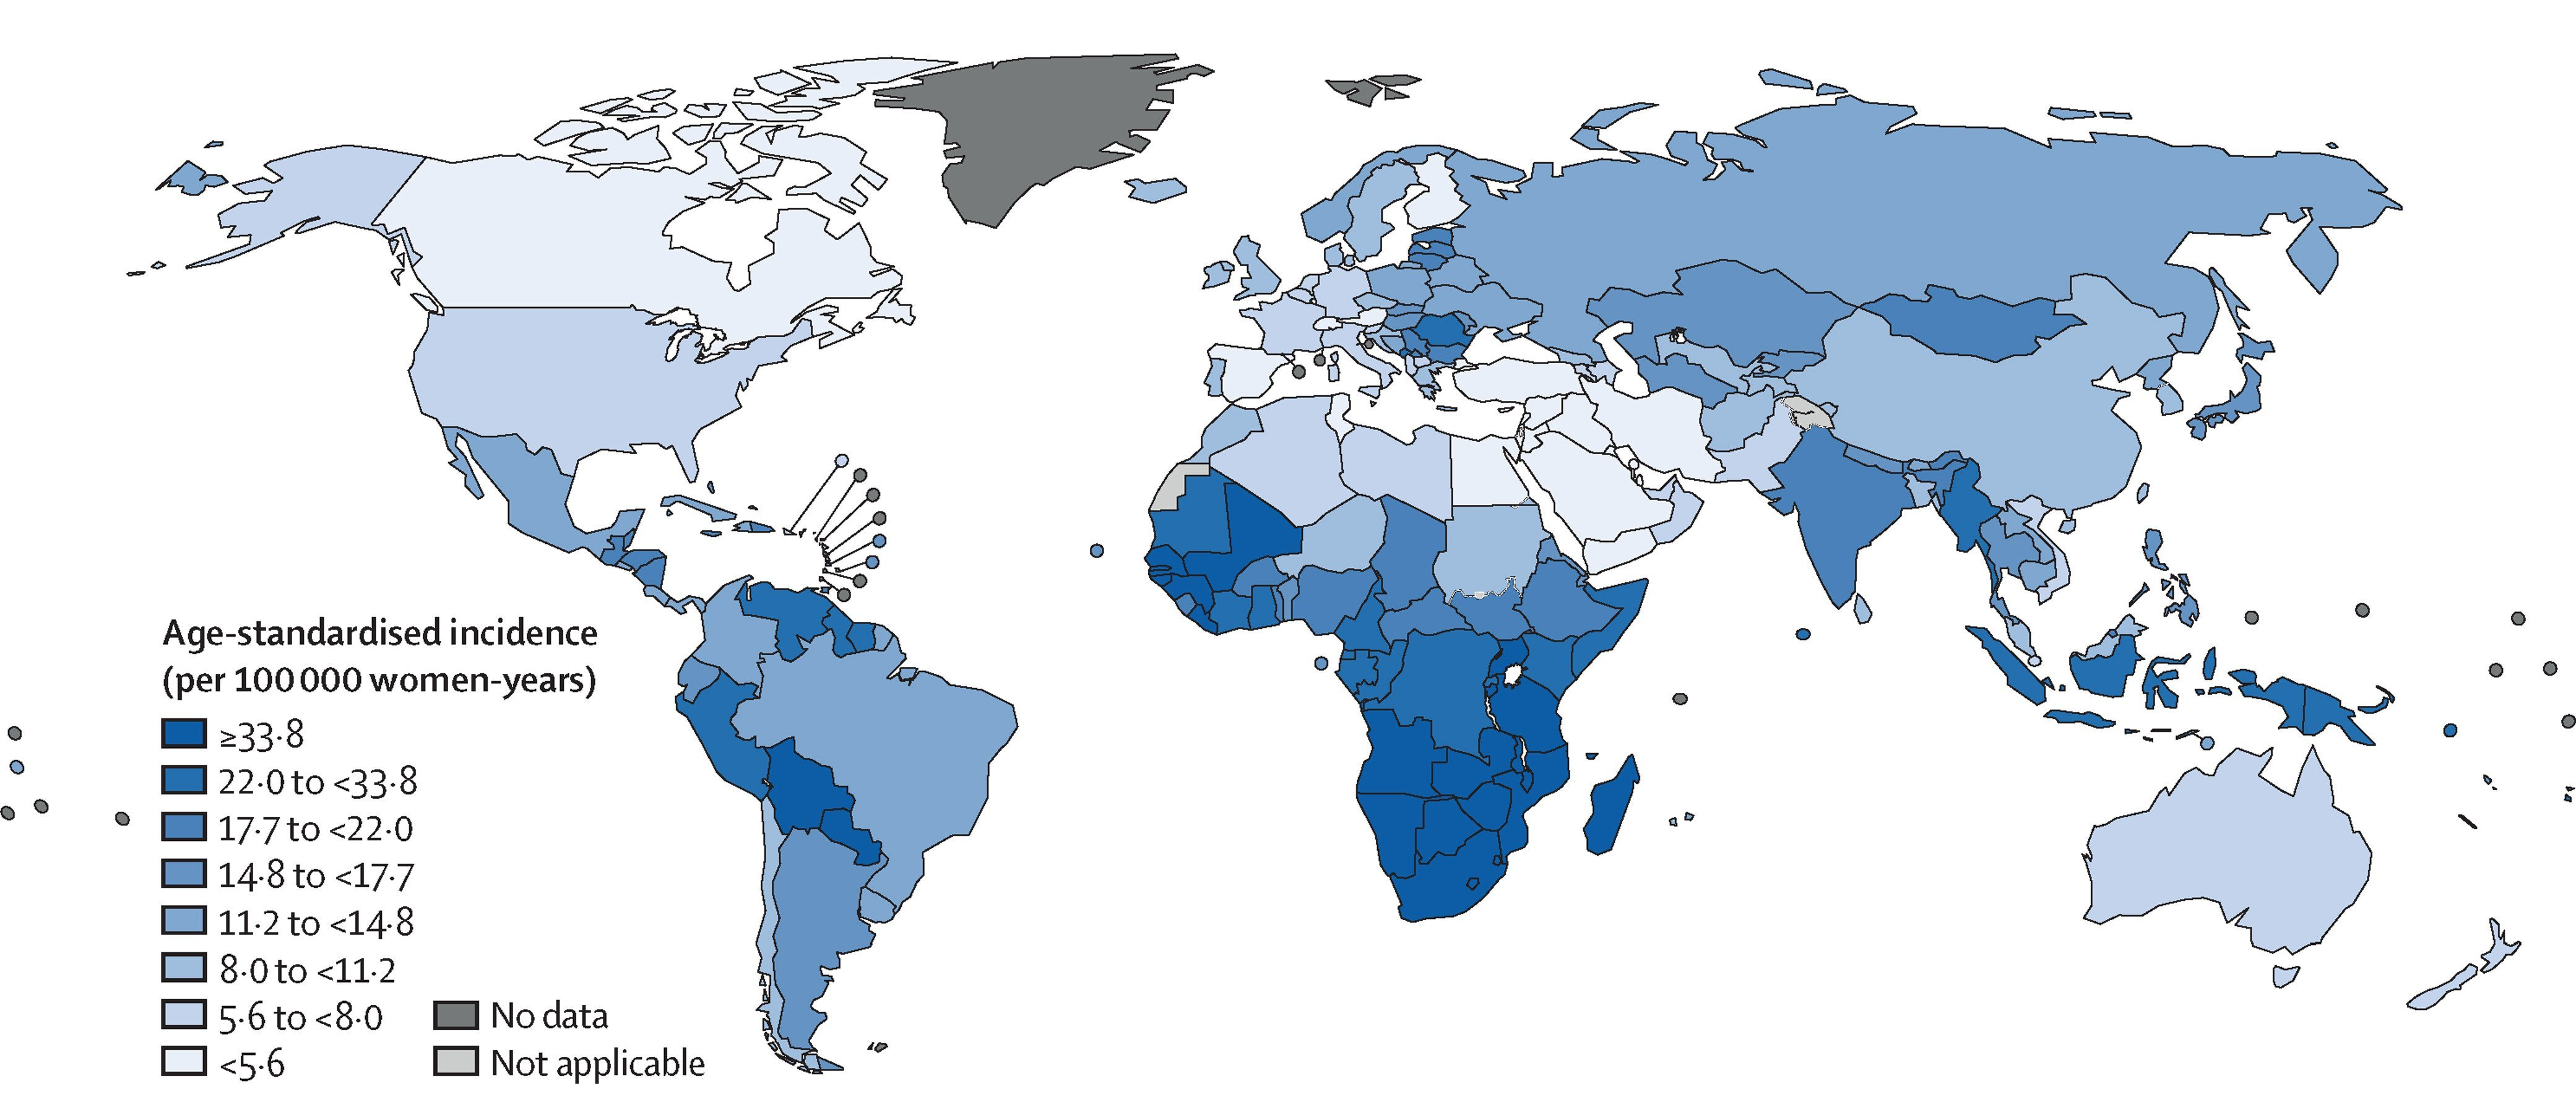
\includegraphics{img/EstadisticaCCervix_A.jpg}

}

}

\subcaption{\label{fig-incidenciaCC1}Incidencia del cáncer de cérvix por
edad}
\end{minipage}%
\newline
\begin{minipage}[t]{\linewidth}

{\centering 

\raisebox{-\height}{

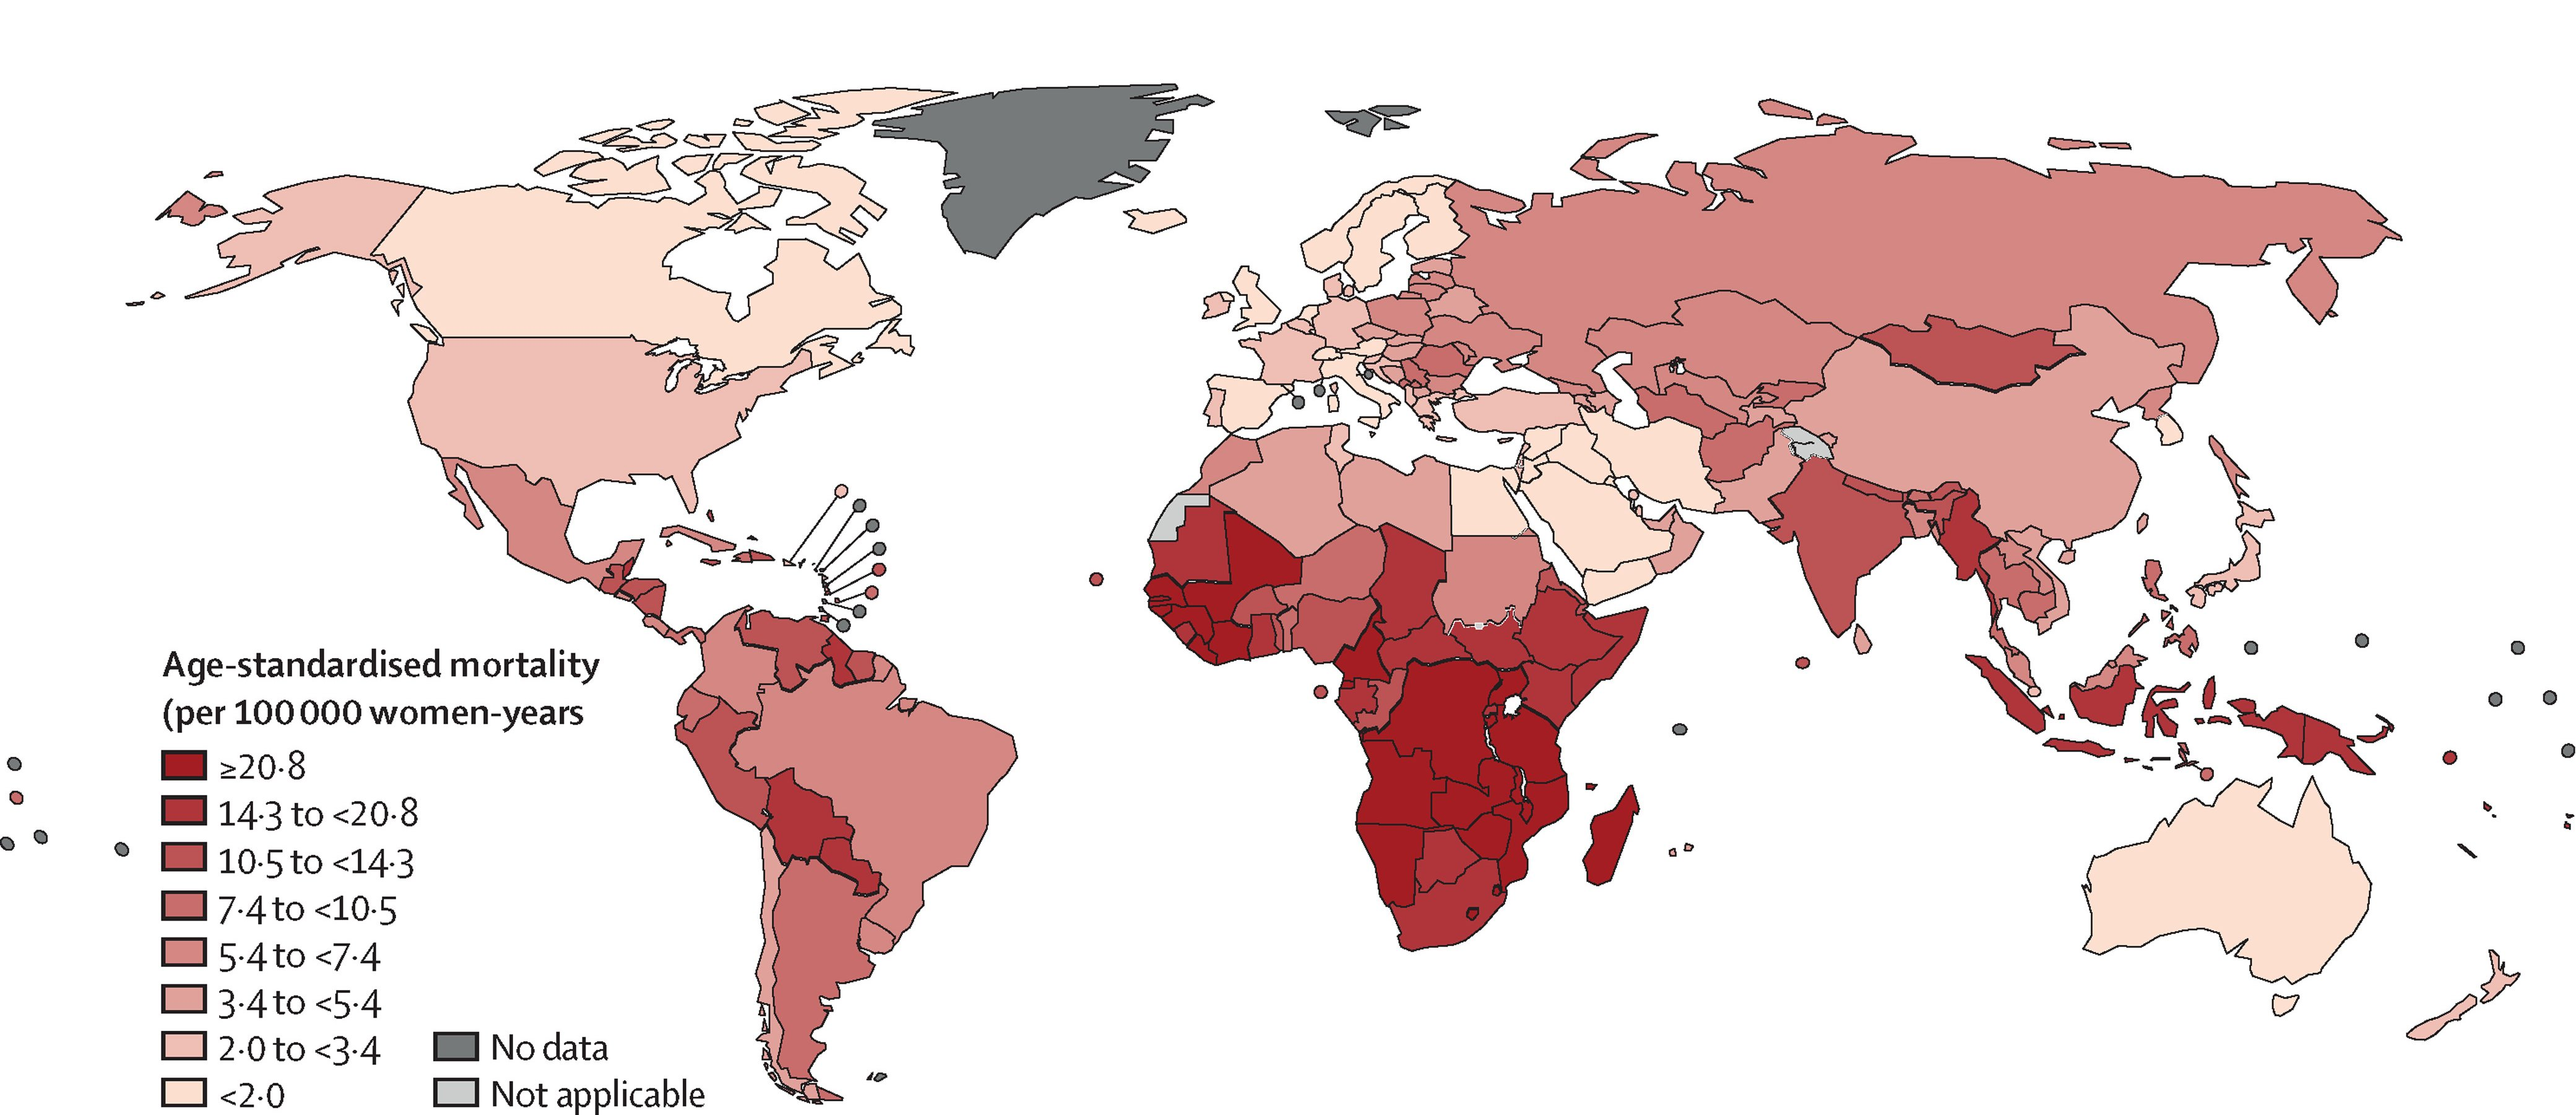
\includegraphics{img/EstadisticaCCervix_B.jpg}

}

}

\subcaption{\label{fig-incidenciaCC2}Mortalidad provocada por el cáncer
de cérvix por edad}
\end{minipage}%

\caption{\label{fig-incidenciaCC}Cáncer de cérvix por paises en 2020.
Datos del (\href{https://gco.iarc.fr/}{Global Cancer Observatory})
(tomado de Singh et
al.\textsuperscript{\protect\hyperlink{ref-singh2023}{9}})}

\end{figure}

\hypertarget{evoluciuxf3n-de-los-sistemas-de-implantaciuxf3n}{%
\subsection{Evolución de los sistemas de
implantación}\label{evoluciuxf3n-de-los-sistemas-de-implantaciuxf3n}}

El origen de los sistemas de implantación (dispositivos utilizados para
administrar y colocar fuentes radiactivas dentro de un tumor o en sus
proximidades), se remonta a comienzos del siglo XX, cuando se
introdujeron por primera vez fuentes radiactivas implantadas manualmente
en los tumores\textsuperscript{\protect\hyperlink{ref-introd2012}{10}}.
En aquel entonces, este enfoque implicaba una exposición no deseada a la
radiación para los médicos y otros profesionales de la salud. Sin
embargo, a mediados del siglo XX, se comenzaron a utilizar técnicas de
carga diferida
(\emph{after-loaders})\textsuperscript{\protect\hyperlink{ref-aronowitz2015}{11}}
(Figura~\ref{fig-afterloader}), en las cuales las agujas huecas o los
aplicadores se colocan en el volumen del tumor insertando posteriormente
las fuentes radiactivas en dichos dispositivos, con lo que la exposición
a la radiación del personal sanitario se redujo de manera importante.

\begin{figure}

\begin{minipage}[t]{\linewidth}

{\centering 

\raisebox{-\height}{

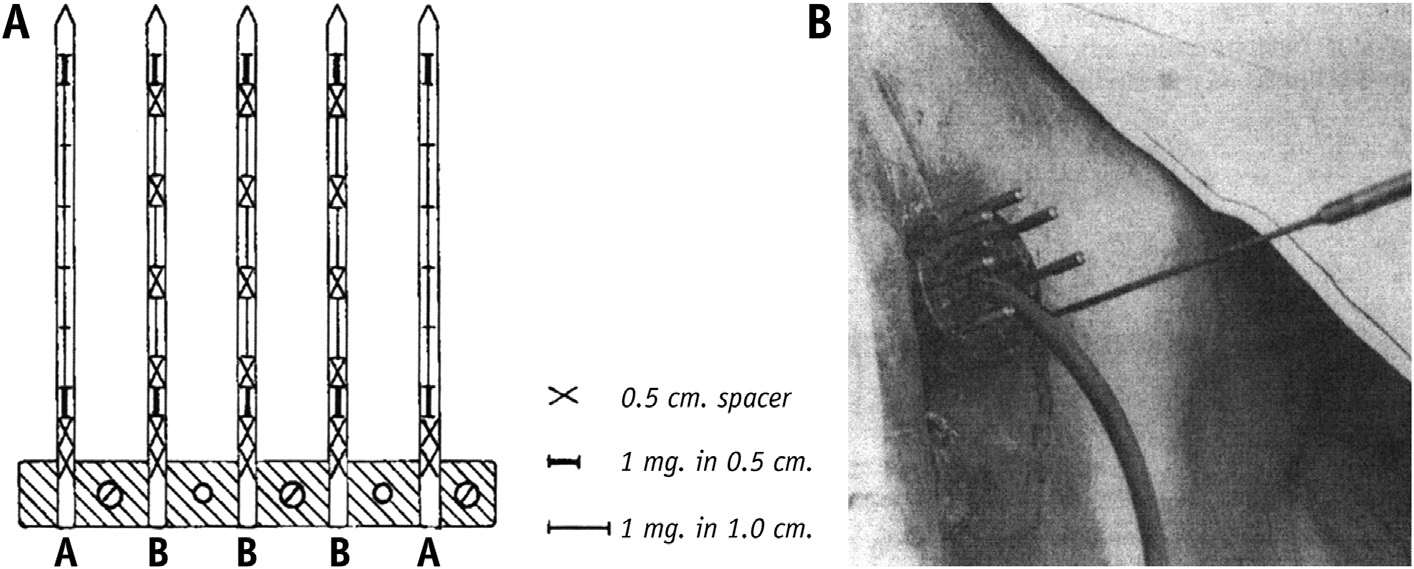
\includegraphics[width=5.20833in,height=\textheight]{img/Afterloader.jpg}

}

}

\subcaption{\label{fig-afterloader}Agujas huecas, para ser cargadas con
semillas de radio de varias longitudes y actividades (y espaciadores
para separar el tren) fueron ideadas en Londres en 1942 para permitir
una carga no homogénea de radio.}
\end{minipage}%
\newline
\begin{minipage}[t]{\linewidth}

{\centering 

\raisebox{-\height}{

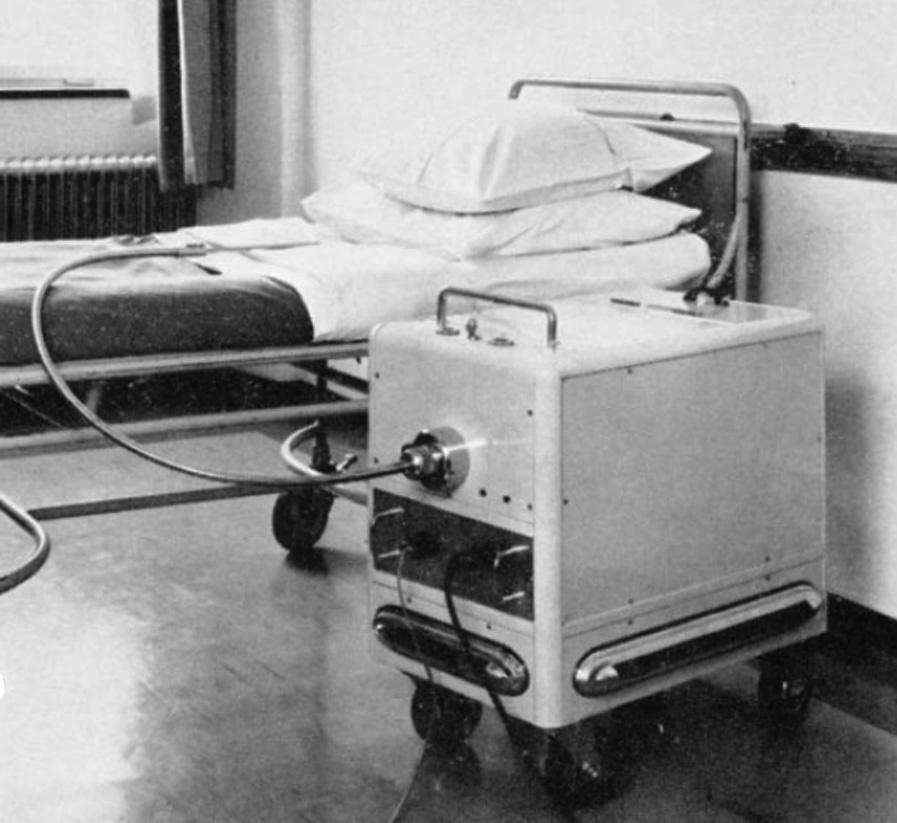
\includegraphics[width=3.64583in,height=\textheight]{img/remoteafterloader.jpg}

}

}

\subcaption{\label{fig-remoteafterloader}El \emph{after-loader} remoto
de un canal y una posición de Walstam (1962).}
\end{minipage}%

\caption{\label{fig-afterloaders}Evolución de los dispositivos de carga
diferida. (Imagen tomada de la publicación de
Aronowitz\textsuperscript{\protect\hyperlink{ref-aronowitz2015}{11}})}

\end{figure}

La llegada de los dispositivos de carga diferida remotos
(Figura~\ref{fig-remoteafterloader}) (RAL) a finales del siglo XX supuso
avances significativos en la práctica de la BT. Dichos dispositivos
remotos permitían la colocación de fuentes radiactivas a distancia en
agujas o aplicadores, reduciendo todavía más las exposiciones a la
radiación. Esta última innovación permitió el uso de fuentes de alta
actividad para aplicaciones de alta tasa de dosis (HDR) y tasa de dosis
pulsada (PDR). La BT de alta tasa de dosis mediante RAL se generalizó en
la segunda mitad de los años ochenta del siglo XX con la aparición de
ordenadores con una mayor capacidad de cálculo y memoria que a su vez
posibilitaron la aparición de los primeros sistemas de planificación
(TPS).

\hypertarget{el-sistema-de-manchester}{%
\subsection{El Sistema de Manchester}\label{el-sistema-de-manchester}}

El sistema de Manchester se desarrolló para la planificación de los
tratamientos de cáncer de cérvix en los años 30 del siglo
XX\textsuperscript{\protect\hyperlink{ref-goodwin1968}{1},\protect\hyperlink{ref-tod1938}{12},\protect\hyperlink{ref-tod1953}{13}}.
Su objetivo era estandarizar la dosimetría y el tratamiento en
diferentes pacientes mediante la definición de puntos de referencia
específicos.

En el Sistema Manchester, los dos puntos de referencia utilizados para
la dosimetría son el Punto A y el Punto B. El punto A corresponde al
triángulo paracervical en el borde medial del ligamento ancho, donde los
vasos uterinos cruzan el uréter. Geométricamente, este punto se definió
trazando una línea que uniera los bordes superiores de los ovoides
vaginales y midiendo 2 cm en dirección superior a lo largo del tándem y
luego 2 cm en dirección perpendicular al tándem.

El punto B, otro punto utilizado en el Sistema de Manchester, representa
los ganglios pélvicos. Originalmente se definió a 5 cm lateralmente
desde la línea media, al mismo nivel que el Punto A. Sin embargo, es
importante señalar que la posición real de los ganglios pélvicos puede
variar de un paciente a otro (Figura~\ref{fig-sistemamanchester}).

El sistema de Manchester consiste en una combinación de tubos
intrauterinos y ovoides, que se insertan en la vagina y el útero de la
paciente\textsuperscript{\protect\hyperlink{ref-yordy2012}{14}}. La
geometría de los aplicadores está diseñada de tal manera que el punto A
recibe la misma dosis, independientemente de la combinación específica
de tubos intrauterinos y ovoides utilizados. Esta característica hizo
que el sistema de Manchester y sus aplicadores fueran más populares que
los disponibles anteriormente y formó la base de los métodos modernos de
aplicación de BT intracavitaria y especificación de dosis.

\begin{figure}

{\centering 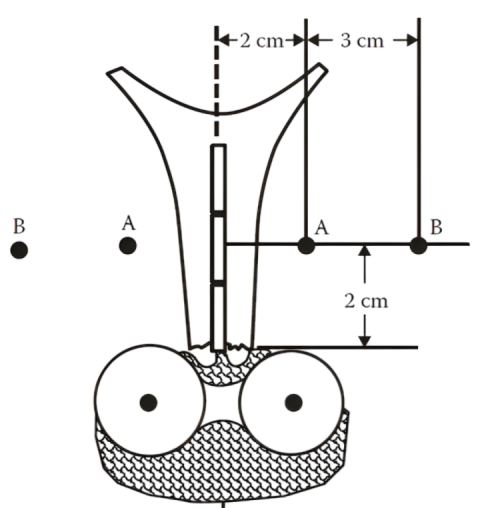
\includegraphics[width=3.125in,height=\textheight]{img/SistemaManchester.png}

}

\caption{\label{fig-sistemamanchester}Diagrama esquemático de los puntos
``A'' y ``B'' en el sistema clásico de Manchester.(Tomado de
ICRU38\textsuperscript{\protect\hyperlink{ref-ICRU38}{15}})}

\end{figure}

A diferencia de los sistemas aplicadores anteriores, los aplicadores
Manchester son fijos y rígidos, lo que reduce la posibilidad de que el
aplicador se deslice y cambie la distribución espacial de la dosis. El
uso de aplicadores precargados y de carga diferida en el sistema de
Manchester también ayudó a superar las limitaciones asociadas con el uso
de aplicadores de radio peligrosos y tiempos de tratamiento prolongados.

El uso histórico del punto A ha sido casi universal, salvo en la escuela
francesa. Hay dos razones principales para este uso generalizado. En
primer lugar, el punto A puede delimitar o no la extensión lateral de
los parametrios, un aspecto esencial de la BT ginecológica. En segundo
lugar, el punto A puede definirse fácilmente incluso en las prácticas
clínicas básicas, lo que permite comparar los resultados clínicos entre
distintos centros. El punto A (y B) ganó popularidad en la primera época
de la BT ginecológica debido a las limitaciones técnicas de entonces,
hasta que aparecieron ordenadores capaces de trabajar con mapas de
dosis.

\hypertarget{sec-introduccionimagen3D}{%
\subsection{La introducción de la imagen
3D}\label{sec-introduccionimagen3D}}

Antes de la aparición de las imágenes en 3D, los sistemas de
planificación y dosimetría del tratamiento de BT se basaban en la
dosimetría de película plana y las técnicas de imágenes en 2D. El uso
del punto A y el punto B como puntos de referencia en BT ginecológica
obtuvo una amplia aceptación debido a su simplicidad y compatibilidad
entre diferentes instalaciones. Sin embargo, las limitaciones de estas
primeras técnicas se hicieron evidentes, ya que proporcionaban
información y precisiones limitadas para predecir los resultados del
tratamiento\textsuperscript{\protect\hyperlink{ref-puxf6tter2001}{16}}.

El uso de imágenes en 3D para la planificación de la BT se introdujo por
primera vez a mediados de la década de 1990 (figura~\ref{fig-plato}), al
generalizarse en los países desarrollados la planificación de
tratamientos de radioterapia de haz externo (EBRT) en 3D sobre imágenes
de tomografía computarizada (CT). Esto permitió realizar planes de
tratamiento basados en volúmenes de manera relativamente rápida y
sencilla. A raíz de esta innovación los avances en EBRT aparecieron los
primeros TPSs de BT que integraban módulos de imágenes 3D. Se observó
que estas secuencias tomográficas proporcionan más información anatómica
y permiten evaluar mejor la definición del tumor, su relación con la
anatomía circundante y los órganos en riesgo, así como la colocación de
los aplicadores o catéteres de BT.

\begin{figure}

{\centering 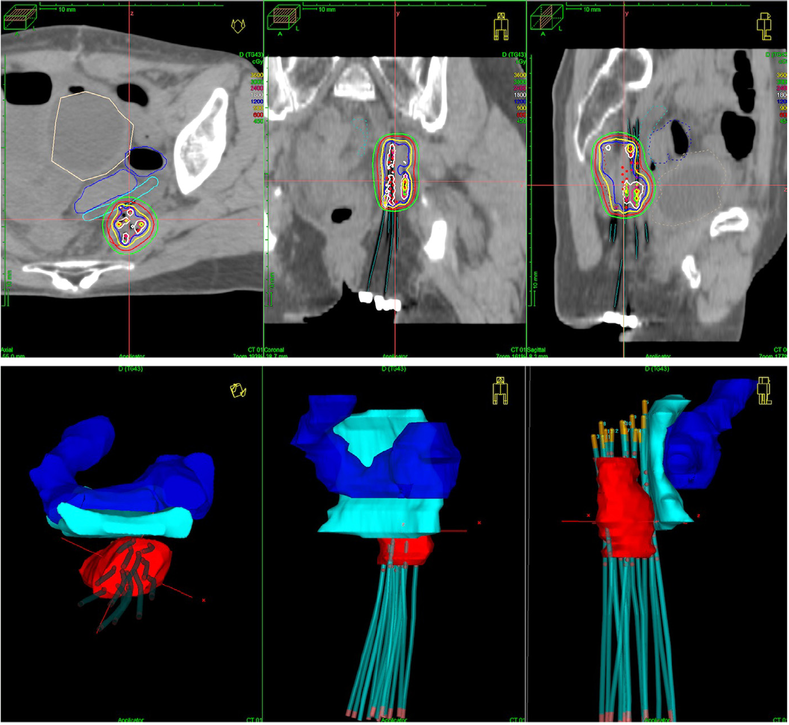
\includegraphics{img/Plato.png}

}

\caption{\label{fig-plato}Planificación de tratamiento de BT calculado
con PLATO (Nucletron, Veenendaal, Países Bajos).(Tomado de Miyata et
al.\textsuperscript{\protect\hyperlink{ref-miyata2023}{17}})}

\end{figure}

Inicialmente, las imágenes de CT proporcionaron mejores cálculos de
dosis dentro de los tumores y los órganos de riesgo en comparación con
la planificación de tratamiento mediante dos placas ortogonales de rayos
X basada en película. Sin embargo, seguía teniendo limitaciones, como la
sobre-estimación de los volúmenes
tumorales\textsuperscript{\protect\hyperlink{ref-onal2009a}{18}}. Dicha
sobre-estimación está relacionada con la limitación del CT en la
definición de los tejidos. Esa es precisamente una de las ventajas que
ofrece la imagen por resonancia magnética nuclear (MRI). Otra de las
ventajas de la mejor definición de los tejidos es la de permitir una
planificación adaptativa, ya que el tumor retrocede con cada fracción
administrada\textsuperscript{\protect\hyperlink{ref-sagae2023}{19}}.

La introducción de la MRI en BT es a comienzos del siglo XXI. En 2005,
el Groupe Europeen de Curietherapie y la Sociedad Europea de
Radioterapia y Oncología (GEC-ESTRO) publicaron unas directrices para la
planificación óptima de los volúmenes objetivo de BT guiada por
MRI\textsuperscript{\protect\hyperlink{ref-haie-meder2005}{20}}. Estas
directrices destacaban la importancia de la MRI para mejorar el control
local y reducir la toxicidad del tejido sano. Estudios y ensayos
posteriores destacaron aún más los beneficios de la BT guiada por MRI.
El ensayo francés STIC de
2012\textsuperscript{\protect\hyperlink{ref-charra-brunaud2012}{21}}
demostró que la BT tridimensional guiada por MRI, era factible y segura
en la práctica rutinaria, con un mejor control local y una menor
toxicidad en comparación con la 2D. El American Brachytherapy Task Group
informó en 2017\textsuperscript{\protect\hyperlink{ref-mayadev2017}{22}}
de que la BT guiada por MRI era más eficaz y segura que las
prescripciones de dosis tradicionales de punto A.

A pesar de estas evidencias, se hizo patente que era necesaria una
adopción más rápida de la planificación basada en MRI en la práctica de
la BT ginecológica. Un estudio publicado en
2010\textsuperscript{\protect\hyperlink{ref-viswanathan2010}{23}},
descubrió que solo el 2\% de los oncólogos radioterápicos utilizaban la
planificación basada en MRI, mientras que la mayoría seguía
prescribiendo en el punto A y registrando la dosis según las
prescripciones del punto de dosis de la
ICRU38\textsuperscript{\protect\hyperlink{ref-ICRU38}{15}}.

\hypertarget{imagen-en-bt-de-cuxe9rvix}{%
\section{Imagen en BT de cérvix}\label{imagen-en-bt-de-cuxe9rvix}}

En la BT de cáncer de cérvix actual se utilizan diferentes tipos de
modalidades de imagen 3D para guiar y planificar el tratamiento. Dichas
modalidades son ultrasonidos, tomografía por emisión de positrones,
tomografía computarizada e imagen por resonancia magnética nuclear.

\hypertarget{ultrasonidos}{%
\subsection{Ultrasonidos}\label{ultrasonidos}}

La ecografía por ultrasonidos es una modalidad de imagen que utiliza
ondas sonoras de alta frecuencia para crear imágenes en tiempo real del
área de interés. La ecografía puede utilizarse en BT cervical para guiar
la inserción de los aplicadores intracavitarios y garantizar una
colocación precisa. La ecografía es beneficiosa en los casos en que el
canal endocervical está estrechado u obliterado, ya que permite una
mejor visualización y evita la perforación durante el procedimiento. Una
ventaja añadida es que es una modalidad de imagen que no utiliza
radiaciones ionizantes, en contraposición a los sistemas de imágenes
descritos en las secciones~\ref{sec-imagePET} .

El médico puede navegar por el cuello uterino utilizando la guía
ecográfica y colocar con precisión los aplicadores, garantizando una
geometría óptima del implante. Esto es crucial, ya que se ha demostrado
que los implantes técnicamente buenos se correlacionan con un mejor
control local y, potencialmente, con mejores resultados de supervivencia
en pacientes con cáncer de cuello uterino. Además, la ecografía puede
ayudar a identificar cualquier anomalía o patología que pueda afectar al
tratamiento de
BT\textsuperscript{\protect\hyperlink{ref-dimopoulos2006}{24}}.

Por diversos motivos, la ecografía aún no se ha adoptado de forma
generalizada para identificar estructuras como el cuello uterino y el
útero en la BT
ginecológica\textsuperscript{\protect\hyperlink{ref-vandyk2021}{25}}. En
primer lugar, aunque los primeros estudios sugirieron que se podían
realizar mediciones mediante ecografía para guiar la planificación del
cáncer de endometrio, estos protocolos no se aplicaron de forma
generalizada y no han sido adoptados en el caso de cáncer de
cérvix\textsuperscript{\protect\hyperlink{ref-van2015}{26}}. En segundo
lugar, el uso de la ecografía en la planificación de la BT se ha visto
obstaculizado por problemas como la mala resolución de la imagen, la
reproducibilidad inadecuada y la visualización sub-óptima de estructuras
críticas\textsuperscript{\protect\hyperlink{ref-St-Amant2017}{27}}. Por
último, existe una curva de aprendizaje asociada a la adquisición,
orientación e interpretación de imágenes, y la ecografía bidimensional
sólo visualiza una vista limitada de la región de interés. Por todo
ello, aunque la ecografía es una modalidad de imagen prometedora,
todavía no se ha extendido como estándar de imagen en BT ginecológica.

\hypertarget{sec-imagePET}{%
\subsection{Tomografía por emisión de positrones
(PET/CT)}\label{sec-imagePET}}

La imagen PET/CT con FDG (18F-fluorodesoxiglucosa) es una herramienta
valiosa para evaluar la extensión del cáncer ginecológico y la respuesta
al tratamiento. La FDG es un radiotrazador que es captado por células
metabólicamente activas, como las cancerosas, lo que permite visualizar
y cuantificar el metabolismo de la glucosa en los tejidos. La
combinación de PET y CT en una única modalidad de imagen proporciona
información tanto funcional como anatómica, permitiendo una localización
y caracterización más precisa de los tumores.

En el contexto de los cánceres ginecológicos, la imagen PET/CT con FDG
se ha utilizado con diversos fines. Se utiliza comúnmente para la
estadificación inicial y la evaluación de la extensión de la enfermedad
en pacientes con neoplasias ginecológicas, incluidos los cánceres de
cuello uterino, endometrio, ovario y vulva. La PET/TC puede ayudar a
identificar tumores primarios, detectar la afectación de ganglios
linfáticos regionales y evaluar la presencia de metástasis a
distancia\textsuperscript{\protect\hyperlink{ref-ora2022}{28}}. Es
especialmente útil para detectar la enfermedad metastásica a distancia,
que es crucial para determinar las estrategias de tratamiento adecuadas
y el pronóstico.

Además, el PET/TC con FDG también puede utilizarse para evaluar la
respuesta al tratamiento en cánceres ginecológicos. Al comparar las
exploraciones PET/CT previas y posteriores al tratamiento, los cambios
en la captación de FDG pueden indicar la eficacia de la terapia y ayudar
a orientar las decisiones
terapéuticas\textsuperscript{\protect\hyperlink{ref-fracasso2022}{29}}.
Una disminución de la captación de FDG después del tratamiento sugiere
una respuesta favorable, mientras que una captación persistente o
aumentada puede indicar enfermedad residual o progresiva. El PET/CT
puede proporcionar información valiosa para monitorizar la respuesta al
tratamiento y ajustar los planes de tratamiento en consecuencia.

Sin embargo, es importante señalar que las imágenes PET/TC con FDG no
son válidas para la BT, que es una modalidad de tratamiento común para
los cánceres ginecológicos. El uso de PET/TC para la planificación de la
BT es limitado debido a varios factores.

En primer lugar, las imágenes PET/CT con FDG tienen limitaciones para
visualizar y delinear con precisión el tumor y los tejidos circundantes
en la pelvis, que es la región de interés para la BT
ginecológica\textsuperscript{\protect\hyperlink{ref-liu2019}{30}}. Los
artefactos de movimiento causados por la respiración o el peristaltismo
gástrico pueden afectar a la calidad de las imágenes de PET/CT, lo que
reduce la precisión en la delineación del tumor. Además, el tiempo de
examen requerido para PET/CT es más largo en comparación con otras
modalidades de imagen, lo que puede no ser factible para la naturaleza
sensible al tiempo de los procedimientos de BT.

En segundo lugar, el uso de PET/CT para la planificación de la BT puede
no proporcionar la suficiente resolución espacial y detalle anatómico
necesarios para la colocación precisa de aplicadores y
agujas\textsuperscript{\protect\hyperlink{ref-liu2019}{30}}. La BT
requiere una localización precisa del tumor y las estructuras
circundantes para garantizar una administración óptima de la radiación y
minimizar el daño a los tejidos sanos. Aunque PET/CT puede proporcionar
información funcional sobre el metabolismo tumoral, es posible que no
proporcione la información anatómica necesaria para la reconstrucción
del aplicador y la planificación del
tratamiento\textsuperscript{\protect\hyperlink{ref-liu2019}{30}}.

\hypertarget{sec-imageCT}{%
\subsection{Tomografía Computarizada}\label{sec-imageCT}}

El CT es una modalidad de imagen ampliamente utilizada en BT
ginecológica para el tratamiento de tumores cervicales. El CT
proporciona información anatómica detallada mediante el uso de rayos X
para crear imágenes transversales del cuerpo. Desempeña un papel crucial
en la planificación del tratamiento, la segmentación del volumen
objetivo y el cálculo de la dosis en los procedimientos de BT.

En BT ginecológica, el CT se utiliza para visualizar la región pélvica y
definir con precisión el tumor y las estructuras circundantes. Las
imágenes de CT ayudan a determinar el tamaño, la ubicación y la
extensión del tumor, así como a identificar cualquier afectación de los
ganglios linfáticos o
metástasis\textsuperscript{\protect\hyperlink{ref-uxf6zsarlak2003}{31}}.
La información obtenida mediante CT es esencial para la planificación
del tratamiento, ya que guía la colocación de aplicadores y
agujas\textsuperscript{\protect\hyperlink{ref-huang2018}{32}}.

El CT puede utilizarse en la BT cervical para proporcionar información
valiosa para la planificación del tratamiento y la optimización de la
dosis a los órganos de riesgo. Su uso está muy extendido y los oncólogos
radioterápicos están familiarizados con su interpretación. La CT permite
delinear los órganos de riesgo (OAR) de forma comparable a la
MRI\textsuperscript{\protect\hyperlink{ref-viswanathan2007}{33}} ,
proporcionando información útil como la posición de la sonda
intrauterina, el grosor del tabique recto-vaginal y la relación entre la
vejiga/rectosigmoide y el aplicador.

Sin embargo, las imágenes de CT tienen ciertas limitaciones cuando se
trata de tratar tumores cervicales en BT. Como se mencionó en la
sección~\ref{sec-introduccionimagen3D}, una limitación es el contraste
relativamente bajo de los tejidos blandos en comparación con otras
modalidades de imagen, como la resonancia magnética. Esto puede
dificultar la delimitación precisa del tumor y las estructuras
circundantes, especialmente en casos de tumores pequeños o cuando el
tumor es isodenso con el tejido cervical
normal\textsuperscript{\protect\hyperlink{ref-uxf6zsarlak2003}{31}}.

Otra limitación de las imágenes de CT en BT es la presencia de
artefactos metálicos causados por los aplicadores metálicos utilizados
en el procedimiento. Estos artefactos pueden oscurecer los tejidos
blandos circundantes y afectar a la precisión de las imágenes de CT,
aunque se han desarrollado técnicas de reducción de artefactos metálicos
para mitigar este problema y mejorar la calidad de las imágenes de CT en
presencia de implantes metálicos.

\hypertarget{resonancia-magnuxe9tica-nuclear}{%
\subsection{Resonancia Magnética
Nuclear}\label{resonancia-magnuxe9tica-nuclear}}

La MRI es una sofisticada técnica médica de diagnóstico por imagen. A
diferencia de los rayos X, que emplean radiaciones ionizantes, la MRI
utiliza potentes campos magnéticos y ondas de radiofrecuencia para
generar imágenes sin exponer a los pacientes a radiaciones ionizantes.

El principio de la resonancia magnética nuclear se basa en el
comportamiento de los núcleos atómicos cuando se someten a un campo
magnético intenso y a determinados pulsos de radiofrecuencia (RF). En
concreto, los núcleos (normalmente núcleos de hidrógeno o protones) se
alinean con el campo magnético externo como si fuesen pequeños imanes.

Las máquinas de resonancia magnética nuclear (MR) disponen de potentes
imanes que crean un campo magnético sólido y uniforme. También hay
bobinas que inducen campos magnéticos adicionales con un gradiente de
campo que varían a través del espacio. Estos campos son los responsables
de la codificación espacial en las imágenes resultantes. El flujo
general de trabajo de una máquina de MRI sería:

\begin{enumerate}
\def\labelenumi{\arabic{enumi}.}
\item
  \textbf{Pulso de RF y excitación:} Para generar una imagen de RM, el
  paciente se coloca dentro de la máquina de RM. Se envía un pulso
  inicial de RF, que altera temporalmente la alineación de los momentos
  magnéticos de los protones. Este proceso se conoce como excitación.
\item
  \textbf{Relajación y emisión de la señal:} Los protones vuelven a su
  estado alineado después de que se apague el pulso de RF. Este proceso
  implica la relajación T1 (relajación longitudinal) y la relajación T2
  (relajación transversal). A medida que los protones se relajan, emiten
  señales de radiofrecuencia, que la máquina de MR puede detectar.
\item
  \textbf{Detección y procesamiento de señales:} Las señales emitidas
  son detectadas por bobinas de radiofrecuencia situadas alrededor del
  cuerpo del paciente. Estas bobinas captan señales de radiofrecuencia
  débiles, cuya intensidad varía en función de las propiedades del
  tejido local. A continuación, el sistema informático de la máquina de
  MR procesa las señales.
\item
  \textbf{Codificación espacial:} Las bobinas de gradiente desempeñan un
  papel crucial en la codificación espacial de las señales. La máquina
  de MR puede determinar el origen de la señal dentro del cuerpo
  aplicando campos de gradiente controlados y variables. Esta
  información se utiliza para crear un mapa espacial de las señales
  emitidas.
\item
  \textbf{Reconstrucción de imágenes:} Las señales recogidas se procesan
  matemáticamente para crear una imagen 2D o 3D. Los distintos tipos de
  tejidos y estructuras tienen tiempos de relajación diferentes, lo que
  contribuye al contraste de las imágenes finales.
\end{enumerate}

Para obtener una imagen óptima de MRI para el tratamiento, se deben
cumplir unos criterios específicos. Los requisitos técnicos incluyen MR
de campo principal igual o superior a 1.5 T, bobinas de superficie
pélvica y software para la adquisición, transferencia y contorneado de
imágenes\textsuperscript{\protect\hyperlink{ref-richart2018}{34},\protect\hyperlink{ref-dimopoulos2012}{35}}.
La preparación del paciente implica la inmovilización, el llenado de la
vejiga y la evacuación
intestina\textsuperscript{\protect\hyperlink{ref-dimopoulos2012}{35}}.
Las secuencias de MRI más útiles son la T2 para visualizar la anatomía y
la colocación del
aplicador\textsuperscript{\protect\hyperlink{ref-dimopoulos2012}{35},\protect\hyperlink{ref-petric2014}{36}}.
Secuencias adicionales como la T1 con contraste o la isotrópica 3D
pueden proporcionar información
complementaria\textsuperscript{\protect\hyperlink{ref-richart2018}{34}}.

En cuanto a la magnitud de campo principal de una MR, existen varias
ventajas de utilizar un campo de 3 T en lugar de un campo de 1.5 T para
BT de cérvix. Una de las principales es la mayor relación señal-ruido
(SNR) que proporciona una MR de 3 T además de una mejora en la
resolución espacial. Estos factores resultan en una mejor calidad de
imagen, lo que incrementa la precisión en la segmentación de objetos y
por tanto en la planificación del tratamiento. También permite la
visualización de estructuras más pequeñas mejorando la detección de
anomalías
sutiles\textsuperscript{\protect\hyperlink{ref-kataoka2007}{37}}.

Además, una MR de 3 T puede reducir el tiempo de exploración necesario
para la adquisición de imágenes. La mayor SNR y resolución espacial que
proporciona una MR de 3 T permite una adquisición de imágenes más rápida
sin comprometer la calidad de la imagen. Esto puede mejorar la comodidad
del paciente y la eficiencia del flujo de trabajo en el entorno clínico.

No obstante, aunque utilizar una MR de 3 T en lugar de una de 1.5 T
ofrece ventajas, hay que tener en cuenta ciertos inconvenientes. Uno de
los principales inconvenientes es la mayor susceptibilidad a los
artefactos y las distorsiones a intensidades de campo más elevadas. La
presencia de implantes o aplicadores metálicos pueden causar artefactos
de susceptibilidad, afectando a la precisión de las secuencias de
MRI\textsuperscript{\protect\hyperlink{ref-kumar2020}{38}}. Además, el
aumento de la intensidad del campo magnético puede provocar una mayor
deposición de potencia de RF en el paciente, lo que puede afectar a la
seguridad de este.

Otro inconveniente es el mayor coste de utilizar una MR de 3 T en
comparación con una de 1.5 T. Los costes de adquisición y mantenimiento
de un sistema de RM MR de 3 T son más elevados, lo que puede limitar su
disponibilidad y accesibilidad en determinados entornos sanitarios.

Respecto a equipos de MR con campos principales mayores de 7 T como el
MAGNETOM TERRA de Siemens Healthineers o del SIGNA 7.0T de GE
Healthcare, no hay todavía estudios de su uso en BT.

\hypertarget{registro-de-imuxe1genes}{%
\subsection{Registro de imágenes}\label{registro-de-imuxe1genes}}

El registro de imágenes consiste en alinear y superponer imágenes
adquiridas por separado para crear una imagen fusionada que combine la
información de ambas. Esta fusión permite combinar la información
suministrada por cada uno de los grupos de imágenes iniciales. El
registro más habitual que se realiza en la BT de cérvix es entre CT y
MRI.

\begin{figure}

{\centering 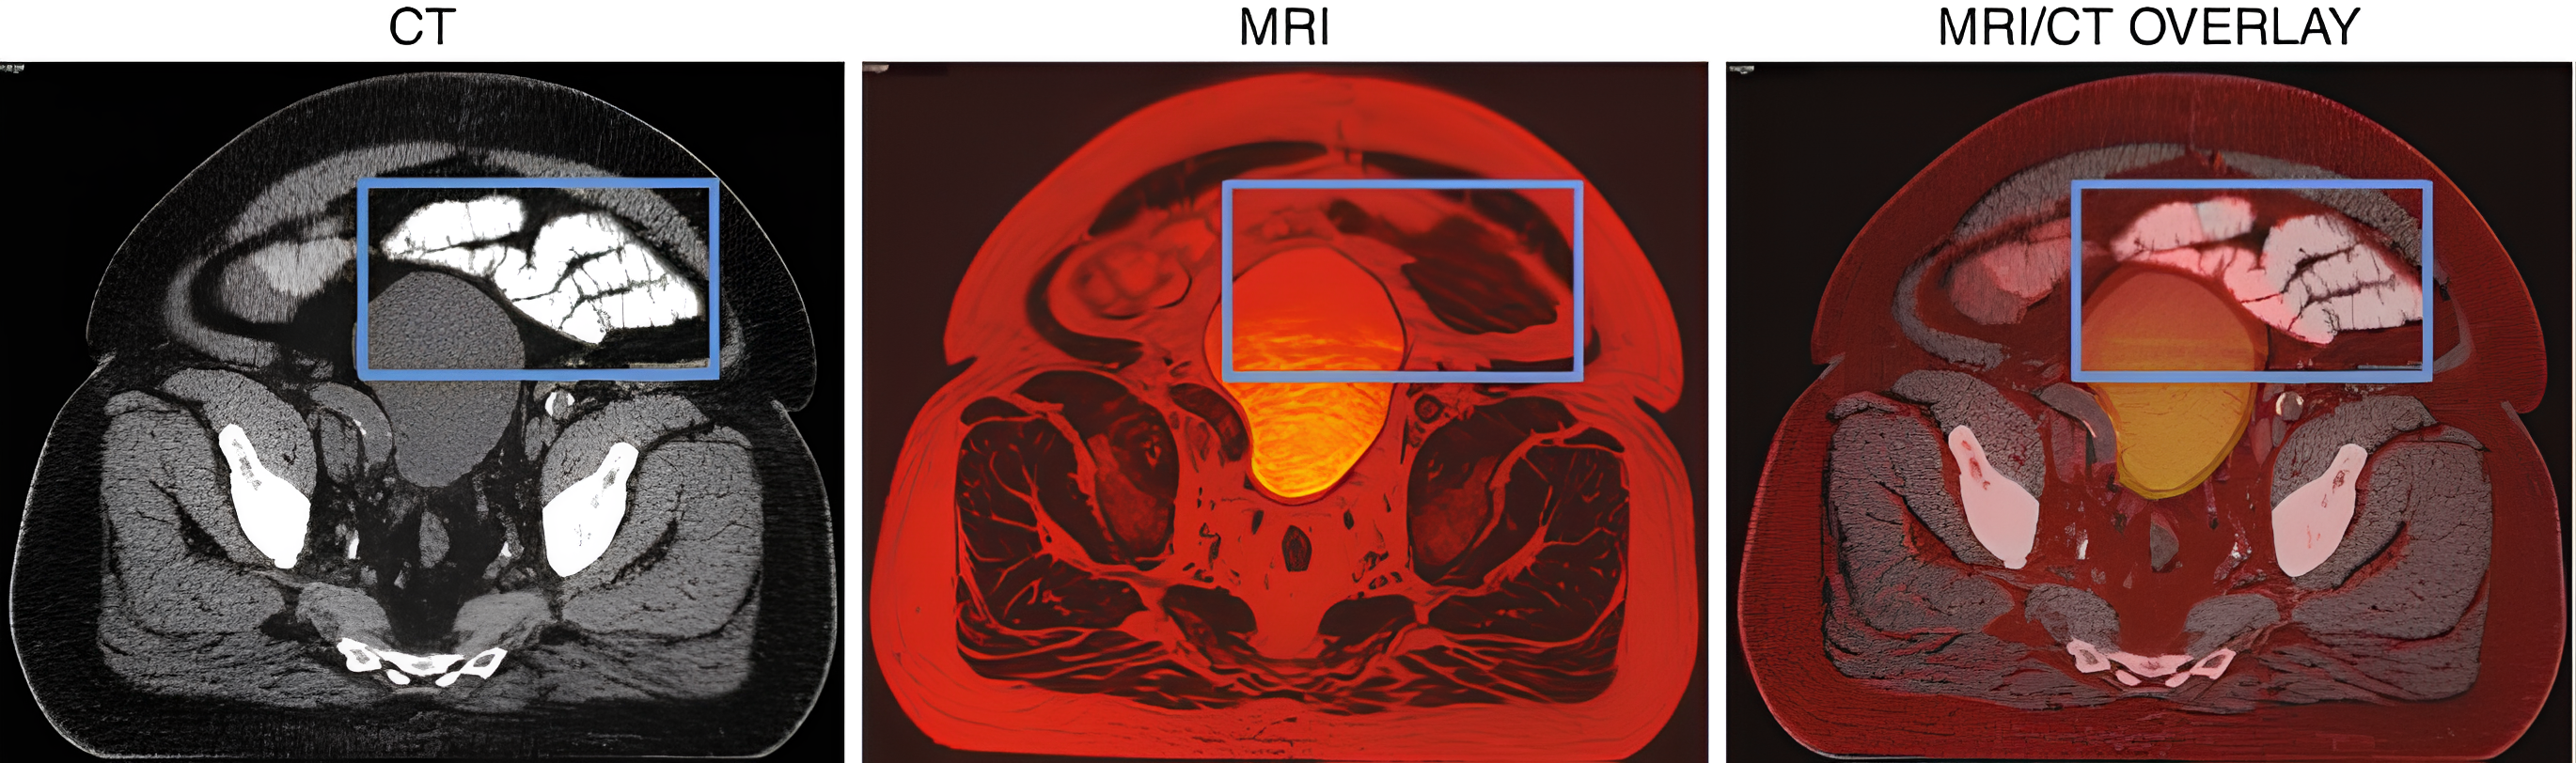
\includegraphics{img/MRI_CT_register.png}

}

\caption{Registro de MRI y CT de la región pélvica(Tomado de
Speight\textsuperscript{\protect\hyperlink{ref-speight2019}{39}})}

\end{figure}

Existen dos tipos principales de registro de imágenes: registro rígido y
registro deformable. El registro rígido consiste en alinear las imágenes
aplicando transformaciones de traslación, rotación y escalado. Asume que
las estructuras anatómicas de las imágenes mantienen su forma y tamaño.
El registro rígido se basa en la suposición de que las posiciones
relativas de las estructuras permanecen constantes entre las imágenes de
CT y MR.

El registro deformable, por otro lado, permite transformaciones más
complejas al tener en cuenta las deformaciones locales y los cambios de
forma entre las imágenes. Tiene en cuenta la naturaleza no lineal y no
rígida de las estructuras anatómicas. Los algoritmos de registro
deformable utilizan modelos matemáticos para estimar el campo de
deformación que mejor alinea las imágenes.

Por otro lado el registro de imágenes influye de manera importante sobre
las incertidumbres en los parámetros de los histogramas dosis-volumen
(DVH)\textsuperscript{\protect\hyperlink{ref-richart2018}{34}}. Tanderup
et al.\textsuperscript{\protect\hyperlink{ref-tanderup2008}{40}}
encontraron que las incertidumbres en la reconstrucción del aplicador,
como las traslaciones y rotaciones, pueden influir más en los parámetros
DVH del recto y la vejiga, especialmente en la dirección
anteroposterior. Demostraron que las desviaciones en estos parámetros
pueden ser de hasta un 5-6\% por mm de desplazamiento del aplicador.
Schindel et
al.\textsuperscript{\protect\hyperlink{ref-schindel2013}{41}} analizaron
el efecto de los desplazamientos del tándem y los ovoides en su
conjunto, así como las incertidumbres de reconstrucción inducidas al
desplazar el tándem y los ovoides de forma independiente en la dirección
cráneocaudal. Descubrieron que el D2cc del recto es el parámetro más
sensible a los desplazamientos, cambiando aproximadamente un 10\% por
cambio de ±1.5 mm. Para evitar cambios dosimétricos superiores al 10\%,
las incertidumbres de la reconstrucción deben mantenerse dentro de los 3
mm.

\begin{tcolorbox}[enhanced jigsaw, leftrule=.75mm, bottomtitle=1mm, colframe=quarto-callout-note-color-frame, toptitle=1mm, breakable, colbacktitle=quarto-callout-note-color!10!white, colback=white, titlerule=0mm, toprule=.15mm, title=\textcolor{quarto-callout-note-color}{\faInfo}\hspace{0.5em}{Nota}, coltitle=black, arc=.35mm, rightrule=.15mm, bottomrule=.15mm, left=2mm, opacityback=0, opacitybacktitle=0.6]

Según ICRU89\textsuperscript{\protect\hyperlink{ref-ICRU89}{42}}, los
parámetros en forma de \(D_V\) se definen como la dosis recibida por al
menos un volumen V, donde V se da como porcentaje de una región definida
o en unidades de cc. Los parámetros \(V_D\) son el volumen que recibe
dosis superiores o iguales a la dosis absorbida D especificada como la
dosis absorbida.

\end{tcolorbox}

Hay que tener en cuenta que cuando se utilizan tomografías
computarizadas como modalidad de imagen de respaldo, el registro con MRI
debe realizarse con cuidado. Oinam et
al.\textsuperscript{\protect\hyperlink{ref-oinam2014}{43}} informan de
un método de reconstrucción que utiliza un registro rígido entre CT y
MRI, y evalúan las incertidumbres del registro. Descubrieron que el
impacto de las incertidumbres en el registro sobre los parámetros DVH de
la vejiga, el recto y el sigmoide es muy sensible a los desplazamientos
anteroposteriores. El D2cc del recto también se ve afectado en gran
medida por las incertidumbres del registro cráneocaudal. Sin embargo,
concluyen que el registro rígido del aplicador entre los estudios de
imágenes de TC y RM es factible y está ampliamente informado en la
literatura.

Otro reto es la presencia de artefactos metálicos en las imágenes de CT,
especialmente cuando se utilizan aplicadores de BT metálicos. Estos
artefactos pueden distorsionar las imágenes de CT y dificultar el
proceso de registro. Se pueden emplear técnicas especializadas, como
algoritmos de reducción de artefactos metálicos, para mitigar estos
artefactos y mejorar la precisión del
registro\textsuperscript{\protect\hyperlink{ref-katsura2018}{44}}.

Además, el registro manual de imágenes introduce la posibilidad de error
humano y subjetividad. La exactitud del registro depende de la pericia y
precisión del operador a la hora de identificar los puntos o regiones
correspondientes en las imágenes de CT y MR. Los métodos de registro
automatizados o semiautomatizados, como los basados en el aprendizaje
profundo, han demostrado ser prometedores para mejorar la precisión y la
eficiencia del proceso de
registro\textsuperscript{\protect\hyperlink{ref-shi2022}{45}}.

\hypertarget{esquema-de-tratamiento-actual-del-cuxe1ncer-de-cuello-de-uxfatero}{%
\section{Esquema de tratamiento actual del cáncer de cuello de
útero}\label{esquema-de-tratamiento-actual-del-cuxe1ncer-de-cuello-de-uxfatero}}

\hypertarget{sec-braqnoopcional}{%
\subsection{Importancia del tratamiento con
BT.}\label{sec-braqnoopcional}}

Numerosos estudios destacan el papel fundamental de la BT intracavitaria
en la consecución de resultados curativos para el cáncer de cuello de
útero localmente avanzado, a menudo administrada tras radioterapia de
haz externo (EBRT) con quimioterapia concurrente. Uno de estos estudios,
realizado en el Centro Oncológico M. D. Anderson de la Universidad de
Texas\textsuperscript{\protect\hyperlink{ref-logsdon1999}{46}}, exploró
la influencia de los cambios en la política de tratamiento sobre los
resultados de la radioterapia para la enfermedad en estadio IIIB
FIGO\footnote{El carcinoma de células escamosas de cuello uterino en
  estadio IIIB de FIGO representa un estadio avanzado de cáncer de
  cuello uterino en el que el tumor se ha extendido a la pared pélvica,
  causando invasión parametrial y/o hidronefrosis o riñón no funcional.}.
Demostró que las estrategias de tratamiento que ponían mayor énfasis en
la radioterapia intracavitaria arrojaban los mejores resultados. Además,
las directrices de la \emph{American Brachytherapy Society}
(ABS)\textsuperscript{\protect\hyperlink{ref-viswanathan2012a}{5},\protect\hyperlink{ref-viswanathan2012}{47}}
así como la The Groupe Européen de Curiethérapie (GEC) and the European
SocieTy for Radiotherapy \& Oncology
(ESTRO)\textsuperscript{\protect\hyperlink{ref-dimopoulos2012}{35}}
recomiendan que la BT debe incluirse como componente de la radioterapia
definitiva para el carcinoma cervical, ya que disminuye las recidivas y
las complicaciones cuando se utiliza junto con la EBRT.

\begin{tcolorbox}[enhanced jigsaw, leftrule=.75mm, bottomtitle=1mm, colframe=quarto-callout-note-color-frame, toptitle=1mm, breakable, colbacktitle=quarto-callout-note-color!10!white, colback=white, titlerule=0mm, toprule=.15mm, title=\textcolor{quarto-callout-note-color}{\faInfo}\hspace{0.5em}{Nota}, coltitle=black, arc=.35mm, rightrule=.15mm, bottomrule=.15mm, left=2mm, opacityback=0, opacitybacktitle=0.6]

La clasificación de los estadíos del cáncer de cérvix más utilizada es
la de la FIGO (Fédération Internationale de Gynécologie et
d'Obstétrique), pudiendose encontrar dicha clasificación en
ICRU89\textsuperscript{\protect\hyperlink{ref-ICRU89}{42}}

\end{tcolorbox}

Además, otros estudios han demostrado la eficacia de la quimioterapia
concurrente con la radioterapia en el tratamiento del cáncer de cuello
uterino localmente avanzado. Por ejemplo, un estudio en el que se
comparó la radiación pélvica con quimioterapia concurrente con la
radiación pélvica y para-aórtica para el cáncer de cuello uterino de
alto riesgo demostró mejores resultados con la adición de quimioterapia
concurrente\textsuperscript{\protect\hyperlink{ref-pelvicr1999}{48}}. En
otro estudio se observó que la radioterapia y la quimioterapia
simultáneas con cisplatino mejoraban los resultados del cáncer de cuello
uterino localmente
avanzado\textsuperscript{\protect\hyperlink{ref-concurre1999}{49}}.

Por lo tanto, teniendo en cuenta los resultados de estos estudios, se
puede justificar que un enfoque de tratamiento equilibrado consistente
en radioterapia de haz externo (RHE) con quimioterapia concurrente
seguida de BT intracavitaria desempeña un papel fundamental en la
consecución de resultados curativos para el cáncer de cuello uterino
localmente avanzado.

En efecto, el panorama del tratamiento del cáncer de cuello uterino ha
evolucionado con la introducción de nuevas técnicas de EBRT, como la
radioterapia de intensidad modulada (IMRT), la terapia de arco
volumétrico modulado (VMAT), la radioterapia corporal estereotáctica
(SBRT) y la terapia con protones. Estas técnicas ofrecen una mayor
precisión y conformación en la administración de la radiación a la zona
diana, al tiempo que minimizan el daño a los tejidos sanos circundantes.
Como consecuencia, en algunas zonas de Estados Unidos se ha tendido a
utilizar exclusivamente tratamientos de EBRT, excluyendo el uso de
BT\textsuperscript{\protect\hyperlink{ref-gill2014}{50}}.

Sin embargo, los estudios han indicado que la incorporación de la BT en
el plan de tratamiento del cáncer de cuello uterino es crucial para
lograr resultados óptimos. Las investigaciones han demostrado que la BT
puede administrar dosis significativamente más altas de radiación al
tumor primario, minimizando al mismo tiempo la dosis a los órganos
críticos de riesgo, como el intestino y la
vejiga\textsuperscript{\protect\hyperlink{ref-tanderup2014a}{51}}.
Además, los pacientes tratados con radioterapia externa y braquiterapia
tenían una tasa significativamente mejor de supervivencia general en
comparación con aquellos tratados únicamente con radioterapia
externa\textsuperscript{\protect\hyperlink{ref-han2013}{52}}.

Por lo tanto, a pesar de los avances en las técnicas de EBRT, excluir la
BT del tratamiento del cáncer de cuello uterino puede provocar una
disminución de la supervivencia tanto específica como
global\textsuperscript{\protect\hyperlink{ref-tanderup2014a}{51}}. Es
importante reconocer las pruebas que respaldan los beneficios de la BT y
garantizar su incorporación en el plan de tratamiento de todos los casos
factibles de cáncer de cuello uterino.

Varios organismos de expertos, como la Sociedad de Oncología
Ginecológica, la ABS y la \emph{National Comprehensive Cancer Network},
han recomendado colectivamente no sustituir la BT por terapias
conformadas de haz externo en la radioterapia primaria con intención
curativa para el cáncer de cuello uterino. Estas recomendaciones se
basan en una amplia investigación y en el análisis de los resultados del
tratamiento, que han demostrado sistemáticamente el papel esencial de la
BT en el tratamiento del cáncer de cuello
uterino\textsuperscript{\protect\hyperlink{ref-holschneider2019}{53},\protect\hyperlink{ref-nationalcomprehensivecancernetworkCervicalCancerVersion}{54}}.
Los estudios han demostrado que la BT mejora significativamente las
tasas de supervivencia y la supervivencia específica de la enfermedad en
pacientes con cáncer de cuello de útero en comparación con la
radioterapia de haz externo sola o con modalidades alternativas. Por lo
tanto, estas organizaciones de expertos abogan por el uso continuado de
la BT como componente integral de la radioterapia primaria con intención
curativa para el cáncer de cuello de útero con el fin de garantizar los
mejores resultados posibles para las pacientes.

\hypertarget{bt-intracavitaria-e-intersticial}{%
\subsection{BT intracavitaria e
intersticial}\label{bt-intracavitaria-e-intersticial}}

Existen dos modalidades principales de BT para el cáncer de cuello de
útero: la BT intracavitaria y una combinación de BT intracavitaria e
intersticial.

La BT intracavitaria implica el uso de un aplicador intracavitario, como
un tándem y ovoides o cilindros vaginales, para colocar la fuente de
radiación dentro de la cavidad corporal, concretamente el útero o la
vagina. Esta técnica se utiliza habitualmente y se ha demostrado que
proporciona un control local eficaz para los cánceres de cuello uterino
en estadio
temprano\textsuperscript{\protect\hyperlink{ref-murofushi2020}{55}}. La
BT intracavitaria administra radiación al tumor y a los tejidos
circundantes dentro de la cavidad corporal, dirigiéndose al tumor
primario y a las zonas adyacentes con riesgo de diseminación
tumoral\textsuperscript{\protect\hyperlink{ref-aggarwal2018}{56}}. Es
una técnica relativamente sencilla y menos invasiva en comparación con
la BT intersticial.

Por otro lado, una combinación de BT intracavitaria e intersticial
implica el uso tanto de aplicadores intracavitarios como de agujas
intersticiales . En este enfoque, el aplicador intracavitario se utiliza
para administrar la radiación al tumor dentro de la cavidad corporal,
mientras que las agujas intersticiales se insertan en el tejido que
rodea el cuello uterino para administrar la radiación directamente al
tumor y a los tejidos circundantes. Esta técnica combinada permite una
focalización más precisa del tumor y proporciona una mejor cobertura de
los tumores más grandes o
complejos\textsuperscript{\protect\hyperlink{ref-fabian2019}{57}}. A
menudo se utiliza en casos en los que la BT intracavitaria por sí sola
puede no proporcionar dosis de radiación adecuadas a todo el
tumor\textsuperscript{\protect\hyperlink{ref-murofushi2020}{55}}.

Las ventajas de la BT intracavitaria incluyen su simplicidad, facilidad
de uso y menor invasividad en comparación con una combinación de BT
intracavitaria e intersticial. La BT intracavitaria se puede realizar
utilizando aplicadores estándar, como tándem y ovoides o cilindros
vaginales, que están fácilmente disponibles y se utilizan habitualmente
en la práctica
clínica\textsuperscript{\protect\hyperlink{ref-aggarwal2018}{56}}.
Requiere la inserción de menos agujas o catéteres en el tejido, lo que
reduce la complejidad del procedimiento y el potencial de
complicaciones. La BT intracavitaria también permite preservar
relativamente los tejidos circundantes, como la vejiga y el recto,
debido a la proximidad de la fuente de radiación al tumor.

Sin embargo, la BT intracavitaria puede tener algunas limitaciones en
comparación con una combinación de BT intracavitaria e intersticial. Una
posible desventaja es la capacidad limitada de administrar radiación a
todo el volumen tumoral, especialmente en casos con tumores voluminosos
o extensos\textsuperscript{\protect\hyperlink{ref-ohkubo2013}{58}}. La
BT intracavitaria por sí sola puede no proporcionar dosis de radiación
adecuadas a todo el tumor, lo que da lugar a un control tumoral
subóptimo\textsuperscript{\protect\hyperlink{ref-murofushi2020}{55}}. En
estos casos, una combinación de BT intracavitaria e intersticial permite
una mejor cobertura del tumor y una mejor distribución de la
dosis\textsuperscript{\protect\hyperlink{ref-tan2015}{59}}. Además, la
BT intersticial se puede utilizar para tratar zonas específicas del
tumor o zonas con menor respuesta a la radiación, lo que proporciona un
enfoque de tratamiento más adaptado y
personalizado\textsuperscript{\protect\hyperlink{ref-fabian2019}{57}}.

\hypertarget{recomendaciones-de-la-abs-y-la-gec-estro}{%
\subsection{Recomendaciones de la ABS y la
GEC-ESTRO}\label{recomendaciones-de-la-abs-y-la-gec-estro}}

Entre los años 2005 y 2012 se publicaron 4 artículos por la
GEC-ESTRO\textsuperscript{\protect\hyperlink{ref-haie-meder2005}{20},\protect\hyperlink{ref-dimopoulos2012}{35},\protect\hyperlink{ref-potter2006}{60},\protect\hyperlink{ref-hellebust2010}{61}}
con el objetivo de brindar recomendaciones para la planificación del
tratamiento en BT de cérvix utilizando imágenes 3D. Estos artículos
abordan conceptos y términos, parámetros de volumen de dosis y aspectos
de anatomía, física de la radiación y radiobiología. Era su intención
también la de establecer un lenguaje común para mejorar la precisión y
la consistencia en la planificación del tratamiento, permitiendo que
diferentes centros y expertos se comunicasen de manera efectiva y se
comprendieran las especificaciones clínicas y técnicas necesarias para
la BT cervical. Al utilizar un lenguaje común y seguir un protocolo
estandarizado, se busca reducir las variaciones en la definición de los
volúmenes objetivo y asegurar que el tratamiento sea óptimo y seguro
para cada paciente. Con estos esfuerzos, se esperaba mejorar los
resultados clínicos y facilitar la investigación y comparación de
resultados entre diferentes centros.

En 2011 aparecieron sendas publicaciones de la
ABS\textsuperscript{\protect\hyperlink{ref-viswanathan2012a}{5},\protect\hyperlink{ref-viswanathan2012}{47}}.
Su objetivo era el mismo que tenían las publicaciones de GEC-ESTRO,
recomendando la adopción de las directries de esta última para el
contorneo, la planificación de tratamiento basada en imágenes y el
informe de dosis.

En cuanto a los esquemas de tratamiento más habituales en EEUU según la
ABS se muestran en la tabla~\ref{tbl-ABSreportdosis}.

\begin{table}

\caption{\label{tbl-ABSreportdosis}Resumen de los principales esquemas
de fraccionamiento propuestos por la
ABS\textsuperscript{\protect\hyperlink{ref-viswanathan2012a}{5}}}\begin{minipage}[t]{\linewidth}
\subcaption{\label{tbl-ABSreportdosistumor}Fraccionamiento al tumor}

{\centering 

\begin{tabular}[t]{lll}
\toprule
Dosis EBRT & Dosis por Fracción & Total de Fracciones\\
\midrule
45 Gy / 25 fracciones & 5.5 Gy & 5\\
45 Gy / 25 fracciones & 6 Gy & 5\\
\bottomrule
\end{tabular}

}

\end{minipage}%
\newline
\begin{minipage}[t]{\linewidth}
\subcaption{\label{tbl-ABSreportdosisoar}Límites de dosis a los órganos
de riesgo en EQD2}

{\centering 

\begin{tabular}[t]{ll}
\toprule
OAR & D2cc en términos de EQD2\\
\midrule
Recto & 70-75 Gy\\
Sigma & 70-75 Gy\\
Vejiga & Aproximadamente 90 Gy\\
\bottomrule
\end{tabular}

}

\end{minipage}%

\end{table}

En los articulos de GEC-ESTRO no se propone ningún fraccionamiento en
particular\textsuperscript{\protect\hyperlink{ref-potter2006}{60}}.
Solamente se hace algún comentario del equivalente de dosis de baja tasa
propuesto por
ICRU38\textsuperscript{\protect\hyperlink{ref-ICRU38}{15}}.

Entre las recomendaciones realizadas por estos dos grupos de trabajo
destacan la importancia de la planificación del tratamiento basada en
imágenes 3D en la BT de cérvix. Tal y como se discutió en la
sección~\ref{sec-introduccionimagen3D}, en etapas anteriores se
prescribía mediante los puntos A, que es un punto empírico y no refleja
necesariamente la dosis al tumor, sin embargo el uso de la dosimetría
basada en imágenes permite moldear mejor la distribución de la dosis en
la BT
cervical\textsuperscript{\protect\hyperlink{ref-lindegaard2008}{62}}.

\hypertarget{definiciuxf3n-de-los-voluxfamenes}{%
\subsection{Definición de los
volúmenes}\label{definiciuxf3n-de-los-voluxfamenes}}

El nuevo concepto de definición de volumen propuesto tiene en cuenta la
forma del tumor primario en el momento del diagnóstico y tras la
respuesta a la radio quimioterapia, así como aspectos dosimétricos. Este
concepto pretende delimitar con precisión los volúmenes diana para el
tratamiento con BT en el cáncer de cuello de útero.

Según Haide-Meder et
al.\textsuperscript{\protect\hyperlink{ref-haie-meder2005}{20}}, el
concepto implica el uso de MRI para evaluar el tamaño y la configuración
del tumor.

También se menciona la importancia de la delimitación precisa del
volumen tumoral macroscópico (GTV), la definición y delimitación del
volumen diana clínico (CTV) y el volumen diana de planificación (PTV).
Este concepto se centra en la adaptación de la isodosis en forma de pera
mediante la optimización para una dosis fija y/o un volumen fijo, lo que
requiere un lenguaje común y una terminología precisa.

Por otro lado, se analiza las definiciones de volumen en radioterapia
adaptativa mencionando definiciones y términos específicos para el tumor
primario, como el volumen tumoral bruto del tumor primario (GTV-T), el
volumen objetivo clínico del tumor primario (CTV-T) y el GTV-T residual
tras la radioterapia (GTV-Tres). Estas definiciones de volumen tienen en
cuenta la forma del tumor en el momento del diagnóstico y tras la
respuesta a la radio quimioterapia.

En este concepto también se tienen en cuenta los aspectos dosimétricos.
Destaca la importancia del cálculo preciso de la dosis y la
planificación del tratamiento, así como la evaluación de los parámetros
de dosis y volumen descritos en la
ICRU89\textsuperscript{\protect\hyperlink{ref-ICRU89}{42}}.

\hypertarget{bt-adaptativa-guiada-por-la-imagen-igabt}{%
\subsection{BT adaptativa guiada por la imagen
(IGABT)}\label{bt-adaptativa-guiada-por-la-imagen-igabt}}

El concepto de BT adaptativa guiada por imagen (IGABT) o BT 4D implica
el uso de técnicas de imagen, como la MRI o el CT, para guiar y
modificar el tratamiento de BT en pacientes con cáncer de cuello de
útero. El objetivo de la IGABT es mejorar la precisión del tratamiento y
optimizar la distribución de la dosis tanto en el volumen diana (CTV)
como en los órganos en riesgo (OAR) a lo largo de múltiples tratamientos
de BT.

IGABT tiene en cuenta los cambios dinámicos que se producen en el CTV y
los tejidos circundantes durante el tratamiento. Estos cambios pueden
incluir regresión tumoral, edema y cambios en los
OAR\textsuperscript{\protect\hyperlink{ref-puxf6tter2008}{63}}. Mediante
el uso de imágenes antes y durante el procedimiento de BT, el médico
puede evaluar la respuesta del tumor y ajustar el plan de tratamiento en
consecuencia. Este enfoque garantiza que los volúmenes del CTV y la
distribución de la dosis sean adecuados para la evolución de la
respuesta a lo largo del tiempo.

El aspecto adaptativo de la IGABT se refiere a la capacidad de modificar
el plan de tratamiento en función de los cambios observados en el tumor
y los tejidos circundantes. Esto puede implicar el ajuste de la posición
y la forma del aplicador de BT, la adaptación de la dosis de radiación o
la alteración de la técnica de tratamiento para optimizar la cobertura
del objetivo y preservar las estructuras críticas.

El uso de la guía por imagen permite una visualización y orientación
precisas del CTV, lo que garantiza que el tratamiento se administre con
precisión en la zona prevista.

El estudio publicado por Möller et
al.\textsuperscript{\protect\hyperlink{ref-muxf6ller2020}{64}}
proporcionó información sobre los resultados y efectos secundarios de la
IGABT en el tratamiento del carcinoma cervical avanzado. En el estudio
participaron 138 pacientes con cáncer de cuello uterino avanzado que
recibieron radioterapia externa e IGABT. El estudio reveló que las tasas
de control local y pélvico eran excelentes, lo que indica la eficacia de
la IGABT en el tratamiento de los carcinomas cervicales avanzados.
Además, el estudio informó de que la toxicidad grave tardía era poco
frecuente, lo que respalda aún más la seguridad del IGABT.

Los resultados mostrados por el estudio clínico
EMBRACE-I\textsuperscript{\protect\hyperlink{ref-puxf6tter2021}{65}},
que fue el primer estudio prospectivo a gran escala sobre IGABT basada
en RM para el cáncer de cuello de útero localmente avanzado. El estudio
mostró una elevada tasa de control pélvico y supervivencia global con
una morbilidad grave limitada, aportando así pruebas científicas
significativas sobre la seguridad y eficacia de la IGABT.

Estos estudios, junto con otras series mono institucionales y estudios
de cohortes retrospectivos, contribuyeron a crear la base de pruebas
científicas para la IGABT en el tratamiento del carcinoma
cervicouterino\textsuperscript{\protect\hyperlink{ref-tan2018}{66}--\protect\hyperlink{ref-sturdza2022}{68}}.
Los resultados de estos estudios respaldaron colectivamente el uso de
IGABT y proporcionaron datos clínicos y de toxicidad para demostrar su
seguridad y eficacia.

\hypertarget{el-estudio-embrace}{%
\subsection{El estudio EMBRACE}\label{el-estudio-embrace}}

El estudio \href{www.embracestudy.dk}{EMBRACE}, acrónimo de
\emph{International MRI-guided BRAchytherapy in CErvical cancer}, es un
estudio observacional prospectivo iniciado en 2008. El objetivo
principal del estudio es investigar el resultado clínico de la BT guiada
por imagen basada en MRI (IGABT) cuando se aplica en un entorno multi
centrico. El estudio se adhirió a las recomendaciones proporcionadas por
la GEC-ESTRO con respecto al contorno y la presentación de
informes\textsuperscript{\protect\hyperlink{ref-haie-meder2005}{20},\protect\hyperlink{ref-potter2006}{60}}.

\begin{figure}

{\centering 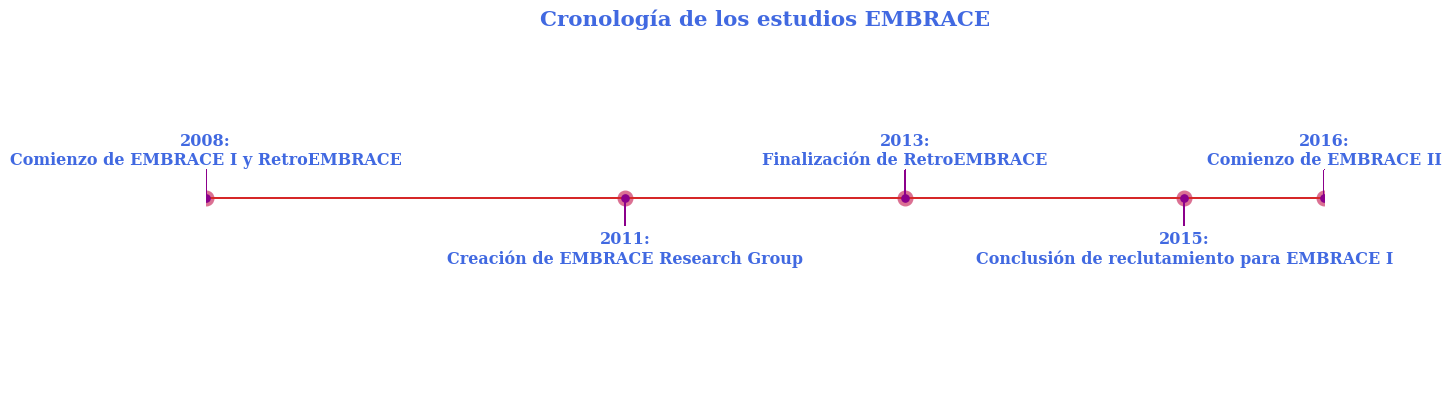
\includegraphics{introduction_files/figure-pdf/fig-embracetimeline-output-1.pdf}

}

\caption{\label{fig-embracetimeline}Línea temporal de EMBRACE}

\end{figure}

El estudio EMBRACE tenía como objetivo recopilar datos de una amplia
cohorte de pacientes tratados con IGBT en entornos mono centricos antes
de su participación en el estudio. Comprende varios estudios, incluidos
los estudios EMBRACEI, RetroEMBRACE y EMBRACEII. El estudio EMBRACEII
incluyó a pacientes con cáncer de cuello uterino avanzado tratadas con
IMRT, quimioterapia y BT guiada por MRI.

El impacto del estudio EMBRACE en la BT para el cáncer de cuello de
útero ha sido significativo. El estudio ha contribuido a mejorar el
control pélvico y la supervivencia en pacientes con cáncer de cuello de
útero localmente avanzado. Ha ayudado a establecer la eficacia de la BT
adaptativa guiada por MRI (HDR-B) para el carcinoma cervical. Los
resultados del estudio han sido comparables a los de otros estudios
multicéntricos, con una toxicidad tardía manejable.

Uno de los principales objetivos del estudio EMBRACEII es reducir la
toxicidad en pacientes que muestran una buena respuesta tras la radio
quimioterapia. El estudio pretende intensificar el tratamiento con BT,
en particular con BT intersticial, para mejorar el control local y la
supervivencia en pacientes con tumores avanzados y mala respuesta
inicial.

A continuación, se enumeran las diferentes fases de EMBRACE

\begin{itemize}
\item
  \textbf{EMBRACE I:} Iniciado en 2008 para evaluar la BT guiada por
  imágenes en un estudio prospectivo multicéntrico. No se establecieron
  restricciones estrictas en la prescripción de dosis para volúmenes
  objetivo u órganos en riesgo. Involucró técnicas intracavitarias e
  intersticiales combinadas. Se reclutaron 1416 pacientes y concluyó en
  2015.
\item
  \textbf{RetroEMBRACE:} Se llevó a cabo simultáneamente a EMBRACE I e
  implicó una recopilación retrospectiva de datos en 12 instituciones.
  Utilizó Recomendaciones Gyn GEC ESTRO para la delimitación de
  objetivos y la presentación de volúmenes de dosis. Recopiló datos de
  instituciones con experiencia clínica previa antes de EMBRACE I. Se
  reclutaron 814 pacientes y se finalizó la recopilación de datos en
  2013.
\item
  \textbf{EMBRACE II:} Iniciado en 2016 con un enfoque en el tratamiento
  local, nodal y sistémico. Prescribe BT adaptativa guiada por MRI con
  restricciones específicas de volumen de dosis. Incluye radioterapia
  externa guiada por imágenes y radioquimioterapia concomitante.
\end{itemize}

\hypertarget{de-las-recomendaciones-de-gec-estro-a-la-icru89}{%
\subsection{De las recomendaciones de GEC-ESTRO a la
ICRU89}\label{de-las-recomendaciones-de-gec-estro-a-la-icru89}}

El proceso de integración de las recomendaciones del GEC ESTRO (I-IV) en
el actual ICRU 89 implicó varios pasos. Inicialmente, en el año 2000, se
creó el Grupo de Trabajo Ginecológico (GWG) del GEC ESTRO con la
participación de médicos y físicos de diferentes centros implicados
activamente en la BT mediante la planificación del tratamiento basada en
imágenes 3D. La tarea del GWG era desarrollar conceptos básicos y un
lenguaje común para comunicar adecuadamente los resultados en el campo
de la BT basada en imágenes 3D. Esto incluía la descripción y el
desarrollo de métodos prácticos para la reconstrucción del aplicador y
la identificación de puntos cruciales en el proceso de reconstrucción.

Un paso más en el proceso fue la creación de la Red Europea de BT
Ginecológica 3D en mayo de 2005, dentro de la cual se definieron varios
proyectos. Uno de estos proyectos se denominó ``Reconstrucción de
aplicadores'' y tenía como objetivo evaluar las incertidumbres
dosimétricas relacionadas con las incertidumbres
geométricas\textsuperscript{\protect\hyperlink{ref-tanderup2008}{40},\protect\hyperlink{ref-hellebust2007}{69}}.

Para facilitar la implementación de estas recomendaciones, se definió un
protocolo detallado, que implicaba la determinación de los parámetros de
consenso con las recomendaciones GYN GEC ESTRO para cada centro dentro
del entorno de tratamiento respectivo para pacientes con diferentes
situaciones clínicas, determinación de objetivos, aplicadores, tasas de
dosis y esquemas de fraccionamiento. Además, el protocolo incluía
directrices para determinar el GTV y el CTV de alto riesgo.

La integración de estas recomendaciones en el actual ICRU 89 supuso una
validación basada en la experiencia clínica y los conceptos dosimétricos
de diferentes instituciones. La adherencia a las recomendaciones se
controló mediante un simulacro y un programa individualizado de garantía
de calidad. Los resultados de los estudios realizados siguiendo estas
recomendaciones mostraron resultados prometedores, incluyendo mejores
tasas de supervivencia, mejor control local y menor aparición de efectos
adversos graves.

\hypertarget{la-inclusiuxf3n-de-la-componente-intersticial}{%
\subsection{La inclusión de la componente
intersticial}\label{la-inclusiuxf3n-de-la-componente-intersticial}}

Una vez adoptado el uso de la MRI y la IGABT, se ha demostrado que la
componente intersticial añadida a la intracavitaria consigue una mayor
conformidad de la dosis y la preservación de los órganos en riesgo.

En Kirisits et
al.\textsuperscript{\protect\hyperlink{ref-kirisits2006a}{70}}
presentaron un aplicador en anillo añadiendo una serie de orificios en
dicho anillo que permite la colocación de agujas, el aplicador Vienna.
Demuestran que el uso de agujas intersticiales adicionales hace que la
dosis prescrita llegue hasta 15 mm en la dirección lateral al punto A,
lo que se traduce en una mejor conformidad mayor. La planificación del
tratamiento basada en un volumen objetivo, restricciones dosis-volumen y
limitaciones para el peso relativo de permanencia de la fuente en las
agujas de la parte intersticial permite aumentar la cobertura de dicho
volumen objetivo sin aumentar la dosis a estructuras a los OAR.

Por otro lado, Nomden et
al.\textsuperscript{\protect\hyperlink{ref-nomden2012}{71}} presentaron
la un estudio clínico del aplicador intersticial compatible MRI/CT, el
aplicador Utrecht, para BT combinada intracavitaria/intersticial en
pacientes con cáncer de cuello de útero. En dicho estudio se muestra la
ganancia dosimétrica en la cobertura del CTV-HR en comparación con el
uso exclusivo de la parte intracavitaria. Esto indica que la adición de
BT intersticial en combinación con BT intracavitaria mejora la
conformidad de la dosis.

También Derks et
al.\textsuperscript{\protect\hyperlink{ref-derks2018}{72}} compararon la
técnica de BT 3D guiada por MRI con la BT 2D convencional, demostrando
la superioridad de la técnica de BT 3D con agujas intersticiales en el
objetivo de lograr un mayor control local y supervivencia en las
pacientes de cáncer de cuello uterino. A la vista de estos resultados se
concluye que la adición de agujas intersticiales, guiadas por MRI,
contribuye a mejorar los resultados del tratamiento.

\hypertarget{sec-esquemadetratamiento}{%
\subsection{Esquema de tratamiento}\label{sec-esquemadetratamiento}}

En el tratamiento del cáncer de cuello uterino localmente avanzado, un
esquema típico implica EBRT pélvica con quimioterapia concurrente
seguida de BT. La EBRT generalmente se administra en dosis de 45 a 50 Gy
en fracciones de 1,8 a 2 Gy, con posibles sobreimpresiones en los
ganglios linfáticos, los parametrios o la pared lateral pélvica,
adaptados al escenario clínico y a la experiencia del centro. El esquema
HDR-BT de 28 Gy en 4 fracciones se ha establecido gracias a los ensayos
EMBRACE, que a menudo se administran en dos aplicaciones durante 1 a 2
semanas, manteniendo un tiempo de tratamiento general por debajo de 50 a
55 días para un control local
óptimo\textsuperscript{\protect\hyperlink{ref-mazeron2015}{73}}.

\hypertarget{prescripciuxf3n-e-informes-de-dosis}{%
\subsection{Prescripción e informes de
dosis}\label{prescripciuxf3n-e-informes-de-dosis}}

Al pasar de una dosimetría 2D a una volumétrica, la prescripción de
dosis ya no tiene sentido hacerla a un punto y se ha de pasar a modos de
prescripción en 3 dimensiones. El histograma dosis-volumen (DVH) es una
herramienta común en la radioterapia externa. Proporciona una
representación gráfica de la distribución de la dosis de radiación
administrada en un tratamiento en función del volumen del tejido
irradiado. Es por ello que parece natural su uso en BT en 3D.

El grupo de trabajo GEC-ESTRO (GYN GEC-ESTRO) introdujo varias métricas
para informar y prescribir dosis basadas en la información suministrada
por los DVH. Las restricciones más habituales son las siguientes:

\begin{itemize}
\item
  \textbf{D90}: El D90 se refiere a la dosis que cubre el 90\% del
  CTV-HR. Es una métrica esencial para evaluar la dosis de radiación
  administrada al área objetivo.
\item
  \textbf{D2cc}: D2cc es la dosis que recibe un volumen específico de un
  OAR. Representa la dosis más alta recibida por un volumen de 2 cc
  (centímetros cúbicos) de OAR. Se ha descubierto que D2cc es valioso
  para evaluar los efectos secundarios tardíos en órganos como la vejiga
  y el recto.
\end{itemize}

\hypertarget{sec-equivalentesbiologicos}{%
\subsection{Equivalentes biológicos}\label{sec-equivalentesbiologicos}}

Como se expuso en la sección~\ref{sec-esquemadetratamiento}, el esquema
habitual de tratamiento incluye varias sesiones de EBRT con fracciones
de 1.8-2 Gy. Dicho fraccionamiento es muy diferente de los que se
utilizan para las fracciones de BT. Ello hace necesario utilizar
equivalentes biológicos que nos permitan sumar la dosis de las
diferentes fases del tratamiento.

Para gestionar la suma de dosis de las fracciones de EBRT y BT, se
recomienda calcular unas dosis biológicamente equivalentes. La suma de
estas dosis representa la dosis total biológicamente ponderada aplicada
al volumen de interés, como la dosis mínima recibida por 2 cc de recto,
el GTV o el CTV-HR.

Como recomienda la
ICRU89\textsuperscript{\protect\hyperlink{ref-ICRU89}{42}} el
equivalente seleccionado es la dosis efectiva en 2Gy por fracción
(EQD2). El EQD2 tiene en cuenta la variación en la sensibilidad a la
radiación de diferentes tejidos y células tumorales, utilizando una
relación alfa/beta (α/β) como medida de radiosensibilidad de los
diferentes tejidos. El valor de α/β normalmente se elige en función del
tipo de tumor que se está tratando. En el caso del cáncer de cuello
uterino, habitualmente se utiliza una relación α/β de 10 para el tumor y
un α/β de 3 Gy para el tejido sano. El EQD2 permite una comparación de
diferentes esquemas de fraccionamiento y ayuda a optimizar los planes de
tratamiento de radiación para lograr los resultados clínicos deseados.
También según las recomendaciones del ICRU89, es la elección para
adecuada para la prescripción de dosis y para los informes de la dosis
recibida por el tumor y por los órganos de riesgo.

Es importante señalar que la integración de nuevos parámetros y el uso
de herramientas tridimensionales para la evaluación del volumen de dosis
deben usarse de manera prospectiva para la evaluación a corto y largo
plazo, con el fin de establecer información clínica valiosa
correlacionada con las relaciones de volumen de dosis en 3D. Además, se
deben integrar métodos apropiados para la evaluación de la morbilidad
para diferentes sistemas de órganos. Durante un período de transición,
estas herramientas 3D deben usarse en paralelo con puntos de referencia
basados en películas como proponía el ICRU 38 y otros puntos propuestos
en la literatura, como el punto máximo de la vejiga, el punto medio y
máximo del recto,
etc\textsuperscript{\protect\hyperlink{ref-srivastava2014}{74}--\protect\hyperlink{ref-kim2007}{77}}.

\hypertarget{reconstrucciuxf3n-de-aplicadores}{%
\section{Reconstrucción de
aplicadores}\label{reconstrucciuxf3n-de-aplicadores}}

\hypertarget{aplicadores-en-bt}{%
\subsection{Aplicadores en BT}\label{aplicadores-en-bt}}

Un aplicador de BT es un dispositivo que se utilizado para administrar
radiación directamente al tumor o tejido objetivo. Está diseñado para
sostener y colocar las fuentes radiactivas muy cerca del área de
tratamiento, lo que permite una administración de radiación precisa y
controlada. El aplicador garantiza que la radiación se administre con
una dosis alta al tumor y al mismo tiempo minimiza la exposición a la
radiación de los tejidos sanos circundantes.

Los aplicadores utilizados en BT deben estar aprobados y marcados para
su uso clínico que requiere de interacción entre fabricantes y clientes
con el objetivo de diseñar aplicadores con características específicas
para cada zona de tratamiento. Hay diferentes tipos de aplicadores
disponibles para diversas áreas de tratamiento, como ginecología,
bronquios y mamas. En el caso ginecológico se utilizan canales por donde
circula la fuente fabricados en plástico o titanio. La elección de estos
materiales no es arbitraria, ya que ambos materiales son compatibles con
equipos de MR.

\hypertarget{sec-tiposreconstruccion}{%
\subsection{Tipos de reconstrucción}\label{sec-tiposreconstruccion}}

La reconstrucción del aplicador implica identificar con precisión la
ruta de la fuente dentro de los catéteres y el aplicador, lo cual es
esencial para calcular la dosis administrada al objetivo y a los órganos
en riesgo. Implica el uso de modalidades de imágenes, como el CT o la
radiografía, para reconstruir la posición de fuentes radiactivas o
aplicadores dentro del cuerpo del paciente. El objetivo es garantizar
que la ubicación real de las fuentes o aplicadores coincida con la
ubicación planificada en el sistema de planificación del tratamiento
(TPS). De no ser que se mencione lo contrario, se asumirá que la
reconstrucción se hace sobre conjuntos de imágenes tridimensionales.
Existen diferentes dos diferentes enfoques para la reconstrucción del
aplicador: La reconstrucción directa y las bibliotecas de aplicadores.

El método de reconstrucción directa se basa en el uso de maniquíes
llenos de sustancias que producen una señal de alta intensidad
(\emph{dummies}). Estas \emph{dummies} hacen visible la trayectoria de
la fuente dentro del aplicador. Sin embargo, la eficacia de este método
depende de la disponibilidad de \emph{dummies} que puedan producir una
señal visible en la modalidad de imagen elegida.

El objetivo principal de las \emph{dummies} es proporcionar una
referencia o marcador para que los físicos médicos determinen con
precisión la posición y orientación de los aplicadores o catéteres
dentro del cuerpo del paciente. Al utilizar maniquíes, el proceso de
planificación del tratamiento se vuelve más preciso y fiable.

Cuando la modalidad de imagen es CT, se deben utilizan maniquíes
construídos a partir de materiales compuestos de materiales de alto
número atómico para que sean fácilmente visibles. Es importante que
dichas \emph{dummies} no produzcan artefactos en la imagen que
dificulten la reconstrucción o la segmentación del tumor y los OAR. La
cuestión es que como se ha visto en párrafos anteriores, la modalidad de
imagen ideal en BT de cérvix es la imagen por resonancia magnética
nuclear.

La reconstrucción directa sobre MRI requiere del uso de \emph{dummies}
específicas visibles en
MRI\textsuperscript{\protect\hyperlink{ref-perez-calatayud2009}{78}}. La
señal producida por la \emph{dummy} representa la trayectoria de la
fuente de radiación dentro del aplicador, al igual que se vio en el caso
de CT. Sin embargo, a veces no es fácil construir \emph{dummies} para
aplicadores con diámetros de canal pequeños o componentes intersticiales
donde la señal producida por el maniquí es demasiado débil. Además, en
el caso de aplicadores de titanio, dicho material enmascara la señal de
una \emph{dummy} construida con sustancias visibles en MRI.

Siguiendo con los aplicadores y agujas de titanio, pueden producirse
artefactos en la imagen cuando se utilizan sobre MRI. Los aplicadores y
agujas de titanio crean una señal de vacío en la resonancia magnética,
lo que dificulta determinar la ruta de la fuente dentro de
ellos\textsuperscript{\protect\hyperlink{ref-richart2018}{34}}. Además,
se pueden inducir artefactos de susceptibilidad y abombamiento en el
extremo del aplicador y las agujas. Estos artefactos complican aún más
la identificación precisa de la trayectoria de la fuente.

Por otro lado, existe la cuestión de la determinación de la primera
posición de parada (\emph{tip position}).

El concepto de primera posición de parada se refiere a la ubicación de
la punta de un aplicador o aguja utilizada en la planificación del
tratamiento de BT para el cáncer de cuello uterino. La determinación
precisa de la posición de la punta es crucial para la planificación y el
resultado adecuados del tratamiento. Garantiza que las posiciones de
parada de las fuentes de radiación estén determinadas correctamente,
minimizando las imprecisiones en la distribución de dosis. Una posición
incorrecta de la punta puede provocar una administración de dosis
incorrecta y potencialmente comprometer la eficacia del tratamiento.

En el caso de poner en servicio un aplicador nuevo, la posición de la
punta se verifica y mide en relación con la superficie exterior del
aplicador o puntos de referencia dentro del
aplicador\textsuperscript{\protect\hyperlink{ref-hellebust2010}{61}}.
Por ejemplo, la distancia desde la punta de un aplicador o aguja en
tándem hasta la primera posición de parada se determina durante la
puesta en servicio. De manera similar, la distancia desde la parte
superior de un aplicador de anillo hasta el nivel del camino de la
fuente también es importante para ubicar el punto A en relación con el
aplicador.

También la determinación de la posición de la punta en la reconstrucción
de aplicadores puede verse afectada por el espesor de corte de las
imágenes de resonancia magnética. Un espesor de corte más pequeño,
normalmente alrededor de 3-4 mm, puede provocar incertidumbres al
determinar el extremo de la punta de los canales de la fuente. Esta
inexactitud se puede reducir mediante el uso de secuencias de imágenes
adicionales, como parasagital o 3D, pero la adición de nuevas secuencias
introduce nuevos focos de incertidumbre.

\hypertarget{sec-bibapp}{%
\subsection{Bibliotecas de aplicadores}\label{sec-bibapp}}

Otro enfoque para la reconstrucción del aplicador es el uso de
bibliotecas de aplicadores. Las bibliotecas de aplicadores son un
concepto utilizado en el proceso de reconstrucción de la geometría del
aplicador en la planificación del tratamiento de BT basada en imágenes
3D. Consisten en modelos 3D precisos y predefinidos de diferentes tipos
de aplicadores utilizados en procedimientos de BT. Estas bibliotecas se
utilizan para importar la configuración del aplicador al TPS y hacerla
coincidir con la señal producida por el aplicador en las imágenes de
resonancia
magnética\textsuperscript{\protect\hyperlink{ref-hellebust2010}{61}}.

Las ventajas de las bibliotecas de aplicadores sobre los métodos de
reconstrucción directa son significativas en el caso de reconstrucción
exclusiva sobre MRI. En primer lugar, el uso de bibliotecas de
aplicadores permite un proceso de reconstrucción rápido y sencillo. El
modelo de aplicador importado se puede trasladar y rotar hasta que
coincida con la señal de producida por el aplicador real, lo que
proporciona una verificación visual de la reconstrucción del aplicador.
Esto minimiza el riesgo de introducir una geometría incorrecta del
aplicador durante el proceso de reconstrucción.

Además, el uso de bibliotecas de aplicadores reduce la probabilidad de
errores e incertidumbres en la reconstrucción. Dado que el modelo 3D del
aplicador está representado con precisión en la biblioteca, la
verificación visual puede garantizar que la señal de vacío del aplicador
coincida con la forma modelada del aplicador. Esto asegura que el
proceso de reconstrucción sea más confiable y minimiza los errores
sistemáticos en la distribución de dosis durante la planificación del
tratamiento.

Sin embargo, existen limitaciones en el uso de bibliotecas de
aplicadores. En primer lugar, este método sólo es viable para
aplicadores rígidos. Los aplicadores flexibles o ajustables pueden
requerir una reconstrucción independiente de cada parte debido a
posibles desviaciones de la forma modelada del aplicador durante la
inserción en el paciente.

Además, la disponibilidad de bibliotecas de aplicadores depende del
sistema de planificación del tratamiento que se utilice. Si bien algunos
sistemas TPS tienen una biblioteca de aplicadores disponibles, es
posible que otros no proporcionen esta funcionalidad. Además, los
métodos para fusionar el sistema de coordenadas del archivo de la
biblioteca con el sistema de coordenadas del estudio clínico 3D pueden
variar según el sistema de planificación del tratamiento. Esto introduce
posibles desafíos e incertidumbres en el proceso de
reconstrucción\textsuperscript{\protect\hyperlink{ref-hellebust2010}{61}}.

Por otro lado, el uso de bibliotecas de aplicadores puede contribuir a
minimizar el problema de la determinación de posición de la punta ya que
dichas bibliotecas contienen modelos 3D precisos del aplicador. Al
importar la configuración del aplicador correspondiente de la biblioteca
al TPS y alinearla con la señal de anulación, en otras palabras, la
sombra negra que deja el aplicador en la imagen, producida por la misma
en la MRI, no es necesario ver explícitamente la punta del aplicador.

\hypertarget{sec-pv}{%
\section{Planes virtuales}\label{sec-pv}}

El objetivo del aplicador Benidorm (Lorca Marin, Murcia, Spain) para BT
intersticial es proporcionar un nuevo aplicador de BT para tumores
ginecológicos, en particular para el carcinoma cervical localmente
avanzado\textsuperscript{\protect\hyperlink{ref-villalba2015}{79}}. Este
aplicador combina la radioterapia intracavitaria con agujas
intersticiales transperineales compatibles con MR, intentando superar
las limitaciones de las plantillas de agujas actualmente disponibles en
el mercado. Permite la cobertura total de la extensión craneocaudal y
lateral del tumor, incluyendo las regiones intrauterinas, parametriales
y paravaginales. El aplicador Benidorm (figura~\ref{fig-tb}) está
indicado principalmente para casos de carcinoma cervical avanzado con
invasión parametrial voluminosa, afectación paravaginal extensa o
invasión de la vejiga o el recto. Su diseño permite mejorar el contorno
y la planificación conformada del tratamiento basándose únicamente en la
MR.

\begin{figure}

{\centering 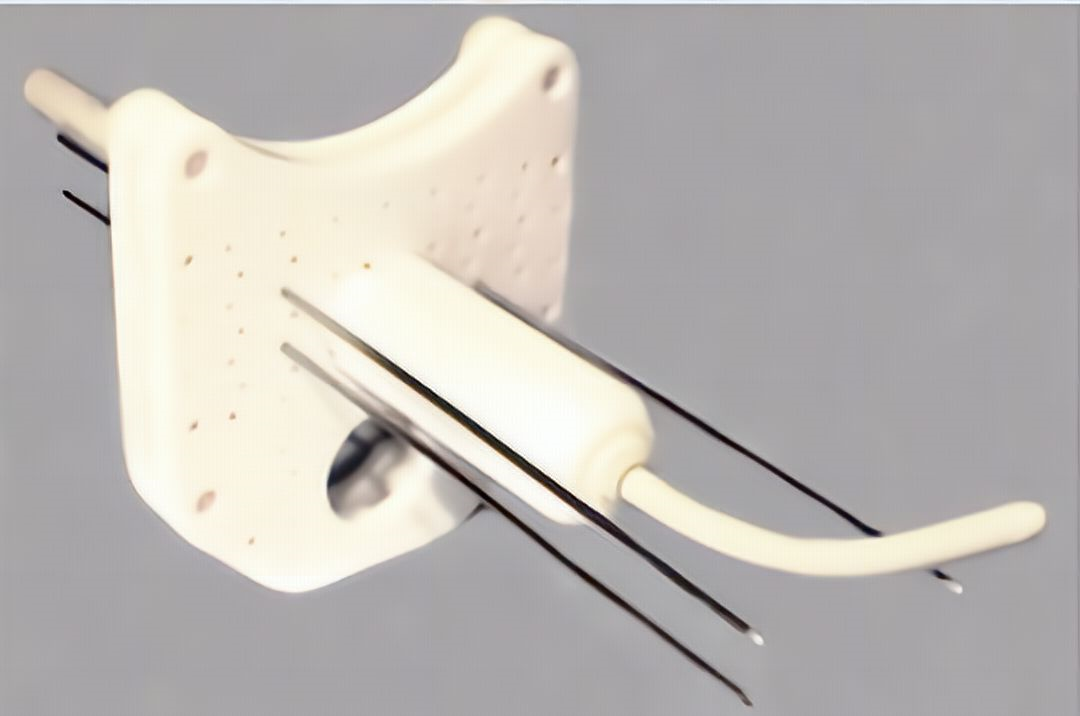
\includegraphics{img/TB.png}

}

\caption{\label{fig-tb}Vista del aplicador Benidorm}

\end{figure}

Consta de una plantilla con orificios rectos y angulados que permiten la
inserción de agujas de titanio en con diferente divergencia, junto con
los tubos intrauterinos compatibles con MR existentes en la actualidad.
Dispone de 12 filas de orificios, con 35 orificios rectos y 16 orificios
divergentes (\(7^{\circ}\)), ofreciendo la posibilidad de una cobertura
total de la extensión del tumor, incluyendo el parametrio distal y toda
la vagina. El aplicador también permite la inclusión de un cilindro
vaginal y dispone de pistas obturadoras de plástico para evitar el
desplazamiento de la aguja. En resumen, el aplicador Benidorm combina
las ventajas de los aplicadores MUPIT y Utrecht y permite una
planificación exclusiva basada en MR para el tratamiento de BT.

La configuración de agujas del aplicador Benidorm dota de una gran
flexibilidad en la elección de agujas a implantar para cubrir el volumen
objetivo. Por otro lado, para corregir la posible desviación de la aguja
de su posición óptima puede hacer necesaria la necesidad de inserciones
repetidas para su colocación en el sitio previsto. Estas inserciones
repetidas de agujas pueden contribuir a aumentar el traumatismo de los
tejidos circundantes. Cada inserción puede causar una deformación y un
traumatismo adicionales en los tejidos, lo que puede provocar molestias
o dolor a la paciente e incidir negativamente en su recuperación post
operatoria.

Es por ello que diseñar un tratamiento con el mínimo número de agujas
que a su vez asegure la cobertura correcta del volumen objetivo.

\hypertarget{objetivos}{%
\section{Objetivos}\label{objetivos}}

La primera
publicación\textsuperscript{\protect\hyperlink{ref-otal2017}{80}}
presenta un método para añadir la componente intersticial a una librería
de aplicadores rígidos en el entorno Oncentra, en el caso del aplicador
Utrecht existente y la adición de un aplicador nuevo completo,
permitiendo así una reconstrucción más eficiente utilizando la
planificación exclusiva sobre MRI.

El segundo artículo
publicado\textsuperscript{\protect\hyperlink{ref-rodriguez2017}{81}}
presenta la implementación de una técnica de planificación virtual
pre-plan para el aplicador Benidorm en BT ginecológica multi
intersticial, tanto transperineal como endocavitaria.

El tercer trabajo\textsuperscript{\protect\hyperlink{ref-otal2022}{82}}
es una revisión de las diferentes metodologías utilizadas por todos los
TPS disponibles comercialmente para resolver los principales problemas
de planificación en una BT de cérvix basada exclusivamente en RM con
tratamiento de componentes intersticiales. Además, se esbozan algunos
aspectos prácticos deseables o convenientes de implementar en futuras
versiones de TPS desde las perspectivas del oncólogo radioterapeuta y
del físico médico.

\bookmarksetup{startatroot}

\hypertarget{material-y-muxe9todos}{%
\chapter{Material y métodos}\label{material-y-muxe9todos}}

\hypertarget{a-method-to-incorporate-interstitial-components-into-the-tps-gynecologic-rigid-applicator-library-otal2017-publicado-en-febrero-de-2017}{%
\section{A method to incorporate interstitial components into the TPS
gynecologic rigid applicator library (Otal2017 publicado en febrero de
2017)}\label{a-method-to-incorporate-interstitial-components-into-the-tps-gynecologic-rigid-applicator-library-otal2017-publicado-en-febrero-de-2017}}

\hypertarget{sec-appimagestps}{%
\subsection{Aplicadores, adquisición de imágenes de resonancia magnética
y planificador de braquiterapia (TPS)}\label{sec-appimagestps}}

El aplicador Utrecht compatible con CT y MR (Nucletron, una empresa de
Elekta, Elekta AB, Estocolmo, Suecia) se desarrolló específicamente para
el tratamiento combinado intracavitario/intersticial de cánceres
ginecológicos\textsuperscript{\protect\hyperlink{ref-nomden2012}{71}}.
Su diseño se basa en el aplicador Fletcher (Nucletron, una compañía de
Elekta, Elekta AB, Estocolmo, Suecia), utilizando los ovoides como
plantilla para la colocación de agujas intersticiales (hasta 5 agujas de
plástico en cada uno). La profundidad de inserción de las agujas puede
controlarse mediante una herramienta suministrada por el fabricante
figura~\ref{fig-utrecht_tool}. La colocación final de las agujas depende
del implante, tanto en trayectoria como en profundidad. Sin embargo,
aunque existen \emph{dummies} para el componente endocavitario, no los
hay para el intersticial. Hasta ahora, las posiciones de las agujas se
reconstruían utilizando su señal de túnel negro en MR T2 y la medida de
la profundidad de inserción.

\begin{figure}

\begin{minipage}[t]{0.50\linewidth}

{\centering 

\raisebox{-\height}{

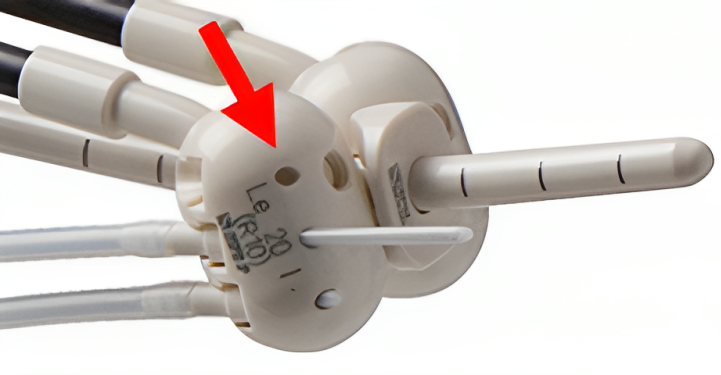
\includegraphics{img/Utrecht_tool1.png}

}

}

\subcaption{\label{fig-utrecht_tool1}Detalle de la profundidad de
inserción sobre el aplicador}
\end{minipage}%
%
\begin{minipage}[t]{0.50\linewidth}

{\centering 

\raisebox{-\height}{

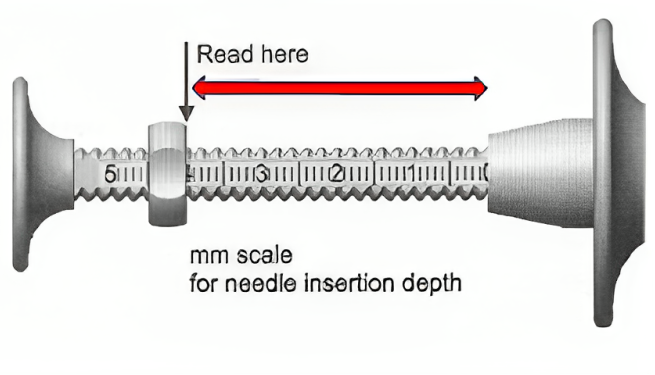
\includegraphics{img/Utrecht_tool2.png}

}

}

\subcaption{\label{fig-utrecht_tool2}Herramienta de inserción}
\end{minipage}%

\caption{\label{fig-utrecht_tool}Procedimiento de medida de la inserción
de las agujas}

\end{figure}

El aplicador Benidorm (TB) (Lorca Marín, Murcia, España) consiste en una
plantilla para guíar múltiples agujas de titanio y un cilindro en cuyo
centro se coloca una sonda
intrauterina\textsuperscript{\protect\hyperlink{ref-villalba2015}{79},\protect\hyperlink{ref-richart2015}{83}}
(figura~\ref{fig-tbimage}). Esta plantilla es una actualización de la
plantilla existente
MUPIT\textsuperscript{\protect\hyperlink{ref-gynecolo2011}{84}}
(Nucletron, una empresa de Elekta, Elekta AB, Estocolmo, Suecia) a la
que añade un componente intracavitario, la sonda intrauterina, y la hace
completamente compatible con MR. La plantilla consta de dos placas
perineales con dos orificios centrales que permiten la colocación de un
cilindro vaginal, disponible en diferentes tamaños para adaptarse a
diferentes longitudes vaginales y tubos intrauterinos de ángulos y
longitudes variables. Además, las placas están perforadas con orificios
para introducir agujas de titanio rectas y
anguladas\textsuperscript{\protect\hyperlink{ref-richart2015}{83}}. Las
placas tienen tres alojamientos en los que se colocan tres bolas de
vitamina A. Estas bolas producen una señal de excelente visibilidad en
las secuencias T1 y T2 de la MRI y su presencia obedece a ayudar en el
proceso de reconstrucción. Las agujas se reconstruyen siguiendo la señal
del túnel negro y el vacío de la punta. En la MR en T1, las posiciones
pueden determinarse correctamente, pero en T2 el contraste es
insuficiente\textsuperscript{\protect\hyperlink{ref-richart2015}{83}}.
Por lo tanto, la profundidad de inserción de cada aguja ha de obtenerse
midiendo la longitud libre con una regla.

\begin{figure}

{\centering 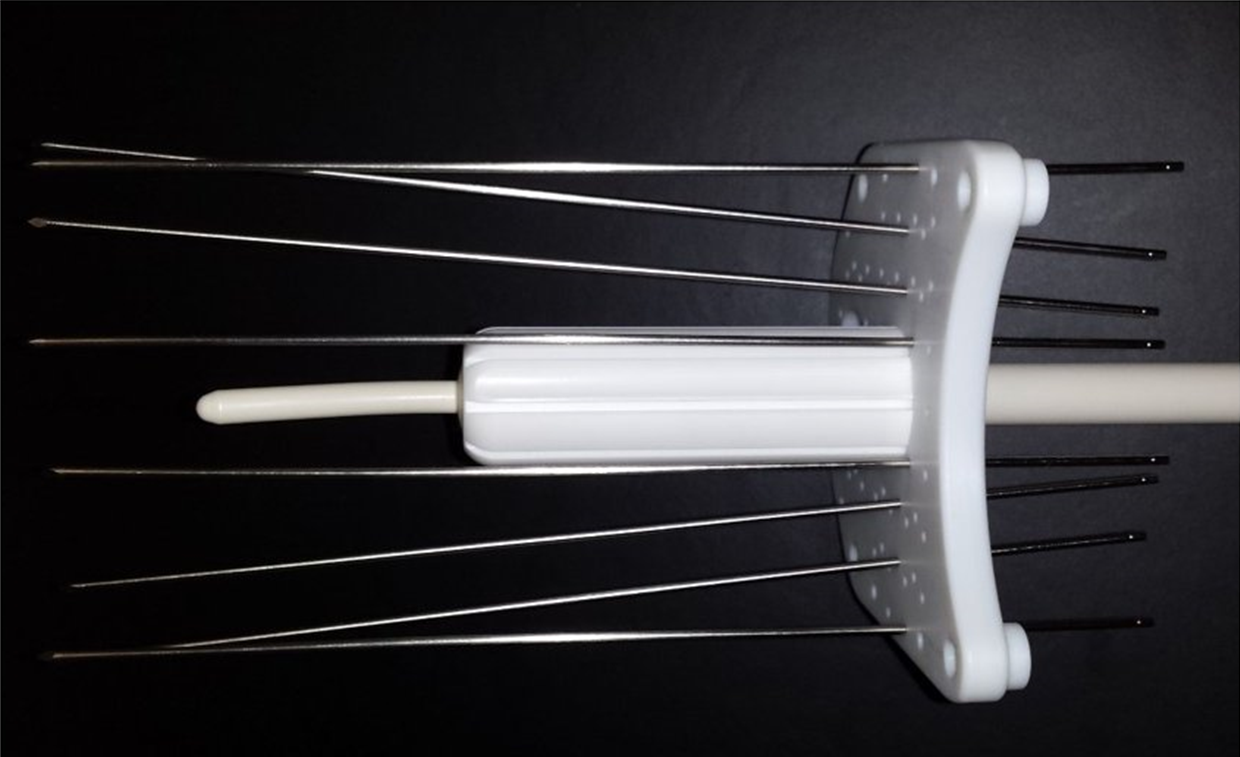
\includegraphics{img/TBfoto.png}

}

\caption{\label{fig-tbimage}aplicador Benidorm}

\end{figure}

Las exploraciones de MR de los pacientes se adquirieron con un generador
de imágenes de MR de 1,5 T (Optima MR 450w, software versión DV24, GE
Medical Systems, Milwaukee, Wisconsin, EE.UU.). Se utilizó una bobina
receptora \emph{phased array} de ocho canales siguiendo los protocolos
clínicos de MR estándar. Siguiendo las recomendaciones de
GEC-ESTRO\textsuperscript{\protect\hyperlink{ref-haie-meder2005}{20},\protect\hyperlink{ref-viswanathan2012}{47},\protect\hyperlink{ref-potter2006}{60}},
la adquisición consistió en una secuencia axial de eco espín rápido con
recuperación rápida ponderada en T2 (FRFSE) con un grosor de corte
reducido a 2 mm. Esta secuencia se utilizó tanto para el contorneo como
para la reconstrucción. Los detalles de la configuración de adquisición
de imágenes de resonancia magnética están descritos en la publicación de
Richart et al.\textsuperscript{\protect\hyperlink{ref-richart2015}{83}}.
La biblioteca desarrollada se ha implementado en el Oncentra
Brachytherapy TPS (Nucletron, una empresa de Elekta, Elekta AB,
Estocolmo, Suecia), versión 4.3.0, con un módulo de braquiterapia que
incluye una biblioteca de aplicadores rígidos. Se utilizó un programa
independiente, el \emph{Library Manager Applicator} (LMA), para añadir
modelos 3D de los aplicadores a la base de datos de Oncentra.

\hypertarget{modelizaciuxf3n-de-los-aplicadores-utrecht-y-aplicador-benidorm-en-la-biblioteca-de-aplicadores-de-oncentra}{%
\subsection{Modelización de los aplicadores Utrecht y aplicador Benidorm
en la biblioteca de aplicadores de
Oncentra}\label{modelizaciuxf3n-de-los-aplicadores-utrecht-y-aplicador-benidorm-en-la-biblioteca-de-aplicadores-de-oncentra}}

En el Oncentra Brachytherapy TPS, los archivos de entrada para el gestor
de la biblioteca de aplicadores son un conjunto de archivos Extensible
Markup Language (xml) organizados en una estructura jerárquica. El
archivo principal tiene una extensión \emph{rule.xml}. En este archivo
principal se configura cada aplicador, con todas sus opciones, para su
uso en Oncentra. Los bloques utilizados en este archivo son archivos
independientes que incluyen información sobre las propiedades de los
canales, ovoides, etc. Estos bloques se dividen en cuatro tipos de
ficheros: tubos, ovoides, cilindros y fijaciones. Estos ficheros
contienen cuatro subsecciones: 1- Una descripción del fichero, que
incluye el ID de la pieza y el tipo. 2- El conjunto de puntos de
anclaje. 3- Los conectores utilizados. 4- Información sobre la
superficie del elemento (llamada \emph{skin} en Oncentra).

\hypertarget{sec-apputrecht}{%
\subsection{El aplicador Utrecht}\label{sec-apputrecht}}

En este caso, se parte de un modelo proporcionado por Elekta sin la
componente intersticial. El primer paso es determinar la distancia desde
la superficie de los ovoides de los puntos de salida de las agujas. Se
utilizó la información técnica facilitada por Elekta para obtener las
coordenadas de los puntos de salida de las agujas en el sistema de
referencia intrínseco de los ovoides (figura~\ref{fig-esquemautrecht}).
Para determinar las coordenadas en el sistema de referencia del
aplicador, se ha de encontrar la traslación y rotación necesarias. La
traslación viene dada por la posición de la punta de cada canal del
ovoide. Para hallar la rotación, se obtuvo el plano que contiene cada
uno de los canales de los ovoides a partir de los datos del archivo
correspondiente utilizando un método de mínimos cuadrados. Una vez
definidos los planos, se hace coincidir las direcciones x y z en ambos
sistemas de referencia.

\begin{figure}

{\centering 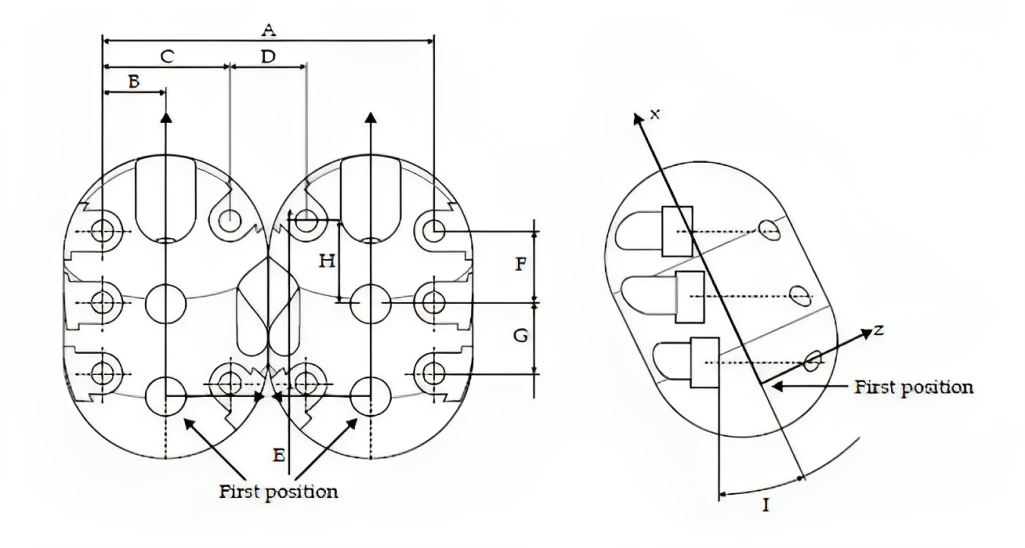
\includegraphics{img/Esquema_utrecht.PNG}

}

\caption{\label{fig-esquemautrecht}Sistema de referencia intrínseco del
ovoide obtenido de la documentación técnica de Elekta}

\end{figure}

Una obtenidos los puntos de salida, el siguiente paso es crear un
archivo correspondiente a cada aguja. Se creó un modelo 3D de cada aguja
con FreeCAD (versión 0.14, http://www.freecadweb.org/) y el software
Open Parametric Modeler. Exportando este modelo a un archivo .obj de
Wavefront y procesándolo en Excel, obtuvimos la sección \emph{skin}. El
conector de la aguja en este nuevo archivo también se obtuvo utilizando
un modelo de FreeCAD. Los conectores definidos en el archivo del canal
del ovoide son los puntos de salida del ovoide calculados en el sistema
de referencia del aplicador Utrecht.

\hypertarget{sec-templatebenidorm}{%
\subsection{El aplicador Benidorm}\label{sec-templatebenidorm}}

El proceso de modelado para el TB fue diferente. Dado que en la base de
datos de Oncentra sólo se incluían los tubos intrauterinos del conjunto
de aplicadores vaginales, se utilizó FreeCAD para crear un nuevo modelo
3D del \emph{template}. Con este programa, fue convertido el diseño real
a un archivo vectorial se modelaron las agujas de titanio con un proceso
análogo al descrito en la sección~\ref{sec-apputrecht}, los 4 cilindros
(45 mm, 80 mm, 100 mm y 135 mm) y las placas perineales con las esferas
de vitamina A (figura~\ref{fig-tbfreecad}). Mediante este paso se
obtiene la información necesaria sobre el \emph{skin} del aplicador, y
se encuentran los datos necesarios para obtener las posiciones relativas
de todas las partes que configuran el aplicador, de forma que se puedan
crear los conectores. Toda esta información permite la creación de los
diferentes archivos y sus enlaces utilizando técnicas descritas en la
sección~\ref{sec-apputrecht}.

\begin{figure}

{\centering 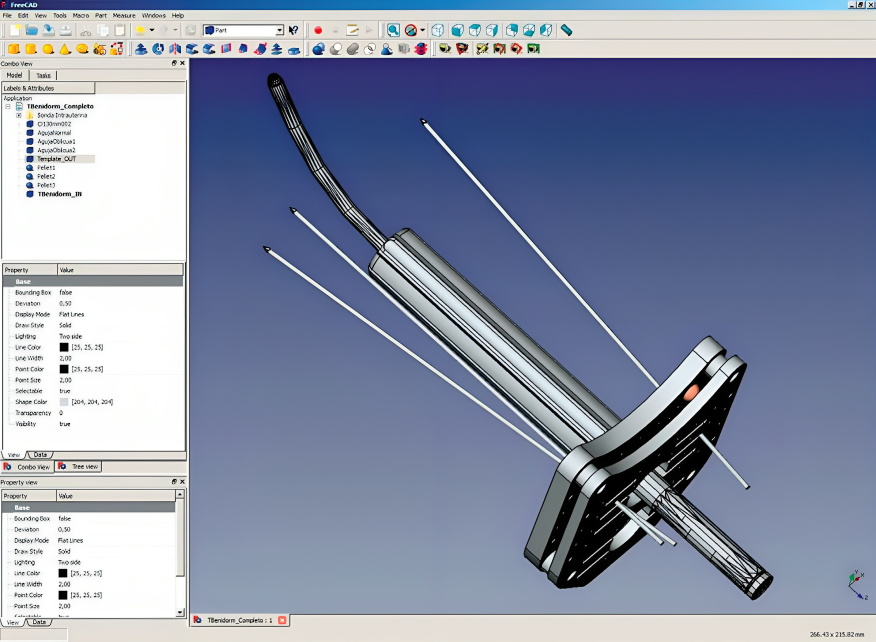
\includegraphics{img/TB_freecad.png}

}

\caption{\label{fig-tbfreecad}Modelo del aplicador Benidorm en FreeCAD}

\end{figure}

\hypertarget{sec-MM-reconstruction}{%
\subsection{Procedimiento de
reconstrucción}\label{sec-MM-reconstruction}}

En el caso del aplicador de Utrecht, el proceso de reconstrucción de la
MR T2 se basó en los puntos que tienen en común la sección rígida y la
parte intersticial. En primer lugar, la parte rígida se reconstruye
utilizando las \emph{dummies} específicas que existen para la sonda
intrauterina y los ovoides, que son claramente visibles en la secuencia
T2, junto con el \emph{skin} del aplicador. Estos se han descrito en una
publicación
anterior\textsuperscript{\protect\hyperlink{ref-perez-calatayud2009}{78}}
y las \emph{dummies} son comercializadas por la compañía Elekta. Estas
\emph{dummies} consisten en catéteres llenos de una mezcla de solución
salina y yodo. El agua es la que proporciona la visibilidad en la
imagen, y el yodo simplemente colorea el líquido para facilitar la
comprobación de la presencia de burbujas. El extremo distal del maniquí
se corresponde con la primera posición de parada de la fuente (\emph{tip
position}). La posición de la punta de ambos ovoides y la posición de la
punta del tándem intrauterino (marcadores de MRI) se utilizan como
puntos de referencia para localizar el aplicador. Se realizan pequeñas
correcciones para ajustar mejor el canal negro dejado por el aplicador y
los marcadores de MRI, utilizando las marcas de la \emph{skin} de los
ovoides y la sonda. A diferencia de la sonda y los ovoides, este tipo de
\emph{dummies} son incompatibles con las agujas de plástico, debido a su
diámetro más estrecho. Puede haber ligeras desviaciones de las
posiciones modeladas de las puntas de las agujas. Para ajustar las
agujas a su posición en el implante, pueden realizarse pequeñas
correcciones girando las agujas alrededor de los puntos de salida en los
ovoides.

La modelización correcta de la componente intracavitaria nos da la
localización de los puntos de salida de las agujas, es decir, los puntos
de salida en la superficie del ovoide. Combinando esta información con
la longitud libre, nos permite conocer la posición completa de la aguja.
En el caso del TB, una vez hecha la elección de las agujas, se introduce
la configuración de las agujas y los datos de la longitud libre en una
aplicación java programada por los autores para generar archivos xml y
posteriormente se importa en la biblioteca de aplicadores.

\hypertarget{pre-plan-technique-feasibility-in-multi-interstitialendocavitary-perineal-gynecological-brachytherapy-rodriguez2017-publicado-en-octubre-2017}{%
\subsection{Pre-plan technique feasibility in
multi-interstitial/endocavitary perineal gynecological brachytherapy
(Rodriguez2017 publicado en octubre
2017)}\label{pre-plan-technique-feasibility-in-multi-interstitialendocavitary-perineal-gynecological-brachytherapy-rodriguez2017-publicado-en-octubre-2017}}

La descripción del aplicador Benidorm, el procedimiento de adquisición y
el modelado en la biblioteca de aplicadores de Oncentra ya se describió
en la sección~\ref{sec-appimagestps}.

El procedimiento de pre-planificación implementado es el siguiente:

\begin{enumerate}
\def\labelenumi{\arabic{enumi}.}
\item
  La adquisición de MR T2 previa a la braquiterapia se realiza con la
  plantilla colocada sólo con el cilindro vaginal (sin sonda uterina ni
  agujas) 3-5 días antes del implante de braquiterapia. Se introduce un
  obturador vaginal de longitud conocida (40, 60, 100 o 130 mm según la
  longitud vaginal) y se llena la vejiga con 50 cc de solución salina.
\item
  En este conjunto de imágenes, se dibuja el CTV. El volumen diana (GTV)
  clínico y de imagen en el momento del diagnóstico y el GTV en el
  momento de la braquiterapia se unifican en un único CTV, incluyendo
  GTV, CTV-HR y CTV de riesgo intermedio (CTV-IR), basándose en las
  recomendaciones del GEC
  ESTRO\textsuperscript{\protect\hyperlink{ref-viswanathan2007}{33},\protect\hyperlink{ref-gynecolo2011}{84},\protect\hyperlink{ref-yoshida2010}{85}}.
  Las agujas necesarias y sus profundidades se seleccionan para abarcar
  el CTV (de la forma más conforme posible). Para facilitar esta tarea,
  se ha desarrollado una aplicación basada en Java vinculada al TPS
  (Oncentra Prostate versión 4.3, Elekta AB, Estocolmo, Suecia). A
  partir de este procedimiento, se obtiene la identificación de cada
  aguja y su profundidad previamente al implante.
\item
  Con esta información, el oncólogo radioterapeuta procede al implante
  y, posteriormente, se realiza una resonancia magnética post-implante,
  en la que se establece el contorno, las agujas más la reconstrucción
  en tándem, y la optimización.
\end{enumerate}

\hypertarget{review-on-treatment-planning-systems-for-cervix-brachytherapy-interventional-radiotherapy-some-desirable-and-convenient-practical-aspects-to-be-implemented-from-radiation-oncologist-and-medical-physics-perspectives-otal2022-publicado-en-julio-2022}{%
\section{Review on Treatment Planning Systems for Cervix Brachytherapy
(Interventional Radiotherapy): Some Desirable and Convenient Practical
Aspects to Be Implemented from Radiation Oncologist and Medical Physics
Perspectives (Otal2022 publicado en julio
2022)}\label{review-on-treatment-planning-systems-for-cervix-brachytherapy-interventional-radiotherapy-some-desirable-and-convenient-practical-aspects-to-be-implemented-from-radiation-oncologist-and-medical-physics-perspectives-otal2022-publicado-en-julio-2022}}

Los autores de esta revisión son oncólogos radioterápicos y físicos
médicos con amplia experiencia en tratamientos de braquiterapia HDR de
cérvix con componente intersticial basados en MR, representantes de los
centros españoles con mayor número de implantes realizados. Los tres TPS
analizados fueron Brachyvision v16.0 de Varian (Varian Medical Systems,
Palo Alto, CA, USA), Oncentra v4.6.2 de Elekta (Elekta AB, Estocolmo,
Suecia), y Sagiplan v2.2 de BEBIG (Eckert \& Ziegler BEBIG GmbH, Berlín,
Alemania). La mayoría de los autores son usuarios de Oncentra Brachy,
con un solo usuario de Brachyvision; no hay usuarios de Sagiplan. Al ser
un grupo multidisciplinar se impone el especificar la contribución de
cada uno de los autores, apareciendo esta en el artículo original.

Las revisiones de los TPS se basaron en la experiencia clínica de los
autores y en demostraciones interactivas proporcionadas por los
fabricantes de los TPSs. En estas demostraciones, la versión de TPS
probada fue la última disponible comercialmente, incluyendo también
todas las nuevas herramientas actualmente desarrolladas para ser
incluidas en futuras versiones. Tras una introducción a la mayoría de
las utilidades y herramientas de los sistemas de planificación, se pidió
al especialista de la empresa vendedora (en adelante, especialista) que
respondiera a algunas de las cuestiones que se plantean habitualmente en
un entorno clínico y que se describirán brevemente a continuación. Con
el fin de seguir un enfoque sistemático en la evaluación de las
capacidades de cada TPS, se realizaron demostraciones basadas en el
cuestionario resumido en la tabla~\ref{tbl-cuestionario}. También se
preguntó a los especialistas sobre software externo. También se preguntó
a los especialistas sobre programas y dispositivos externos disponibles
comercialmente o en fase de desarrollo que pudieran arrojar alguna luz
sobre estos problemas.

\hypertarget{tbl-cuestionario}{}
\begin{longtable}[]{@{}
  >{\raggedright\arraybackslash}p{(\columnwidth - 2\tabcolsep) * \real{0.1806}}
  >{\raggedright\arraybackslash}p{(\columnwidth - 2\tabcolsep) * \real{0.8194}}@{}}
\caption{\label{tbl-cuestionario}El cuestionario presentado a cada uno
de los especialistas}\tabularnewline
\toprule\noalign{}
\begin{minipage}[b]{\linewidth}\raggedright
Pregunta
\end{minipage} & \begin{minipage}[b]{\linewidth}\raggedright
Descripción
\end{minipage} \\
\midrule\noalign{}
\endfirsthead
\toprule\noalign{}
\begin{minipage}[b]{\linewidth}\raggedright
Pregunta
\end{minipage} & \begin{minipage}[b]{\linewidth}\raggedright
Descripción
\end{minipage} \\
\midrule\noalign{}
\endhead
\bottomrule\noalign{}
\endlastfoot
Q1 & Herramientas de puesta en marcha y control de calidad. \\
Q2 & Registro de imágenes y utilidades para gestionar información de
tratamientos previos. \\
Q3 & Contorneo en MRI. Eliminar la componente intracavitaria. \\
Q4 & Reconstrucción de catéteres. Bibliotecas de la componente
intracavitaria. \\
Q5 & Reconstrucción de agujas. Parte intersticial \\
Q6 & Interpolación de imágenes. \\
Q7 & Uso del EQD2 en la optimización del tratamiento. \\
Q8 & Uso del EQD2 para evaluar el tratamiento con la parte de
radioterapia externa. Restricciones óptimas y obligatorias. \\
Q9 & Bloqueo de pesos. \\
Q10 & Métodos de optimización. Registro de los parámetros D90 y D2cc. \\
Q11 & Resolución de los histogramas dosis-volumen. \\
Q12 & Localización de los puntos D2cc. \\
Q13 & Algoritmos de cálculo por heterogeneidad en braquiterapia
(MBDCA). \\
\end{longtable}

El plan de trabajo se ha complementado con una revisión de la
bibliografía sobre este tema específico. La metodología de revisión
bibliográfica se basó en una búsqueda por palabras clave en la base de
datos PubMed de publicaciones de los últimos diez años. Dichas palabras
clave incluyen MRI, cáncer de cuello de uterino, braquiterapia HDR,
reconstrucción de catéteres, acumulación de dosis, etc. Por otra parte,
también se incluyeron palabras clave más específicas, como aprendizaje
profundo, seguimiento electromagnético, autosegmentación y CTs
sintéticos. El estudio pretende poner de manifiesto las carencias
generales de los TPSs y las posibles mejoras que podrían introducirse en
ellos en opinión de un grupo de usuarios experimentados. Se quiere hacer
hincapié en que la intención de los autores no es establecer
comparaciones entre TPSs, ni mucho menos establecer una clasificación.

\hypertarget{sec-q1}{%
\subsection{Q1---Herramientas de puesta en marcha y control de
calidad}\label{sec-q1}}

Además de la verificación de la geometría del aplicador, el físico
médico debe comprobar el cálculo TPS de la dosis (basado en
TG43\textsuperscript{\protect\hyperlink{ref-rivard2004}{86}} y también
en TG186\textsuperscript{\protect\hyperlink{ref-beaulieu2012a}{87}}
cuando sea posible), la geometría del aplicador dentro de las
bibliotecas digitales y en general de todas las herramientas implicadas
en la planificación de un tratamiento. Las bibliotecas de aplicadores
reproducen la geometría de los aplicadores. Sin embargo, la trayectoria
real de la fuente podría diferir del eje de simetría del aplicador, que
suele ser la trayectoria introducida por el fabricante en las
bibliotecas
correspondientes\textsuperscript{\protect\hyperlink{ref-hellebust2010}{61}}.
Este efecto aparece predominantemente en aplicadores curvos (por
ejemplo, en anillo). Los físicos médicos deben analizar las posibles
discrepancias durante el periodo de puesta en servicio y corregir la
trayectoria de la fuente introducida en las bibliotecas de aplicadores
cuando el TPS lo permita. También deberían ponerse en servicio TPSs
basados en el uso de \emph{model-based dose calculation algorithms} las
MBDCA. El grupo de trabajo AAPM/ESTRO/ABG/ABS sobre MBDCA en
braquiterapia
(WG-DCAB)\textsuperscript{\protect\hyperlink{ref-beaulieu2023}{88}} ha
desarrollado un procedimiento de validación de dichos algoritmos
mediante el uso de varios casos de prueba con el objetivo de que los
usuarios realicen un proceso de puesta en marcha estandarizado,
incluyendo un aplicador ginecológico genérico blindado. Estas pruebas se
han implementado en los dos TPS que incluyen esta posibilidad y se han
compartido a través del \emph{Joint AAPM/IROC-Houston Brachytherapy
Source
Registry}\textsuperscript{\protect\hyperlink{ref-AAPMux2fIROC}{89}}.
También se han compartido manuales específicos de los proveedores para
orientar a los físicos.

Los TPS deben ser compatibles con estos modelos genéricos y facilitar la
puesta en servicio del MBDCA implementando las herramientas necesarias
para realizar una comparación en profundidad de las distribuciones de
dosis en 3D. Por último, los TPS deben realizar fácilmente las pruebas
de control de calidad sugeridas en las
directrices\textsuperscript{\protect\hyperlink{ref-nath1997}{90}--\protect\hyperlink{ref-elfrink2002}{92}}.

\hypertarget{sec-q2}{%
\subsection{Q2---Registro de imágenes y utilidades para gestionar
información de tratamientos previos}\label{sec-q2}}

El registro de imágenes para IGABT podría ser una herramienta
fundamental para utilizar en diferentes fases del proceso de
planificación, como en la reconstrucción del aplicador, definición o
propagación de volúmenes, acumulación de dosis en braquiterapia multi
fracción, o acumulación de dosis de EBRT + BT.

En el caso de la reconstrucción del aplicador o cuando se transfieren
los contornos del volumen diana de un primer implante de MR a las
exploraciones utilizadas para un segundo implante, para imágenes con el
aplicador colocado, se recomienda un registro rígido del
aplicador\textsuperscript{\protect\hyperlink{ref-ICRU38}{15},\protect\hyperlink{ref-swamidas2020}{93}}.
El registro rígido también puede utilizarse cuando se realiza un estudio
de CT antes de la administración de las segundas fracciones de cada
implante, lo que permite verificar la posición y la geometría de los OAR
en el momento de la administración de dichas fracciones. Esto ofrecerá
la posibilidad de rectificar la dosimetría en caso necesario.

Si el tratamiento de braquiterapia consta de más de un implante, sería
muy útil incluir en la optimización las distribuciones de dosis de los
implantes anteriores.

Dado que el aplicador de braquiterapia deforma completamente la anatomía
en comparación con las imágenes de EBRT, el registro rígido ha sido
puesto en cuestión. El registro deformable podría, en principio,
combinar la dosis de cada vóxel de tejido en las fracciones de EBRT con
la correspondiente a cada fracción de BT.

\hypertarget{sec-q3}{%
\subsection{Q3---Contorneo en MRI. Eliminar la componente
intracavitaria}\label{sec-q3}}

Una cuestión importante para la segmentación del cuello uterino es la
presencia del aplicador. Dicho aplicador provoca la deformación de los
tejidos circundantes, dificultando el contorneo
preciso\textsuperscript{\protect\hyperlink{ref-sabater2014}{94}}.
Además, el elevado gradiente de dosis en las proximidades del aplicador
puede afectar a la precisión de los parámetros dosimétricos DVH de los
tejidos
circundantes\textsuperscript{\protect\hyperlink{ref-anderson2013}{95},\protect\hyperlink{ref-xu2022}{96}}.
Estos problemas aumentarán la incertidumbre de la distribución de dosis.
Por lo tanto, es necesario desarrollar técnicas para eliminar el
aplicador de la imagen, no sólo para una segmentación precisa del tumor,
sino también para una evaluación DVH más precisa.

\hypertarget{sec-q4}{%
\subsection{Q4---Reconstrucción de catéteres. Bibliotecas de la
componente intracavitaria}\label{sec-q4}}

Determinar la trayectoria de la fuente y la posición de parada más
distal, junto la coincidencia con la anatomía del paciente, son los
objetivos de la reconstrucción de las trayectorias de la
fuente\textsuperscript{\protect\hyperlink{ref-dimopoulos2012}{35}}. El
diseño de \emph{dummies} de CT que permiten una reconstrucción directa
DR de los canales de la fuente de braquiterapia es sencillo, y todos los
proveedores los incluyen en sus catálogos de productos. por contra, la
reconstrucción del aplicador es más difícil cuando se utiliza MR, y más
aún en secuencias T2. Los materiales visibles en MR suelen ser líquidos,
lo que limita el diámetro de construcción de la \emph{dummy}. No
obstante, existen algunas soluciones para la parte
endocavitaria\textsuperscript{\protect\hyperlink{ref-perez-calatayud2009}{78}}.

Una alternativa a esta modalidad de reconstrucción es el uso de
bibliotecas de aplicadores que contienen modelos 3D precisos. El
aplicador correspondiente puede seleccionarse y, a continuación,
desplazarse y girarse hasta que coincida con la imagen utilizando puntos
de referencia situados tanto en la imagen como en el modelo. De este
modo, la trayectoria de la fuente y la posición de permanencia más
distal quedan claramente definidas. Este método sólo es válido para
aplicadores rígidos y, por tanto, excluye la parte intersticial.

\hypertarget{sec-q5}{%
\subsection{Q5---Reconstrucción de agujas. Parte
intersticial}\label{sec-q5}}

Como se ha comentado en Sección~\ref{sec-q4}, el uso de bibliotecas de
aplicadores solamente es útil en el caso de aplicadores rígidos y, por
tanto, el uso de bibliotecas de aplicadores no es, en principio, posible
para la parte intersticial. Así pues, la reconstrucción directa es la
única forma de realizar dicha reconstrucción. A diferencia del caso de
las agujas en las imágenes de CT, la identificación de las trayectorias
y las puntas de las agujas sigue siendo una cuestión pendiente en la MR.

\hypertarget{sec-q6}{%
\subsection{Q6---Interpolación de imágenes}\label{sec-q6}}

En el caso de la reconstrucción directa, la determinación de la posición
de parada más distal implica un desafío adicional debido al espesor
finito de corte. Si bien un espesor de corte inferior o igual a 3 mm es
adecuado para imágenes de resonancia magnética, los protocolos de
adquisición de imágenes de una institución determinada pueden no ofrecer
esa posibilidad y aun así es necesario lograr una precisión milimétrica
en la reconstrucción. Este objetivo de precisión es especialmente
importante para la determinación de la posición de la punta. Una posible
solución es agregar imágenes reconstruidas entre dos espesores de corte,
reduciendo así la incertidumbre.

\hypertarget{sec-q7}{%
\subsection{Q7---Uso del EQD2 en la optimización del
tratamiento}\label{sec-q7}}

Las dosis objetivo y de tolerancia de los OAR en el cáncer de cérvix
localmente avanzado se expresan en EQD2 y no en unidades de dosis
físicas como se explicó en la sección~\ref{sec-equivalentesbiologicos}.
Esto es debido a que el esquema de tratamiento combina dos modalidades
de tratamiento con diferentes fraccionamientos y efectividad biológica
(EBRT + BT).

Independientemente del método, la optimización se basa en un proceso
iterativo en el que el físico médico y el oncólogo radioterápico
verifican si se cumplen todas las dosis objetivas y de tolerancia (en
EQD2). Hoy en día, estas iteraciones se realizan utilizando hojas de
cálculo externas.

\hypertarget{sec-q8}{%
\subsection{Q8---Uso del EQD2 para evaluar el tratamiento con la parte
de radioterapia externa. Restricciones óptimas y
obligatorias}\label{sec-q8}}

Como se mencionó en Sección~\ref{sec-q7}, el parámetro más utilizado
para combinar el efecto biológico de las fracciones EBRT y BT es EQD2.
Por lo tanto, las restricciones obligatorias y óptimas deben expresarse
utilizando esa magnitud. Si los TPS pueden combinar las dosis de las
diferentes fracciones de forma ágil, se podría detectar un exceso o
falta de dosis en la fase EBRT y compensar durante la fase BT. Además,
para la definición del volumen objetivo clínico de riesgo intermedio
(CTV-IR), es necesario transferir el GTV pre-EBRT a la resonancia
magnética del tratamiento con BT (ICRU
89)\textsuperscript{\protect\hyperlink{ref-ICRU89}{42}}.

\hypertarget{sec-q9}{%
\subsection{Q9---Bloqueo de pesos}\label{sec-q9}}

Los protocolos más recientes (EMBRACE II e ICRU 89) sugieren reducir las
dosis vaginales (TRAK vaginal representa menos del 30\% del total) y
controlar la contribución del componente intersticial (menos del
20-30\%)\textsuperscript{\protect\hyperlink{ref-prescrib2013}{97},\protect\hyperlink{ref-potter2018}{98}}.
Esta pregunta tuvo como objetivo identificar las herramientas con las
que cuentan los TPS para facilitar el control del aporte de los
diferentes canales. Por ejemplo, el bloqueo de tiempo de permanencia
permite bloquear un canal particular (o simplemente varias agujas), por
lo que se bloquea su contribución para que el algoritmo de optimización
inversa, la optimización manual o las herramientas de renormalización no
lo tengan en cuenta. Con la posibilidad de dicho bloqueo, las
componentes intracavitaria e intersticial podrían optimizarse
gráficamente por separado.

\hypertarget{sec-q10}{%
\subsection{Q10---Métodos de optimización. Registro de los parámetros
D90 y D2cc}\label{sec-q10}}

Una vez reconstruidos los catéteres, se deben elegir los tiempos de
permanencia para cumplir con la dosis prescrita para los volúmenes
objetivo. Para ello se han utilizado varios métodos de optimización.
Esta pregunta se incluyó para obtener detalles sobre los diferentes
métodos de optimización disponibles para cada TPS y sus limitaciones. En
concreto, se planteó a los especialistas sobre la inclusión de
algoritmos de optimización inversa y la posibilidad de orientar la
optimización hacia las métricas dosimétricas que se sugiere reportar
(D90 , D2cc , etc.). Además, también se evaluó la capacidad de los
optimizadores para controlar el gradiente/homogeneidad del tiempo de
permanencia y el peso de cada componente (intracavitario o
intersticial).

\hypertarget{sec-q11}{%
\subsection{Q11---Resolución de los histogramas
dosis-volumen}\label{sec-q11}}

Siguiendo el consejo de ICRU 89, el grupo EMBRACE decidió abandonar el
informe de dosis basado en dosis mínima (D100) y máxima.
Alternativamente, se definieron métricas dosimétricas más sólidas: D98,
D90, D2cc y D0.1cc, entre otras. El control de las limitaciones de
resolución de los histogramas dosis-volumen es extremadamente importante
en el caso de los OAR para el cual se sugiere registrar los valores de
D2cc y D0.1cc. Esta pregunta tuvo como objetivo identificar las
estrategias de los diferentes TPS para poder calcular las dosis
depositadas para volúmenes de hasta 0.1 cm.

\hypertarget{sec-q12}{%
\subsection{Q12---Localización de los puntos D2cc}\label{sec-q12}}

Un valor de D2cc por encima de cierto umbral es la causa de la toxicidad
en los OAR. La relación entre el D2cc y el punto ICRU de dosis se
correlaciona con el desarrollo de morbilidad
urinaria\textsuperscript{\protect\hyperlink{ref-mazeron2015}{73},\protect\hyperlink{ref-nkiwane2015}{99}}.
Mazeron et al.~también encontraron una mayor probabilidad de sangrado
rectal cuando el D2cc rectal era superior a 70 Gy. Si se conoce la
posición de D2cc, sería posible tener en cuenta esta información durante
el proceso de optimización (es decir, ajuste fino manual).

\hypertarget{sec-q13}{%
\subsection{Q13---Algoritmos de cálculo por heterogeneidad en
braquiterapia (MBDCA)}\label{sec-q13}}

La introducción de los MBDCA capaces de tener en cuenta las
heterogeneidades del tejido y del aplicador en la radioterapia ha sido
un avance importante en la planificación del tratamiento de la
radioterapia en los últimos años. Su aparición y los protocolos para los
primeros usuarios fueron abordados por AAPM, ESTRO, ABS y ABG Task-Group
186 (TG186)\textsuperscript{\protect\hyperlink{ref-beaulieu2012}{100}}.
El TG186 enfatiza que, aunque las prescripciones basadas en el
formalismo de cálculo de dosis de TG-43 deben permanecer vigentes, deben
compararse con los sistemas de planificación MBDCA para comprender sus
posibles deficiencias y limitaciones. Por este motivo, se verificó la
disponibilidad de MBDCA para cada TPS.

\newpage{}

\bookmarksetup{startatroot}

\hypertarget{resultados}{%
\chapter{Resultados}\label{resultados}}

\hypertarget{sec-resultadosotal2017}{%
\section{A method to incorporate interstitial components into the TPS
gynecologic rigid applicator library (Otal2017 publicado en febrero de
2017)}\label{sec-resultadosotal2017}}

El método se ha aplicado a 25 pacientes. Mediante este trabajo se ha
puesto de manifiesto que la generación de diferentes disposiciones de
agujas puede adaptarse a muchas circunstancias clínicas (número de
agujas, profundidades de inserción, etc.). Con el TB, como se explicó
anteriormente, se ha desarrollado una aplicación específica para
configurar las agujas, tanto su presencia como la profundidad a la que
se insertan. La figura 5 muestra ambos aplicadores después de su
implementación en el sistema Oncentra. La Figura 6 ilustra la
reconstrucción del aplicador Utrecht y del TB en imágenes de MR T2. Este
procedimiento de reconstrucción es eficiente y reduce la incertidumbre.
Además, toda la reconstrucción y planificación se realiza con una única
secuencia de resonancia magnética T2, que es la modalidad de imagen
recomendada como óptima para el
contorneo\textsuperscript{\protect\hyperlink{ref-haie-meder2005}{20},\protect\hyperlink{ref-dimopoulos2012}{35},\protect\hyperlink{ref-viswanathan2012}{47},\protect\hyperlink{ref-potter2006}{60}}.

\hypertarget{pre-plan-technique-feasibility-in-multi-interstitialendocavitary-perineal-gynecological-brachytherapy-rodriguez2017-publicado-en-octubre-2017-1}{%
\section{Pre-plan technique feasibility in
multi-interstitial/endocavitary perineal gynecological brachytherapy
(Rodriguez2017 publicado en octubre
2017)}\label{pre-plan-technique-feasibility-in-multi-interstitialendocavitary-perineal-gynecological-brachytherapy-rodriguez2017-publicado-en-octubre-2017-1}}

La aplicación Java desarrollada presenta una interfaz de usuario
amigable, como se muestra en la figura~\ref{fig-preplan1}. El usuario
puede seleccionar de manera intuitiva las agujas (tanto rectas como
divergentes) y la medida que proporciona el oncólogo radioterápico de la
longitud libre y por tanto de la profundidad implantada. Con esta
información se genera un modelo adaptado para la biblioteca de
aplicadores de las agujas y profundidades elegidas. Este modelo se
superpone a la MRI previa al implante. Una vez seleccionado el número
virtual específico de agujas y profundidades, se realiza un plan virtual
en Oncentra TPS y se optimiza según los objetivos de cobertura de los
volúmenes a tratar y de la protección de los OAR. La
figura~\ref{fig-preplan2} muestra un caso de pre-plan virtual de MRI y
su planificación ya con el implante hecho. En el plan virtual, la
plantilla se reconstruye utilizando la biblioteca del trabajo descrito
en la sección~\ref{sec-resultadosotal2017}.

\begin{figure}

{\centering 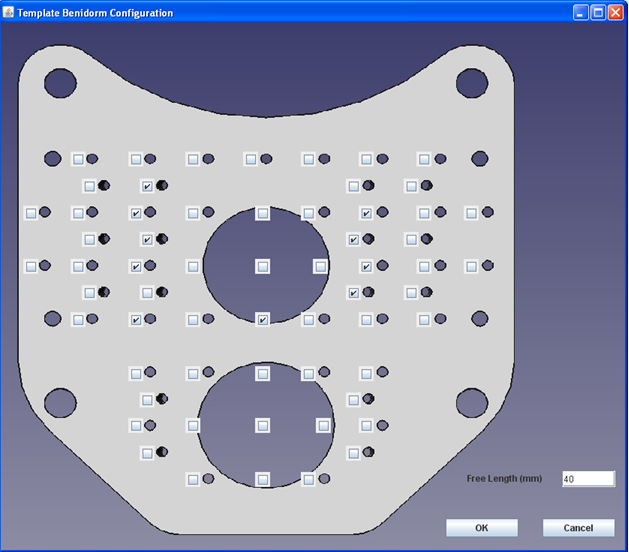
\includegraphics{img/Preplan1.png}

}

\caption{\label{fig-preplan1}Detalle de la aplicación desarrollada para
la configuración del TB}

\end{figure}

\begin{figure}

{\centering 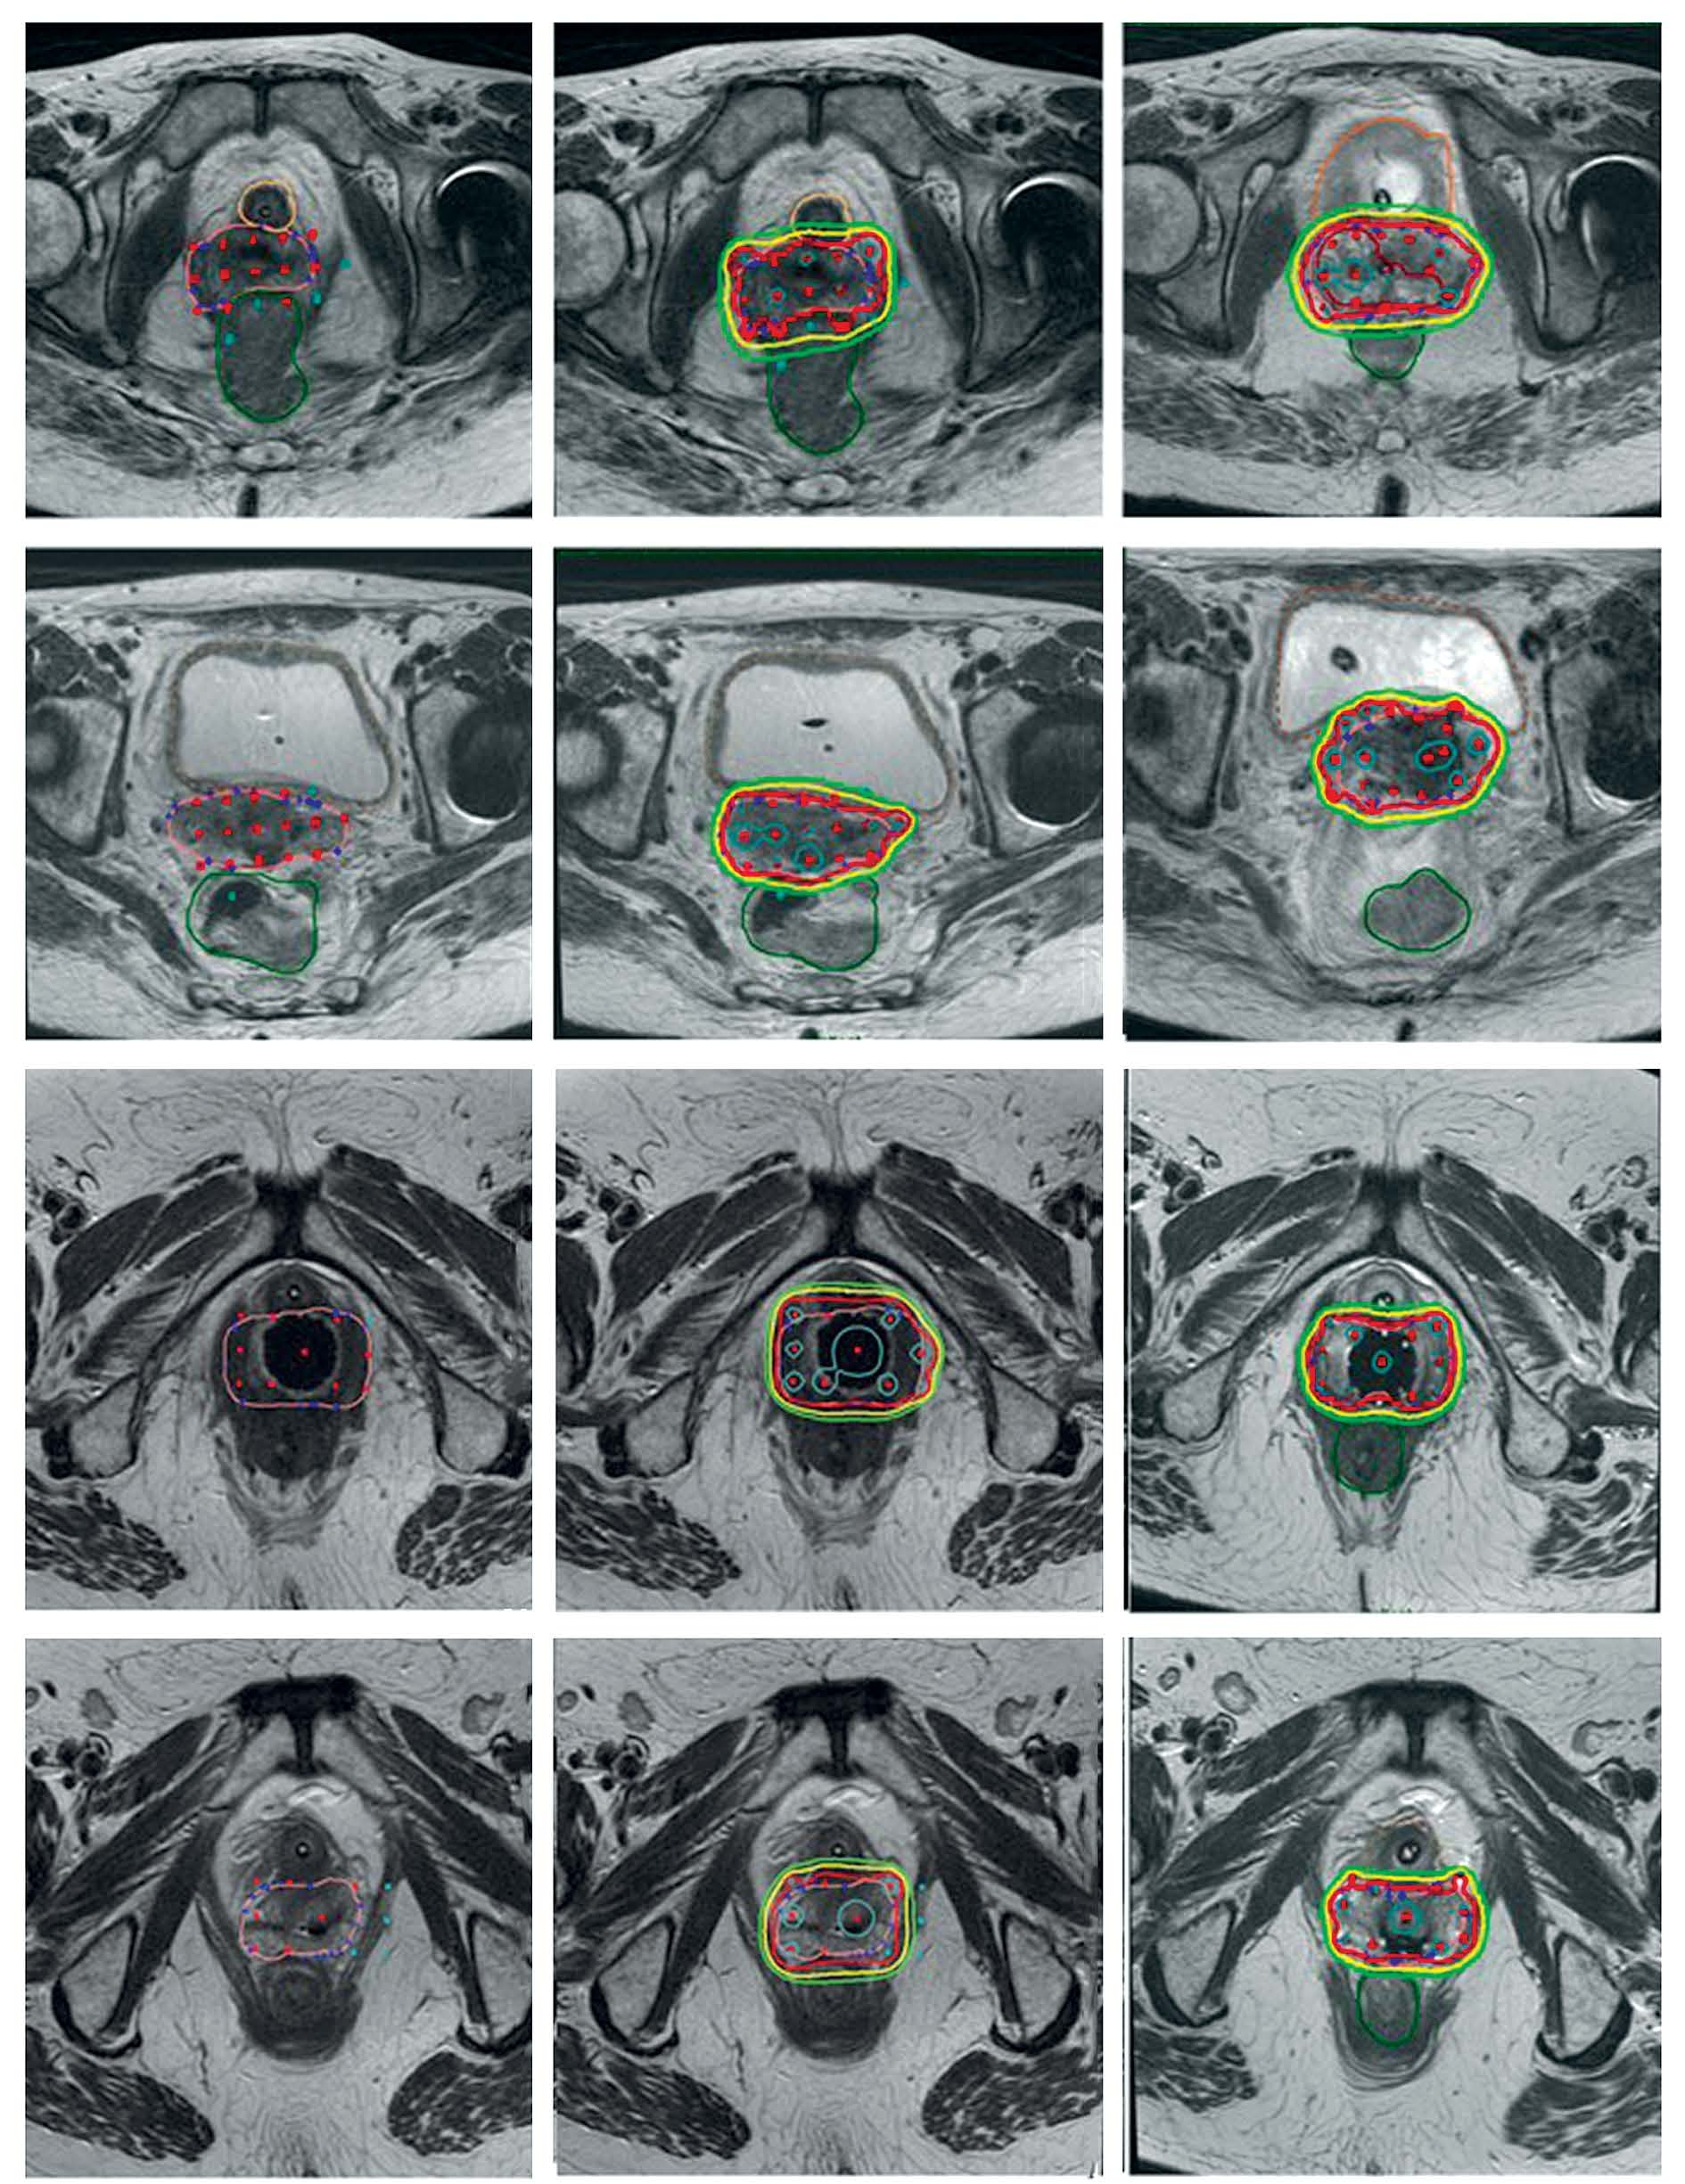
\includegraphics[width=6.25in,height=\textheight]{img/Preplan2.jpg}

}

\caption{\label{fig-preplan2}Filas 1 y 2 plan virtual antes del
implante. Filas 3 y 4 el implante final}

\end{figure}

\hypertarget{review-on-treatment-planning-systems-for-cervix-brachytherapy-interventional-radiotherapy-some-desirable-and-convenient-practical-aspects-to-be-implemented-from-radiation-oncologist-and-medical-physics-perspectives-otal2022-publicado-en-julio-2022-1}{%
\section{Review on Treatment Planning Systems for Cervix Brachytherapy
(Interventional Radiotherapy): Some Desirable and Convenient Practical
Aspects to Be Implemented from Radiation Oncologist and Medical Physics
Perspectives (Otal2022 publicado en julio
2022)}\label{review-on-treatment-planning-systems-for-cervix-brachytherapy-interventional-radiotherapy-some-desirable-and-convenient-practical-aspects-to-be-implemented-from-radiation-oncologist-and-medical-physics-perspectives-otal2022-publicado-en-julio-2022-1}}

Después de que los especialistas presentaran las demostraciones,
respondieron las preguntas planteadas por los autores. Sus respuestas al
cuestionario se resumen en esta sección siguiendo el esquema descrito en
la sección Materiales y Métodos, junto con los comentarios de los
autores.

\hypertarget{sec-a1}{%
\subsection{A1---Herramientas de puesta en marcha y control de
calidad}\label{sec-a1}}

Sólo uno de los TPS permite la modificación de la ruta de origen dentro
de la biblioteca de aplicadores. Es fundamental para aplicadores curvos,
como anillos u ovoides, donde la fuente suele moverse cerca de la pared
del aplicador y lejos del eje de simetría.

De los tres TPSs analizados, sólo dos incluyen la posibilidad de
realizar cálculos de MBDCA. Ninguno de los casos de prueba disponibles
en eal momento en que se escribió el manuscrito eran casos clínicos
ginecológicos aunque WG-DCAB actualmente está desarrollando casos de
prueba específicos para ginecología. Sin embargo, el Caso de Prueba 4,
aunque no se parece del todo a una situación clínica, incorpora un
aplicador ginecológico genérico blindado y, por tanto, es la más
interesante para que el usuario clínico ponga en marcha el TPS. Ninguno
de los TPSs analizados incorpora un conjunto completo de herramientas
para realizar este proceso de puesta en marcha, lo que requiere que el
usuario clínico utilice herramientas externas, como
BrachyGuide\textsuperscript{\protect\hyperlink{ref-pantelis2015}{101}} o
AMIGO\textsuperscript{\protect\hyperlink{ref-fonseca2014}{102}}.

En cuanto a la puesta en marcha del cálculo de dosis por parte del TG43,
los autores creen que el procedimiento de verificación no es todo lo
operativo que debería. La dosis que devuelve el TPS para puntos
específicos se comparará con las tablas de consenso utilizando las
funciones del protocolo TG43 para un modelo fuente determinado. Sin
embargo, estos puntos sólo se pueden ingresar mediante el teclado y uno
a uno. Es deseable un método más ágil y menos propenso a errores.

\hypertarget{sec-a2}{%
\subsection{A2---Registro de imágenes y utilidades para gestionar
información de tratamientos previos}\label{sec-a2}}

Los tres TPS permiten un registro rígido, aunque solamente uno incluye
la posibilidad de registro de imagen deformable.

En teoría, el registro deformable coincidiría y sumaría cada dosis de
vóxel combinando cada fracción de EBRT con la contribución
correspondiente de BT. Sin embargo, ninguno de los TPS disponibles
incluye la tecnología necesaria para rastrear el efecto en estructuras
biológicamente significativas dentro de los volúmenes objetivo y OAR sin
utilizar software externo compatible. Por esta razón, GEC-ESTRO
recomienda asumir que las paredes de los órganos adyacentes al aplicador
de BT y los volúmenes objetivo recibieron la dosis prescrita de EBRT.
Este enfoque conservador, que ya se utiliza ampliamente en la práctica
clínica, ha proporcionado resultados fiables tanto para los volúmenes
objetivo como para los OAR estáticos, a pesar de ser una suposición
bastante importante. Además, siguiendo una de las recomendaciones de
EMBRACE II para la planificación de EBRT, se podría generar una región
de control alrededor del CTV-HR de 10 mm de espesor para establecer un
requisito de homogeneidad de dosis con el fin de evitar puntos críticos
en los OAR cercanos al CTV-HR, que probablemente también recibirán una
dosis considerable de BT. Se debe prestar especial atención en los casos
de EBRT con múltiples PTVs y dosis debido a las dosis más altas en los
D2cc de los OAR.

\hypertarget{sec-a3}{%
\subsection{A3---Contorneo en MRI. Eliminar la componente
intracavitaria}\label{sec-a3}}

Ninguno de los TPSs permite retirar el anillo u los ovoides de la MRI.
En el caso de utilizar bibliotecas de aplicadores para la
reconstrucción, la información sobre la posición del aplicador junto con
su composición podría ayudar a resolver este problema en futuras
versiones de los TPSs.

\hypertarget{sec-a4}{%
\subsection{A4---Reconstrucción de catéteres. Bibliotecas de la
componente intracavitaria}\label{sec-a4}}

Todos los TPS analizados tienen acceso a bibliotecas virtuales de
aplicadores intracavitarios para la reconstrucción de catéteres. Como se
discutió anteriormente, es útil para facilitar y reducir la
incertidumbre en la fase de reconstrucción. La DR es una alternativa a
este tipo de reconstrucción y la única solución para aplicadores no
rígidos, especialmente para la parte intersticial, disponible
comercialmente. Sin embargo, tomando el ejemplo de la reconstrucción de
un aplicador de anillo que incluye un tándem, ambas partes deben
tratarse como dos elementos diferentes de la biblioteca de aplicadores.
Por otra parte, el tándem está unido al anillo, por lo que no son
estrictamente independientes y pueden ofrecer restricciones geométricas
adicionales que podrían usarse para mejorar su reconstrucción. Sería
deseable desarrollar más esta idea.

Todos los especialistas mencionan la intención de mejorar el algoritmo
de colocación automática en los conjuntos de imágenes de resonancia
magnética porque reconocieron la incertidumbre inherente en todos los
casos. Los TPSs ya incorporan dichas herramientas, pero sólo son
precisas cuando se utilizan en imágenes de CT. Hrinivich et
al.\textsuperscript{\protect\hyperlink{ref-hrinivich2019}{103}} han
desarrollado un método de auto-reconstrucción del anillo y del tándem
utilizando imágenes de resonancia magnética ponderadas en T2 con un
algoritmo basado en el registro del modelo de superficie tridimensional,
optimizado maximizando el gradiente de intensidad de la imagen normal a
la superficie del modelo.

\hypertarget{sec-a5}{%
\subsection{A5---Reconstrucción de agujas. Parte
intersticial}\label{sec-a5}}

En el caso de la reconstrucción de la parte intersticial, los TPS
permiten reconstruir las agujas a través de la zona negra que dejan las
agujas de plástico y el desplazamiento entre la punta y la primera
posición de parada. Sin embargo, en algunos casos el área negra no se ve
con suficiente claridad para realizar dicha reconstrucción de manera
eficiente.

En la misma línea, tal y como se ha comentado para la parte
intracavitaria, el recorrido de la aguja no es del todo independiente
del resto del aplicador. Richart et
al.\textsuperscript{\protect\hyperlink{ref-richart2015}{83}} sugieren un
método para reconstruir las agujas en el aplicador de Utrecht (Elekta,
Veenendaal, Países Bajos) basado en la longitud insertada de cada aguja
según lo informado por el oncólogo radioterápico en el momento de la
inserción. Esta distancia se determina utilizando una regla grabada en
la herramienta de inserción (ver figura~\ref{fig-utrecht_tool2}). En
otras palabras, la distancia entre el orificio de salida del aplicador y
la punta de la aguja es la distancia denominada \emph{free length}.

Tomando el concepto de \emph{free length}, Otal et
al.\textsuperscript{\protect\hyperlink{ref-otal2017}{80}} desarrollaron
un método para incluir el componente intersticial como un elemento de la
biblioteca de aplicadores. En tal modelo, las agujas salen de los
agujeros del ovoide. Tienen una longitud igual a la \emph{free length} y
a la dirección de la cavidad en el ovoide. Una vez colocada la primera
parte, se colocan las agujas sobre la zona negra, realizando rotaciones
alrededor del orificio de salida, manteniendo el punto de salida del
ovoide invariante.

Paralelamente a las soluciones basadas en bibliotecas de aplicadores,
algunos grupos continúan trabajando en métodos de reconstrucción
directa. Aunque el diámetro de la aguja es un desafío para el desarrollo
de \emph{dummies}, ya se están desarrollando posibles soluciones. Shaaer
et al.\textsuperscript{\protect\hyperlink{ref-shaaer2020}{104}} han
probado una \emph{dummy} para resonancia magnética destinada a la
componente intersticial. En una publicación posterior, con la ayuda de
esos marcadores, el mismo grupo realizó una segmentación automática del
catéter utilizando una red neuronal convolucional utilizando el modelo
U-Net, realizando una reconstrucción con aguja después de un post
procesado de la segmentación
previa\textsuperscript{\protect\hyperlink{ref-shaaer2021}{105}}.

\hypertarget{sec-a6}{%
\subsection{A6---Interpolación de imágenes}\label{sec-a6}}

Dos de los tres TPSs estudiados incluyen la probabilidad de acceder a
cortes interpolados entre dos adquiridos. El tercer TPS tiene modelos de
agujas en su biblioteca de aplicadores, pero sólo en el caso de las
rectas. Todos los especialistas mencionaron la intención del fabricante
de mejorar el algoritmo de colocación automática en los conjuntos de
imágenes de resonancia magnética porque reconocieron la importante
incertidumbre en las versiones actuales de los TPSs.

\hypertarget{sec-a7}{%
\subsection{A7---Uso del EQD2 en la optimización del
tratamiento}\label{sec-a7}}

Sólo uno de los TPSs tiene la opción de importar la información
dosimétrica de las fracciones dadas previamente. En este caso, la
información del DVH se agrega directamente a la planificación de BT y se
transforma a unidades EQD2 en función de los valores α/β introducidos
por el usuario. No hay una suma de las distribuciones de dosis y los DVH
solamente se extraen de las fracciones de EBRT. Sería más conveniente si
dicho proceso iterativo se integrara en el TPS y se incorporara a la
fase de optimización.

\hypertarget{sec-a8}{%
\subsection{A8---Uso del EQD2 para evaluar el tratamiento con la parte
de radioterapia externa. Restricciones óptimas y
obligatorias}\label{sec-a8}}

Para obtener el efecto biológico de las fases EBRT y BT en términos de
EQD2, es necesario sumar la contribución de las fracciones de BT dadas
con la mayor precisión
posible\textsuperscript{\protect\hyperlink{ref-kessler2006}{106}}. Si
bien todos los especialistas coincidieron en la importancia de este
punto, los TPSs actuales carecen de las herramientas necesarias para
optimizar las fracciones BT considerando las fracciones EBRT dadas
anteriormente.

Swamidas et
al.\textsuperscript{\protect\hyperlink{ref-swamidas2020}{93}} y Kim et
al.\textsuperscript{\protect\hyperlink{ref-kim2021}{107}} proporcionan
una descripción general del estado actual del registro de imágenes para
la acumulación de dosis en BT ginecológica guiada por imágenes, incluida
la combinación con radioterapia externa. Ambos estudios de revisión
concluyen que, aunque los algoritmos de registro de imágenes deformables
son una herramienta prometedora para la acumulación de dosis de EBRT, BT
y BT multi fraccionada, se requiere más investigación y desarrollo antes
de que estén listos para su aplicación clínica, especialmente para
evaluar las incertidumbres que surgen del registro deformable.

Los TPSs actuales tienen limitaciones al calcular distribuciones de
dosis acumuladas y al derivar un DVH compuesto de los planes EBRT y BT
en EQD2. Sería deseable promover la investigación y evolución de
algoritmos de registro deformable y adaptarlos a las complejidades de la
planificación del tratamiento de radioterapia de cérvix.

\hypertarget{sec-a9}{%
\subsection{A9---Bloqueo de pesos}\label{sec-a9}}

Todos los TPSs incluyen herramientas para modificar los tiempos de
permanencia: variación manual de tiempos, normalización a puntos o
líneas de referencia, renormalización general y optimización gráfica,
entre otras. La capacidad de bloquear catéteres individuales y
posiciones de permanencia, haciendo que los tiempos de permanencia no
sean modificables, solo se incluyó en uno de los TPSs. Esta herramienta
es de gran ayuda ya que facilita el control del peso de cada componente
(tándem, ovoides/anillo e intersticial).

\hypertarget{sec-a10}{%
\subsection{A10---Métodos de optimización. Registro de los parámetros
D90 y D2cc}\label{sec-a10}}

En todos los TPSs se ofrece optimización inversa basada en las métricas
dosimétricas objetivas (D90 , D2cc , \ldots). También se informa el
valor de D2cc extraído del DVH. Aunque estos módulos de optimización
tienen el potencial de ofrecer distribuciones de dosis clínicamente
aceptables, ninguno de los TPS proporcionó el control requerido del
gradiente de dosis alrededor de las agujas a pesar de tener parámetros
específicos para modularlo. Otra herramienta interesante ya incorporada
en los algoritmos de optimización inversa de EBRT es la posibilidad de
partir de una solución dada por el usuario y utilizarla como estado
inicial en el proceso de optimización. Los TPSs de BT serían mucho más
utiles si incorporasen la citada posibilidad.

\hypertarget{sec-a11}{%
\subsection{A11---Resolución de los histogramas
dosis-volumen}\label{sec-a11}}

Solamente uno de los TPSs analizados gestiona adecuadamente esta
cuestión. En los demás casos no se especificó claramente.

\hypertarget{sec-a12}{%
\subsection{A12---Localización de los puntos D2cc}\label{sec-a12}}

Todos los especialistas coincidieron en que la ubicación del parámetro
D2cc de cada uno de los OAR es fundamental. Uno de los TPSs incluye una
opción que localiza el plano con el valor máximo para una estructura
particular, mostrando la contribución de cada fuente a ese punto. El
resto no menciona ninguna solución similar.

Un valor numérico de D2cc como restricción en el recto y la vejiga no es
suficiente para predecir toxicidades posteriores. También es fundamental
conocer la posición en ese órgano. La ubicación particular de estos
puntos de dosis altas puede requerir una nueva optimización de la
distribución de dosis. Por lo tanto, los autores sostienen que es
crucial incluir en los TPS herramientas que hagan visibles estas áreas
de dosis altas o, incluso preferiblemente, incluir estas posiciones como
datos de entrada en futuros algoritmos de optimización.

\hypertarget{sec-a13}{%
\subsection{A13---Algoritmos de cálculo por heterogeneidad en BT
(MBDCA)}\label{sec-a13}}

Debido a su relevancia clínica, los tratamientos de cérvix estuvieron
entre los primeros en ser analizados desde la perspectiva de los MBDCA.
Se han realizado evaluaciones retrospectivas del impacto de las
heterogeneidades en el caso de los planes hechos con el sistema de
Manchester\textsuperscript{\protect\hyperlink{ref-mikell2012}{108}--\protect\hyperlink{ref-sinnatamby2016}{110}}.
Se informó de un pequeño impacto en los parámetros dosimétricos
calculados del TG-43, observándose cambios menores en las dosis de los
Puntos A y B y los parámetros volumétricos D2cc y D90. Se observaron
puntos calientes y fríos con una diferencia de aproximadamente el 10 \%
en ubicaciones particulares dentro del de los volúmenes así como que la
atenuación en las paredes del aplicador de titanio contribuyeron
aproximadamente en un 1,3 \% a estas reducciones. Hofbauer et
al.\textsuperscript{\protect\hyperlink{ref-hofbauer2016}{111}}
reevaluaron los planes de tratamiento administrados con aplicadores de
plástico en tándem y de anillo con componente intersticial con de 3 a 10
agujas adicionales cuando fue necesario. Los autores informaron de un
impacto dosimétrico mínimo, con D90 y V100 para CTV de alto riesgo
reducidos en menos del 0,5 \% y D2cc y D0,1cc para órganos de riesgo
reducidos en menos del 2 \%. Abe et
al.\textsuperscript{\protect\hyperlink{ref-abe2018}{112}} evaluaron el
impacto en el D2cc de recto de su contenido de gas en pacientes tratados
mediante diferentes técnicas. Los autores informaron diferencias con
respecto al TG-43 en el rango de 11,9 ± 2,6 \% (contenido total de gas)
a 0,8 ± 2,0 \% (lleno con material equivalente a agua).

Por lo tanto, está claro que, aunque los MBDCA pueden ofrecer
información adicional sobre las dosis depositadas, el impacto clínico de
las diferencias encontradas con respecto a los parámetros clínicos
basados en TG-43 son insignificantes para la BT de cérvix basada en
resonancia magnética.

\bookmarksetup{startatroot}

\hypertarget{artuxedculos}{%
\chapter{Artículos}\label{artuxedculos}}

\newpage{}

\hypertarget{a-method-to-incorporate-interstitial-components-into-the-tps-gynecologic-rigid-applicator-library.}{%
\section{A method to incorporate interstitial components into the TPS
gynecologic rigid applicator
library.}\label{a-method-to-incorporate-interstitial-components-into-the-tps-gynecologic-rigid-applicator-library.}}

\newpage{}

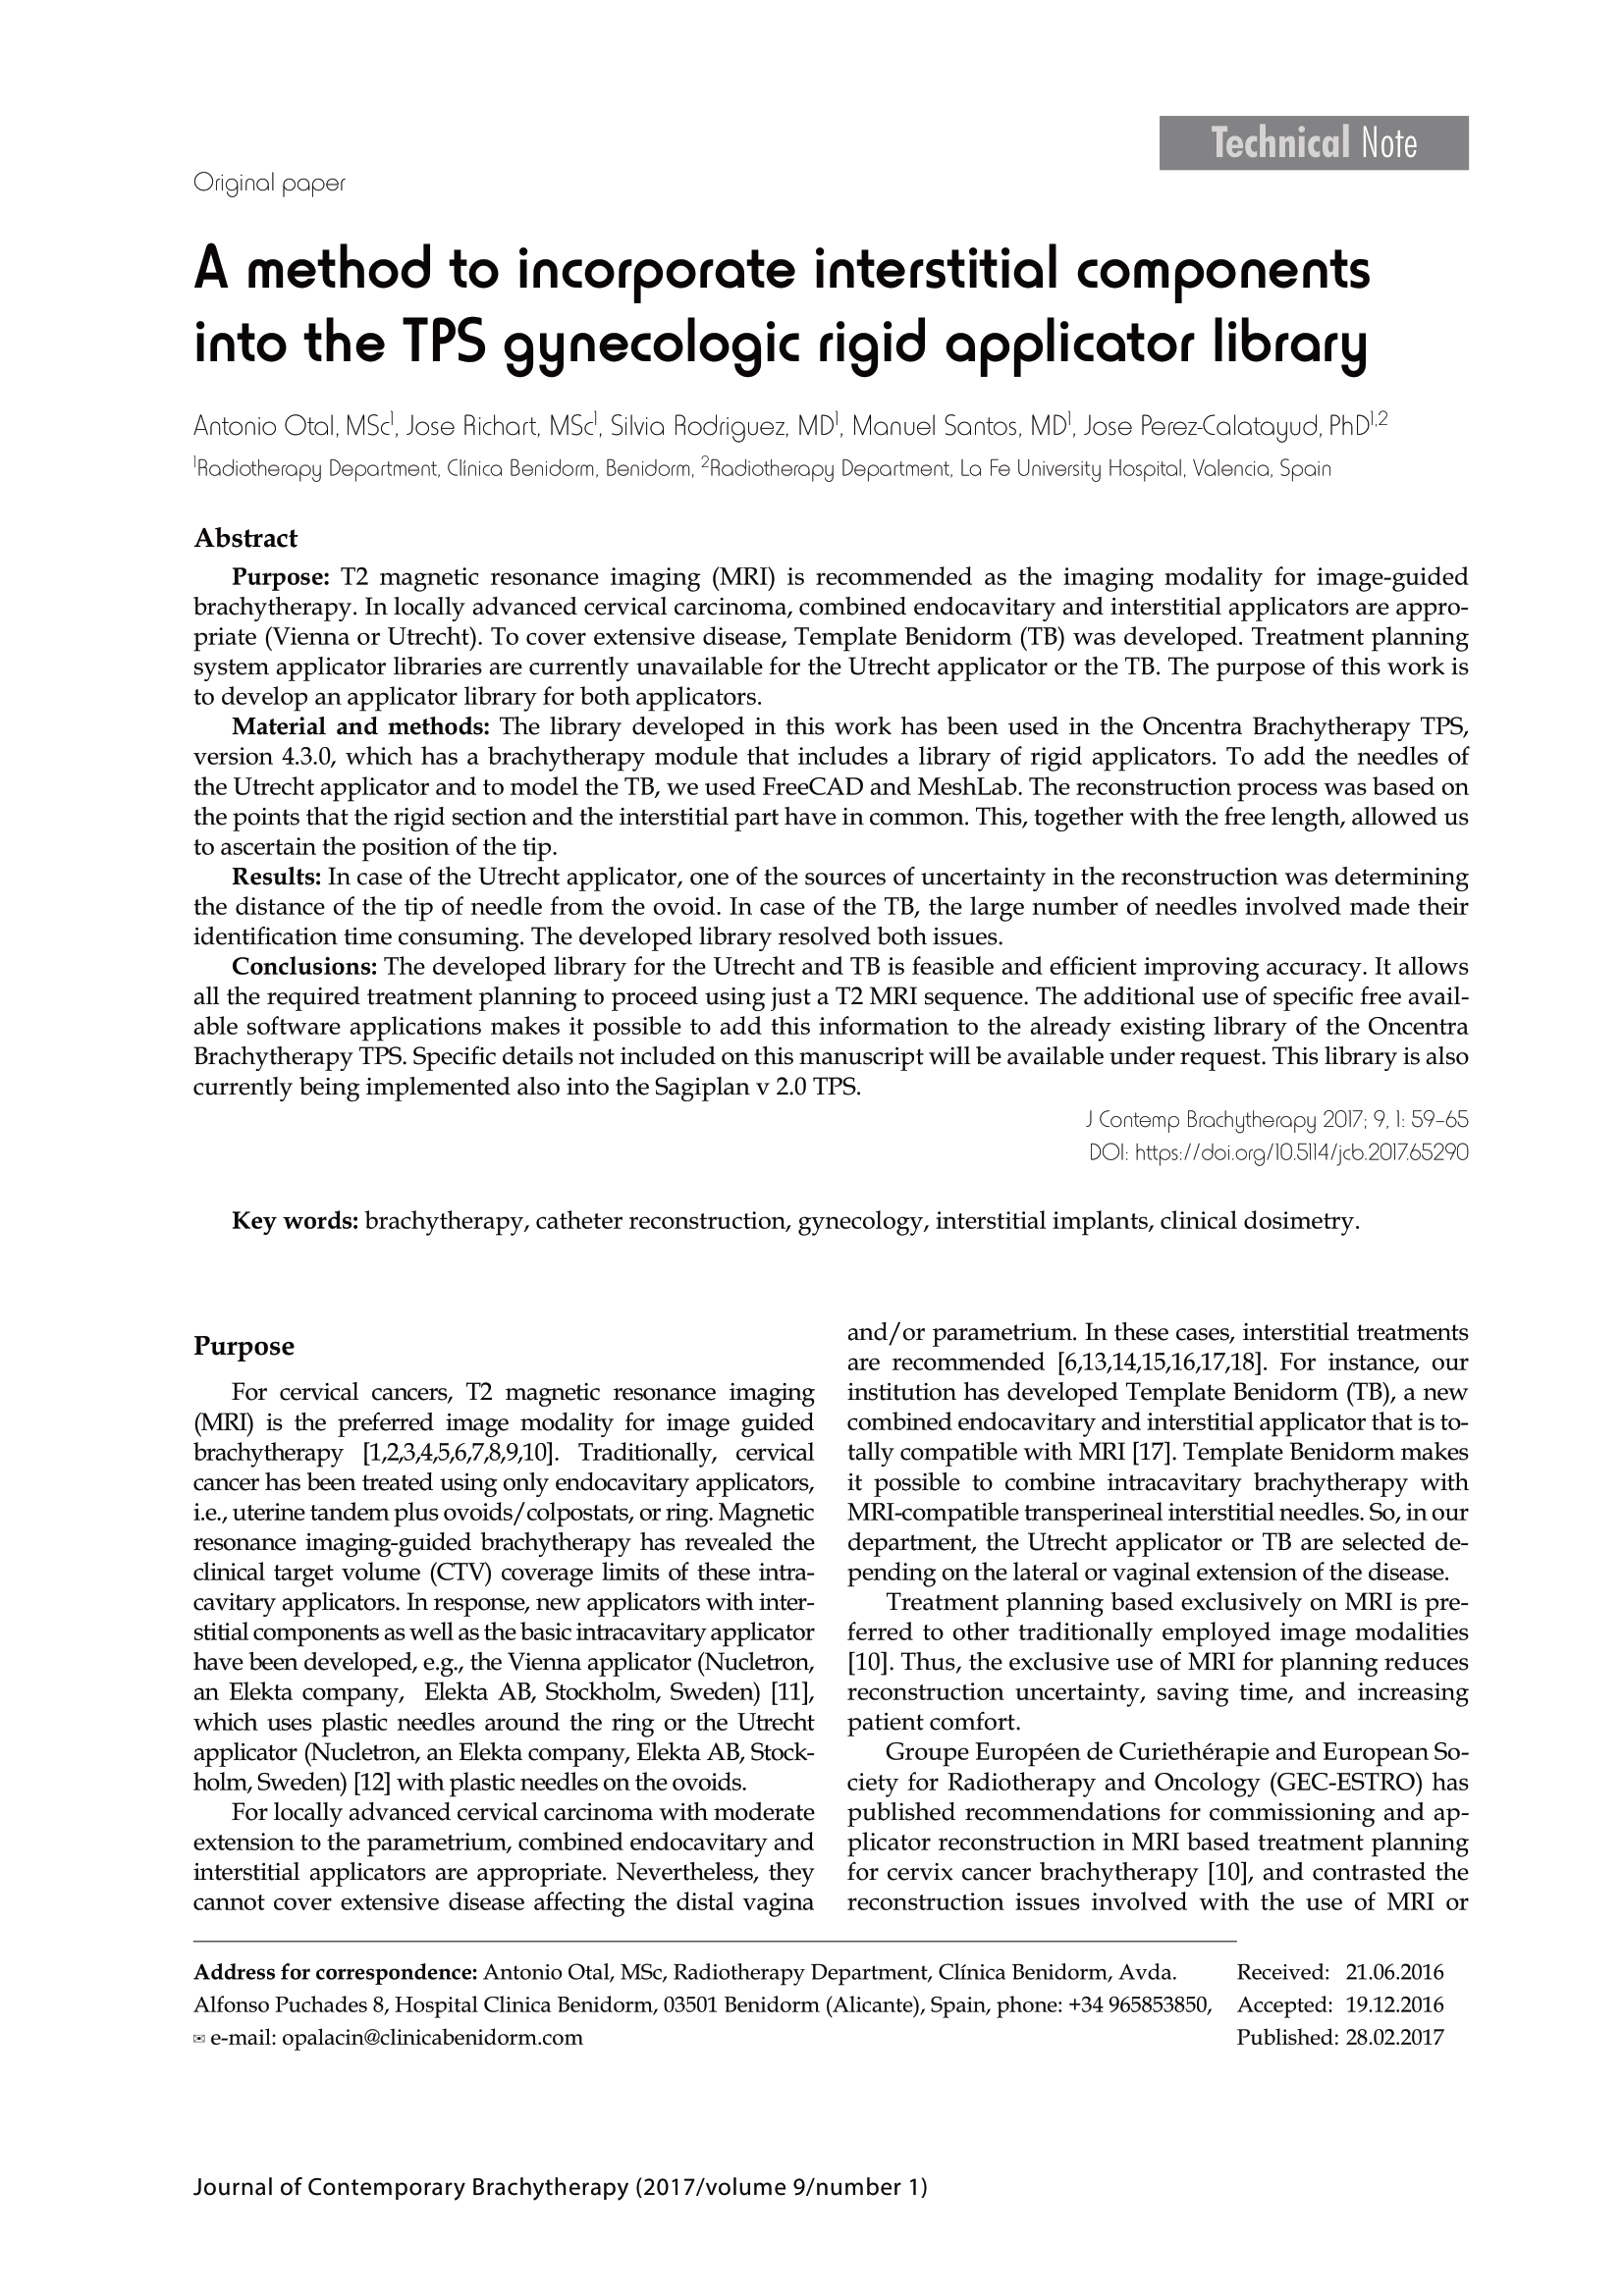
\includegraphics{articulos/librerias/librerias-1.png}
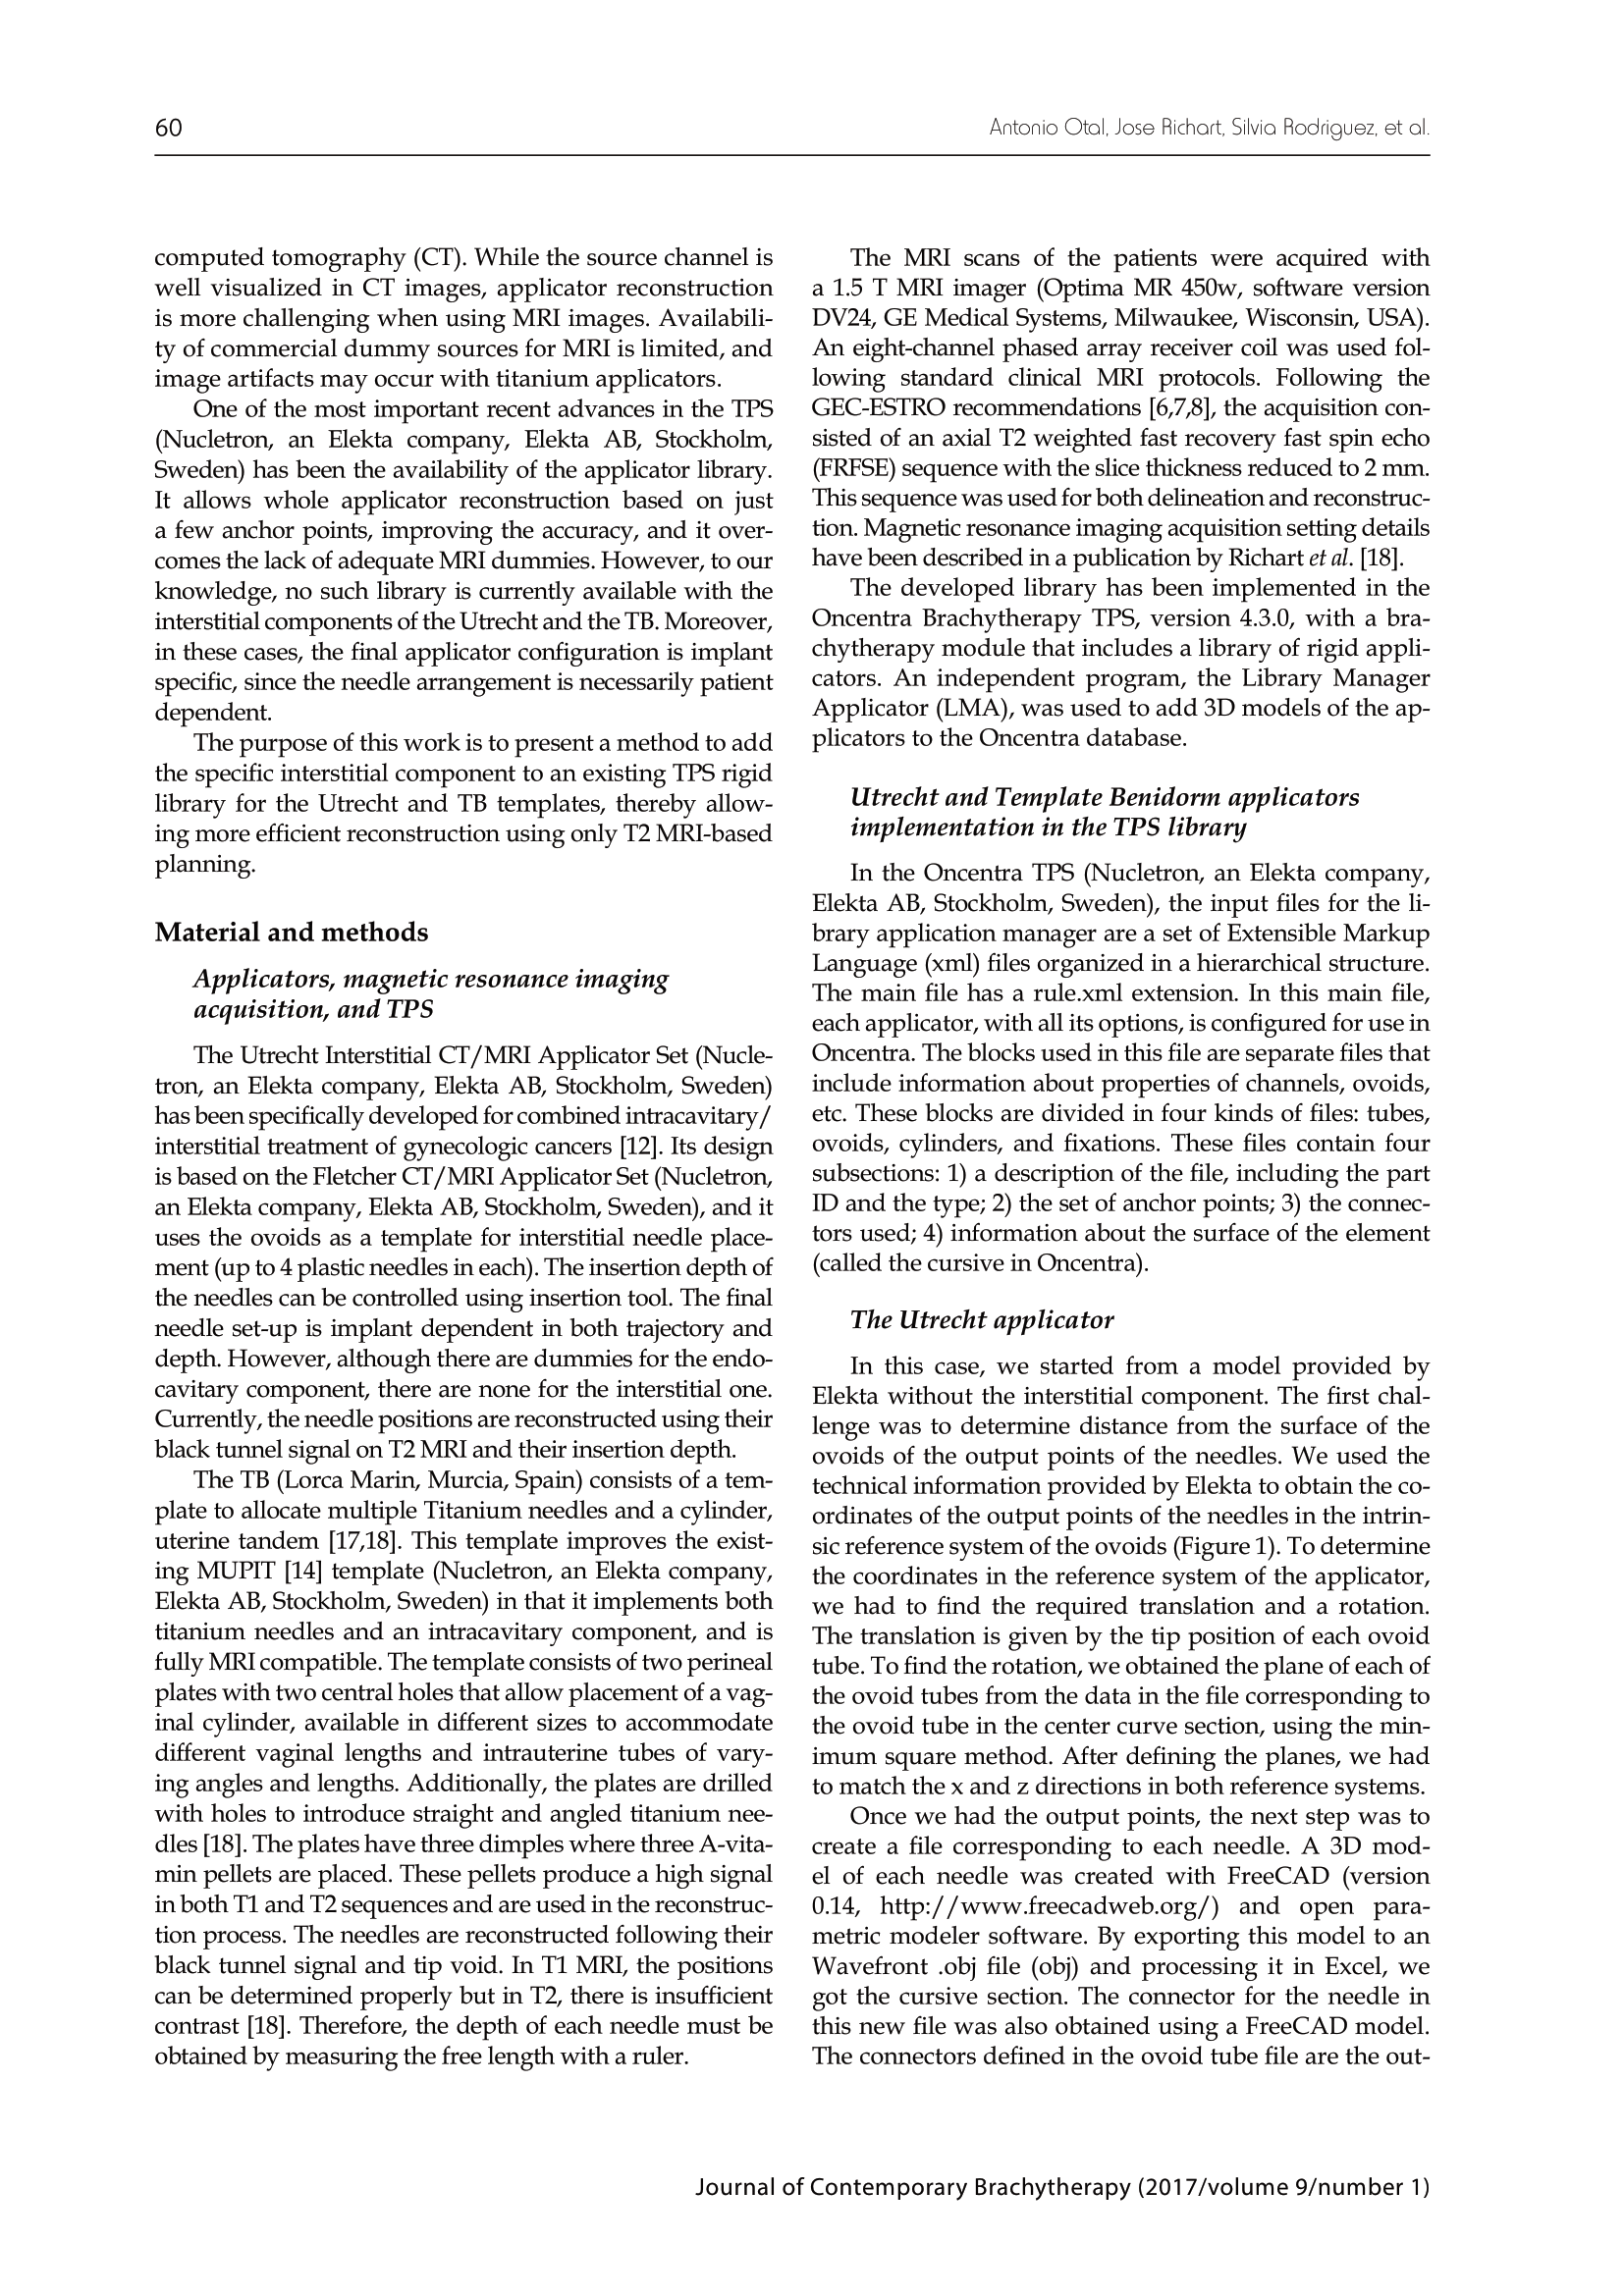
\includegraphics{articulos/librerias/librerias-2.png}
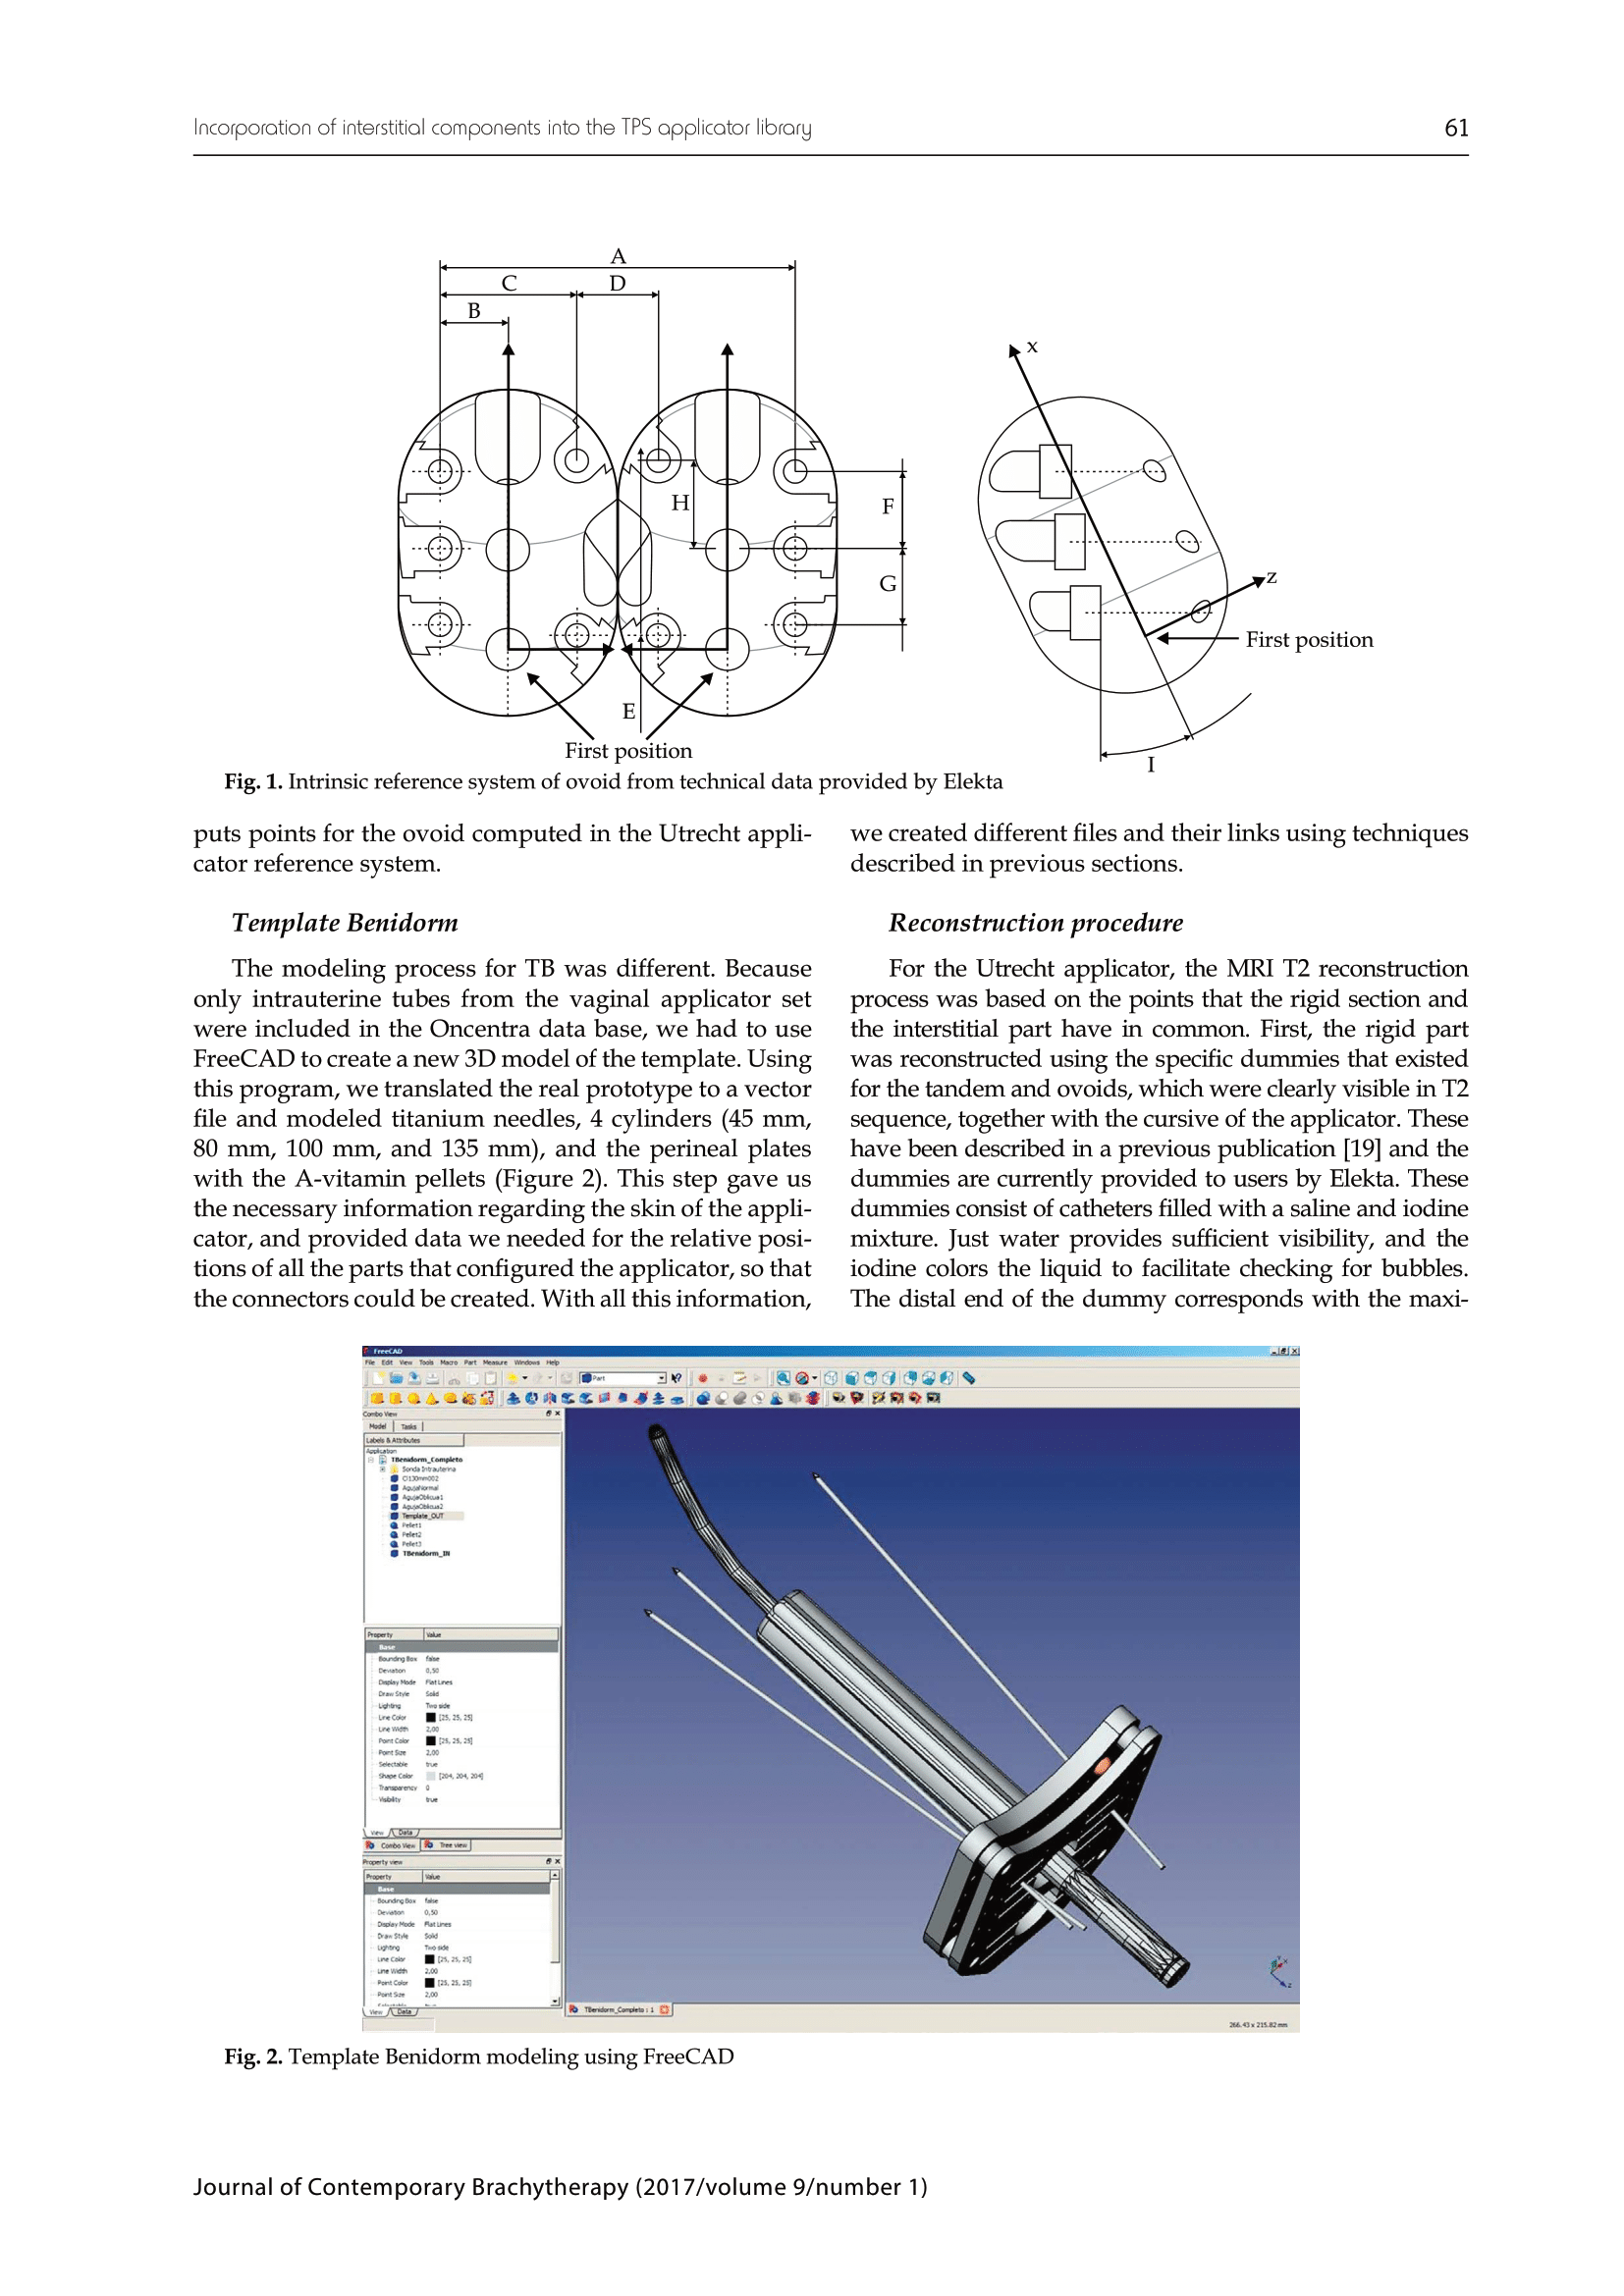
\includegraphics{articulos/librerias/librerias-3.png}
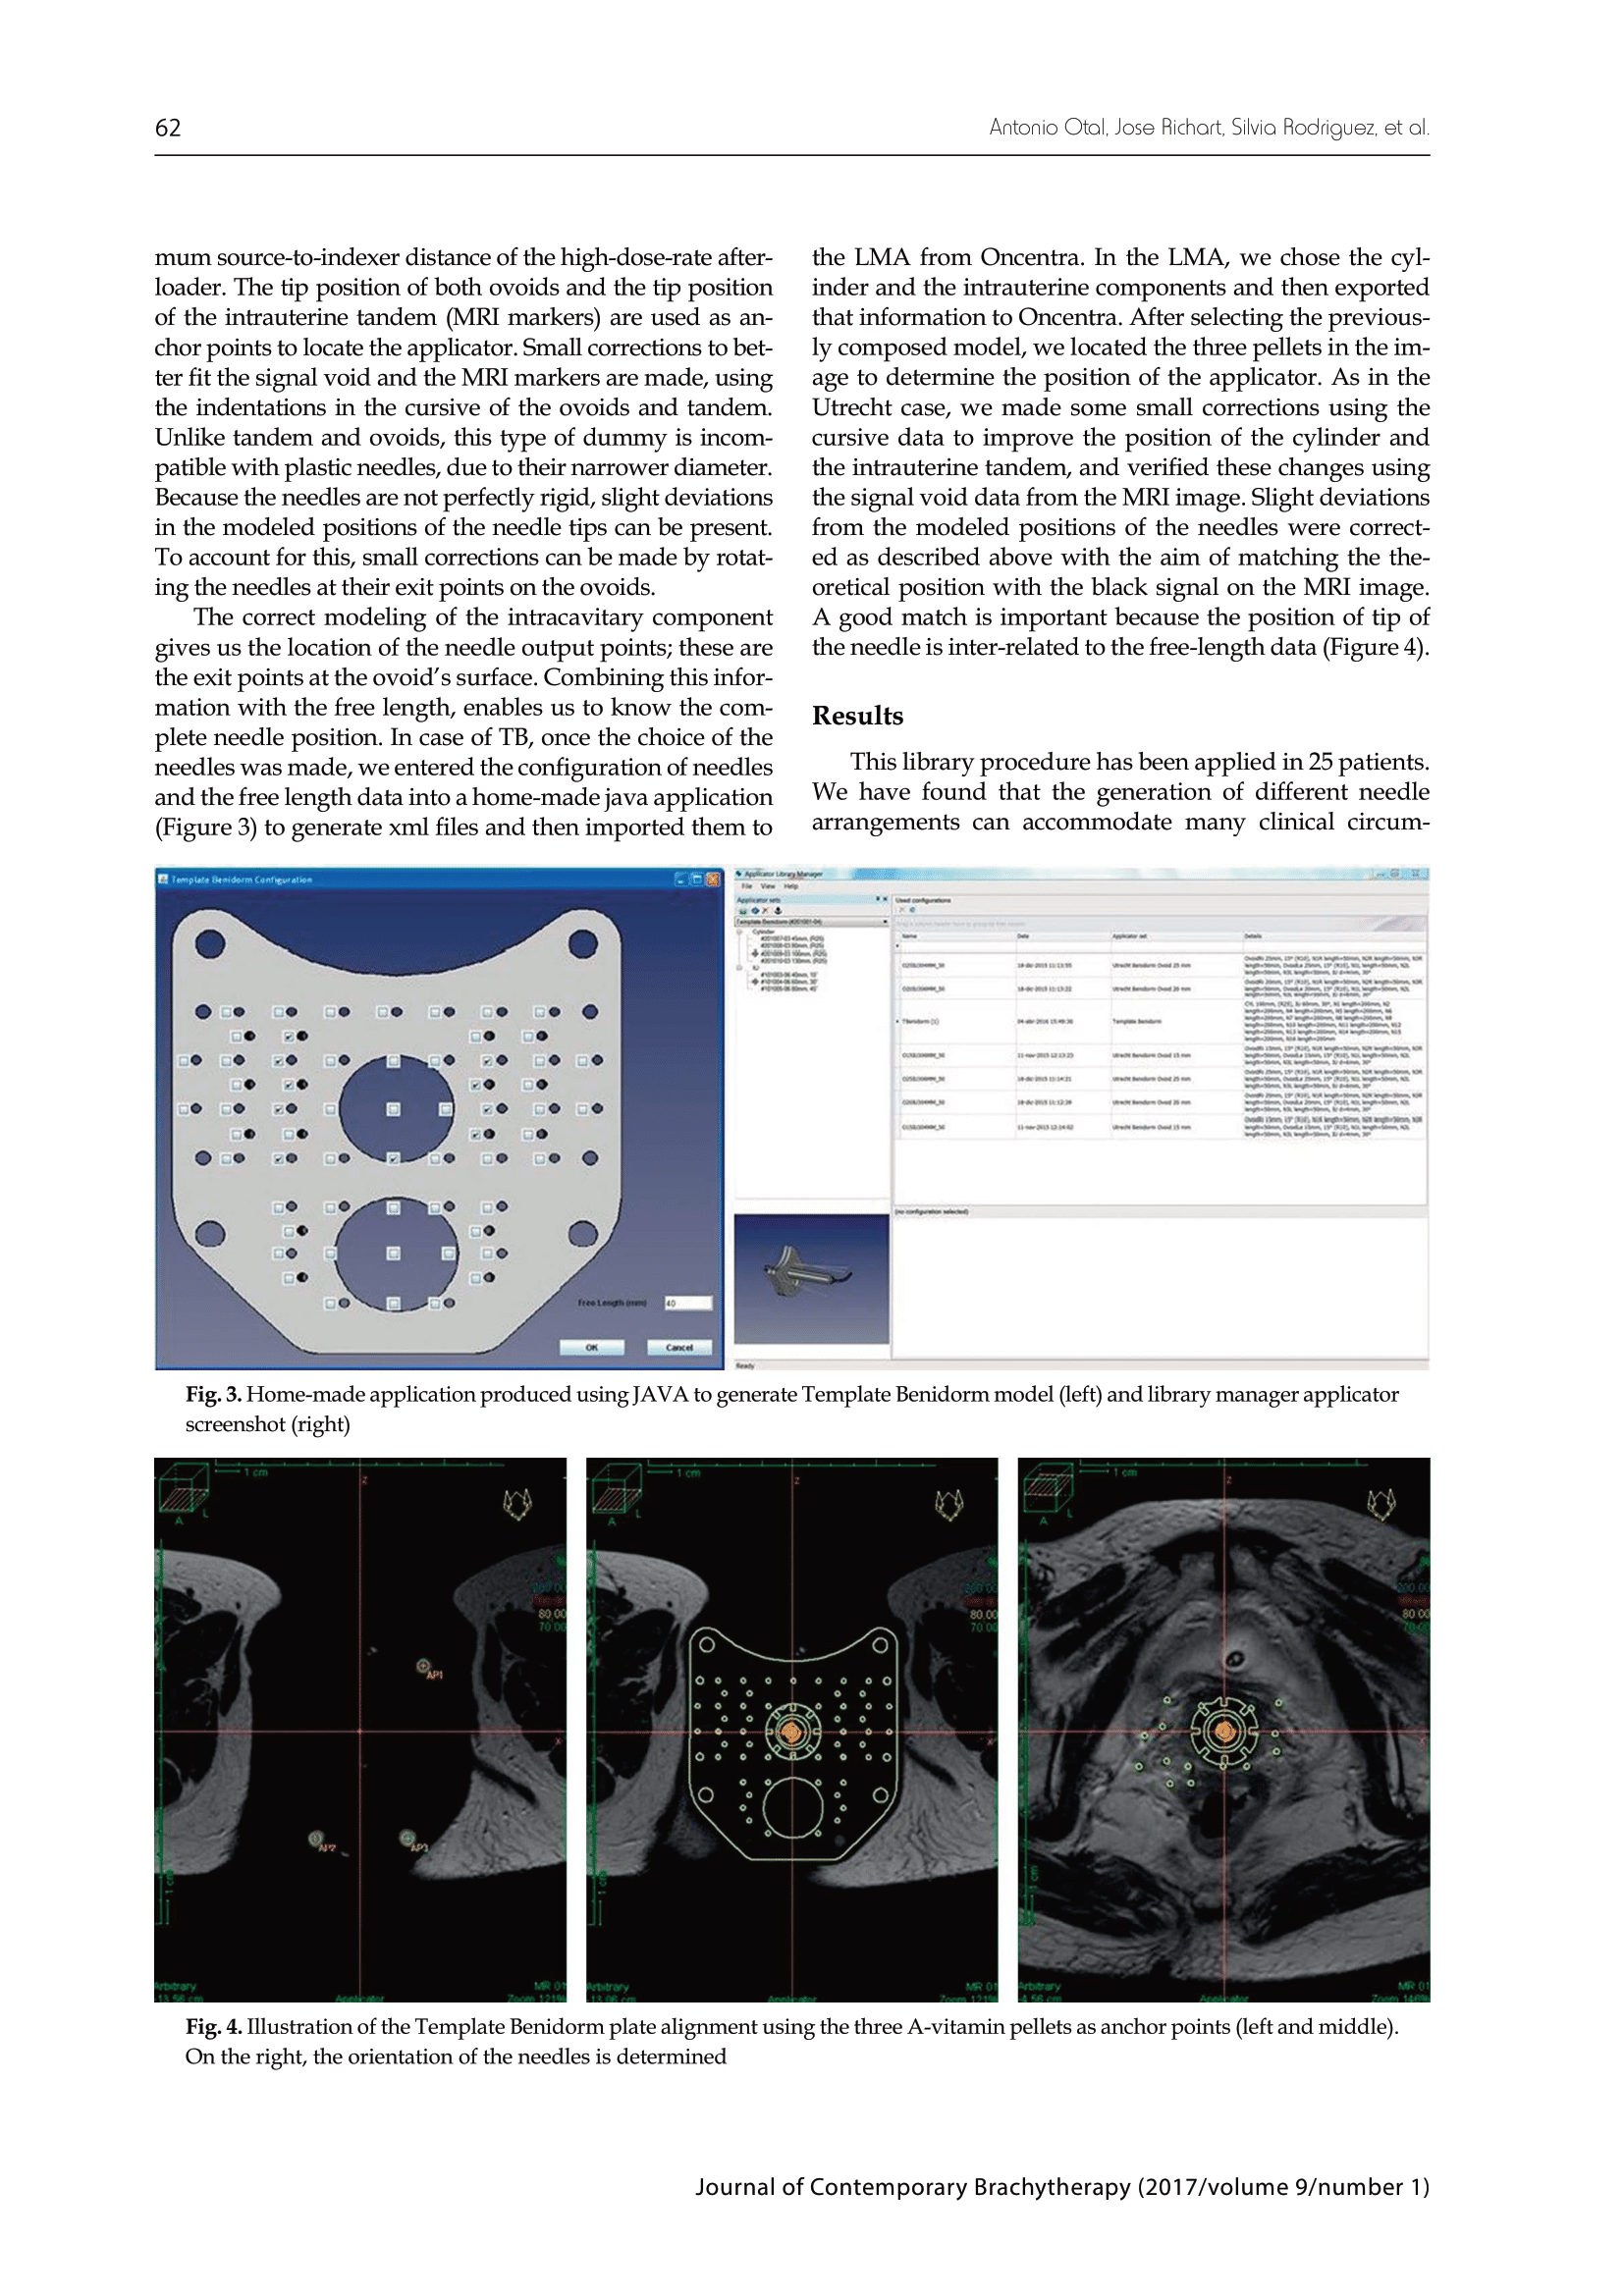
\includegraphics{articulos/librerias/librerias-4.png}
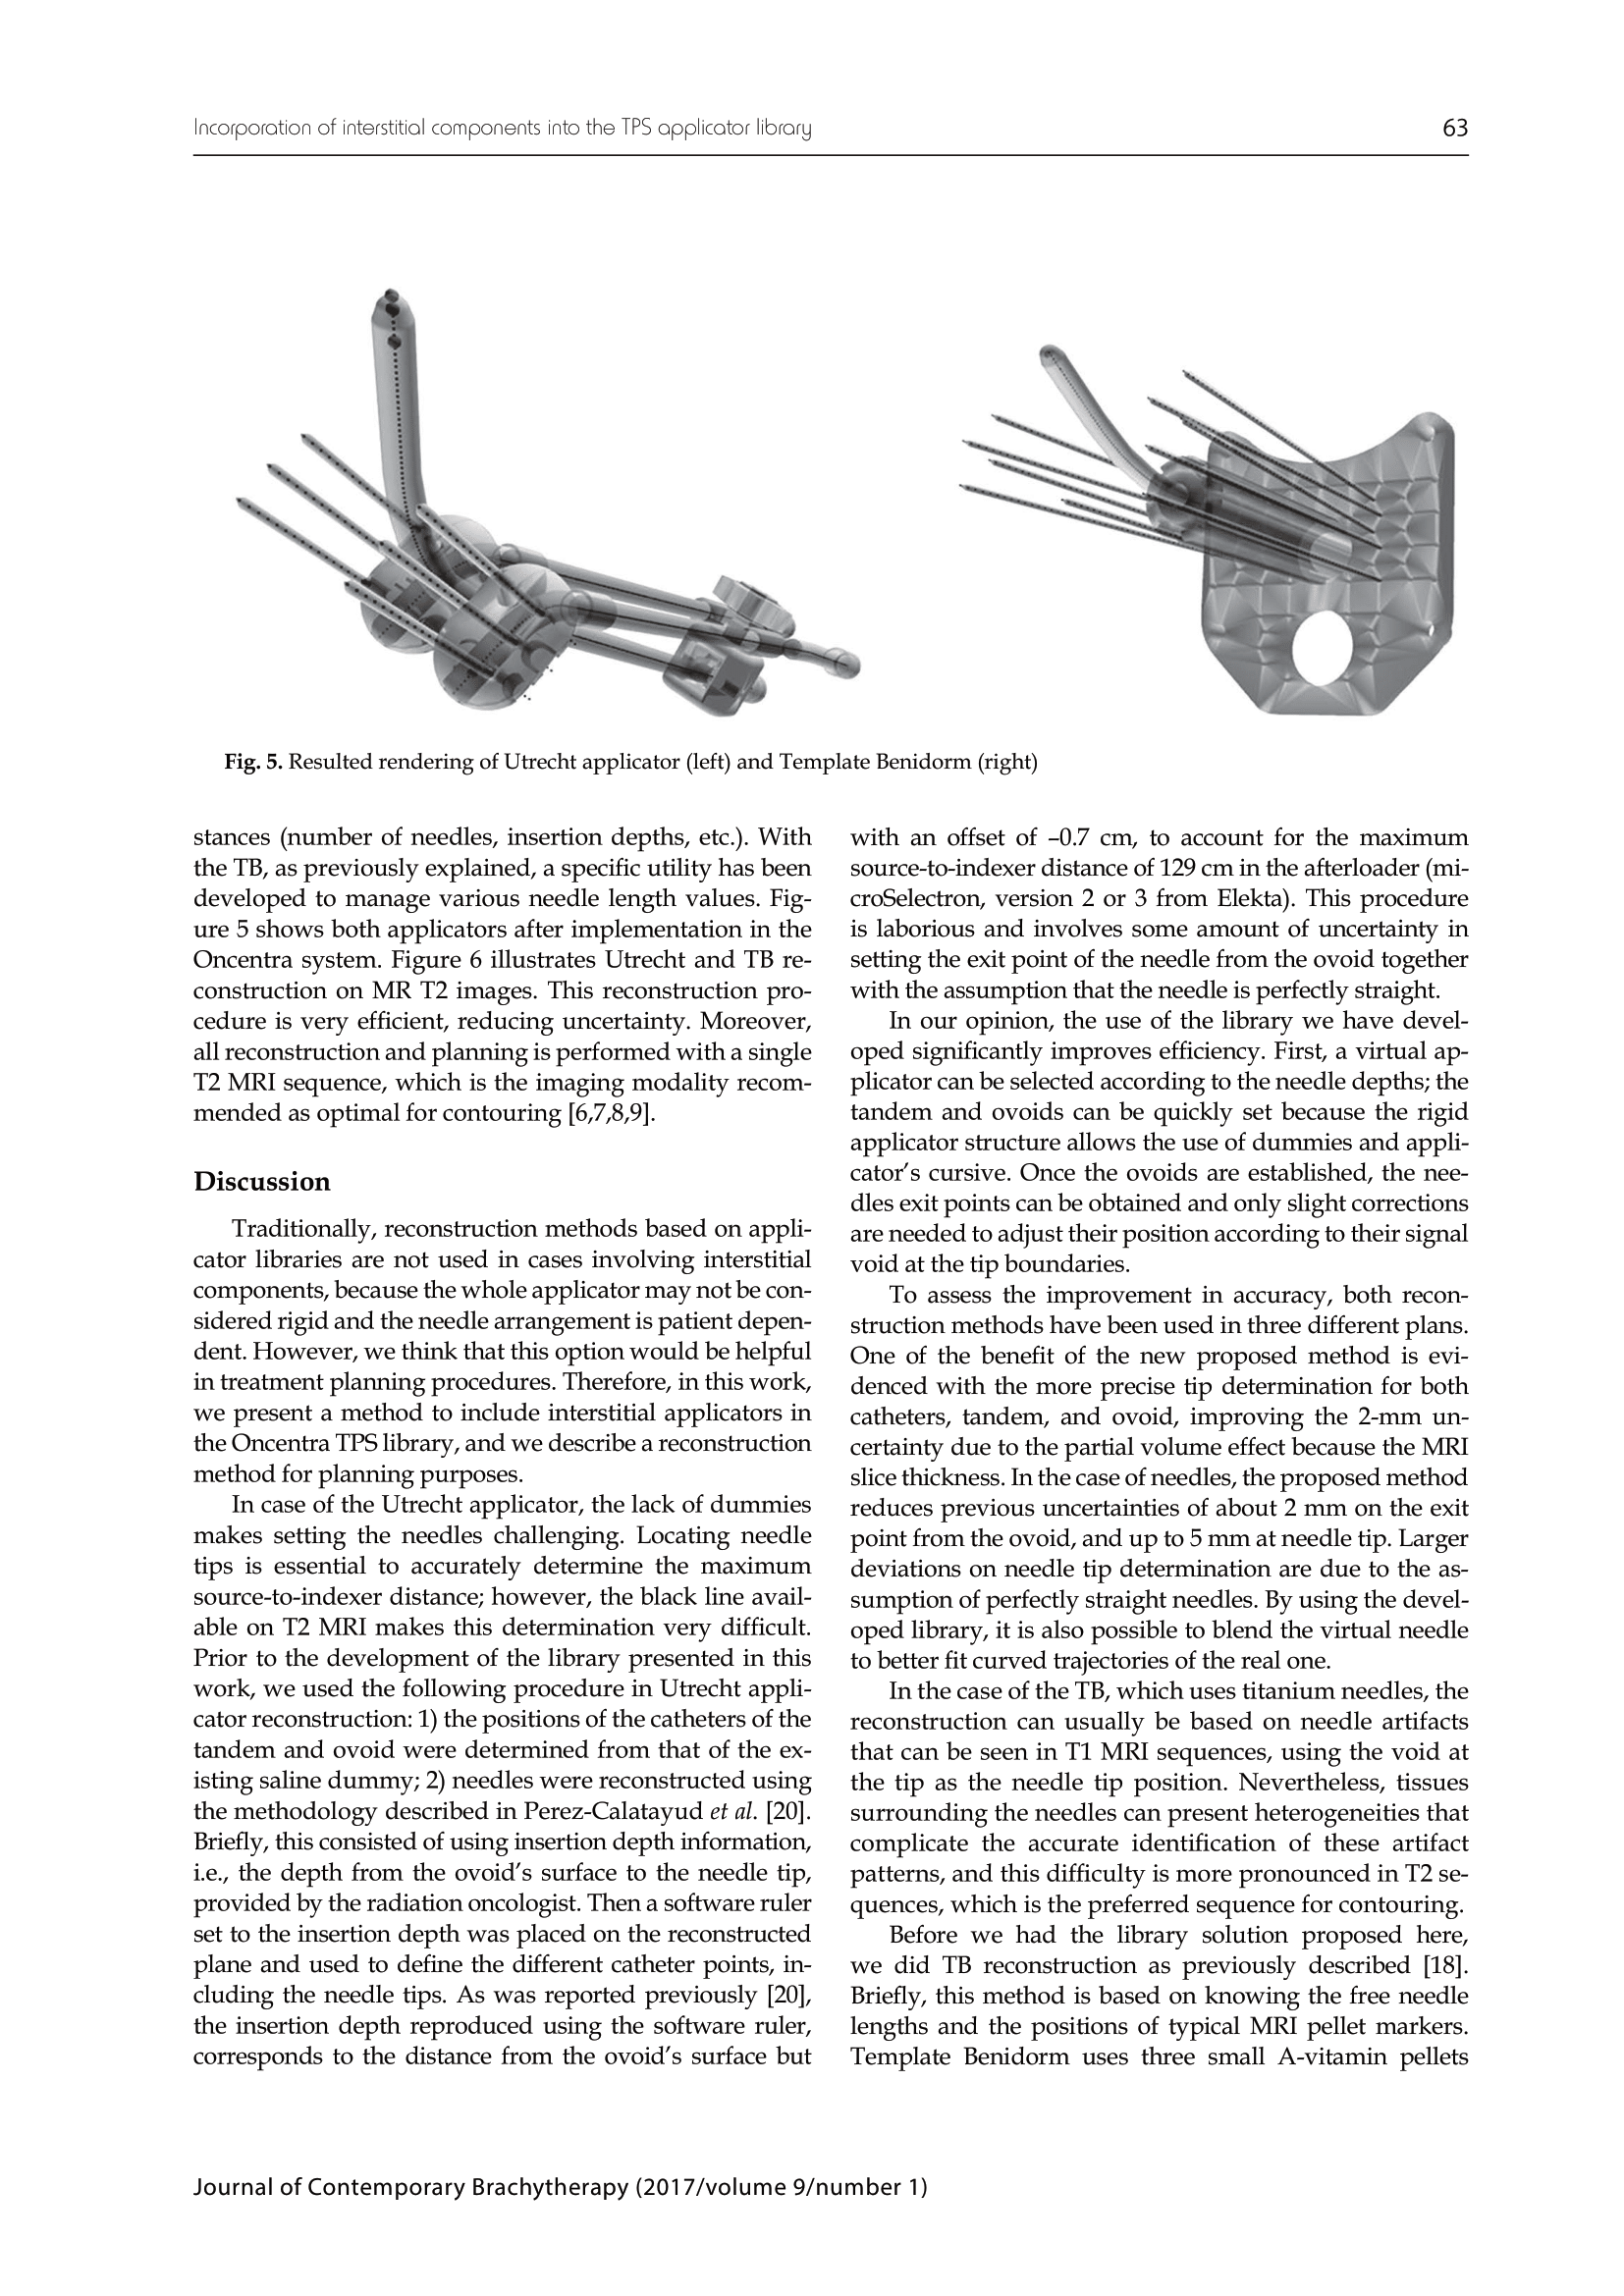
\includegraphics{articulos/librerias/librerias-5.png}
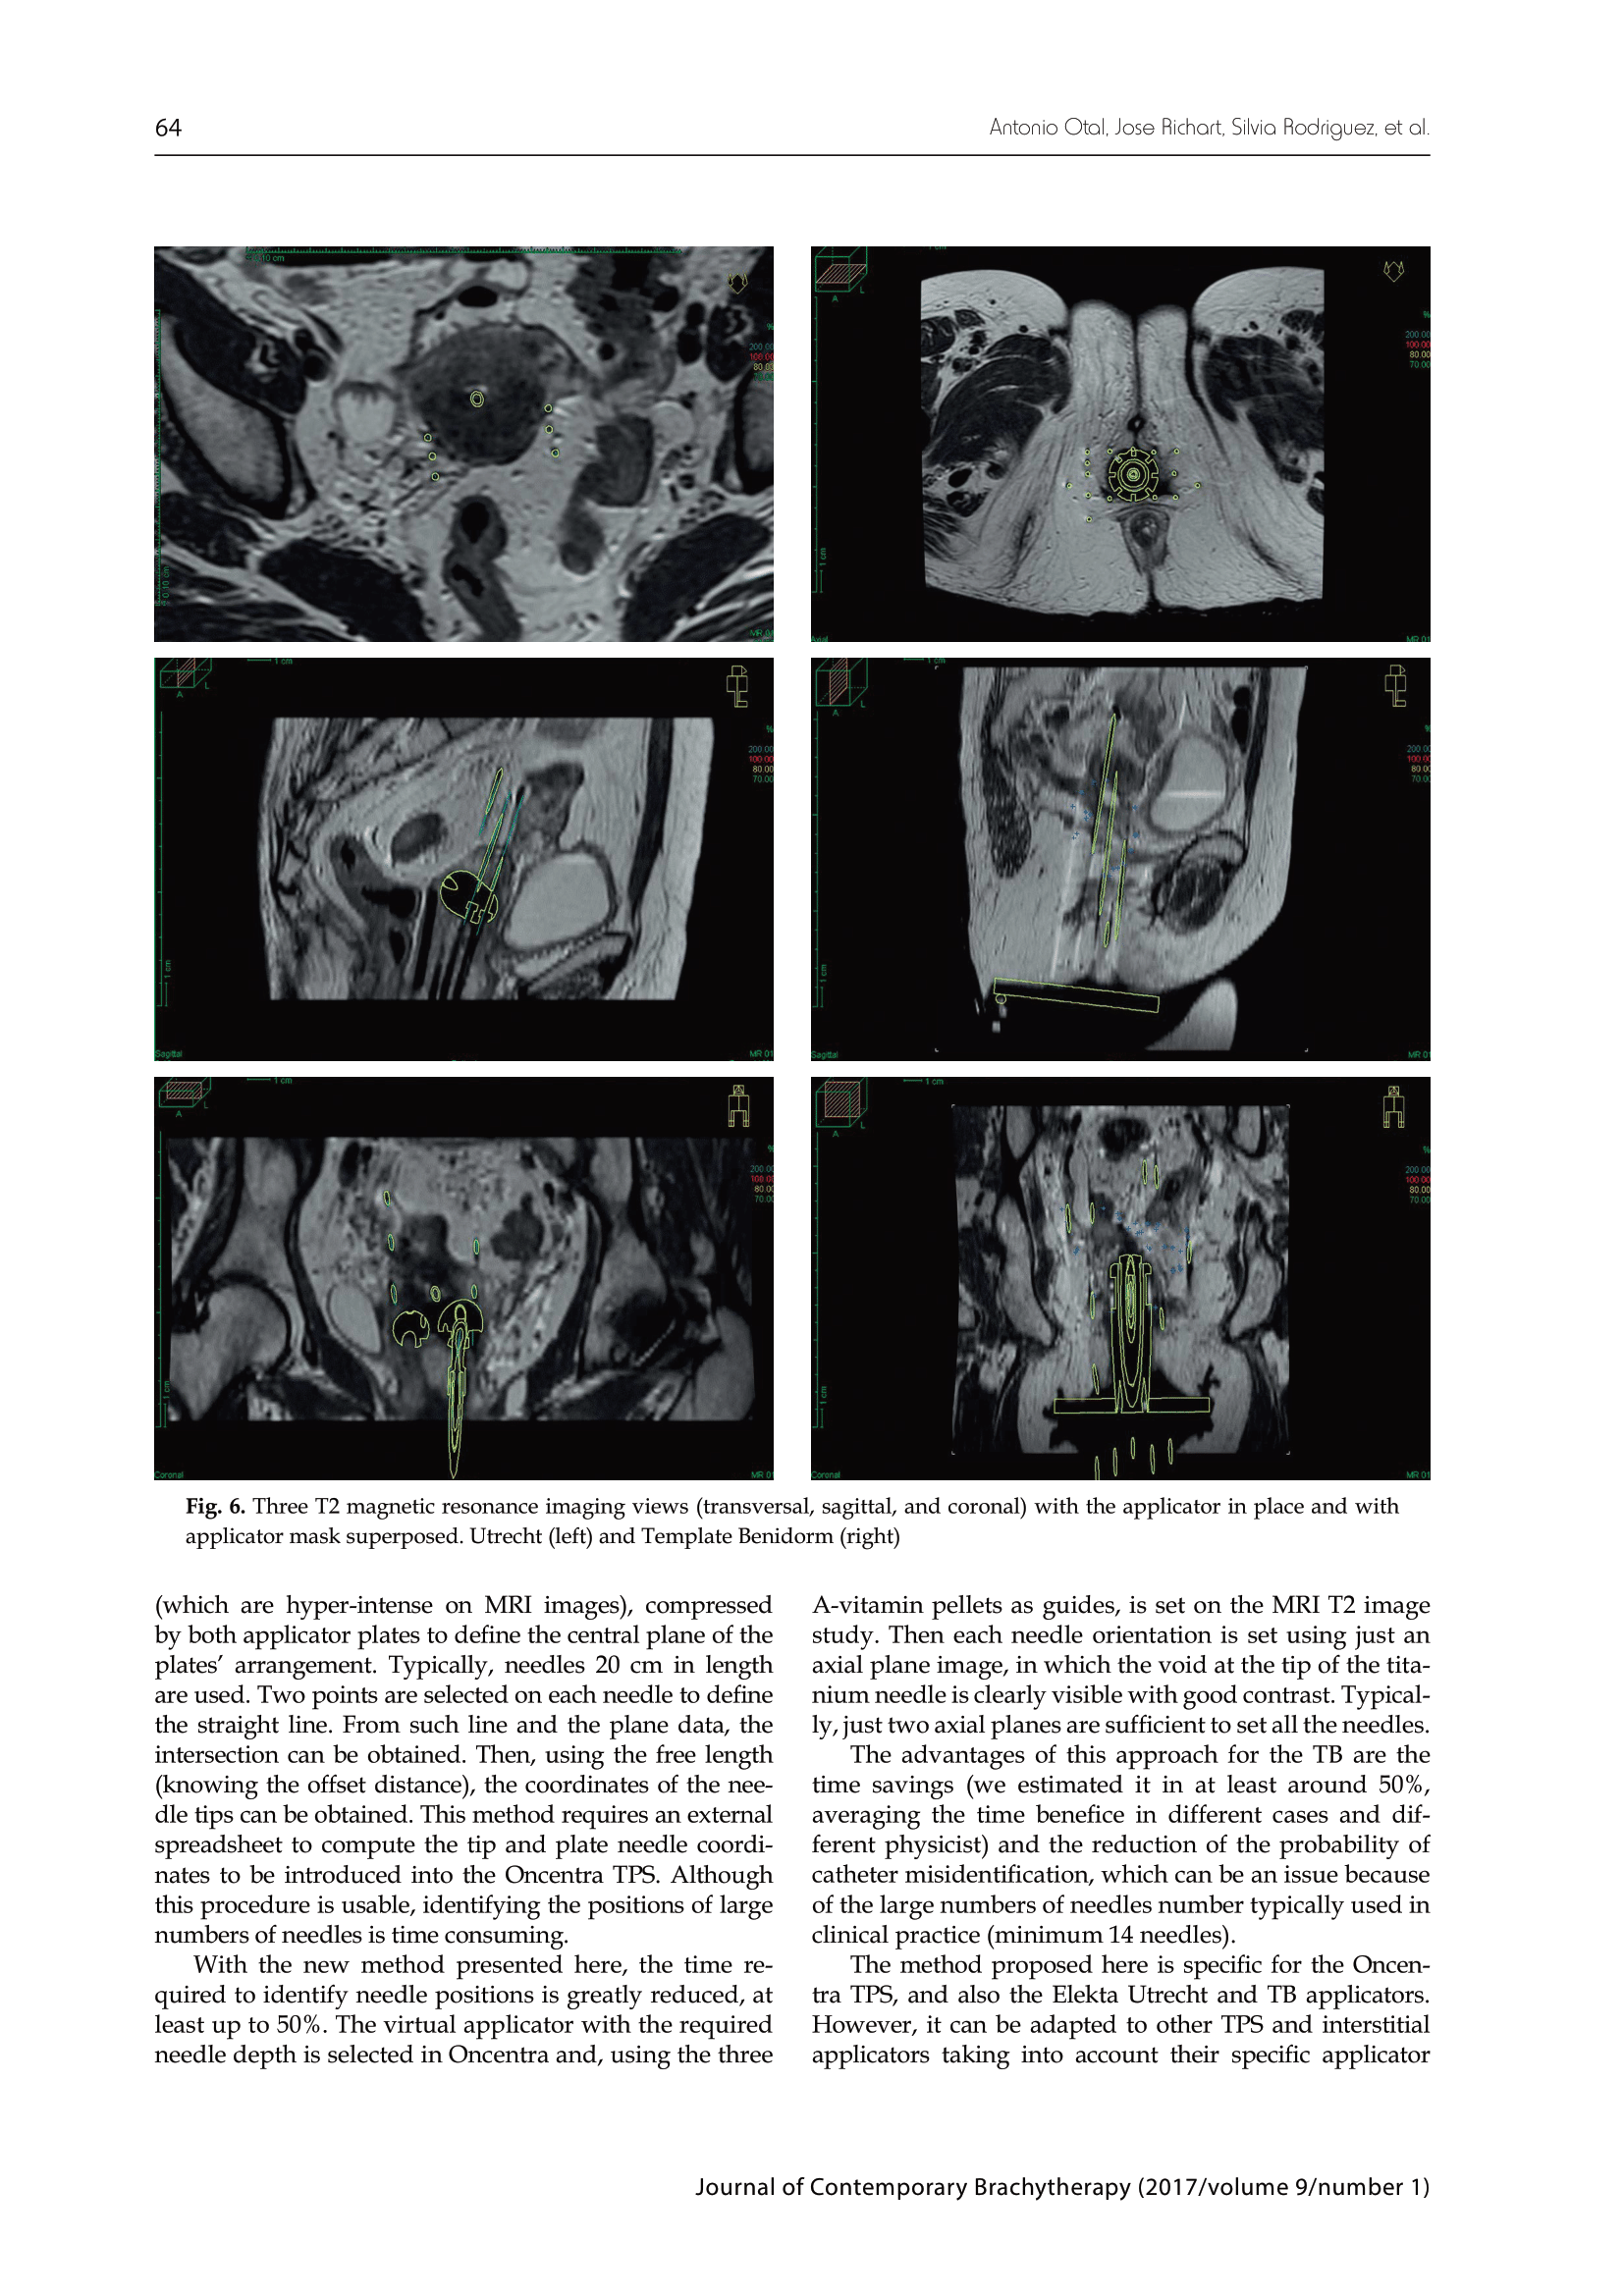
\includegraphics{articulos/librerias/librerias-6.png}
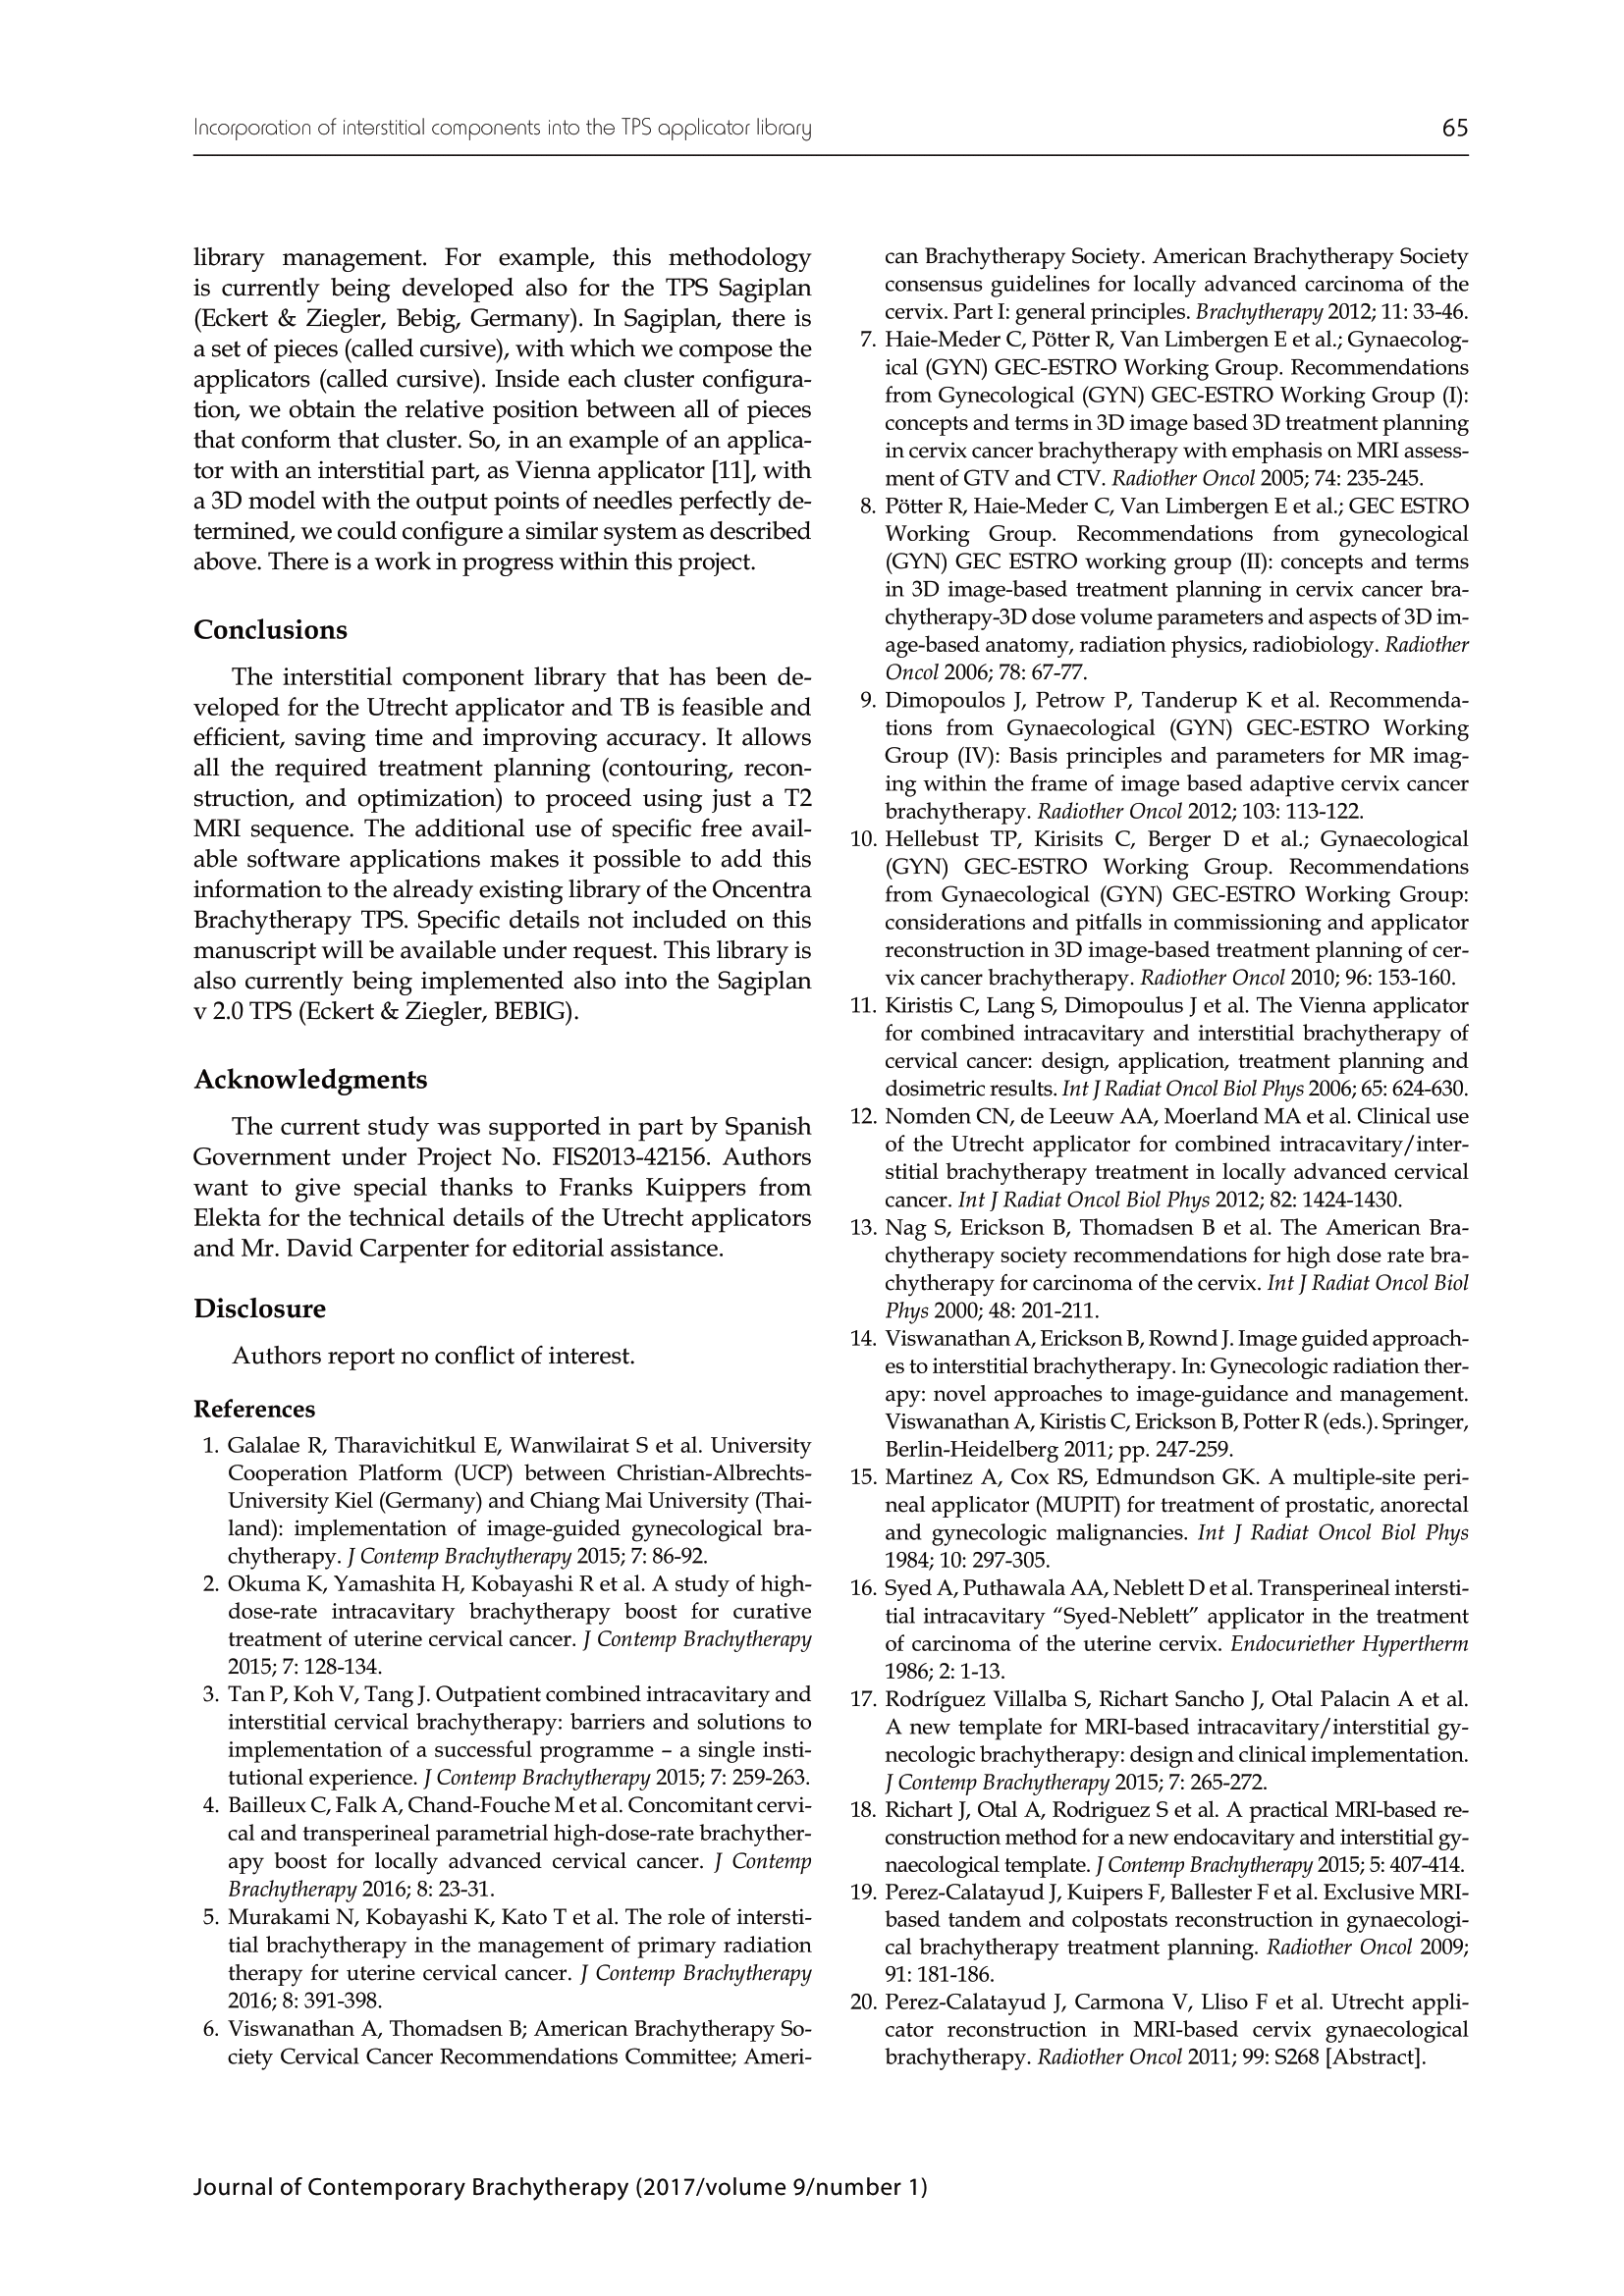
\includegraphics{articulos/librerias/librerias-7.png}

\hypertarget{pre-plan-technique-feasibility-in-multi-interstitialendocavitary-perineal-gynecological-brachytherapy.}{%
\section{Pre-plan technique feasibility in
multi-interstitial/endocavitary perineal gynecological
brachytherapy.}\label{pre-plan-technique-feasibility-in-multi-interstitialendocavitary-perineal-gynecological-brachytherapy.}}

\newpage{}

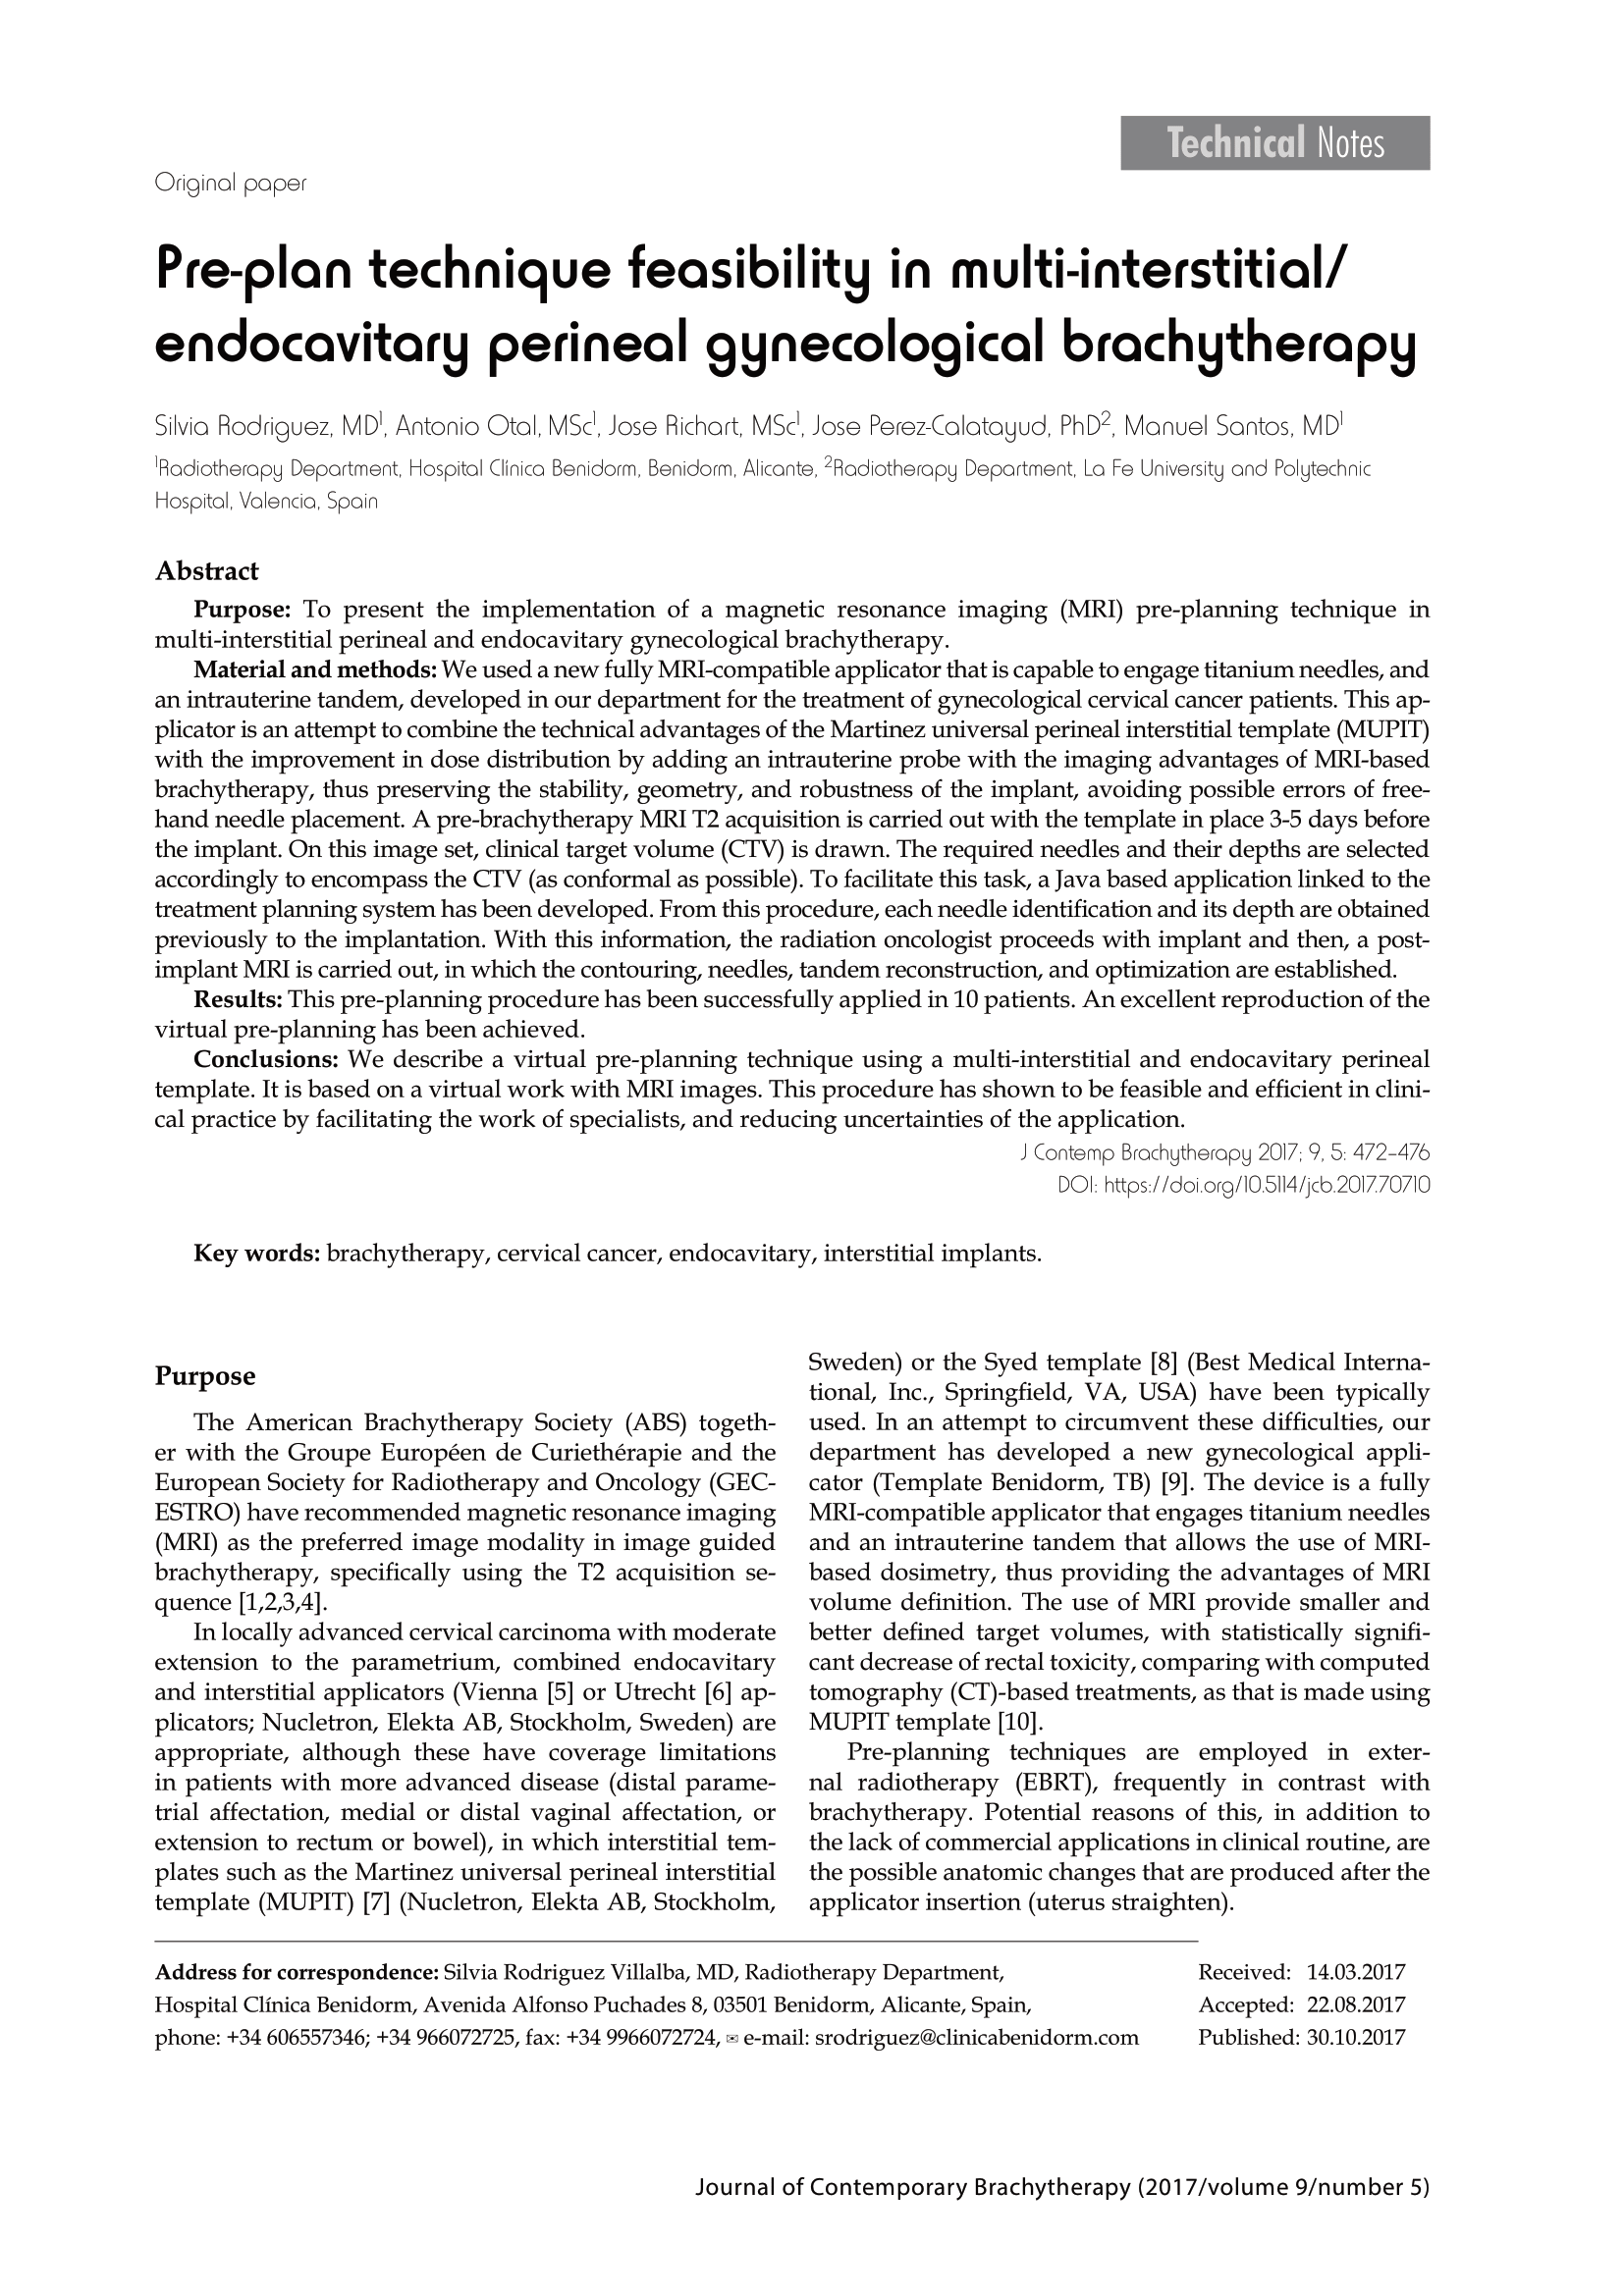
\includegraphics{articulos/preplan/preplan-1.png}
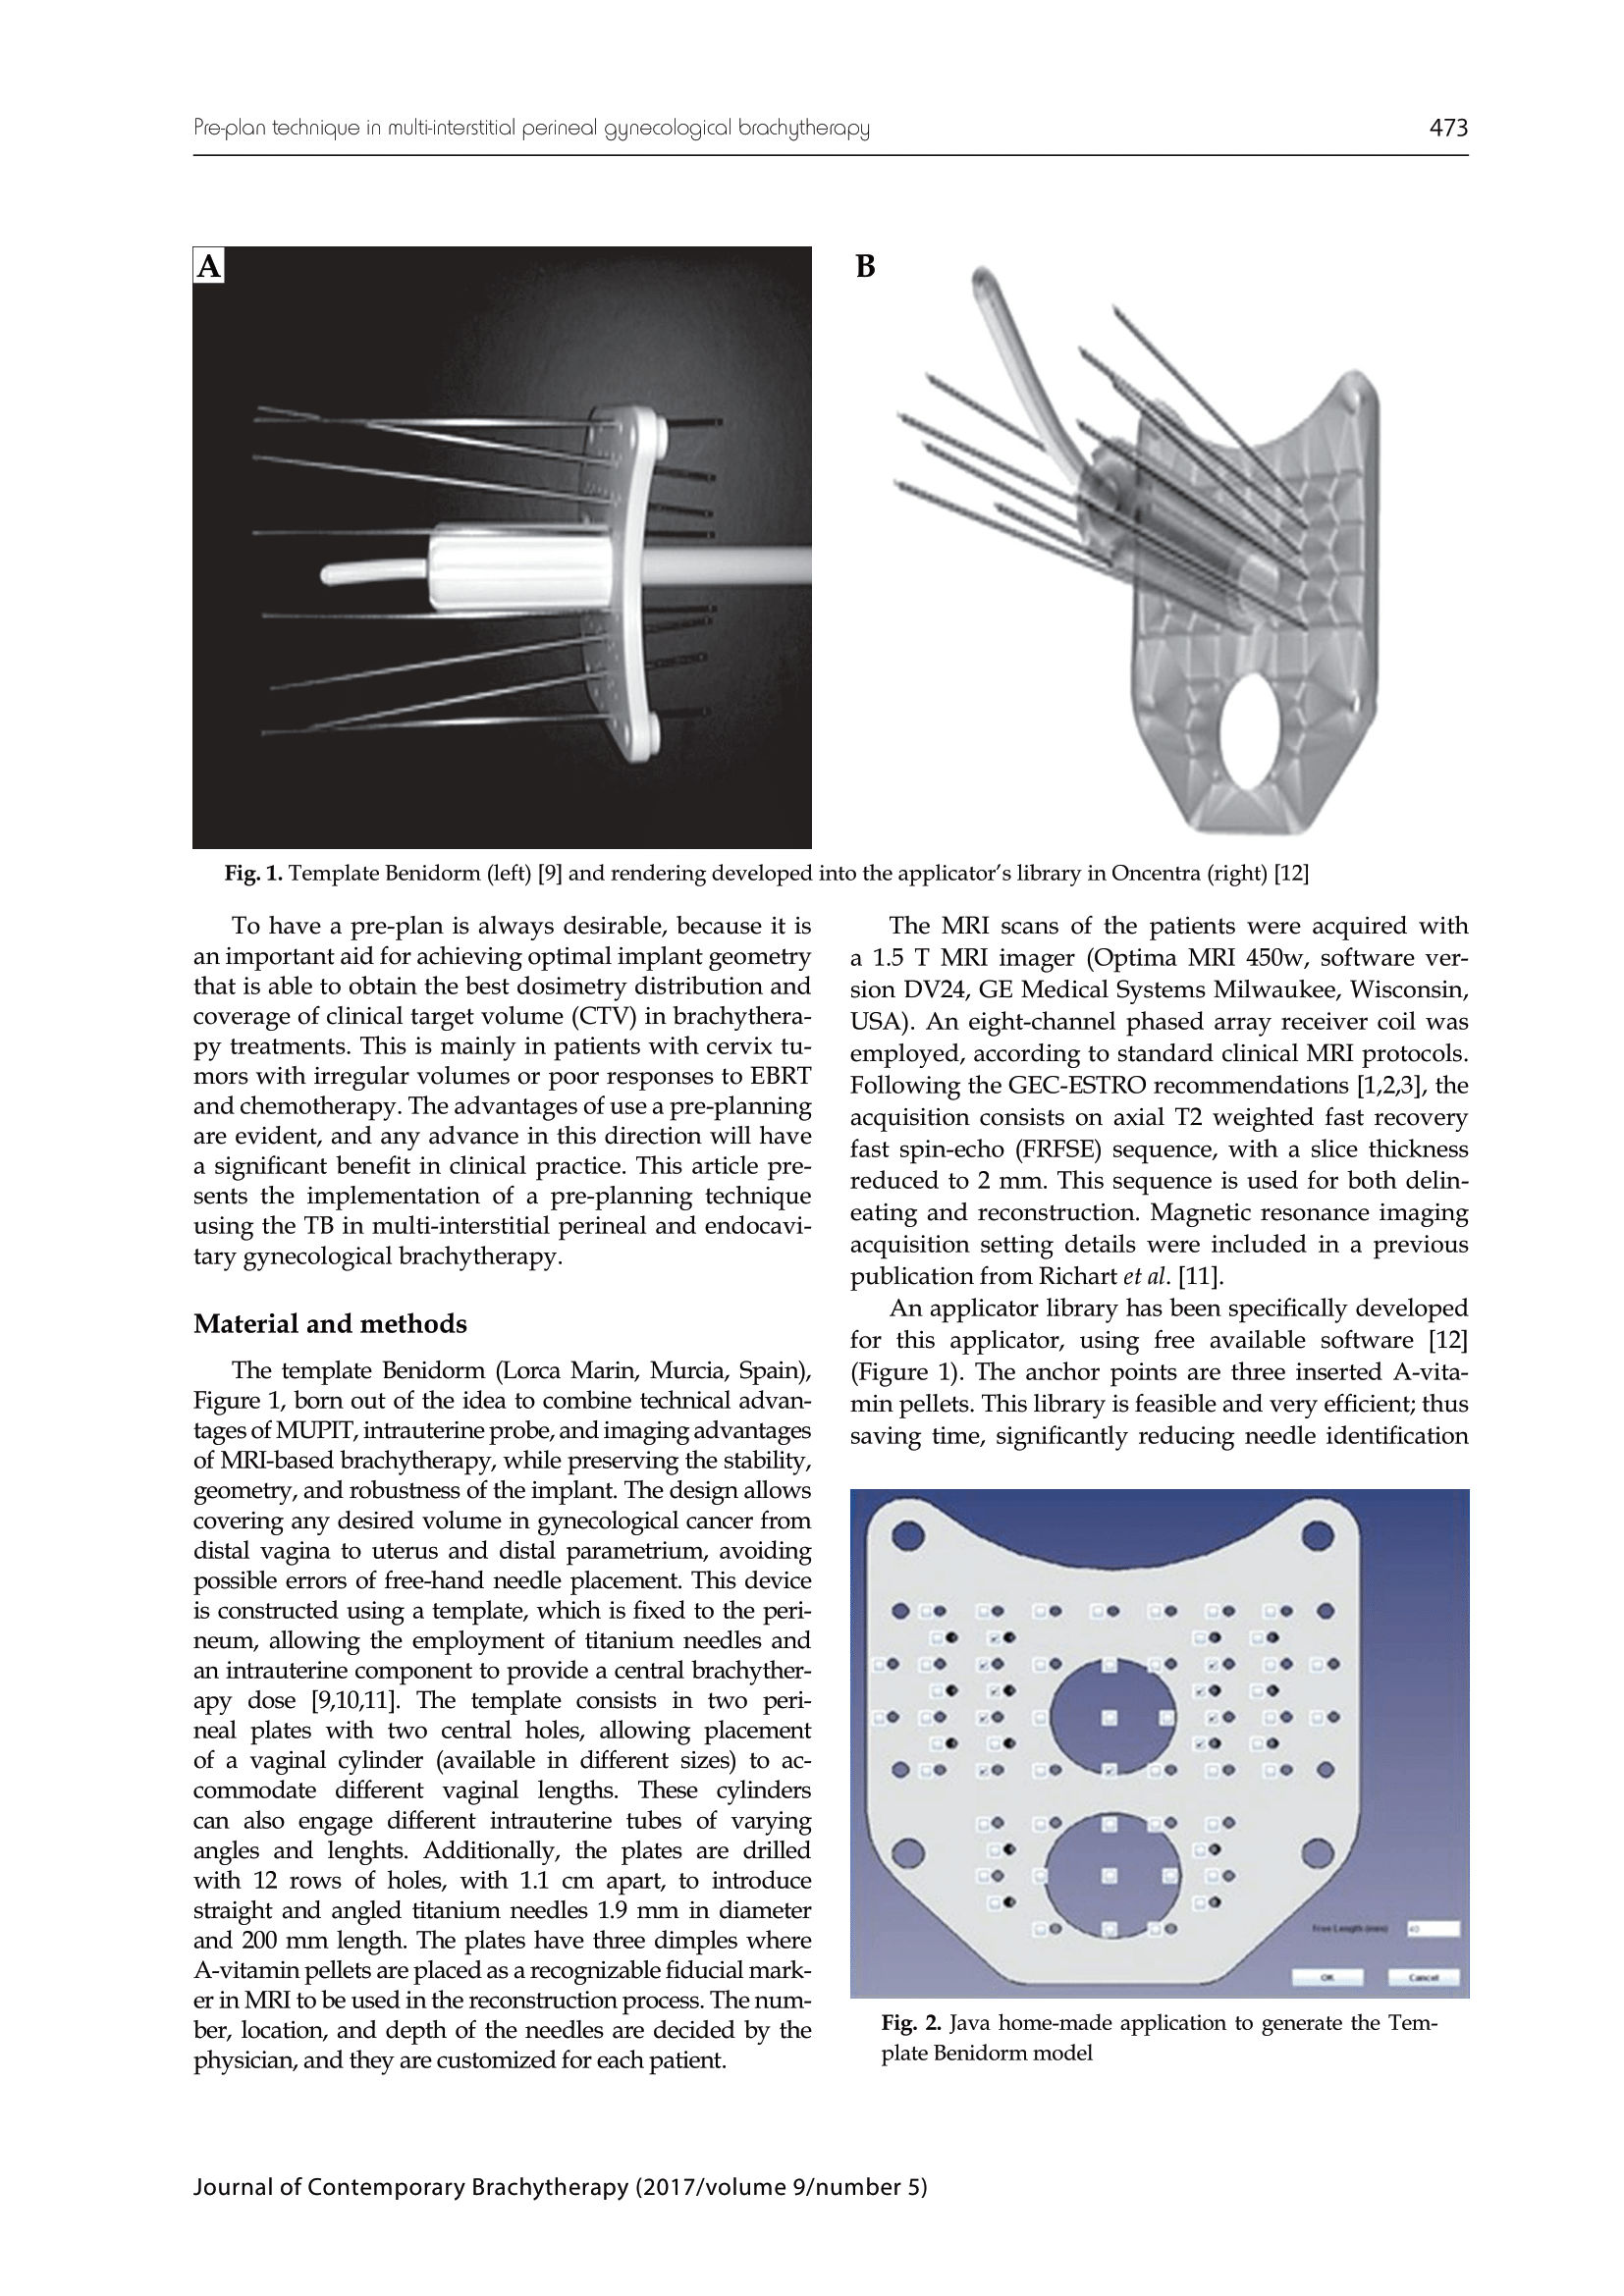
\includegraphics{articulos/preplan/preplan-2.png}
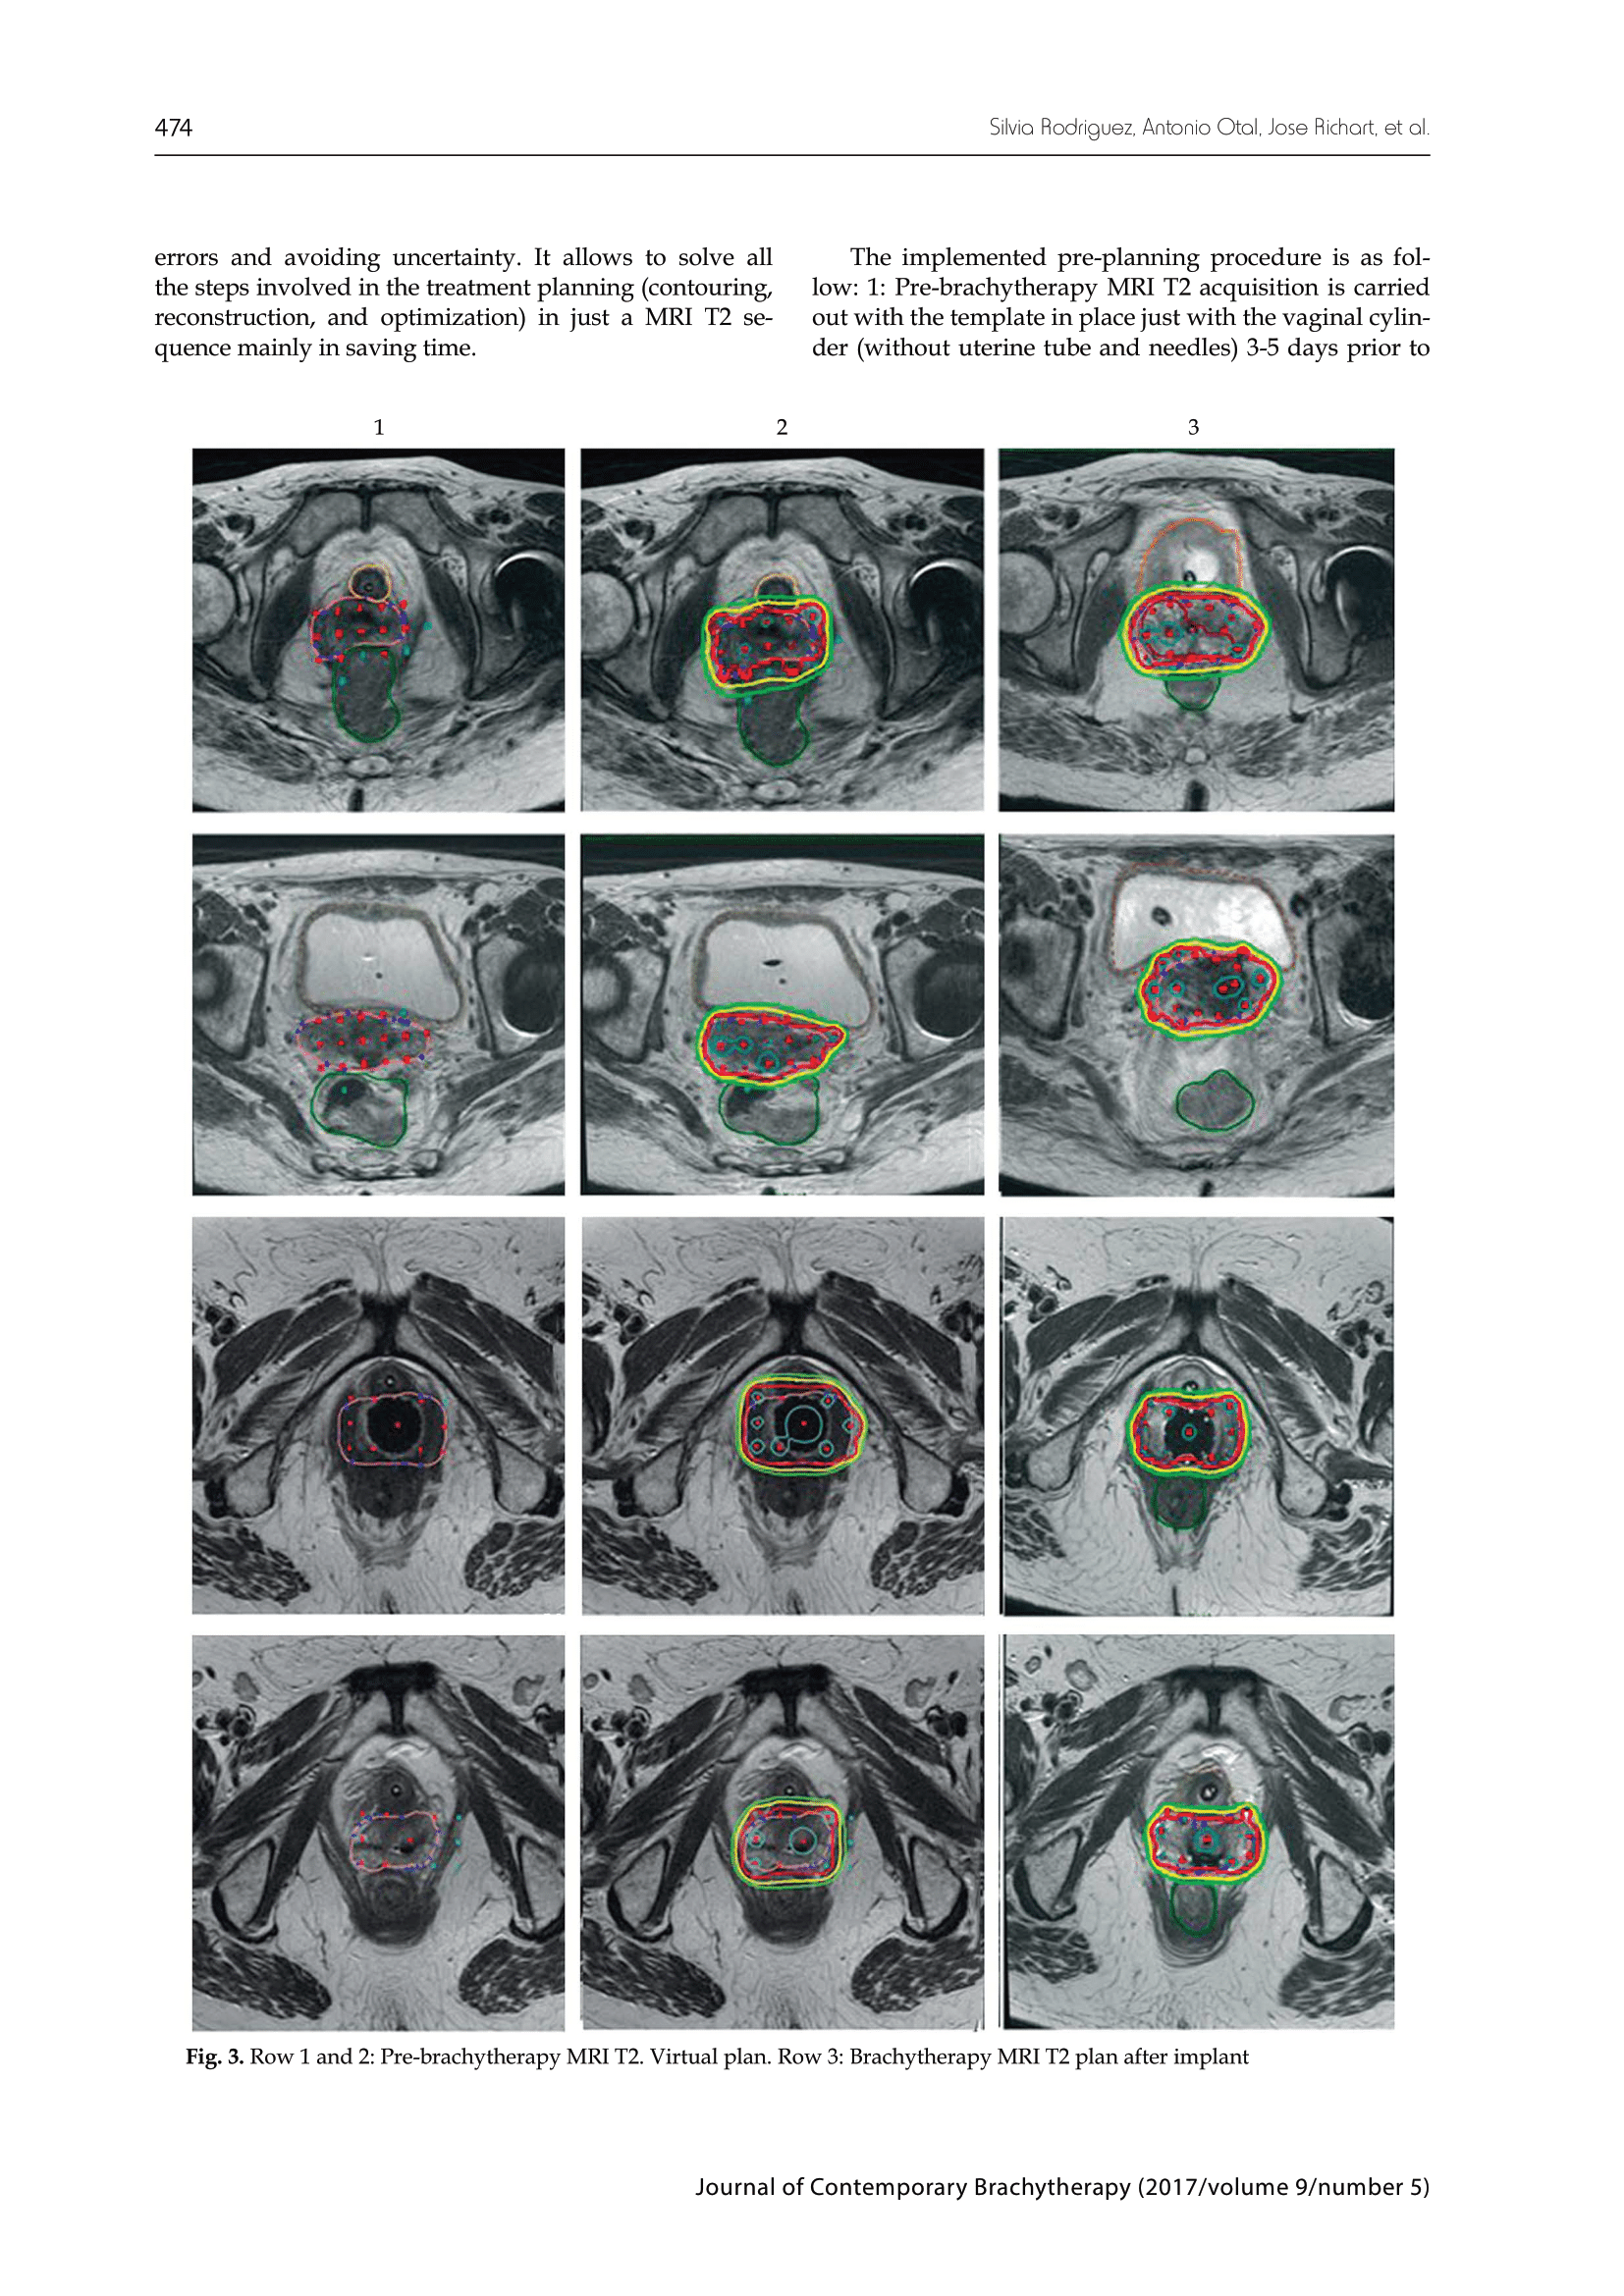
\includegraphics{articulos/preplan/preplan-3.png}
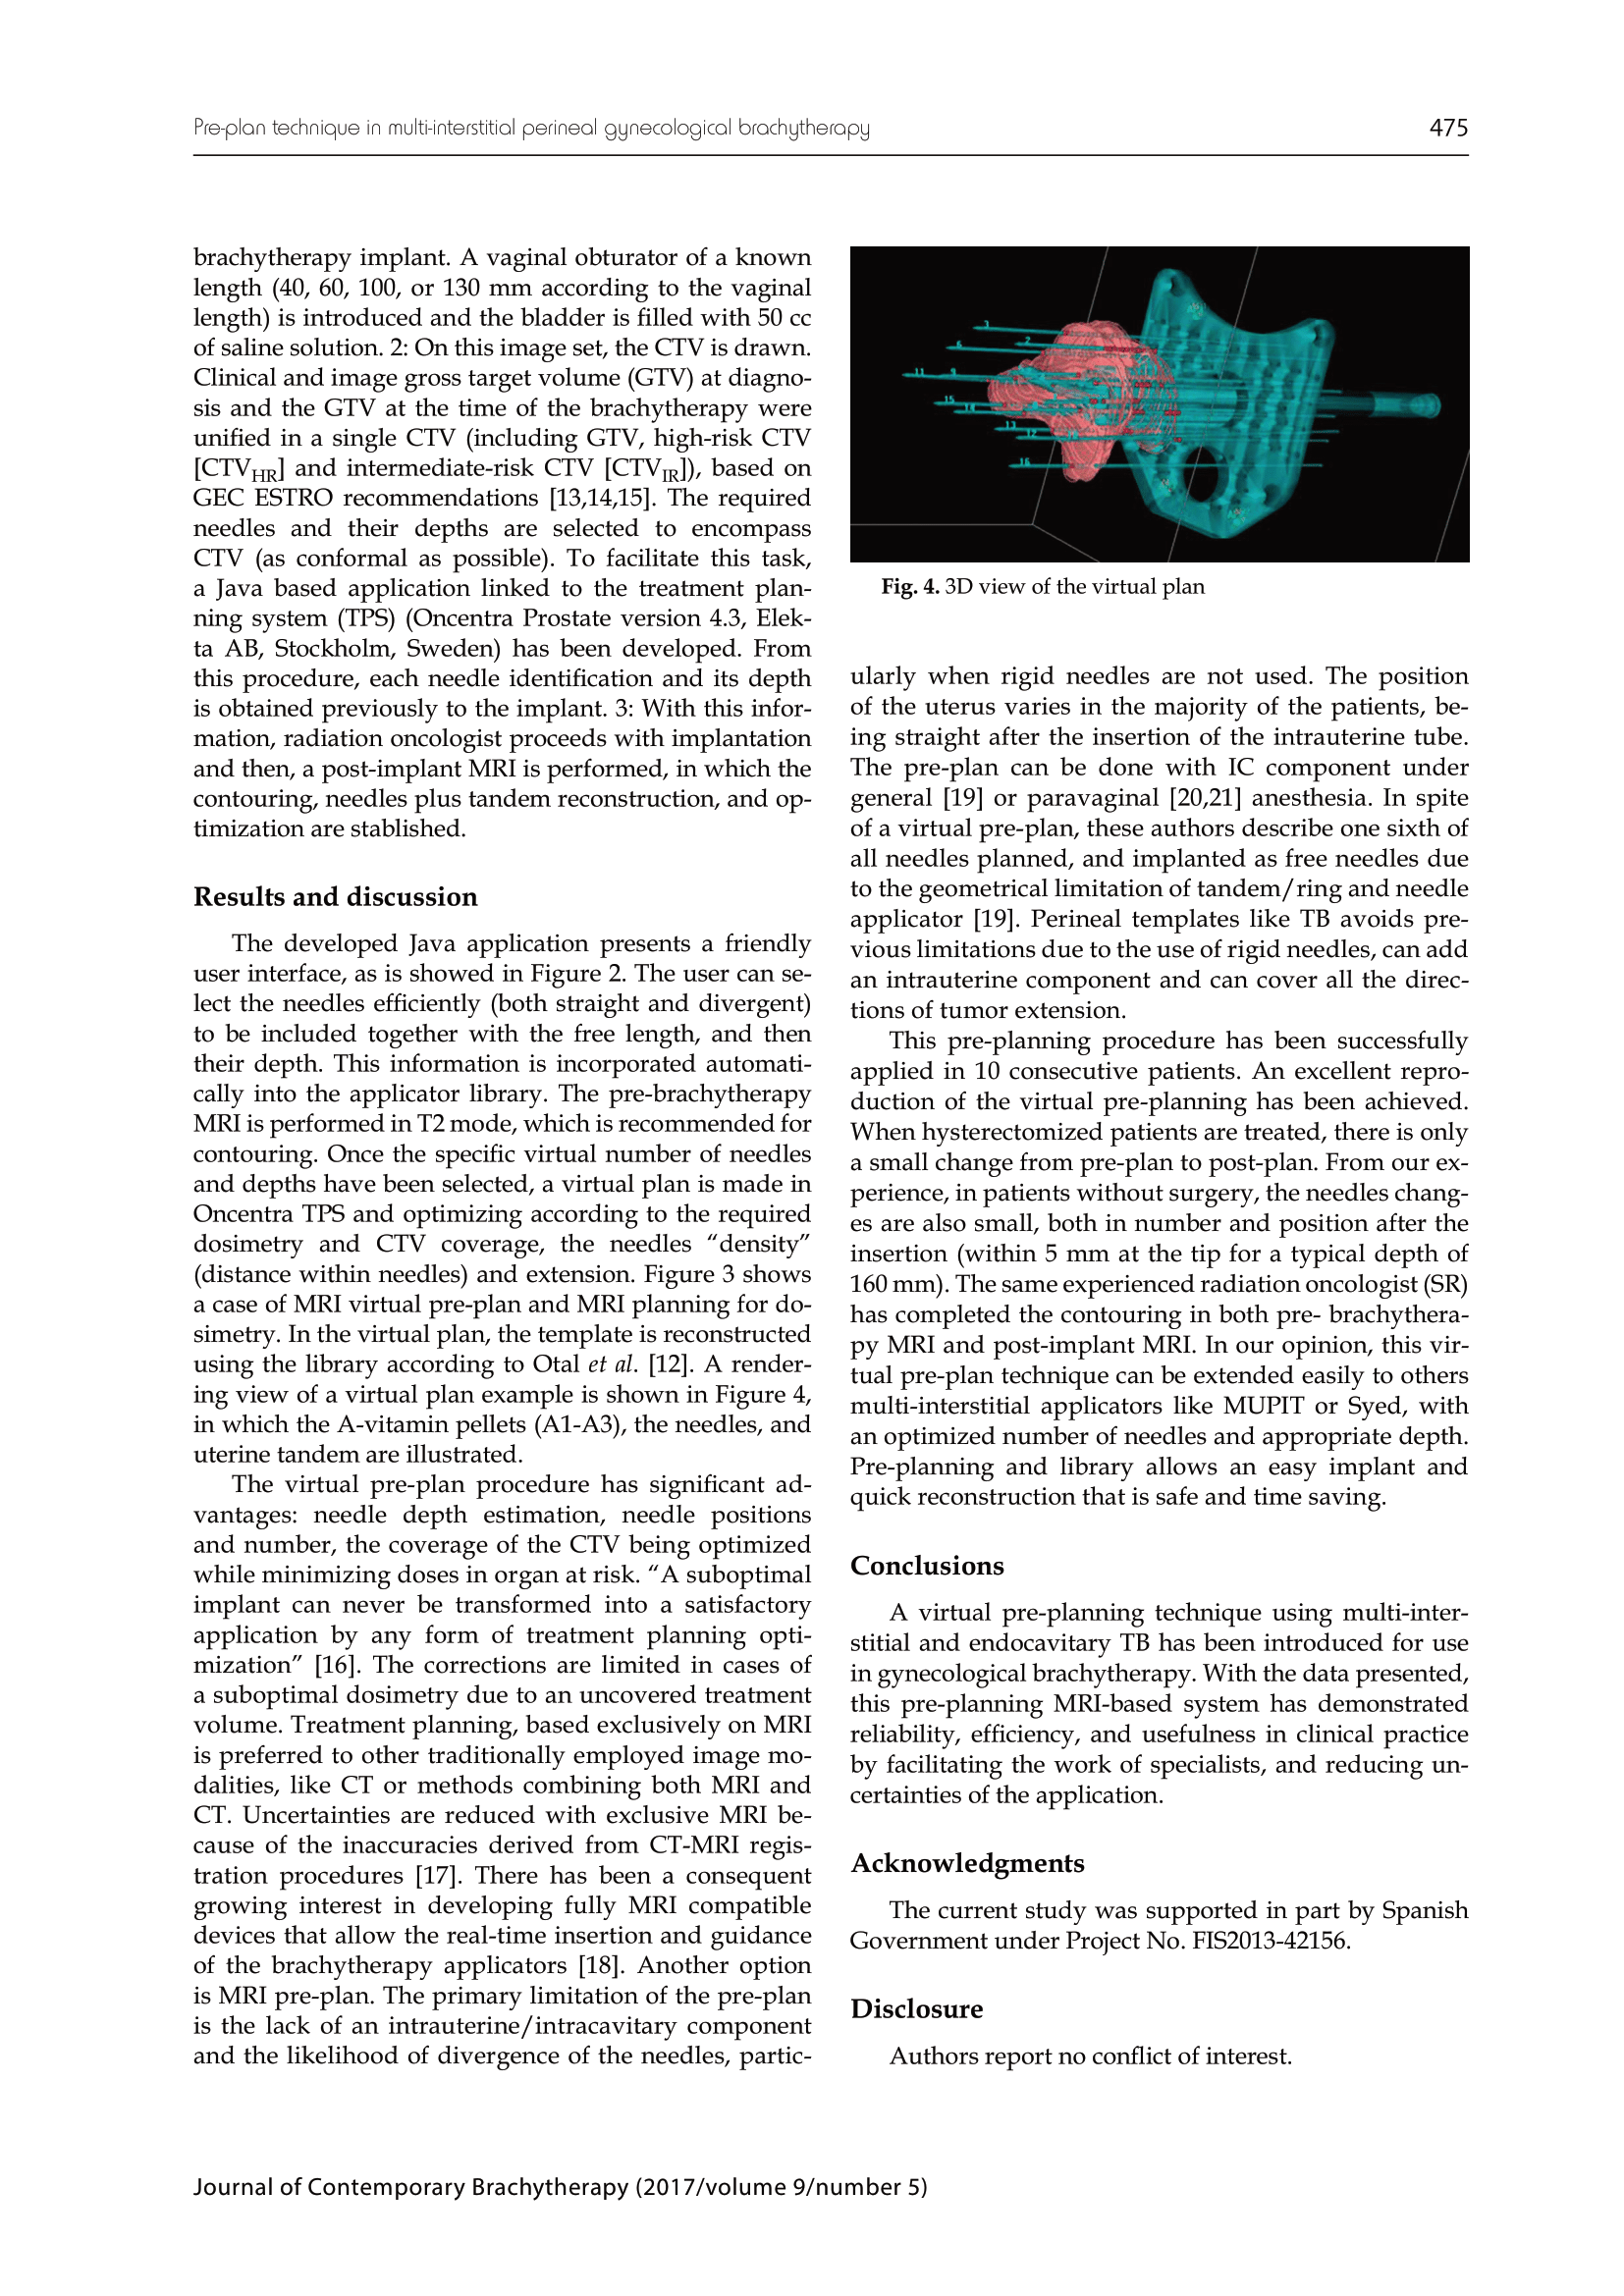
\includegraphics{articulos/preplan/preplan-4.png}
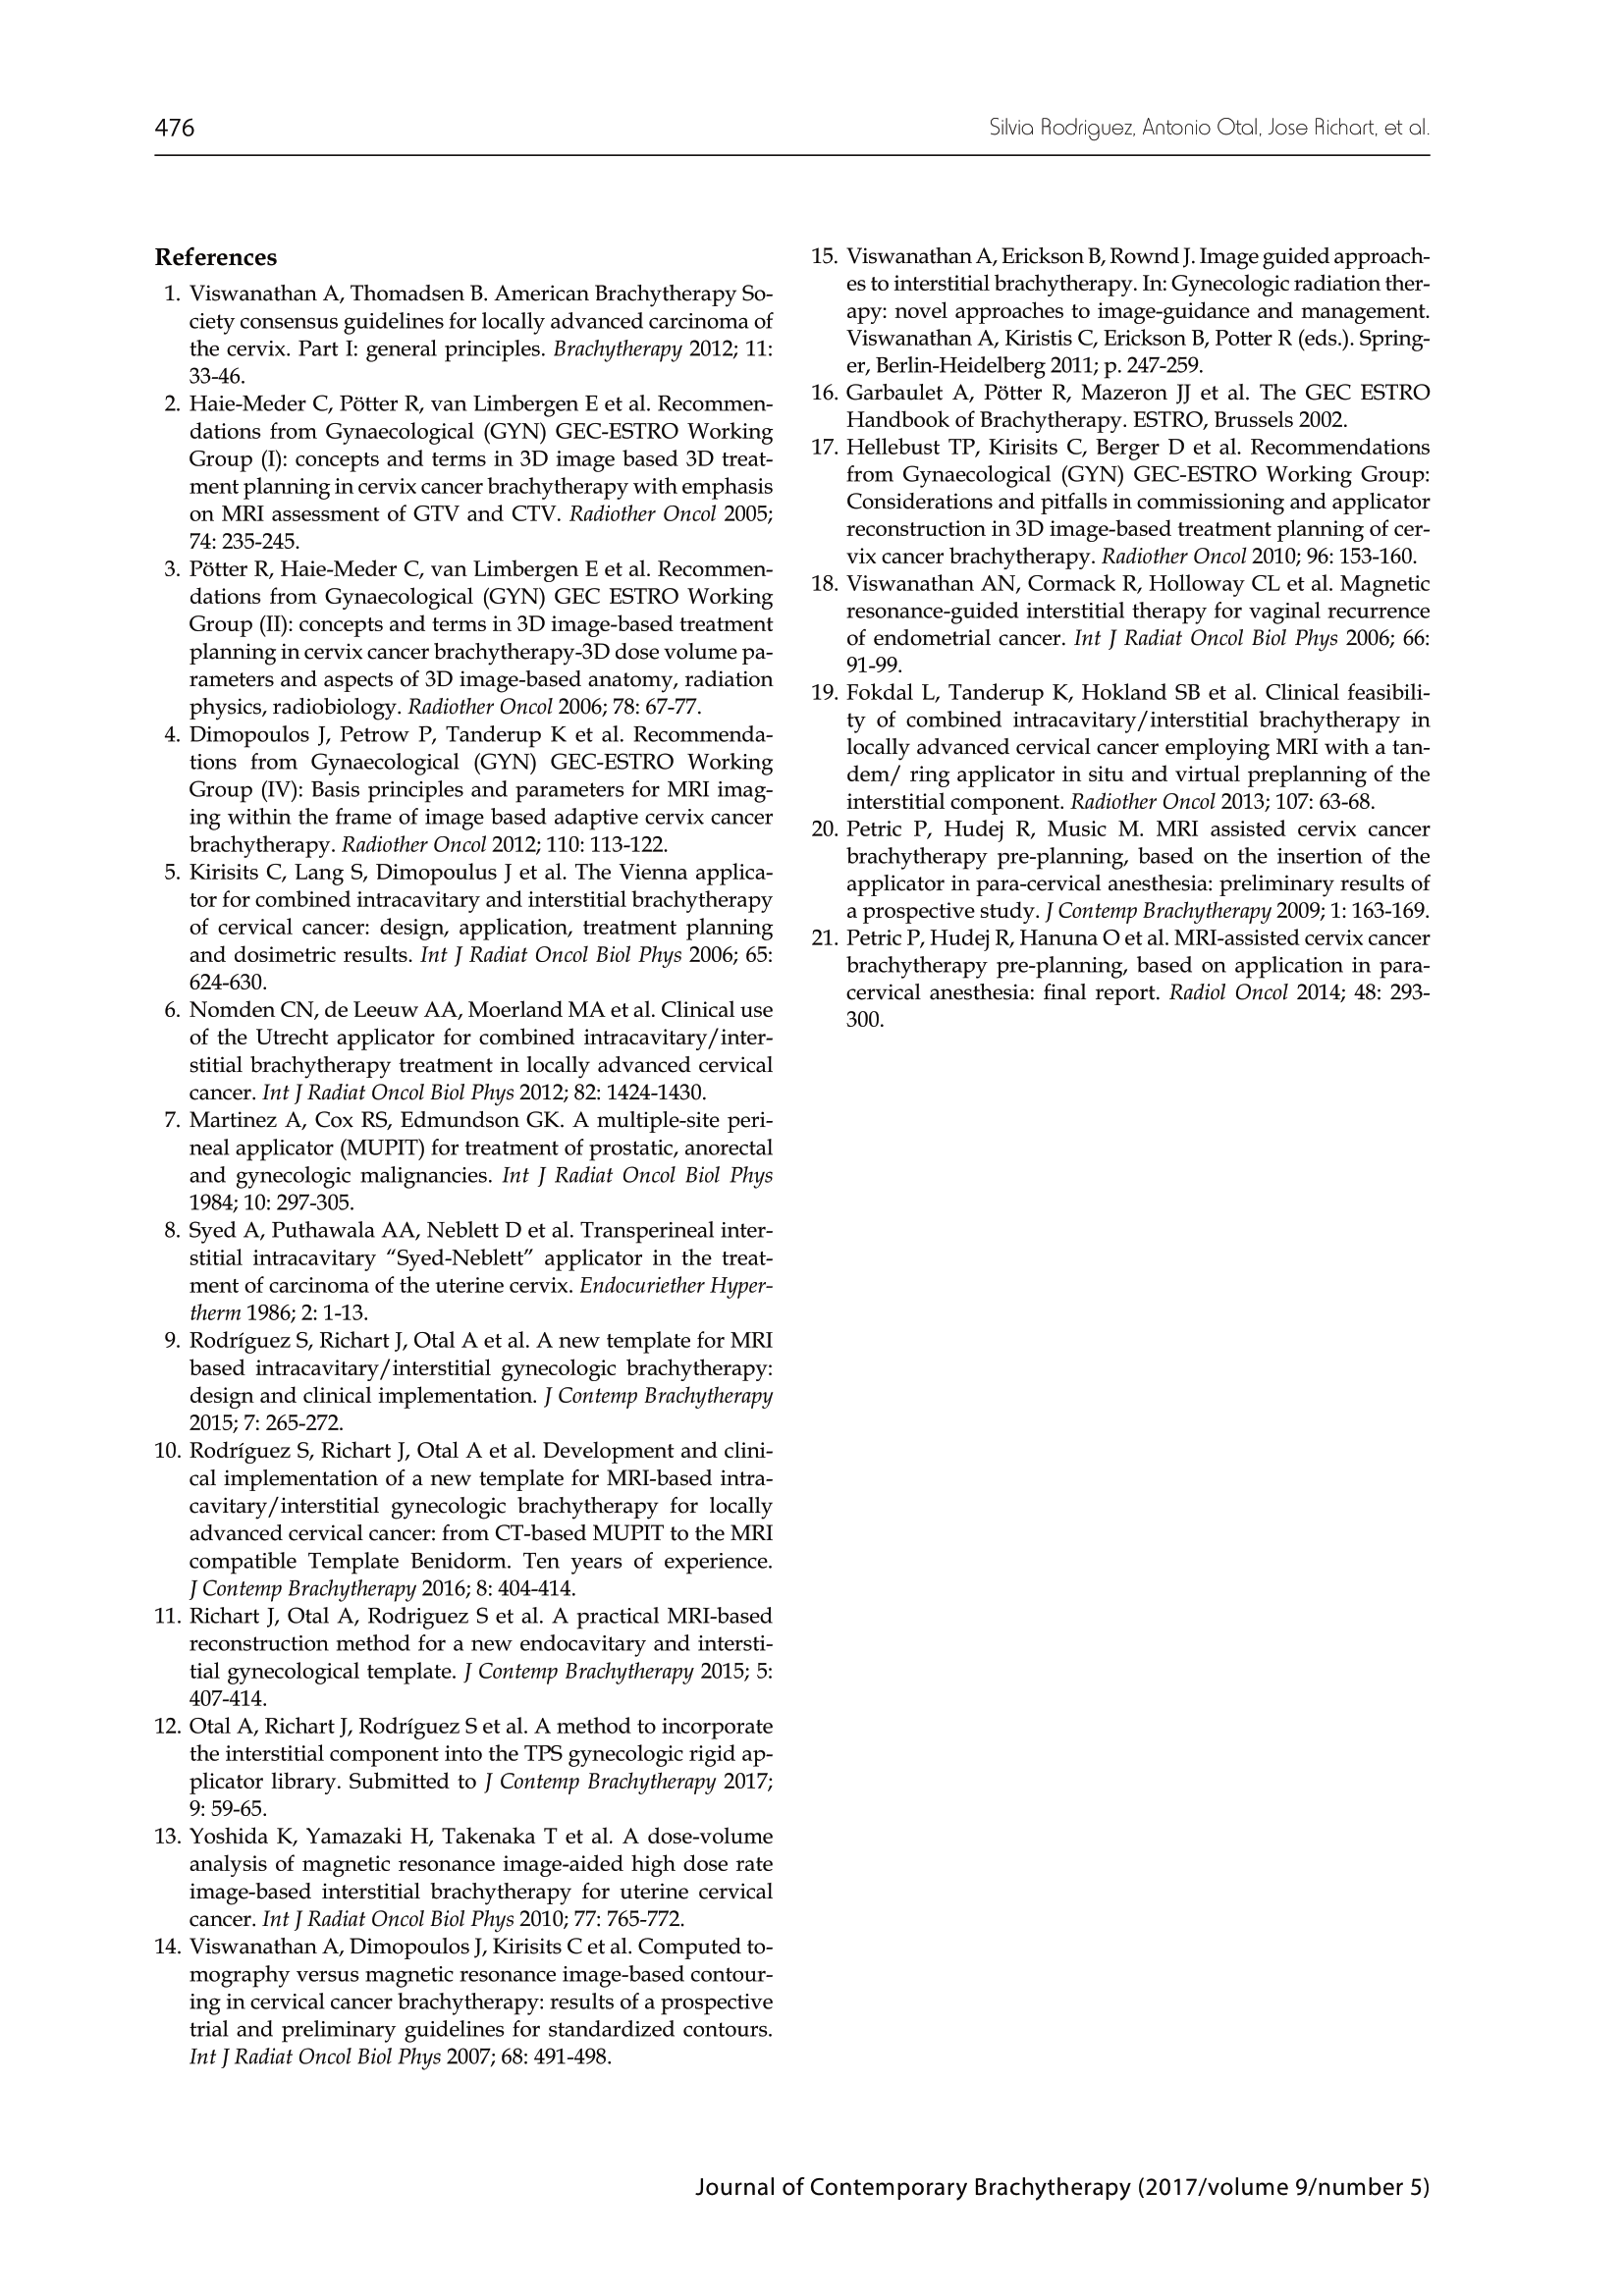
\includegraphics{articulos/preplan/preplan-5.png}

\hypertarget{review-on-treatment-planning-systems-for-cervix-brachytherapy-interventional-radiotherapy-some-desirable-and-convenient-practical-aspects-to-be-implemented-from-radiation-oncologist-and-medical-physics-perspectives.}{%
\section{Review on Treatment Planning Systems for Cervix Brachytherapy
(Interventional Radiotherapy): Some Desirable and Convenient Practical
Aspects to Be Implemented from Radiation Oncologist and Medical Physics
Perspectives.}\label{review-on-treatment-planning-systems-for-cervix-brachytherapy-interventional-radiotherapy-some-desirable-and-convenient-practical-aspects-to-be-implemented-from-radiation-oncologist-and-medical-physics-perspectives.}}

\newpage{}

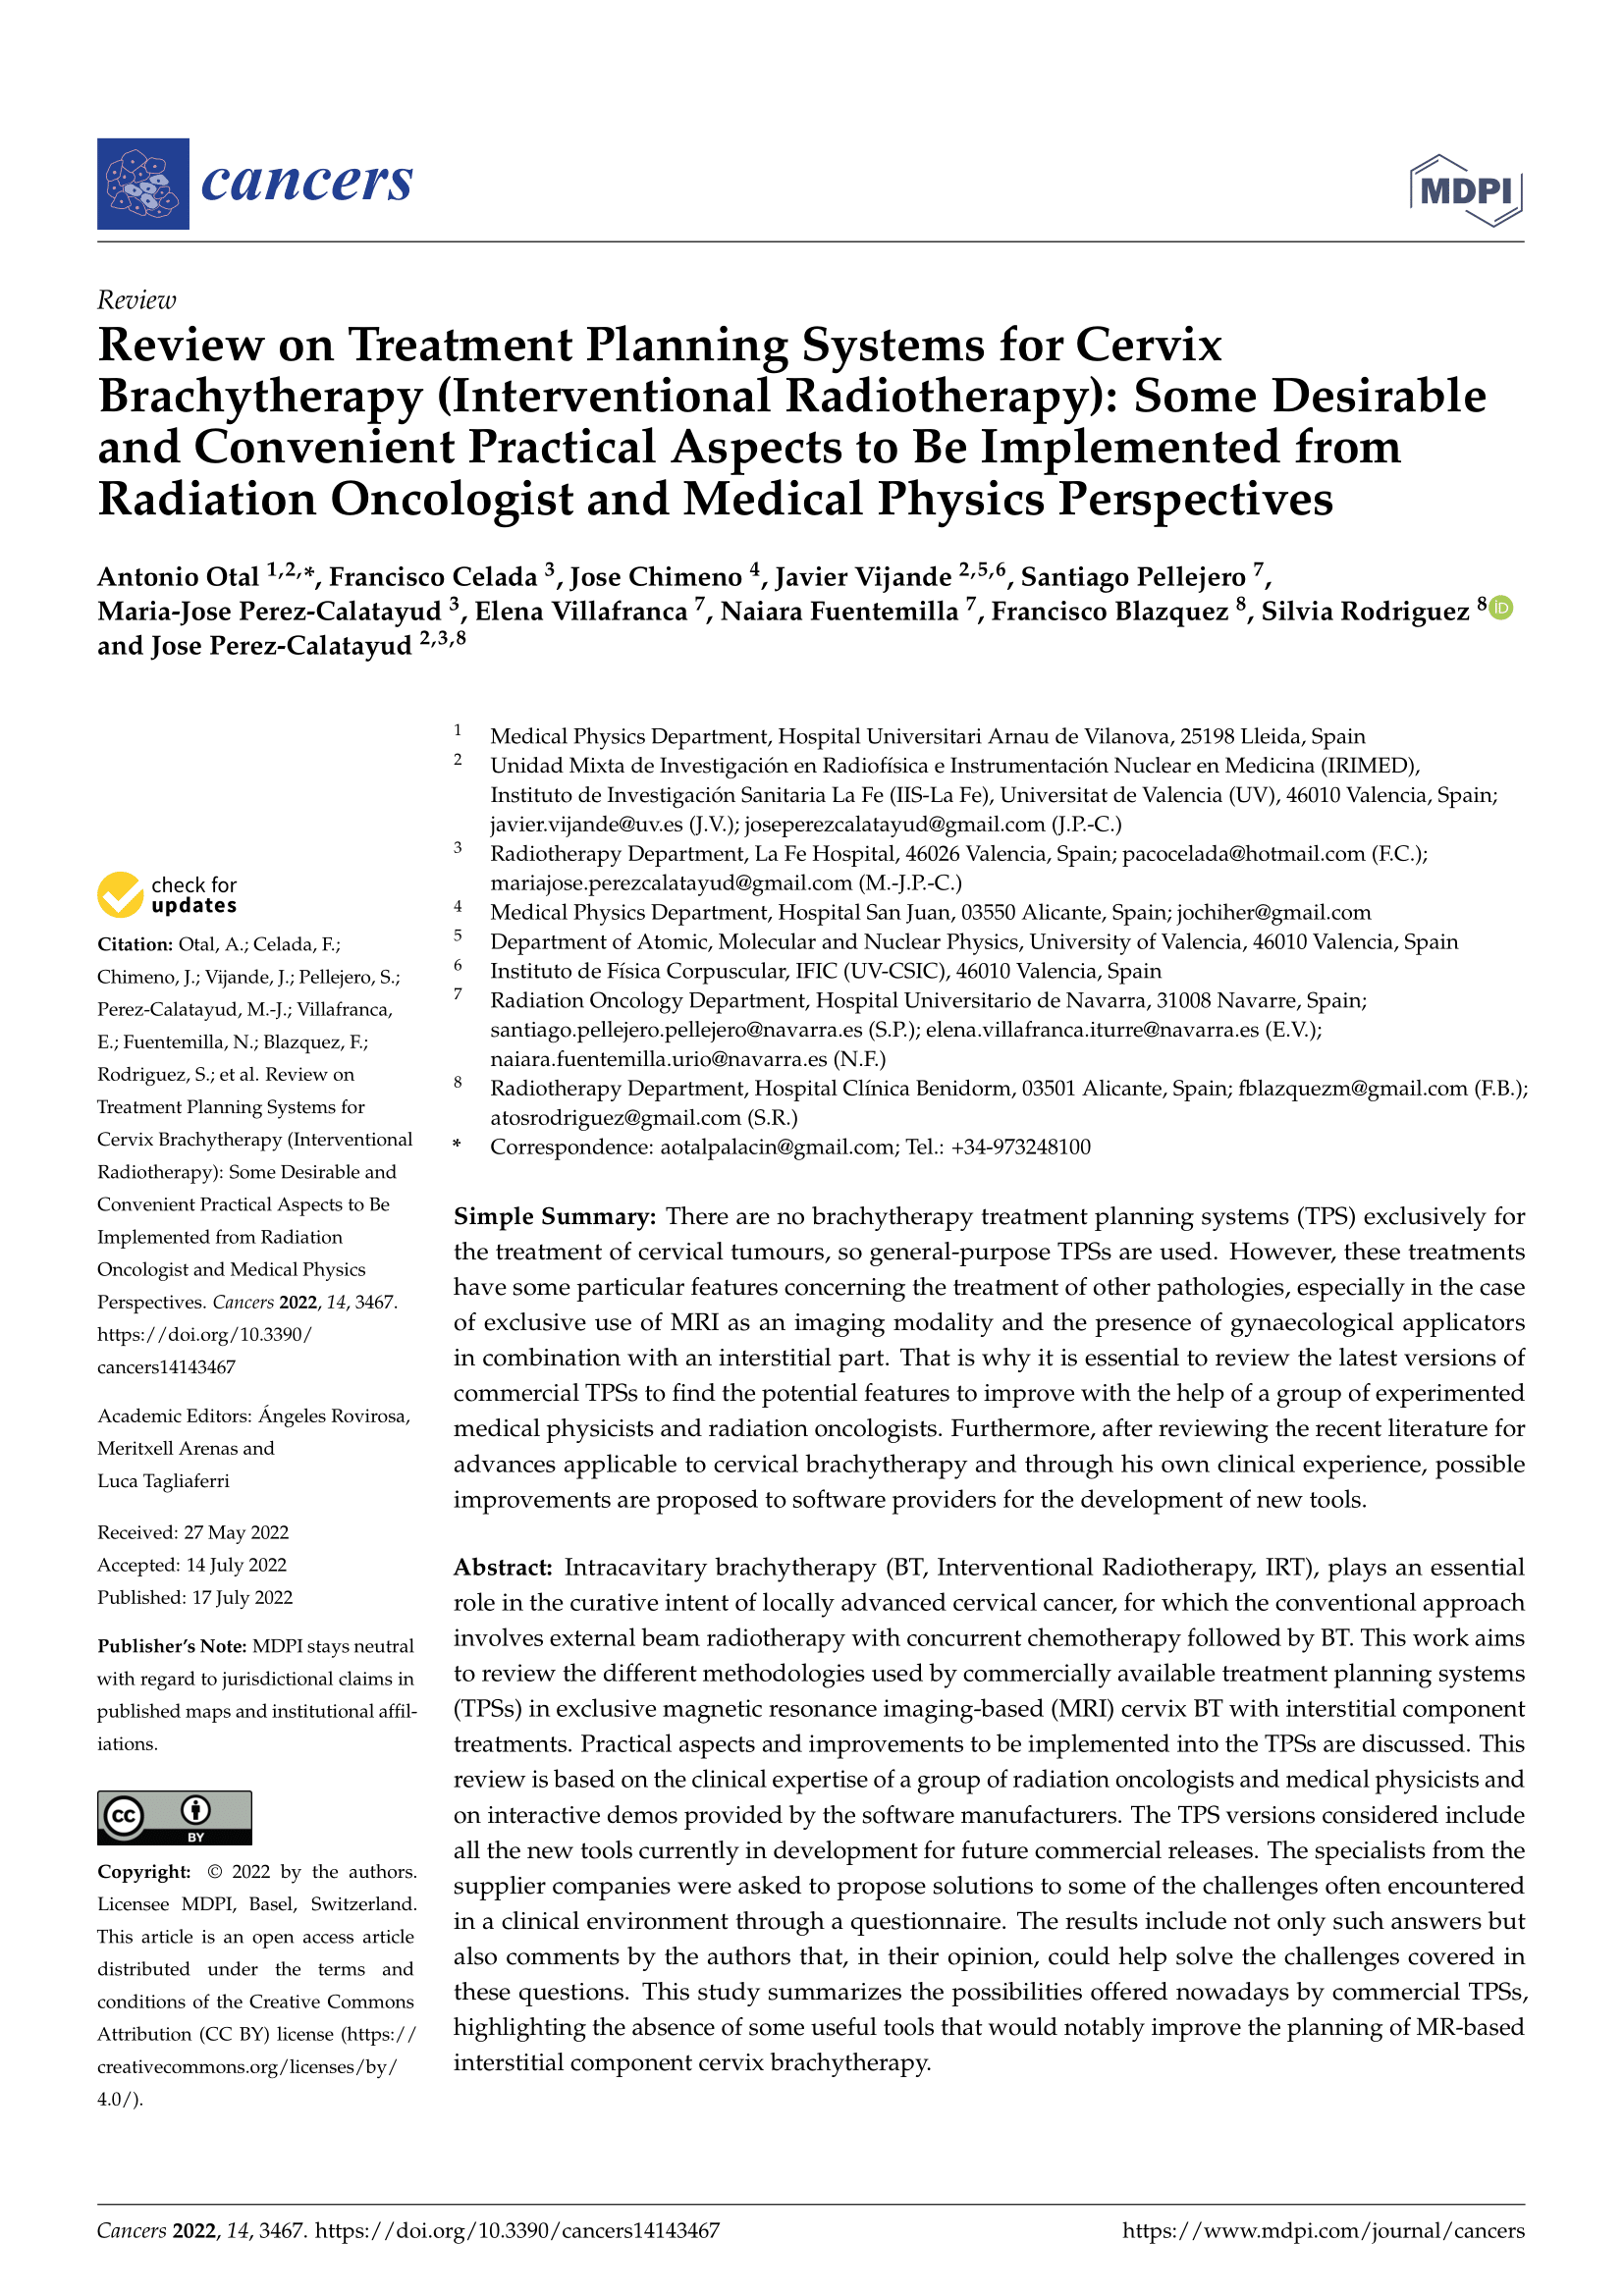
\includegraphics{articulos/cancers/cancers-01.png}
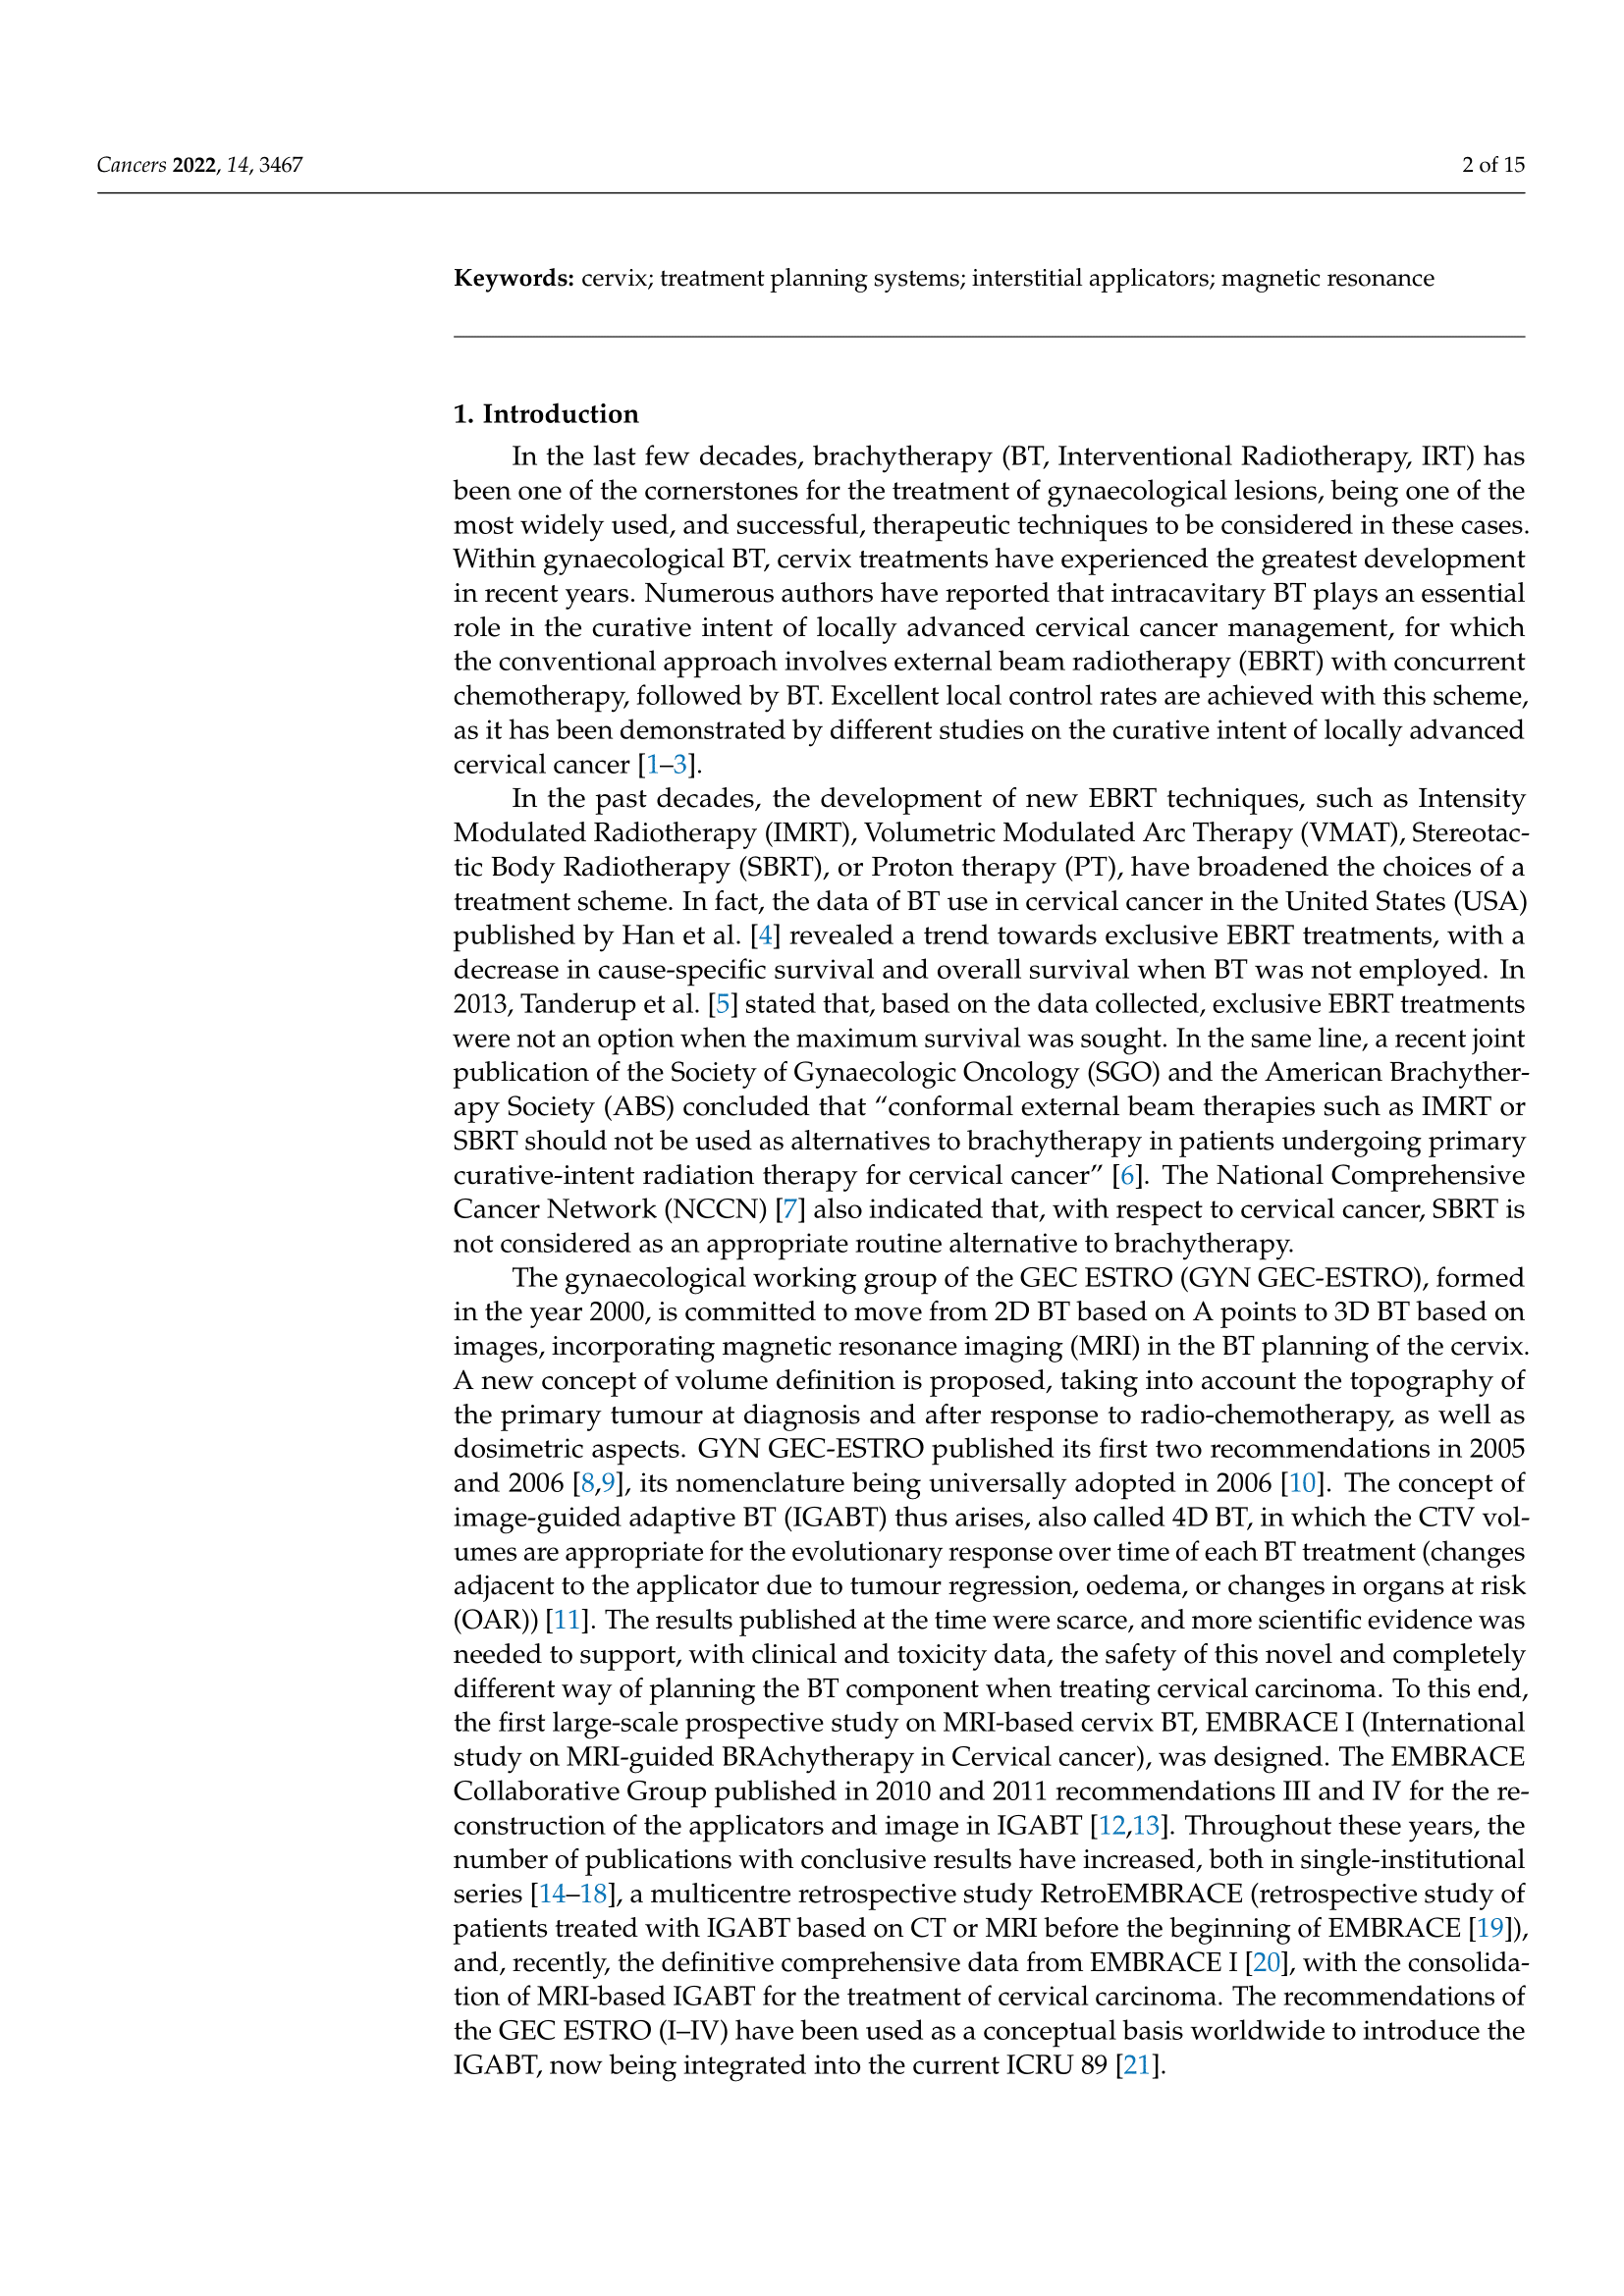
\includegraphics{articulos/cancers/cancers-02.png}
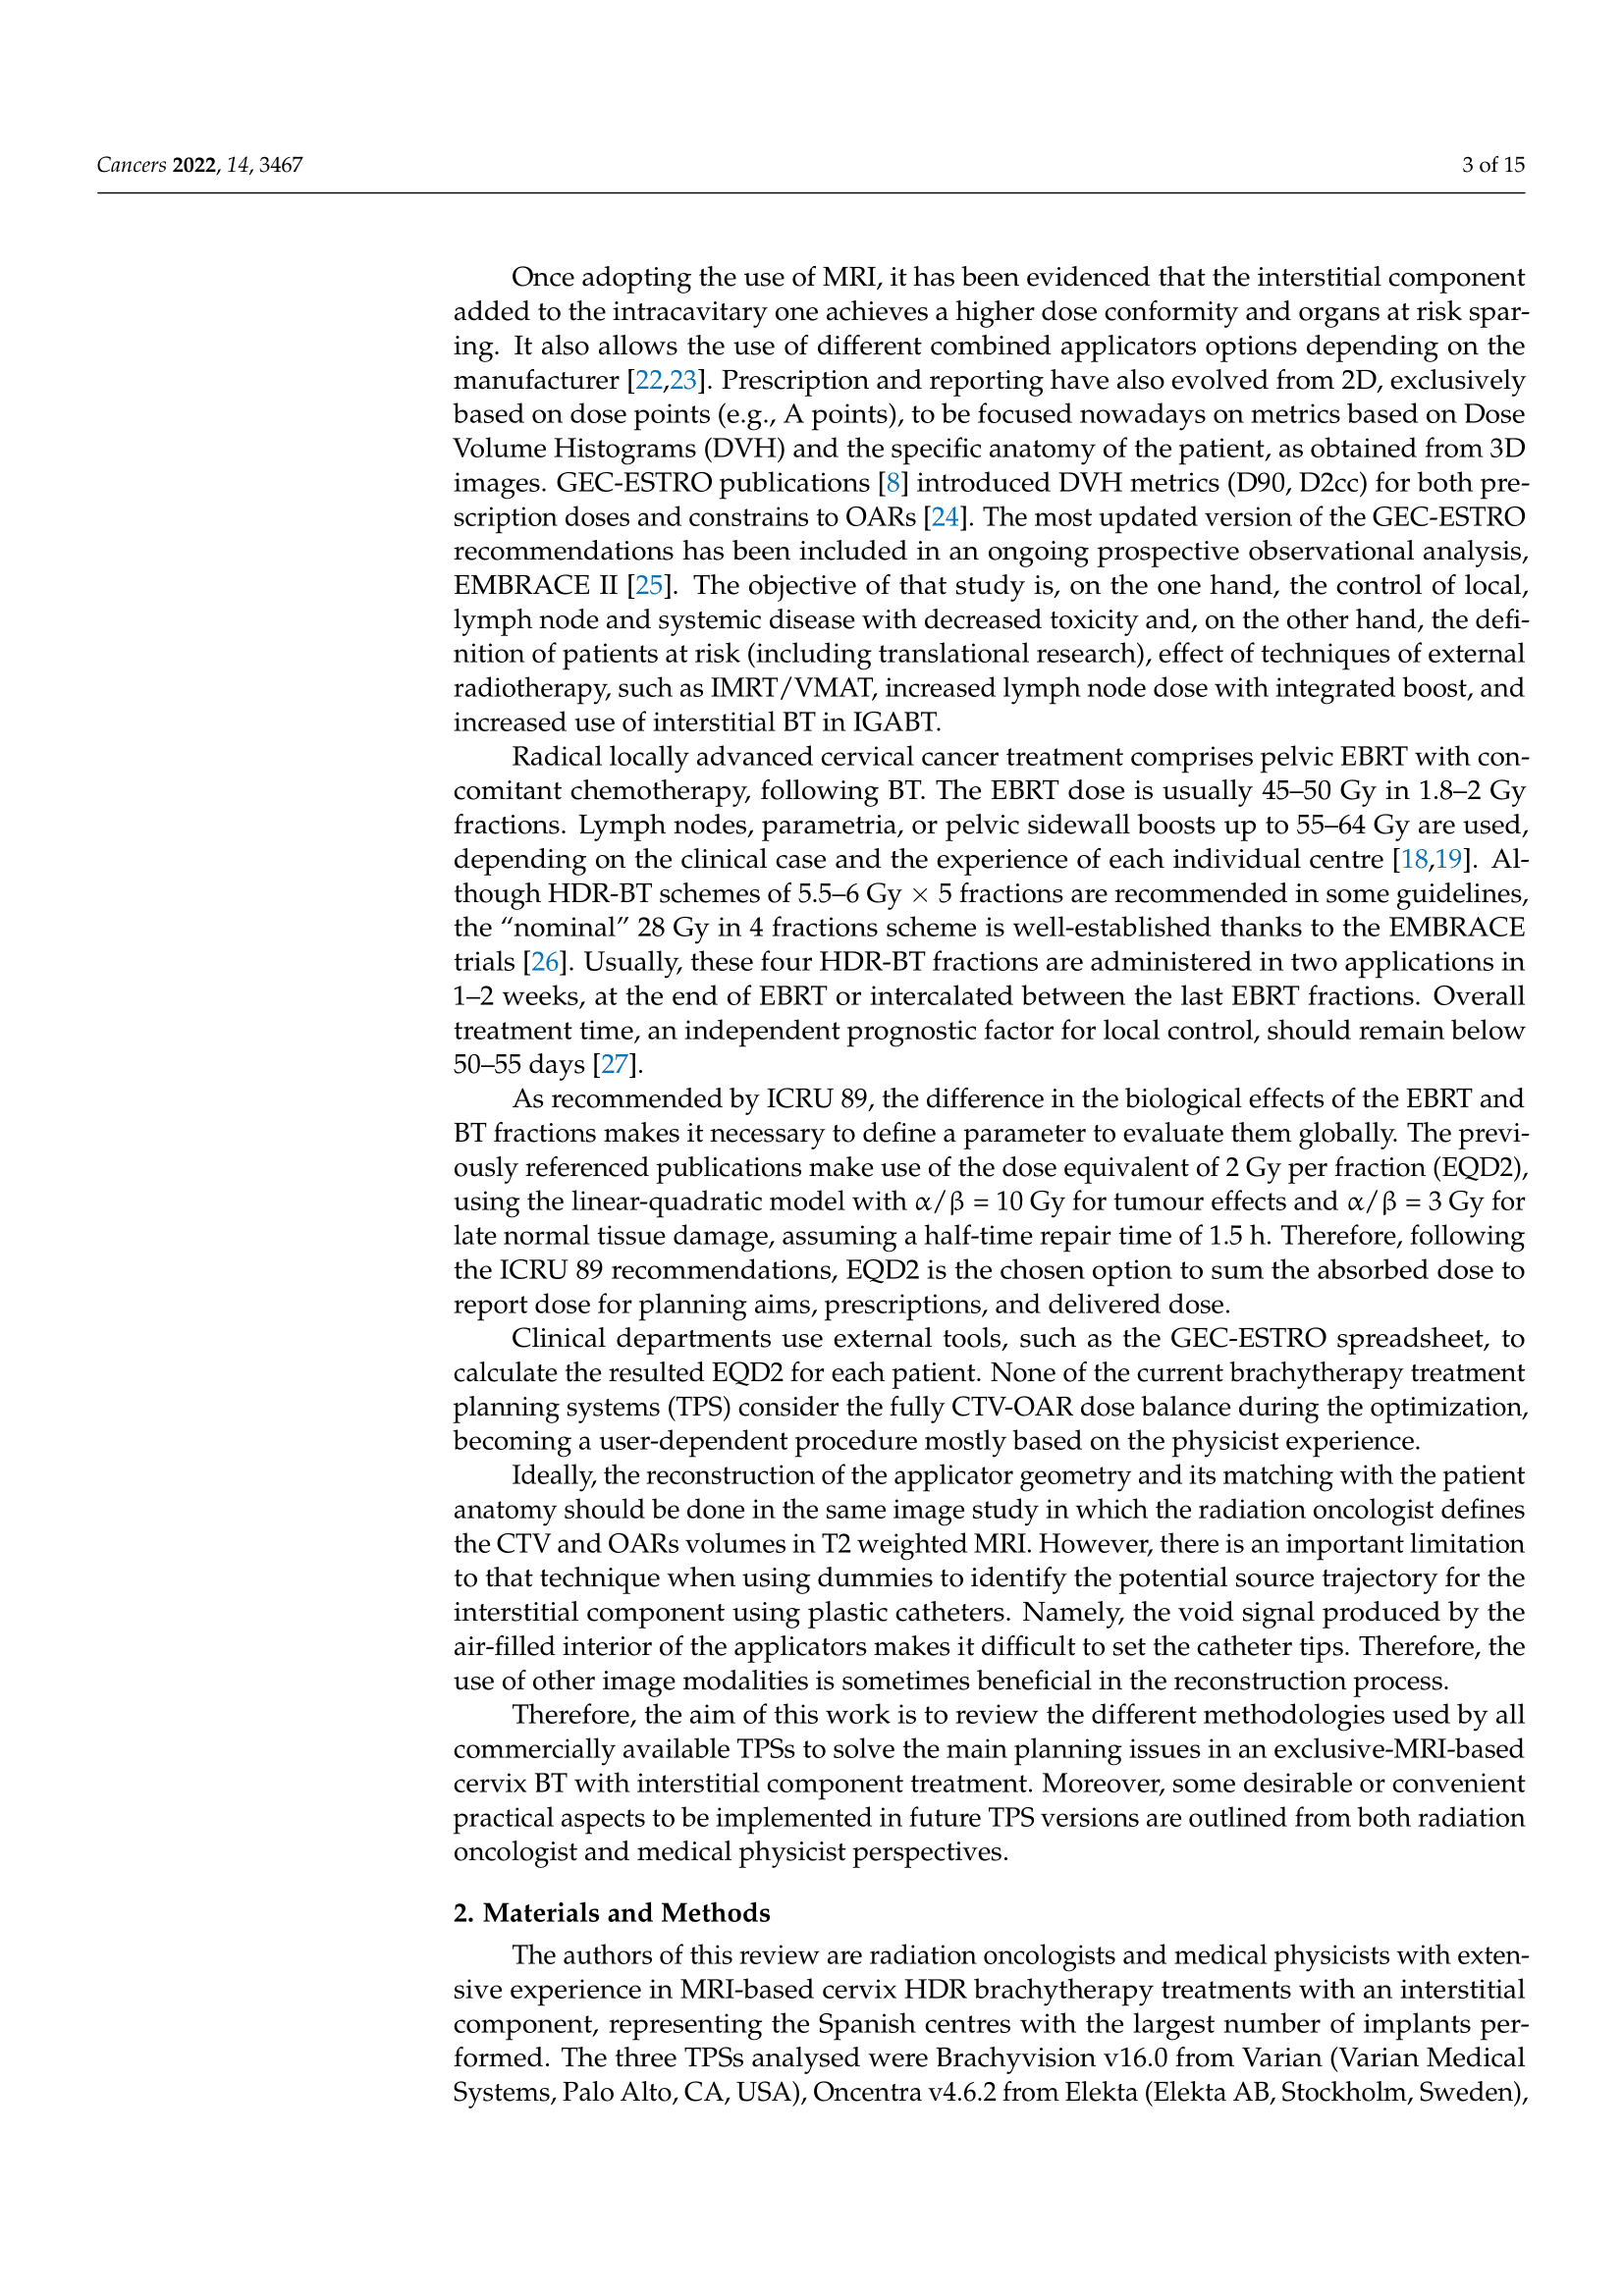
\includegraphics{articulos/cancers/cancers-03.png}
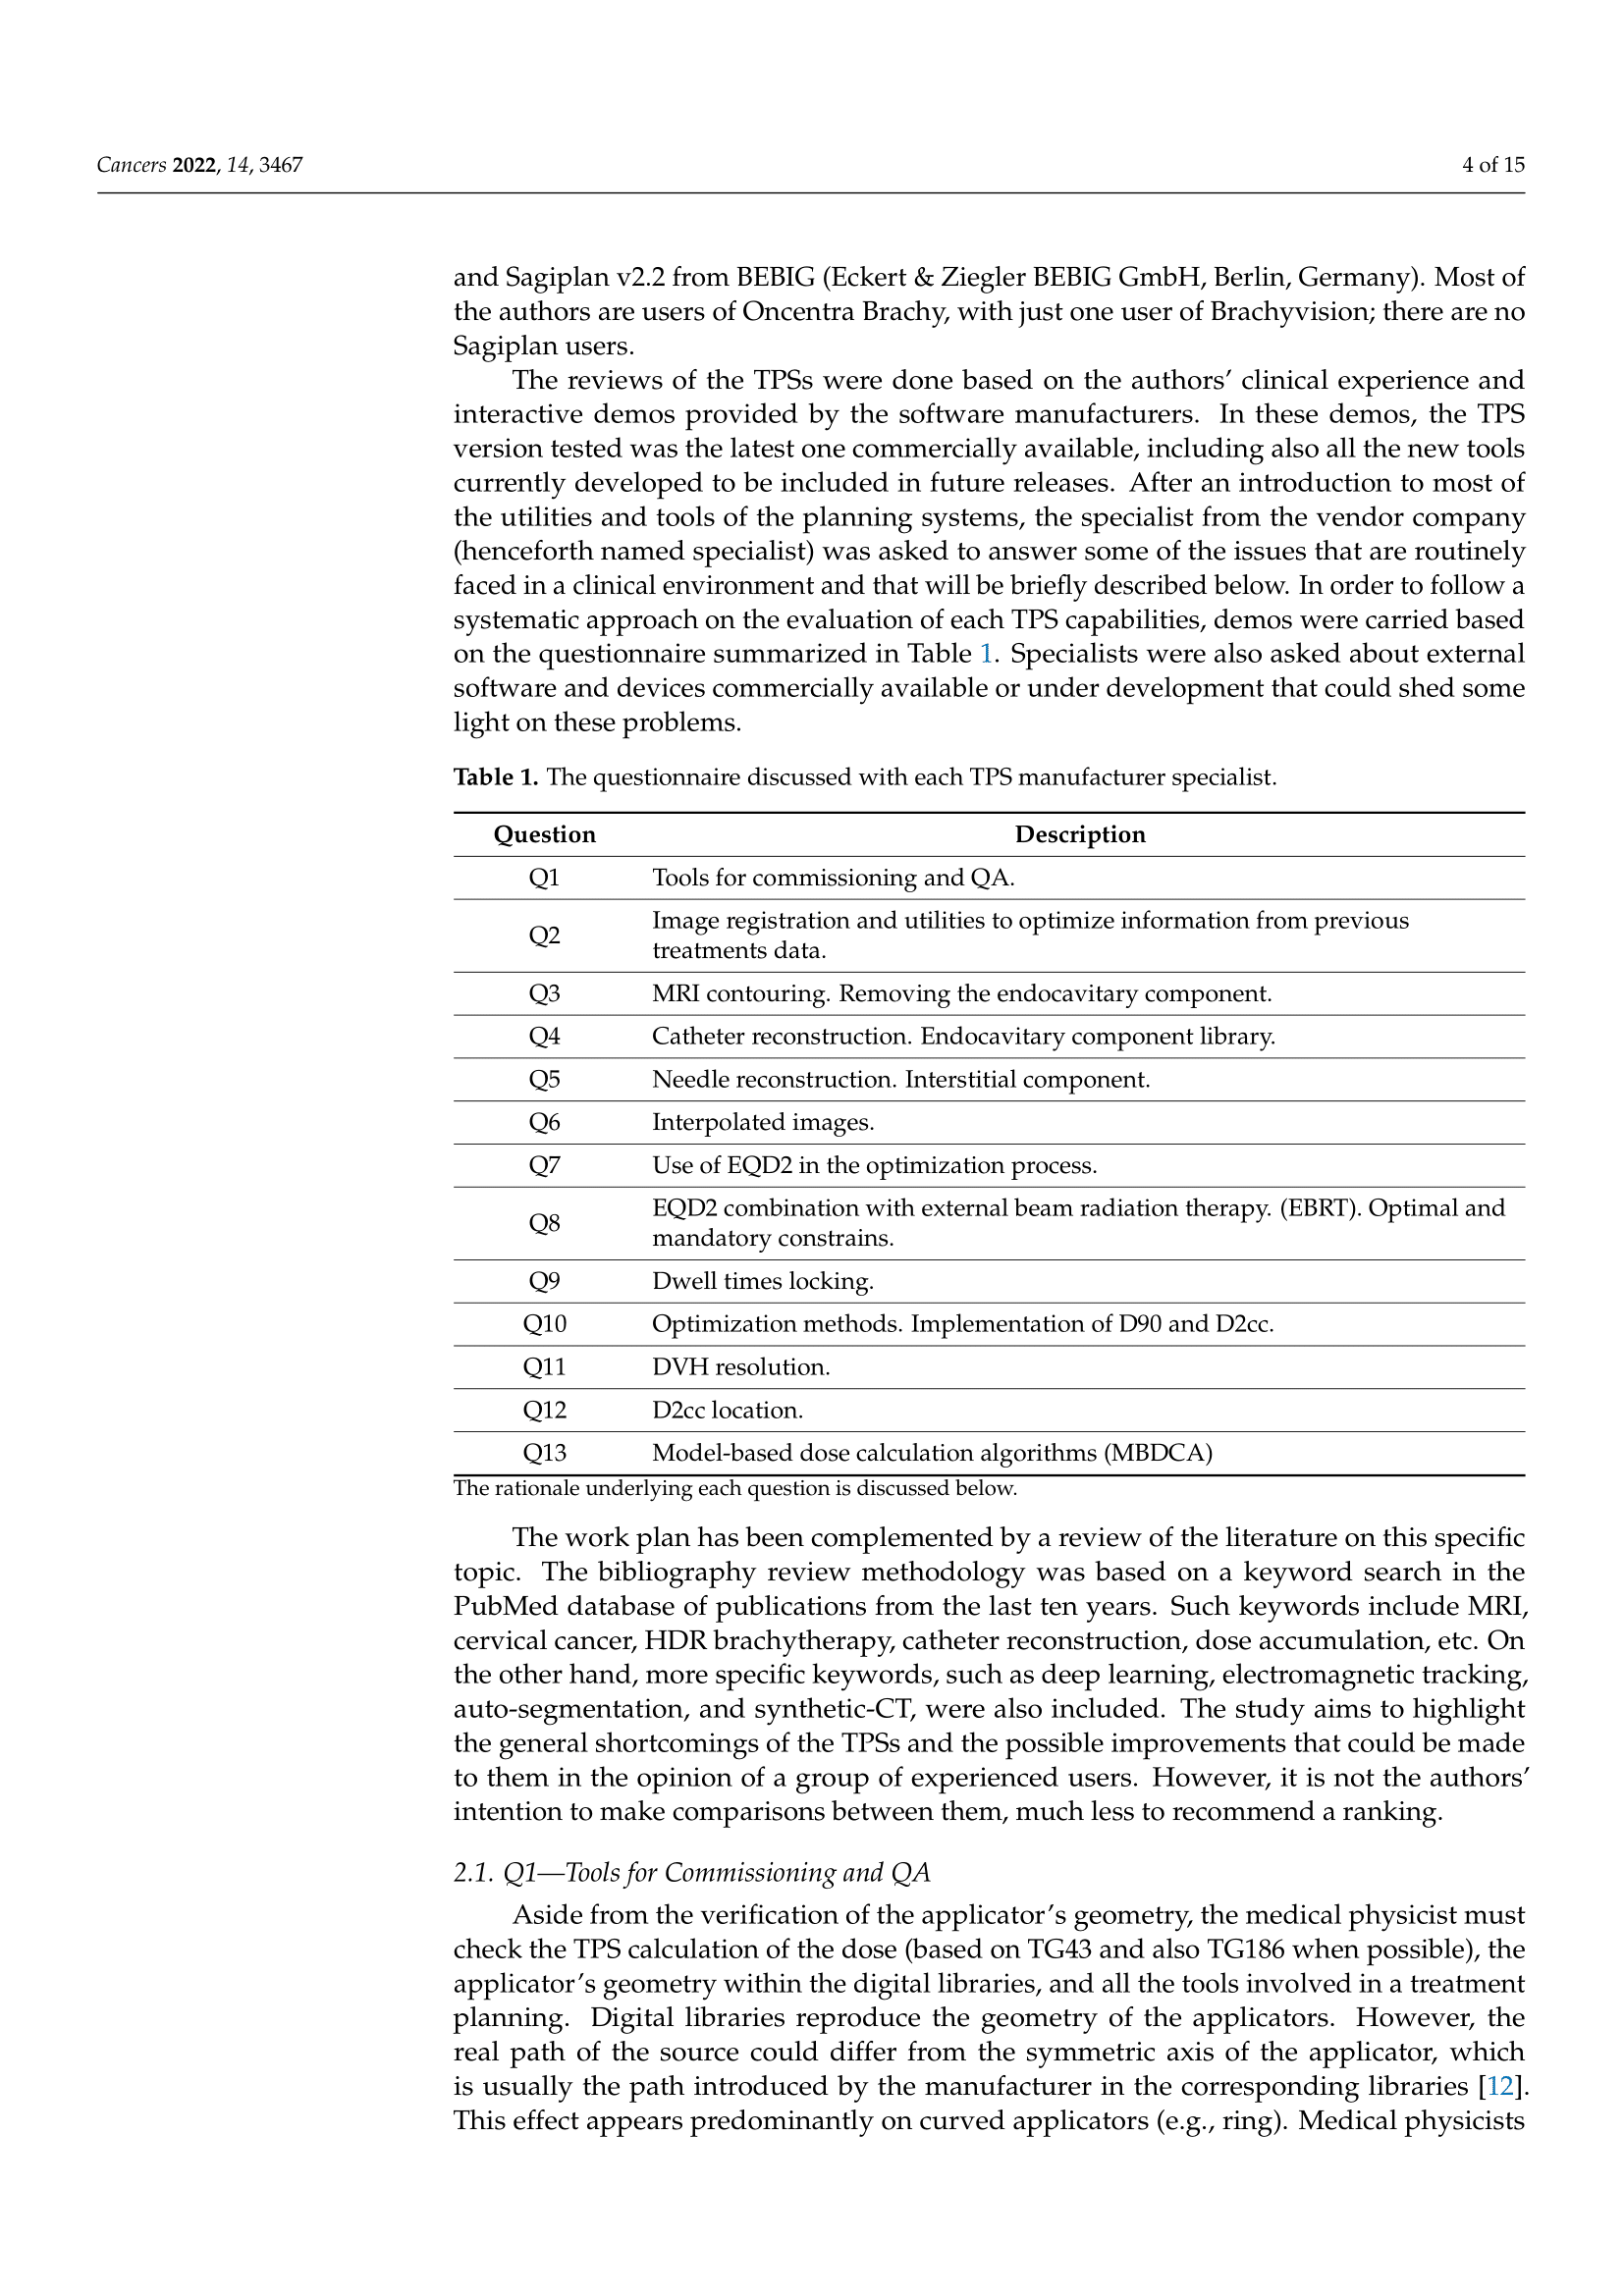
\includegraphics{articulos/cancers/cancers-04.png}
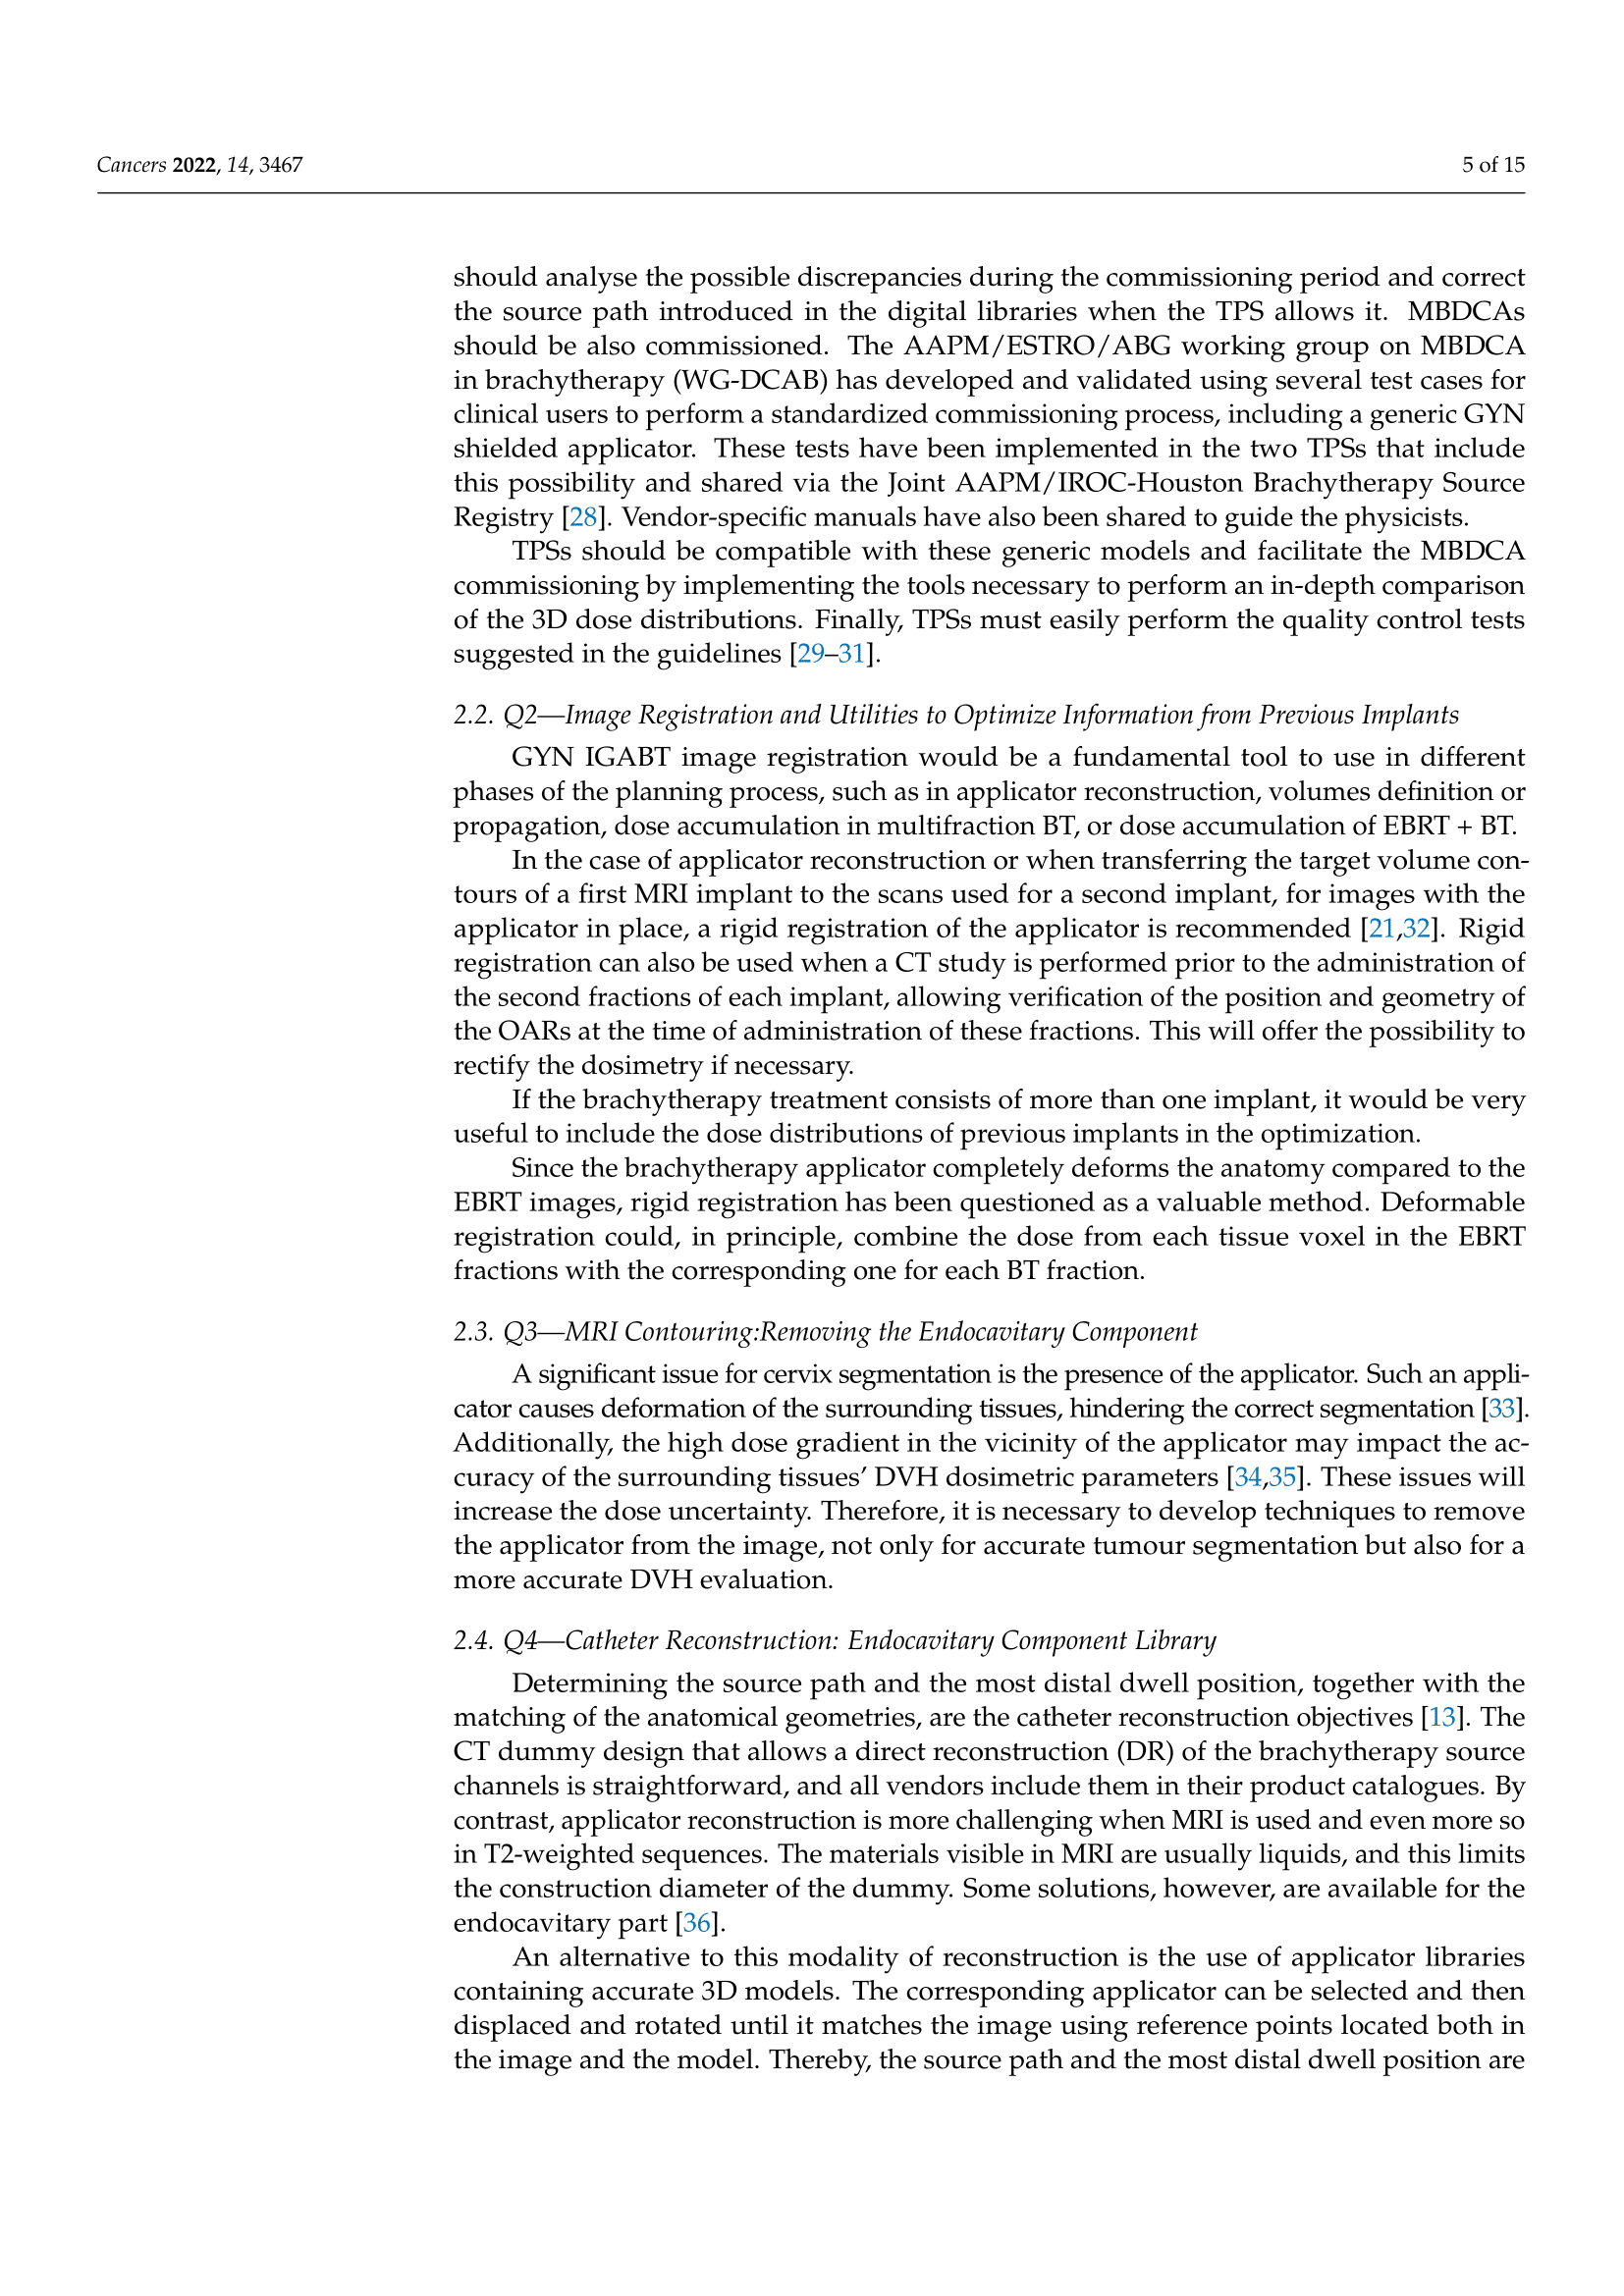
\includegraphics{articulos/cancers/cancers-05.png}
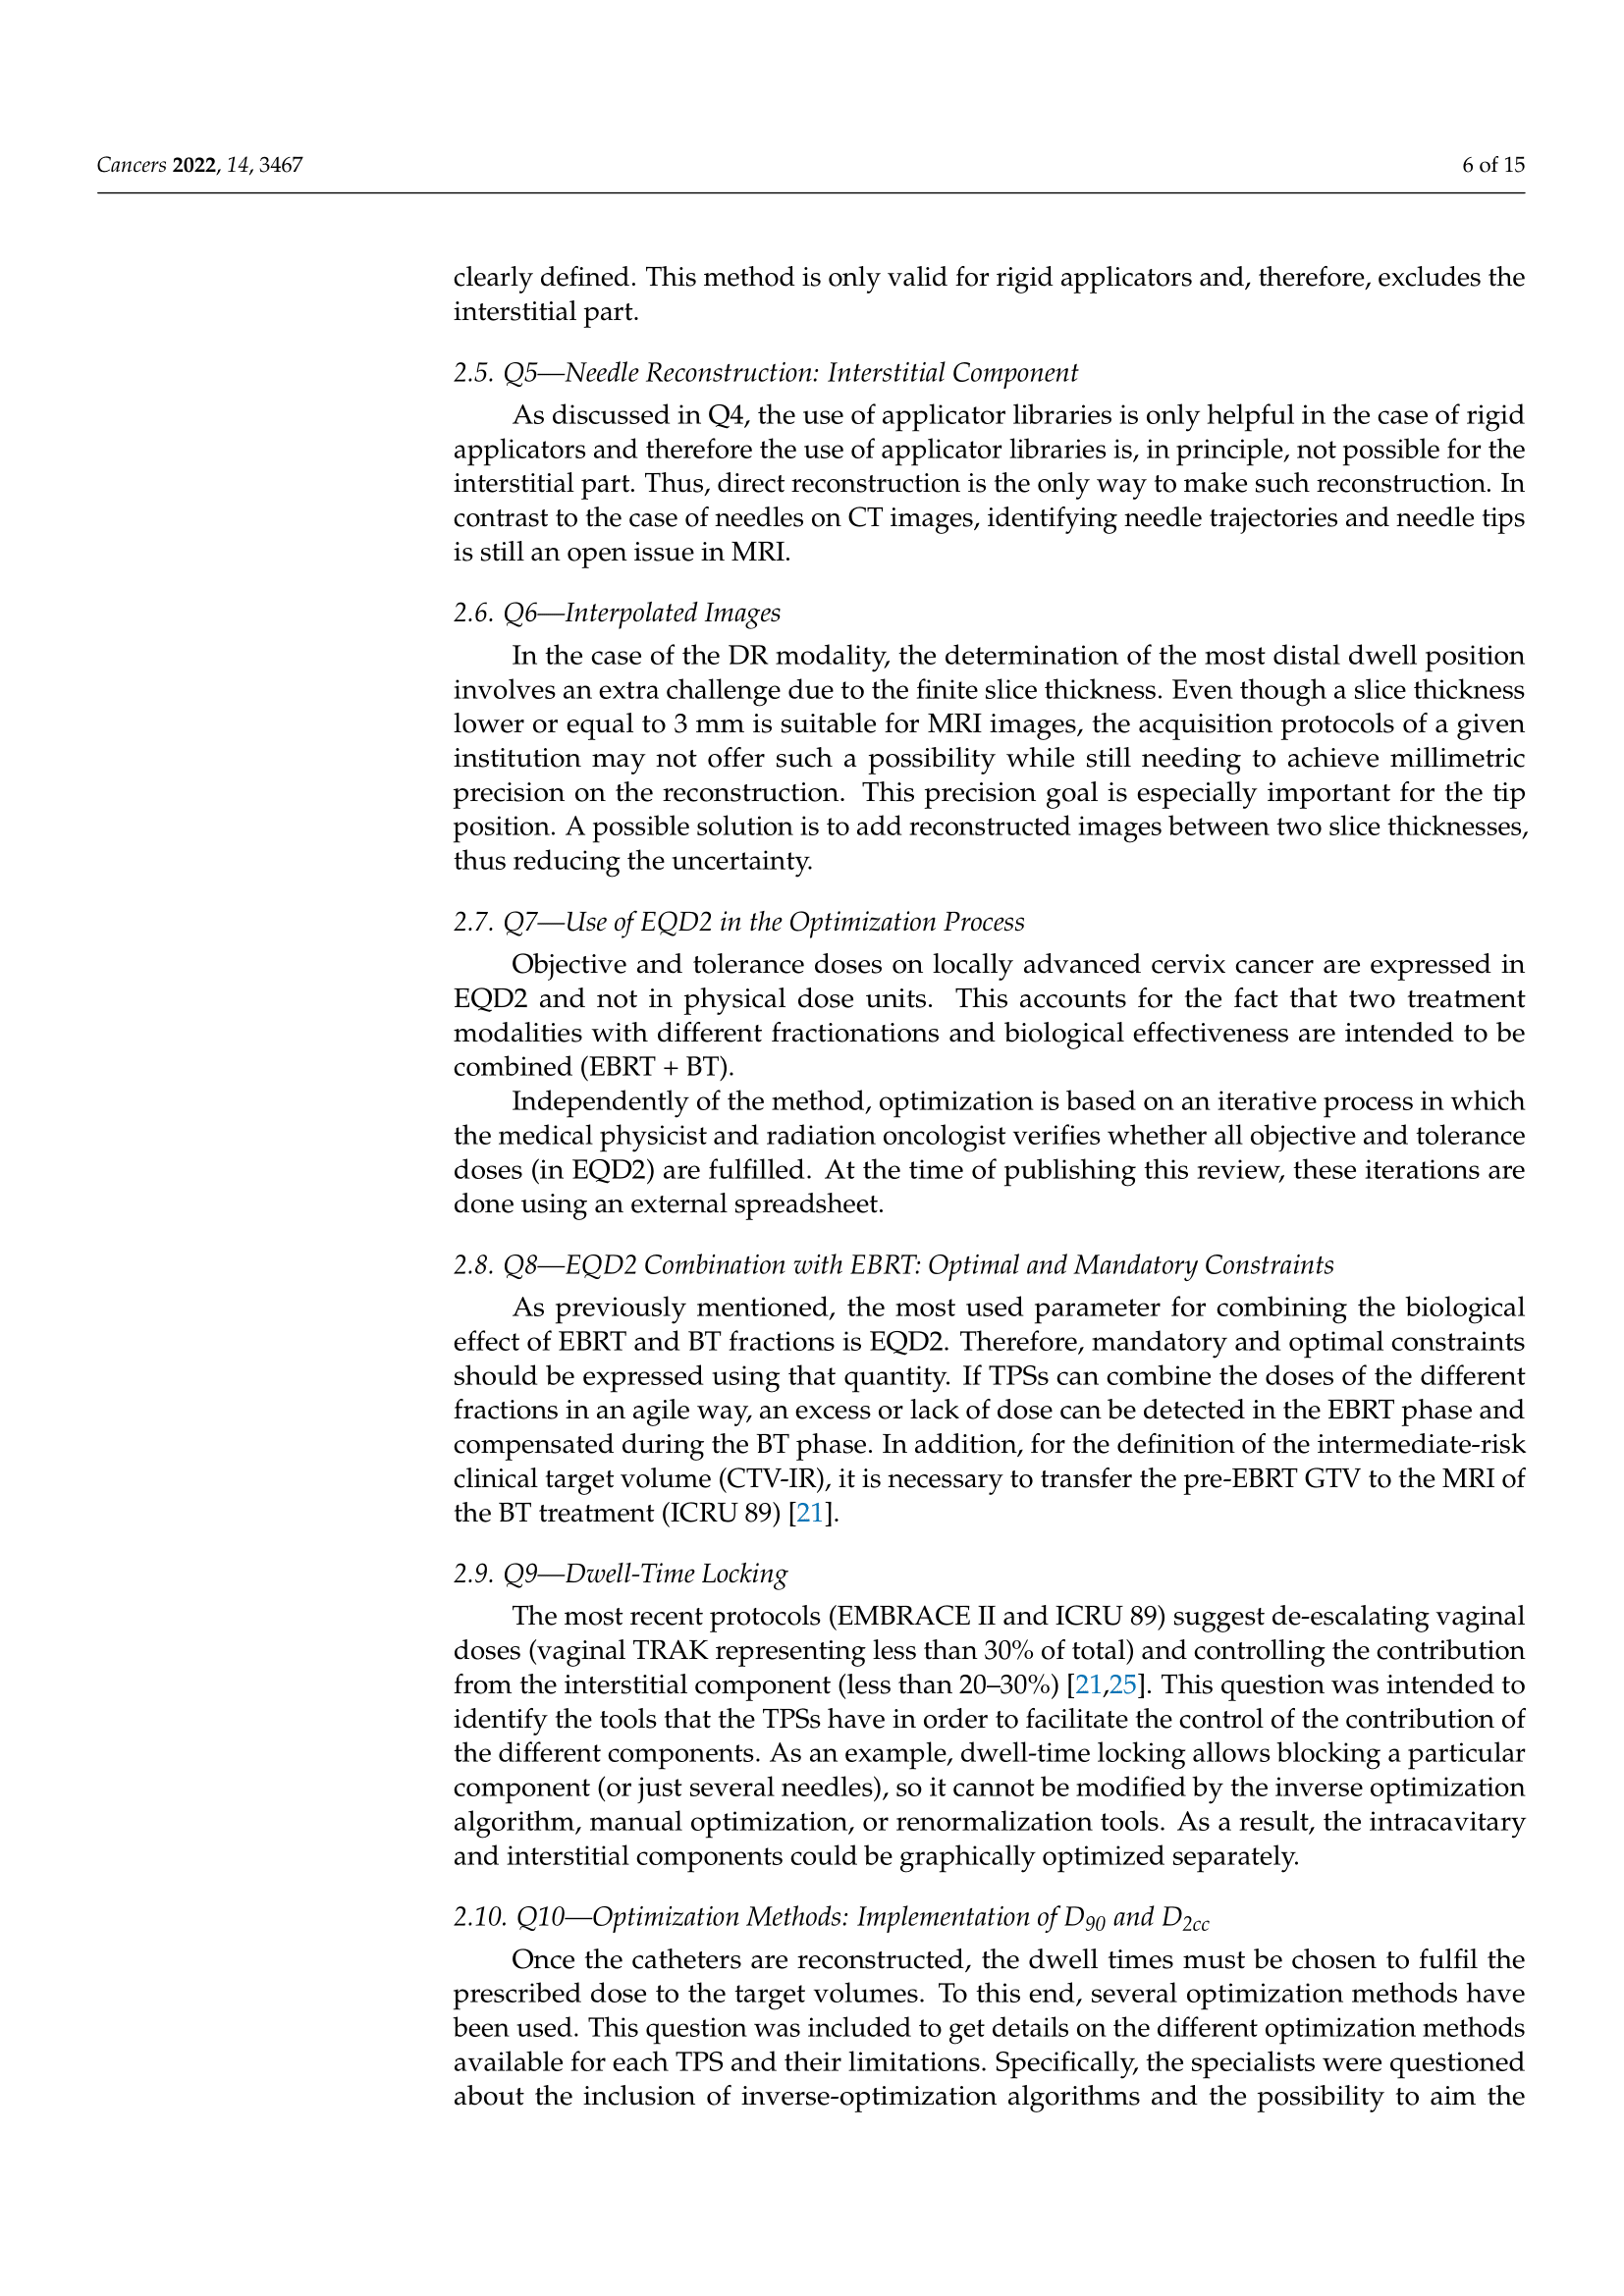
\includegraphics{articulos/cancers/cancers-06.png}
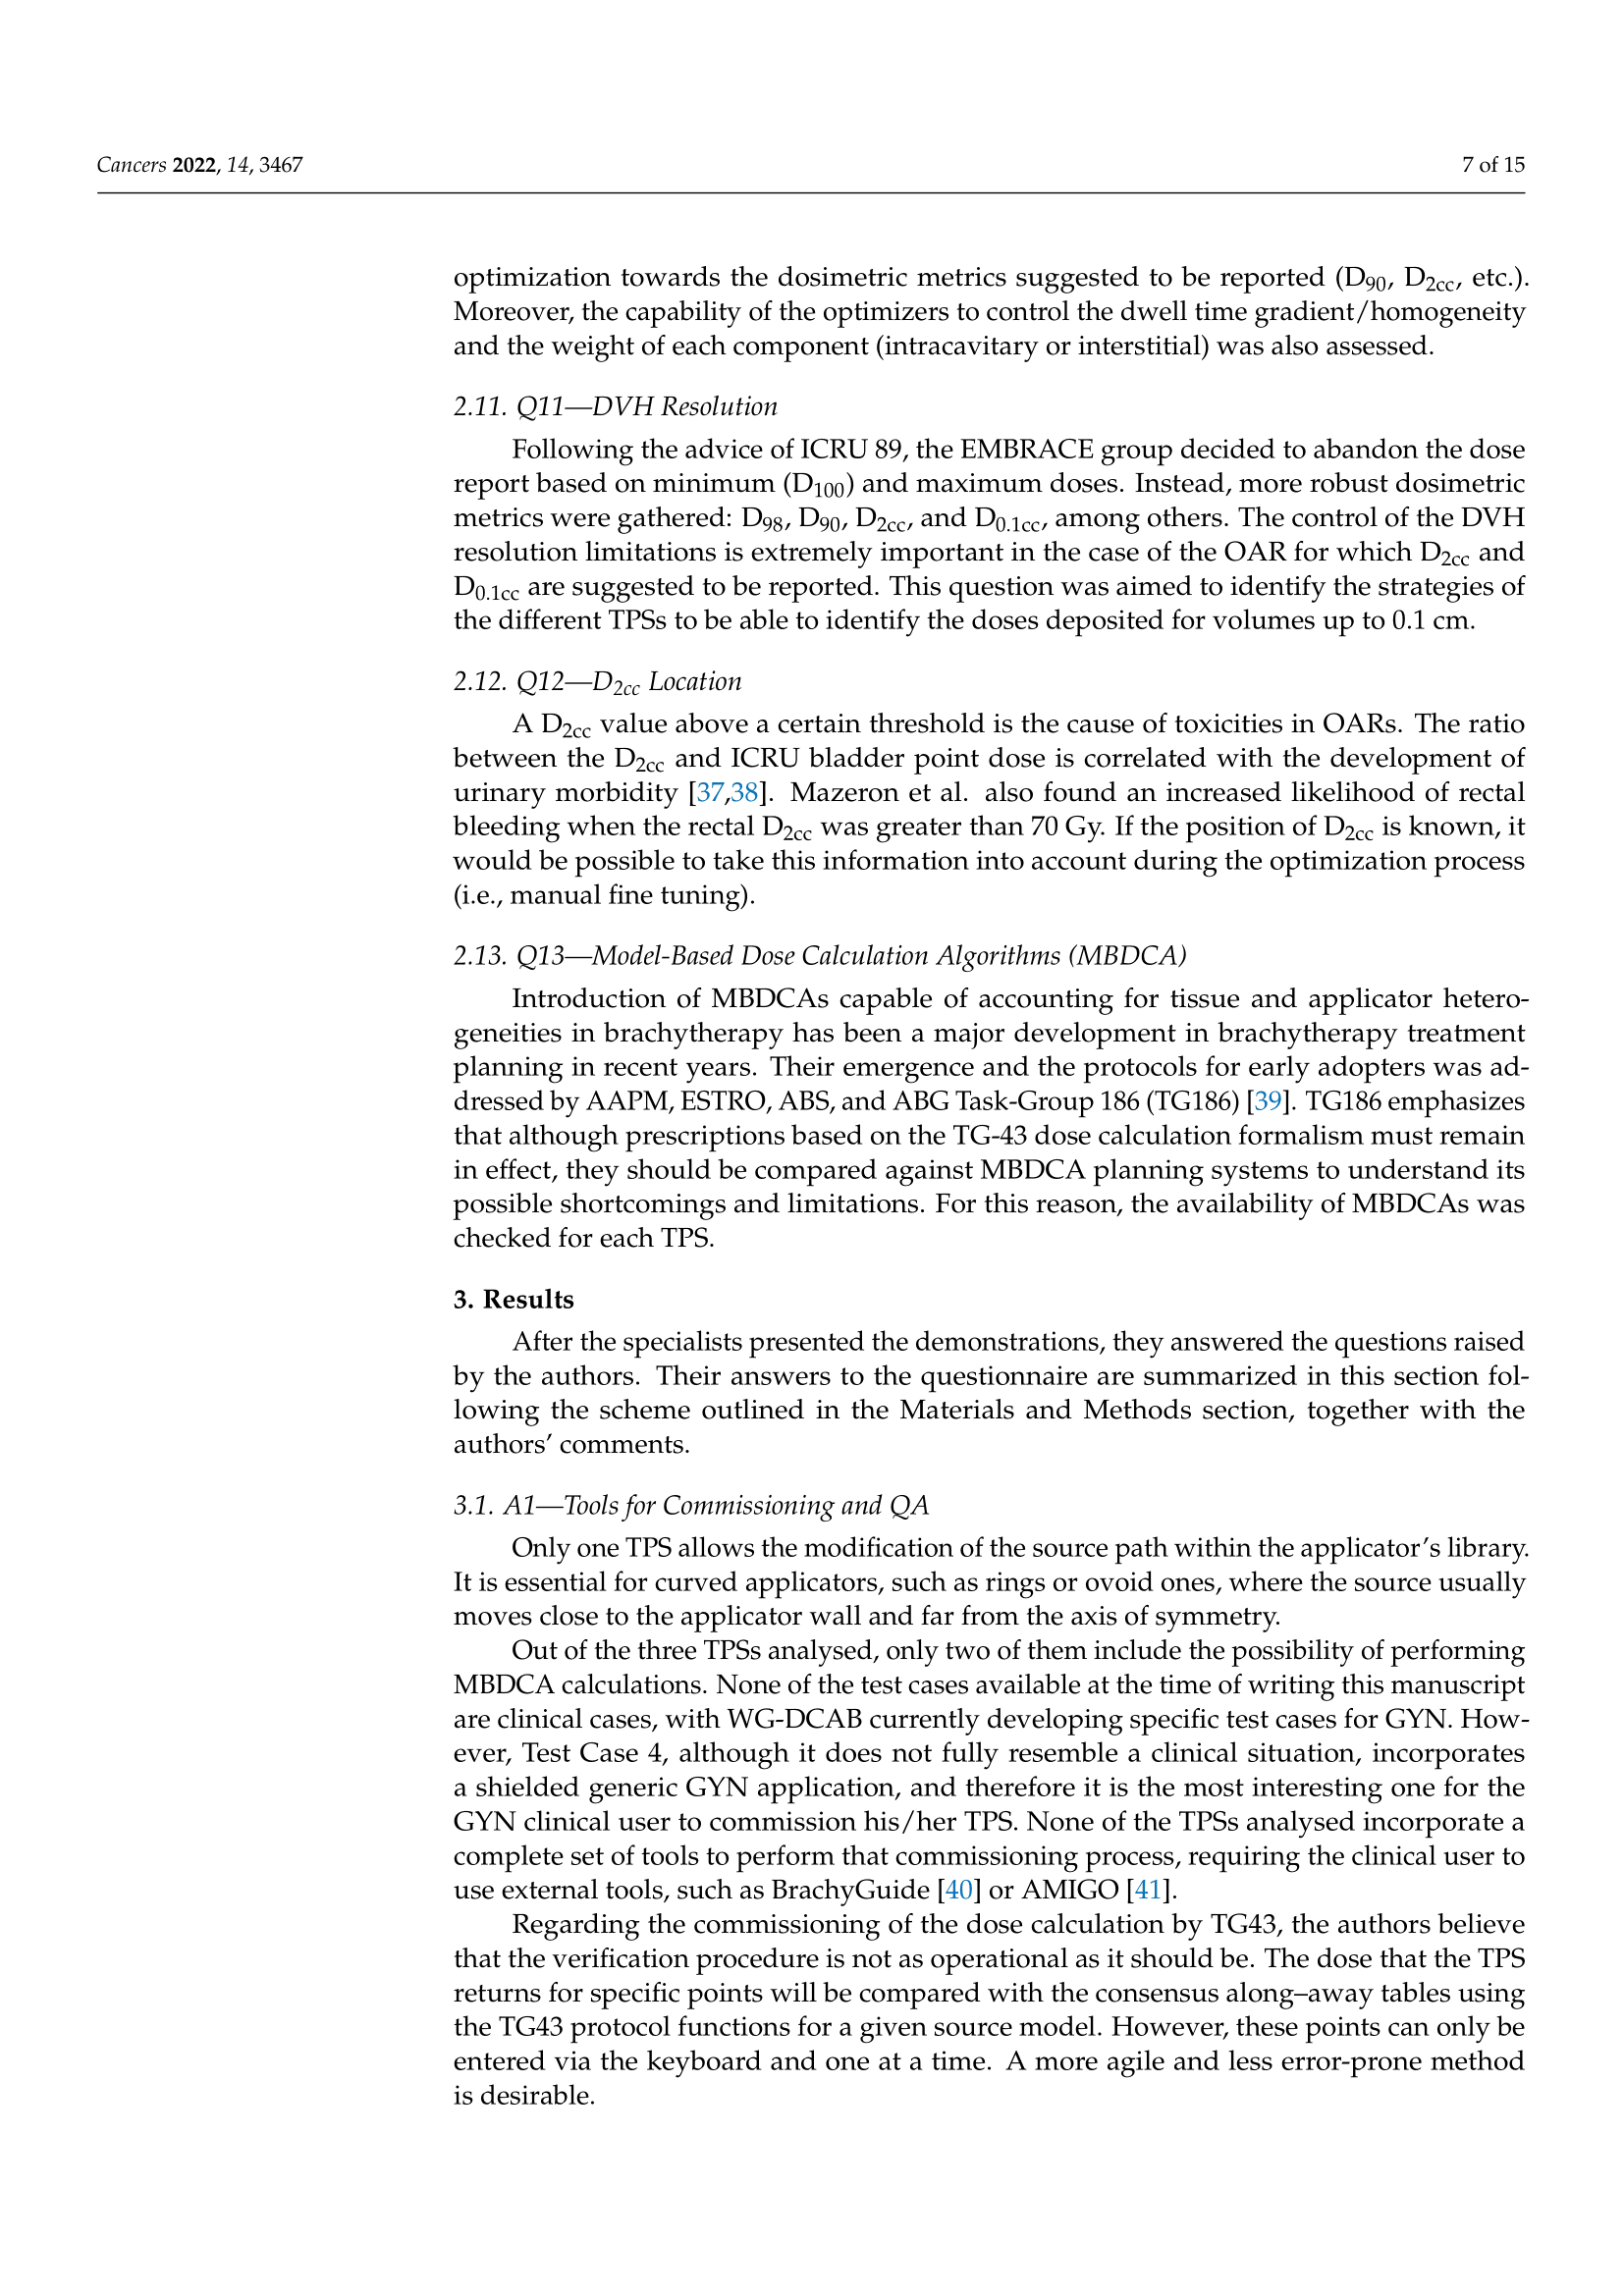
\includegraphics{articulos/cancers/cancers-07.png}
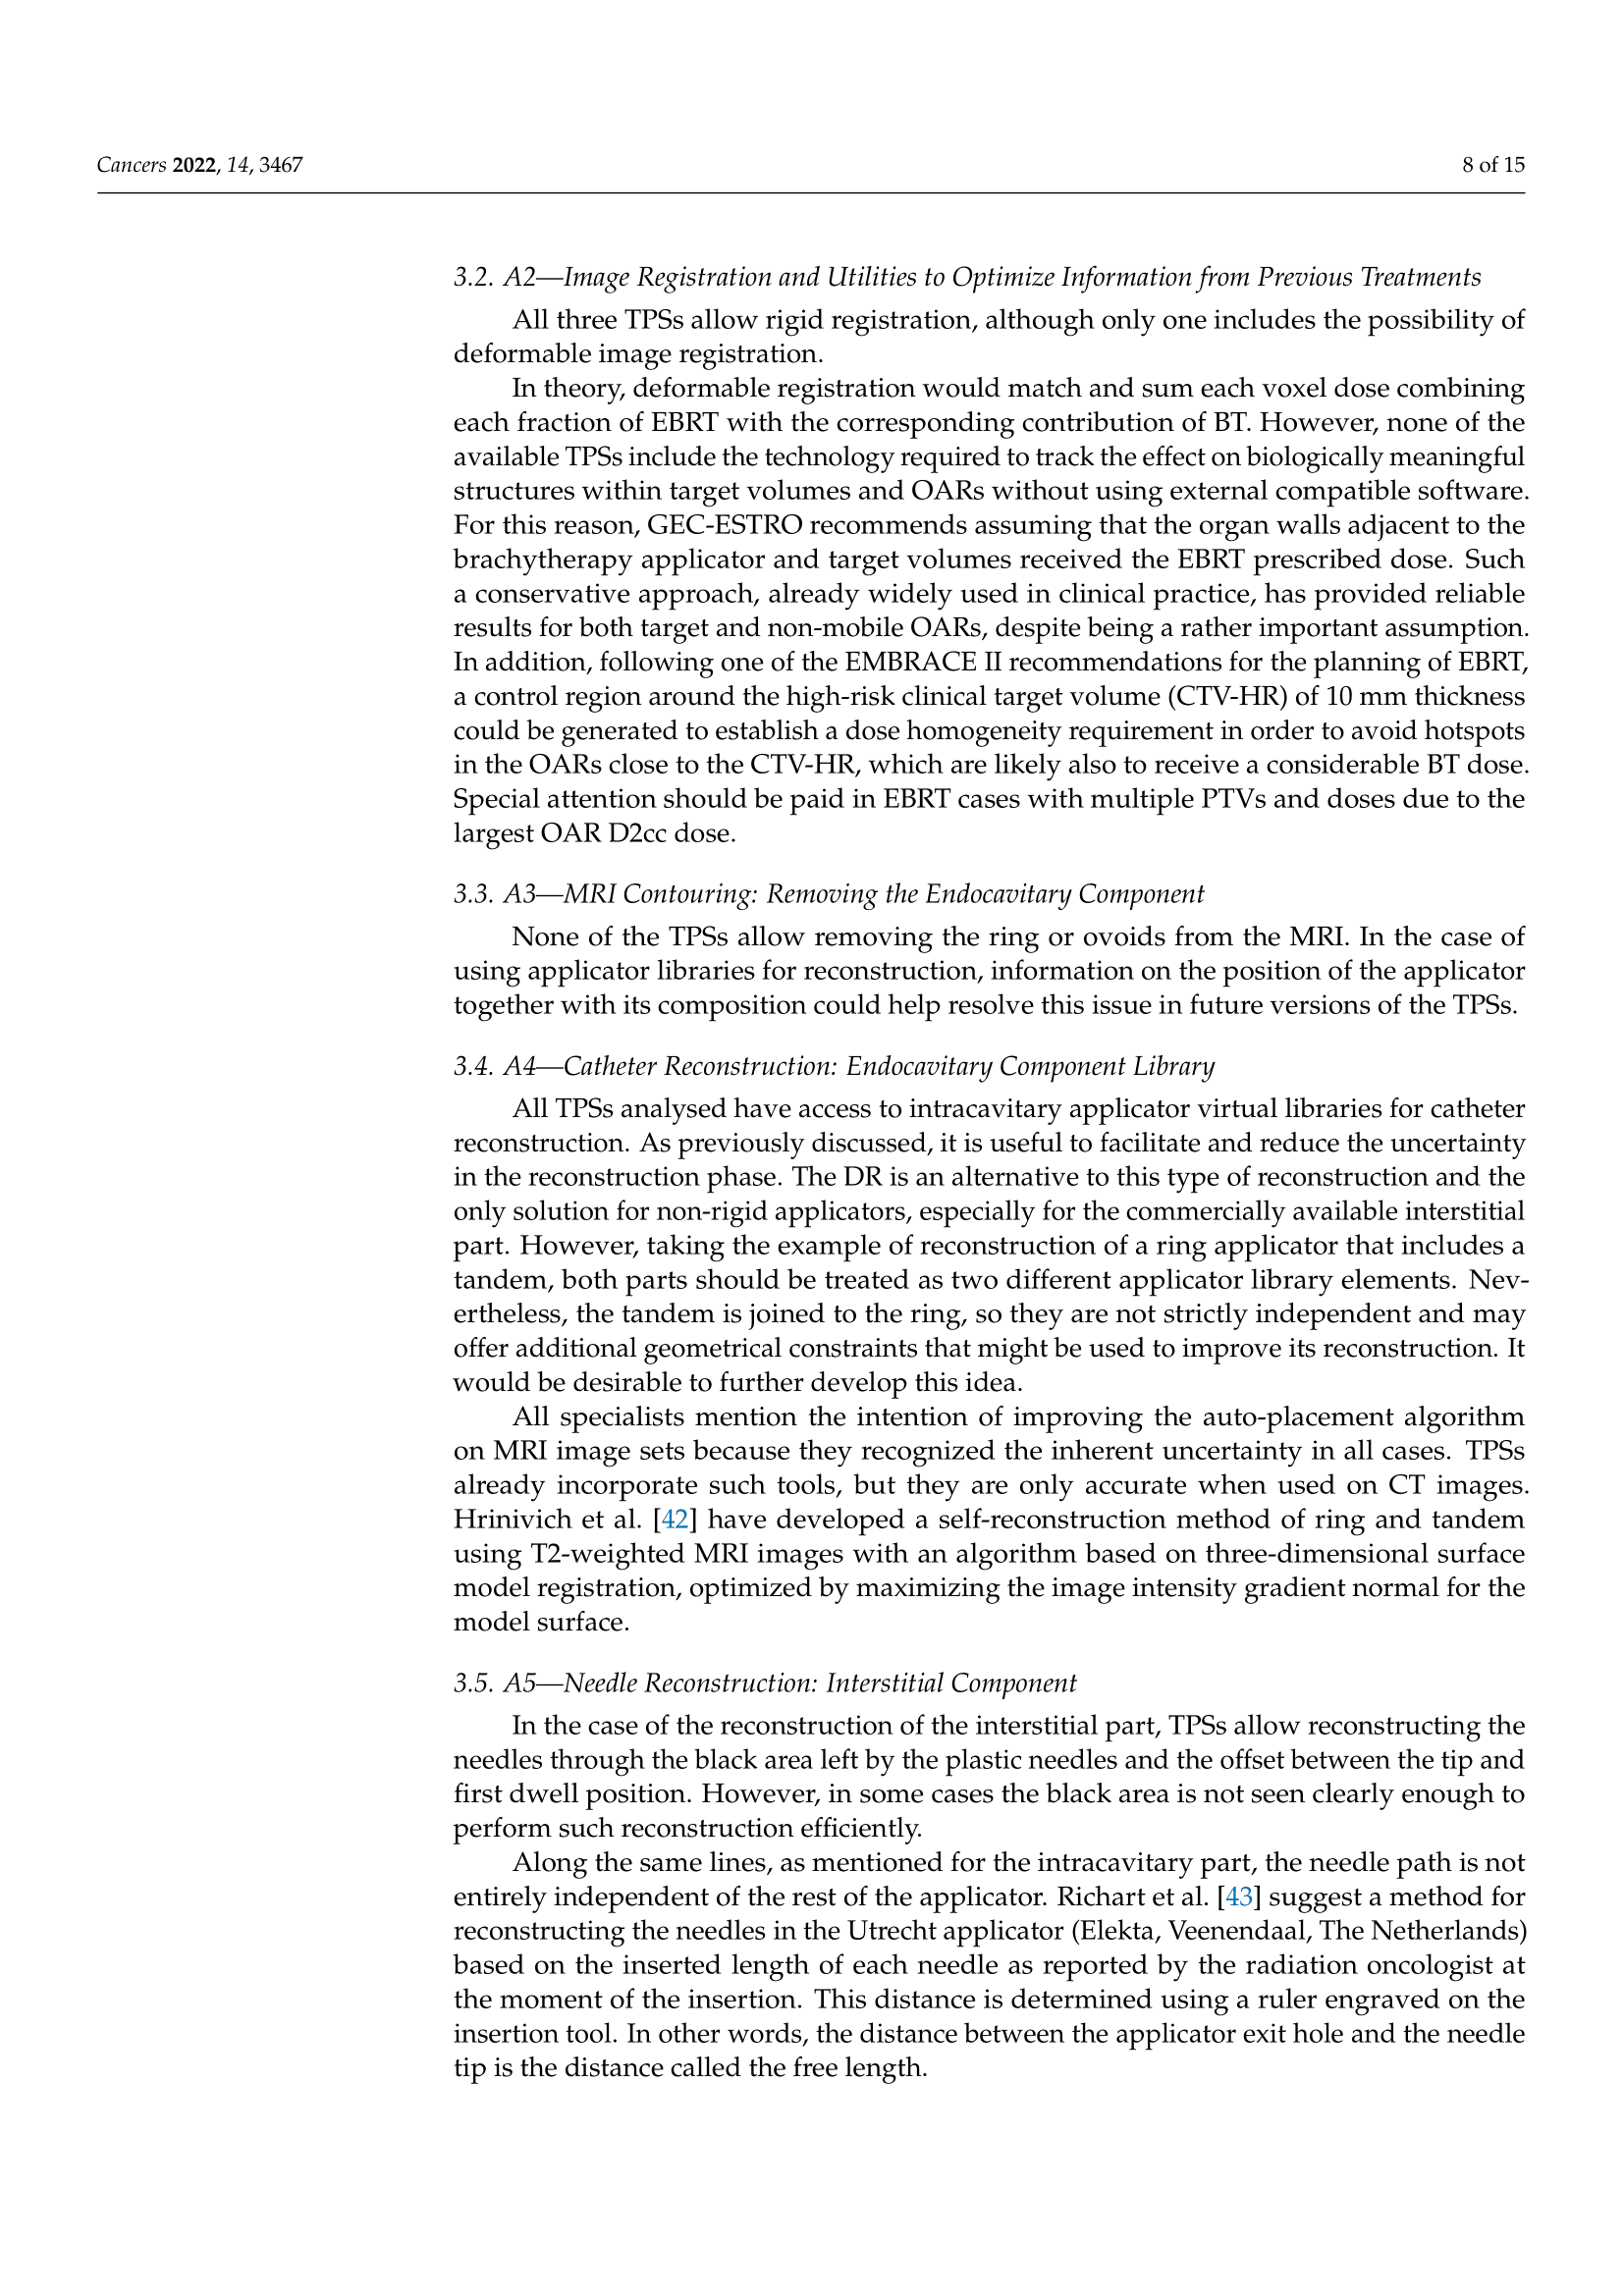
\includegraphics{articulos/cancers/cancers-08.png}
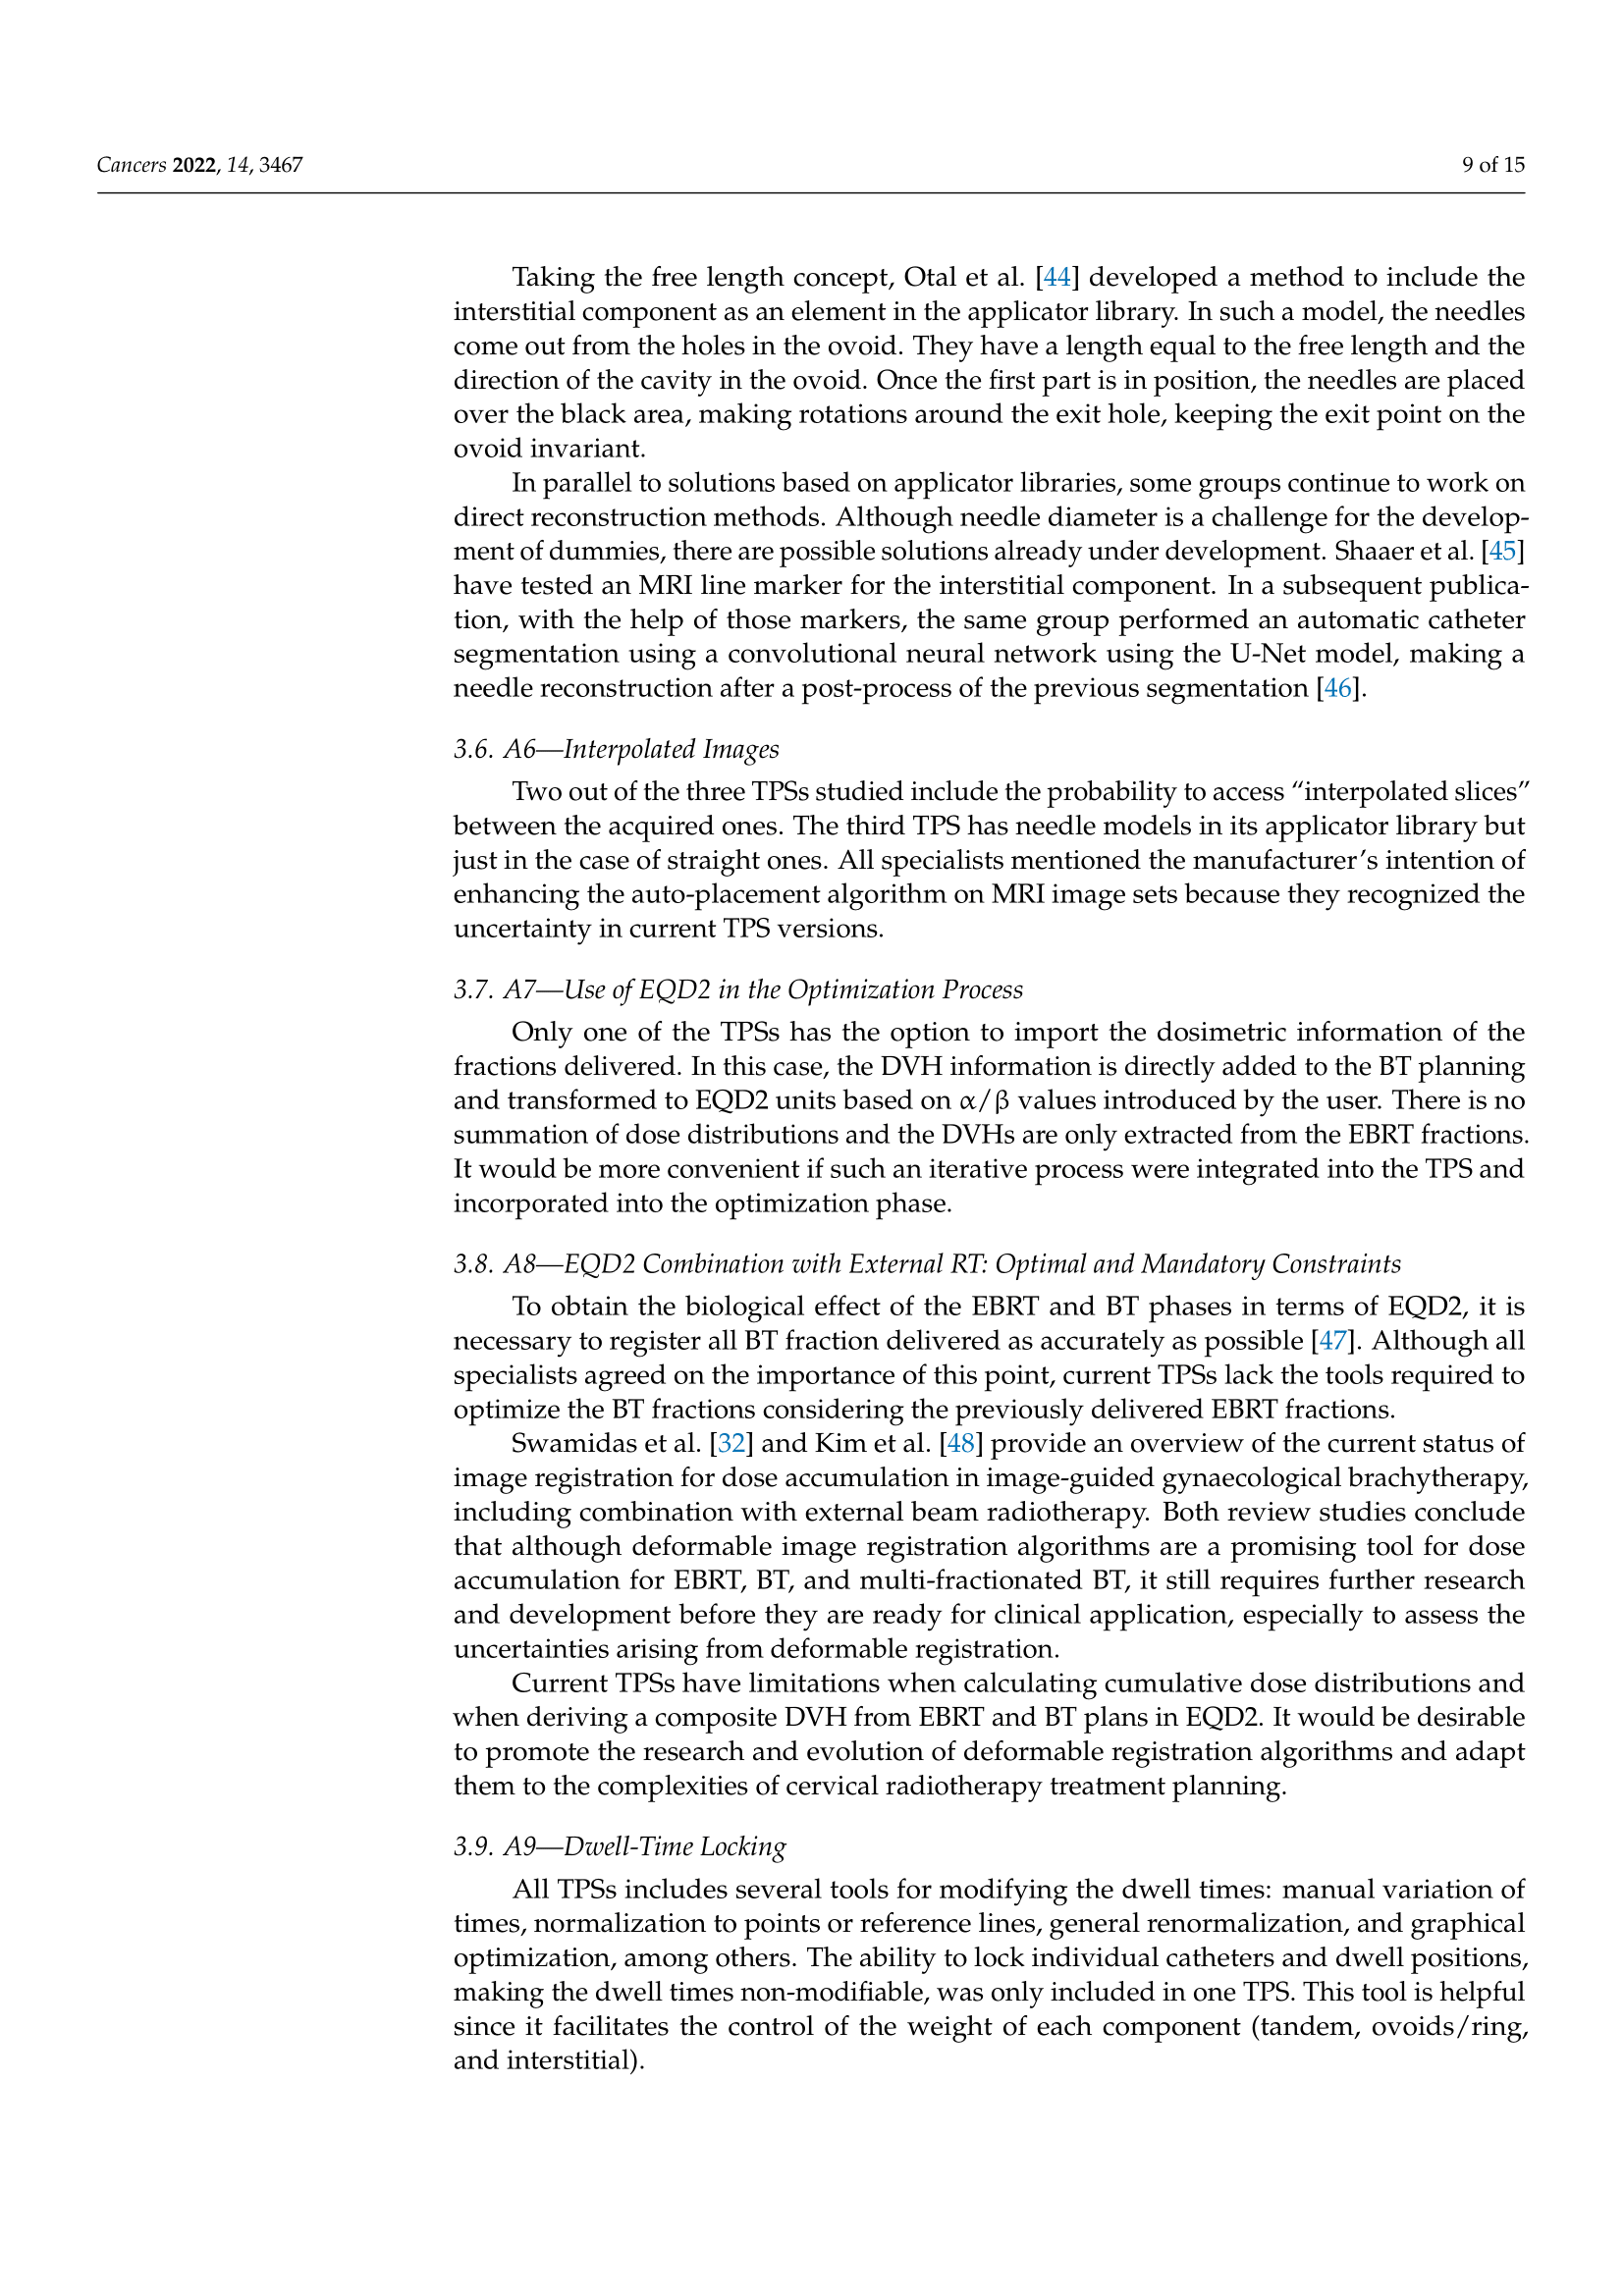
\includegraphics{articulos/cancers/cancers-09.png}
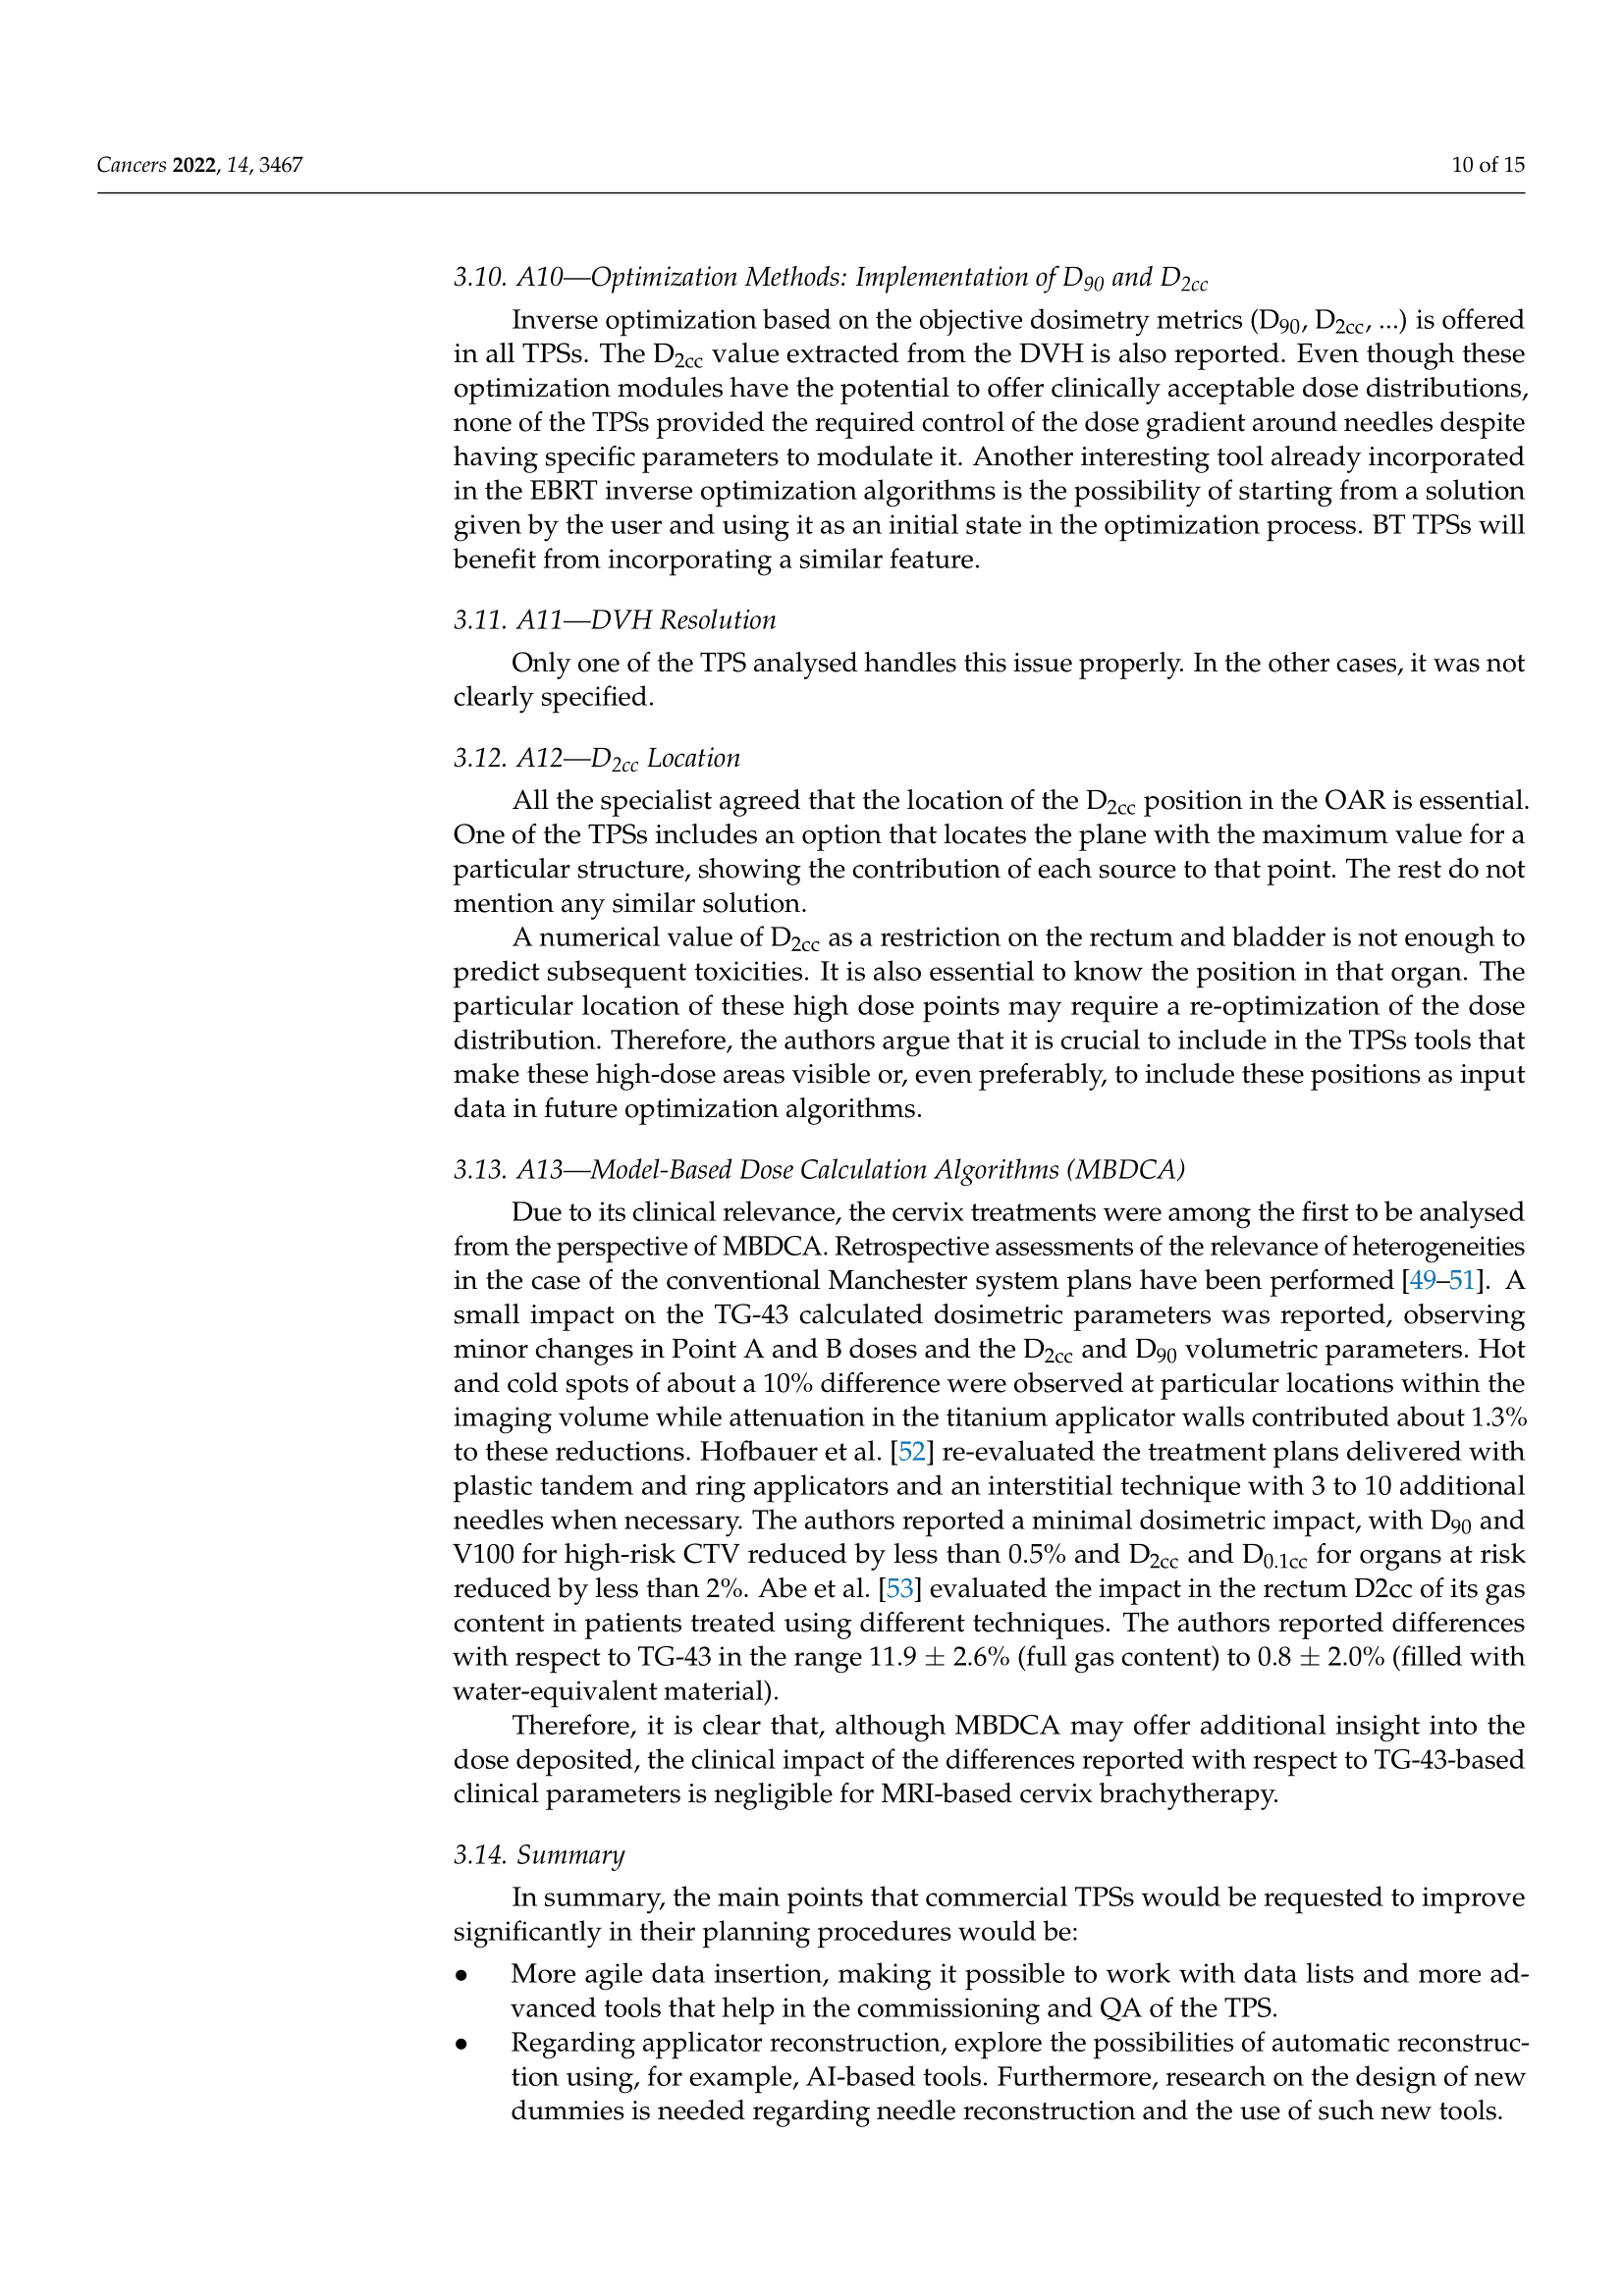
\includegraphics{articulos/cancers/cancers-10.png}
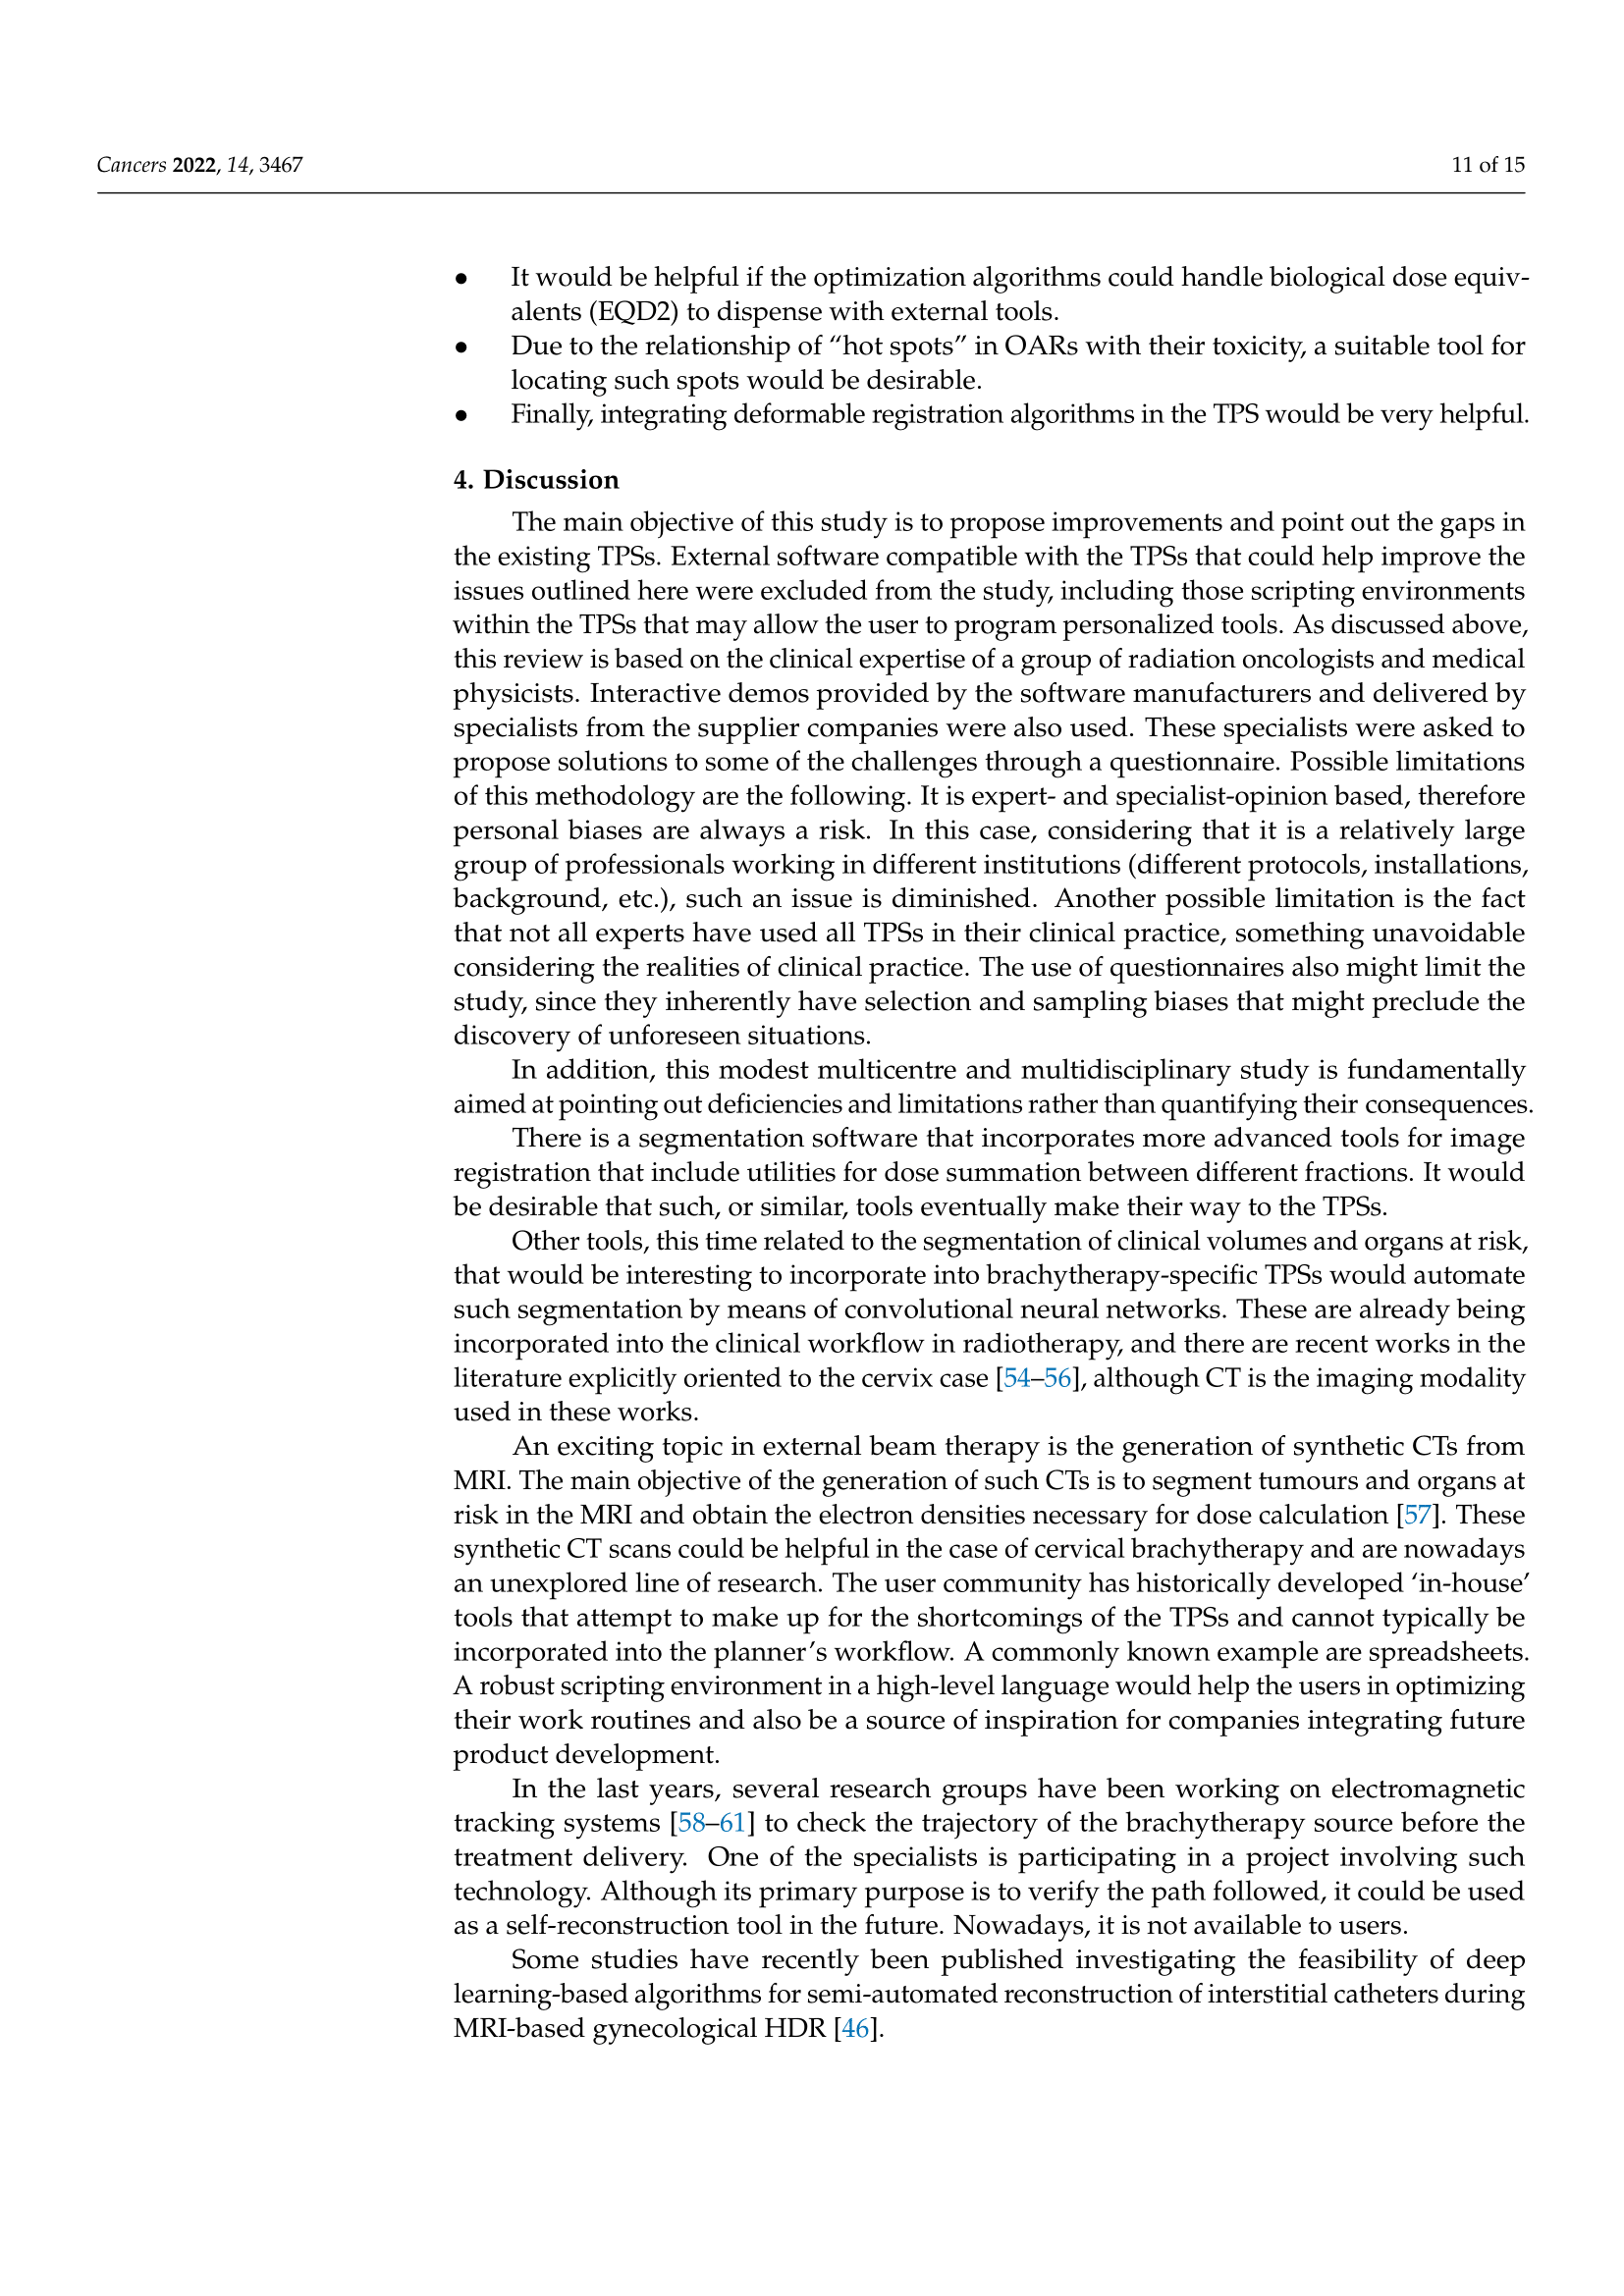
\includegraphics{articulos/cancers/cancers-11.png}
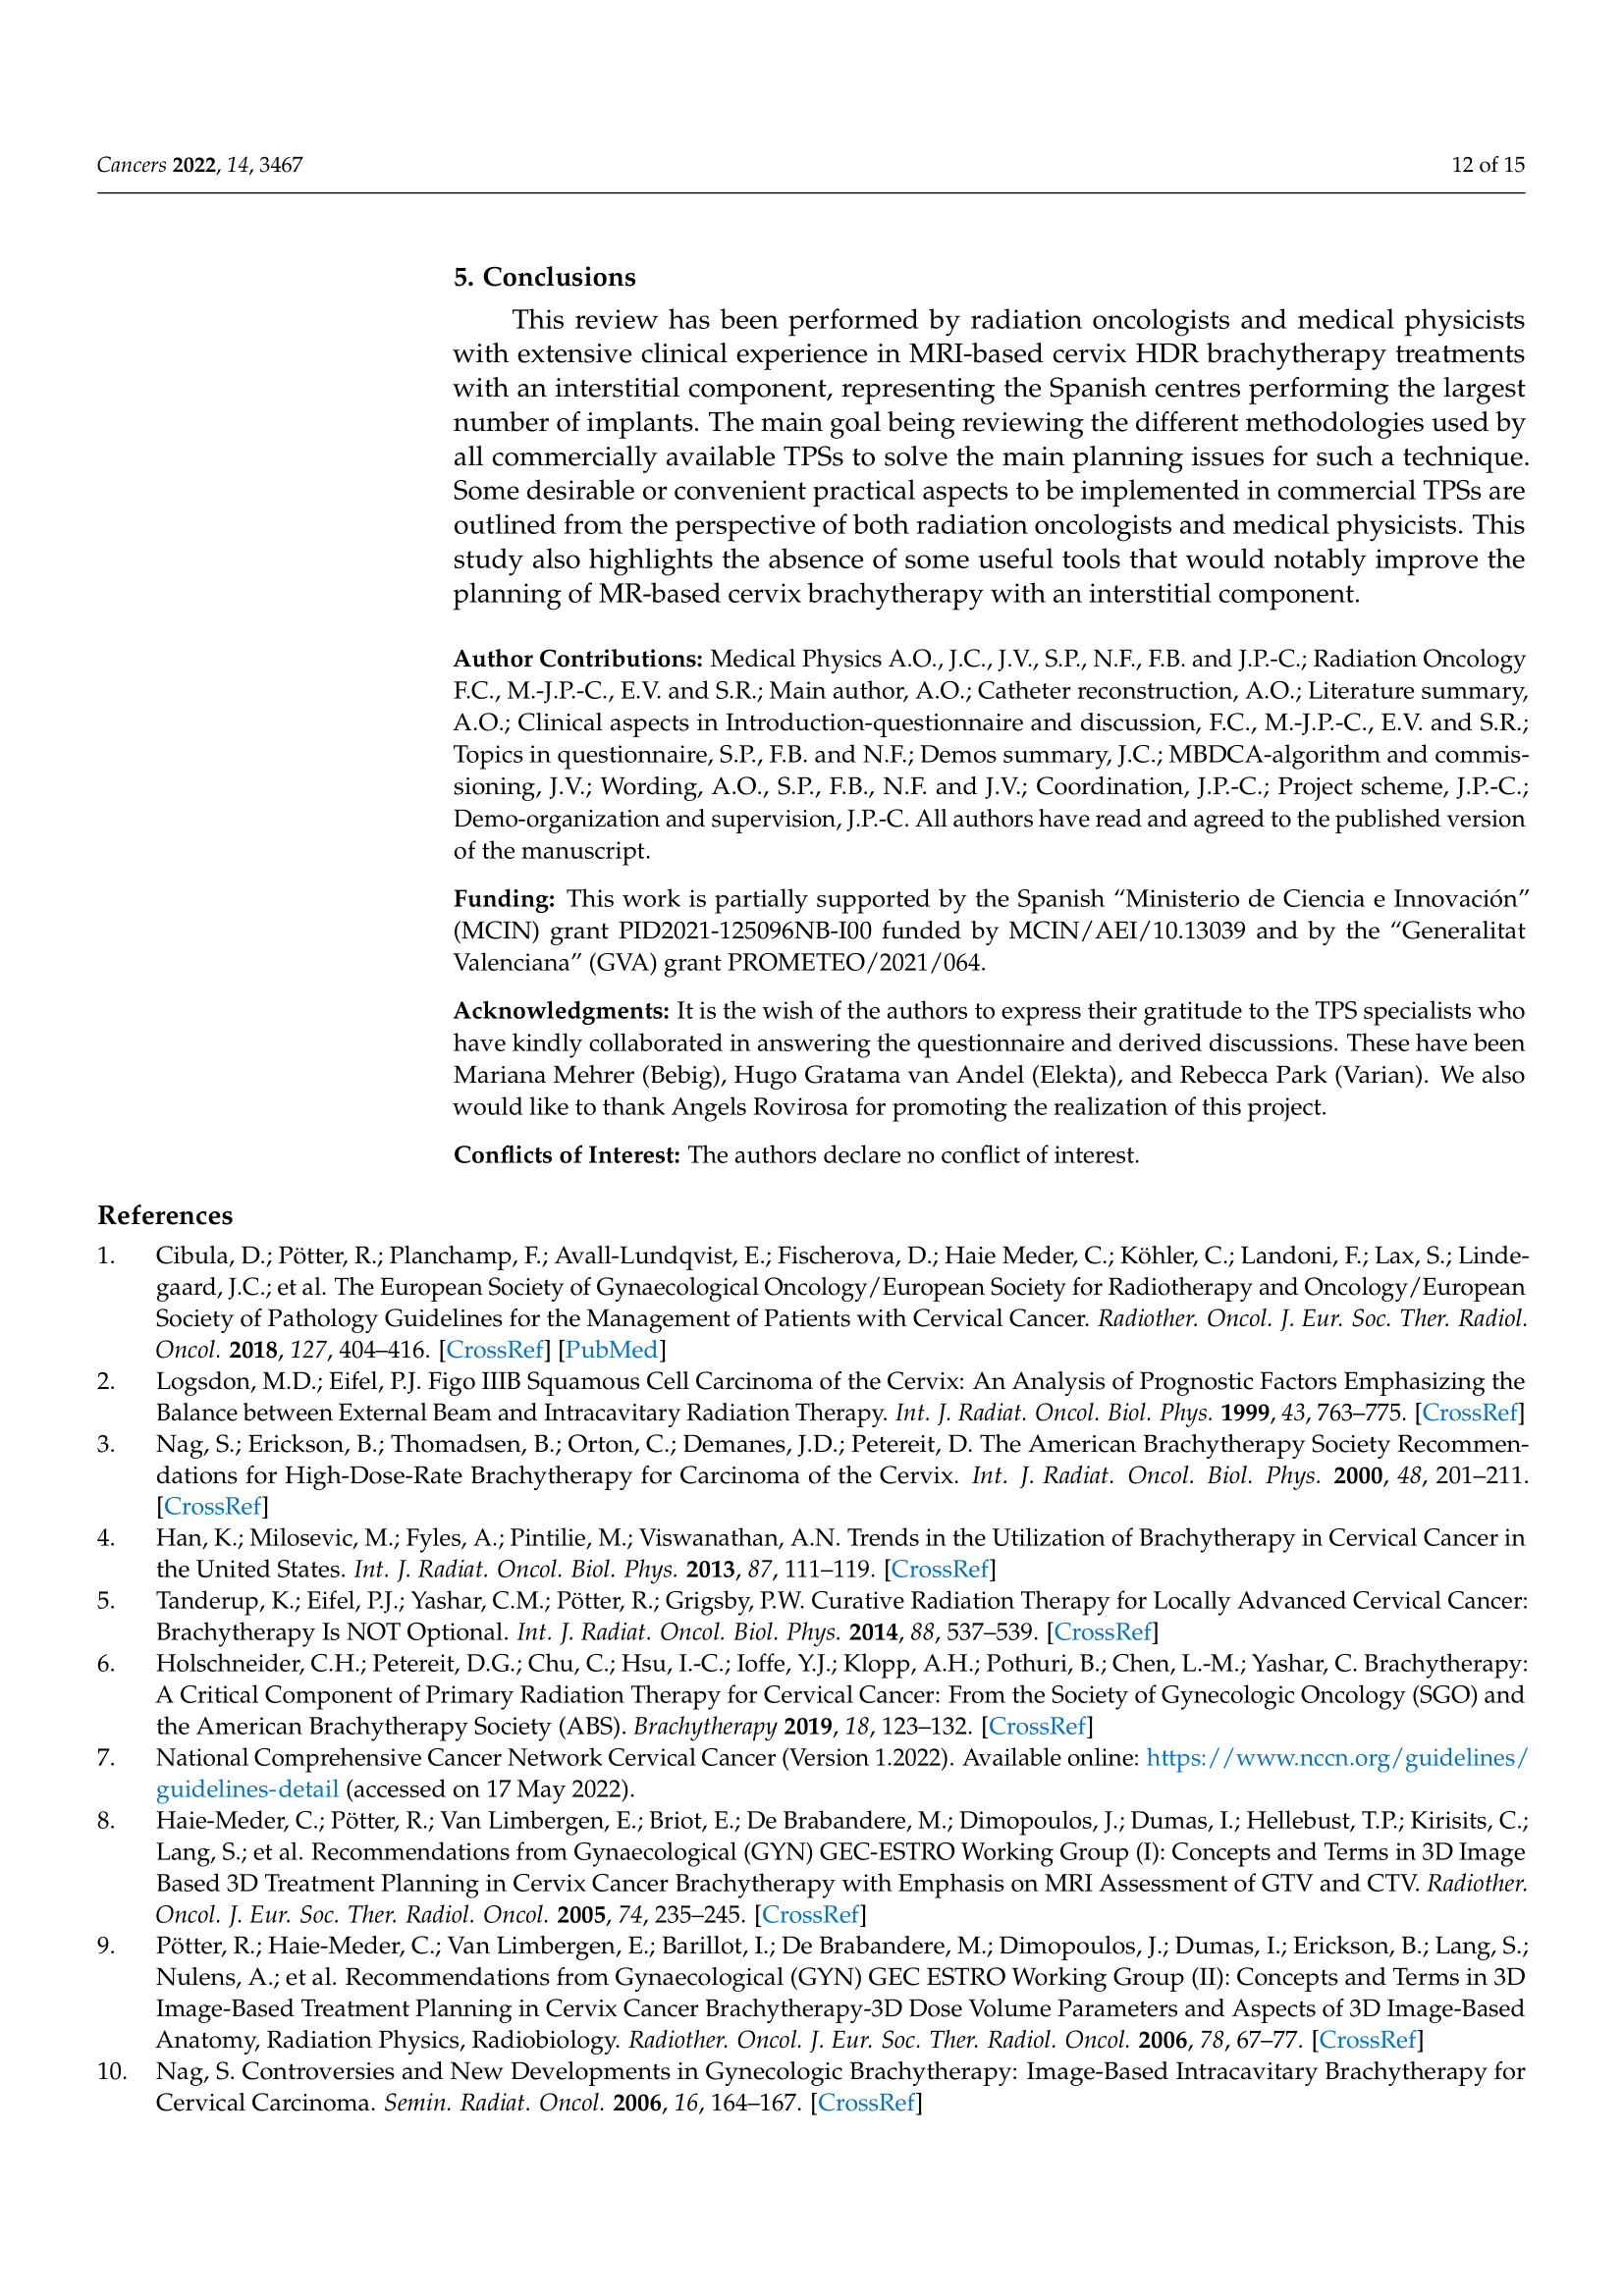
\includegraphics{articulos/cancers/cancers-12.png}

\includegraphics{articulos/cancers/cancers-13.png}

\includegraphics{articulos/cancers/cancers-14.png}

\includegraphics{articulos/cancers/cancers-15.png}

\bookmarksetup{startatroot}

\hypertarget{discusiuxf3n}{%
\chapter{Discusión}\label{discusiuxf3n}}

\hypertarget{sec-discusionotal2017}{%
\section{A method to incorporate interstitial components into the TPS
gynecologic rigid applicator library (Otal2017 publicado en febrero de
2017)}\label{sec-discusionotal2017}}

Como se vio en la sección~\ref{sec-bibapp}, la reconstrucción basada en
bibliotecas de aplicadores no es posible en el caso de la componente
intersticial, ya que el aplicador completo puede no considerarse
rígido\textsuperscript{\protect\hyperlink{ref-hellebust2010}{61}}. Sin
embargo, mediante la aplicación del método expuesto en la
sección~\ref{sec-MM-reconstruction} es factible el uso de las
bibliotecas de aplicadores en la reconstrucción de agujas. Por lo tanto,
en este trabajo presentamos un método para incluir aplicadores
intersticiales en la biblioteca Oncentra TPS para reconstruir dichos
aplicadores como un todo con la parte de las agujas incluídas.

En el caso del aplicador Utrecht, la falta de \emph{dummies} dificulta
la reconstrucción de la parte intersticial. Como vimos en la
sección~\ref{sec-tiposreconstruccion}, la localización de la \emph{tip
position} de las agujas es esencial para una correcta reconstrucción,
pero el surco negro dejado por la aguja en la imagen en T2 no es
suficiente para la determinación de la punta de la aguja. Previamente al
desarrollo de la biblioteca presentada en este trabajo, se utilizaba el
siguiente procedimiento en la reconstrucción del aplicador de Utrecht:
Los canales de los catéteres de la sonda intrauterina y de los ovoides
se determinan con la ayuda de la \emph{dummy} descrita por
Pérez-Calatayud et
al\textsuperscript{\protect\hyperlink{ref-puxe9rez-calatayud2011}{113}}.Las
agujas se reconstruyeron utilizando la metodología descrita en
Pérez-Calatayud et
al\textsuperscript{\protect\hyperlink{ref-perez-calatayud2011}{114}}. El
procedimiento consiste en utilizar la información de profundidad de
inserción, es decir, la profundidad desde la superficie del ovoide hasta
la punta de la aguja, dato proporcionado por el oncólogo radioterapeuta.
A continuación, se coloca en el plano reconstruido una regla de software
ajustada a la profundidad de inserción y se utiliza para definir los
diferentes puntos del catéter, incluidas las puntas de las agujas. Como
se ha indicado anteriormente, la profundidad de inserción reproducida
mediante la regla del programa informático corresponde a la distancia
desde la superficie del ovoide, pero con un desplazamiento de -0,7 cm,
para tener en cuenta la distancia máxima entre la fuente y el indexador
de 129 cm en el cargador posterior (microSelectron, versión 2 o 3 de
Elekta). Este procedimiento es laborioso e implica cierta incertidumbre
en el ajuste del punto de salida de la aguja del ovoide, unido a la
suposición de que la aguja es perfectamente recta.

En opinion de nuestro grupo, el uso de la biblioteca desarrollada mejora
significativamente la eficacia en la reconstrucción. En primer lugar, se
selecciona un aplicador virtual configurado en función de las
profundidades de las agujas; la posición de la parte intracavitaria se
establece sin grandes dificulades con la ayuda de las \emph{dummies} de
la parte intracavitaria y la superficie visible del modelo virtual del
aplicador. Una vez establecidos los ovoides, los puntos de salida de las
agujas quedan determinados y sólo se necesitan ligeras correcciones de
las agujas virtuales para ajustar su posición en función de la señal de
vacío que se ve sobre la MRI.

Para la evaluación del incremento en la precisión , se utilizaron ambos
métodos de reconstrucción en tres planos diferentes. Uno de los
beneficios del nuevo método propuesto se evidencia en la determinación
más precisa de la punta para la parte intracavitaria, reduciendo la
incertidumbre de 2 mm debida al efecto de volumen parcial por el grosor
del corte de la MRI. En el caso de las agujas, la reducción de las
incertidumbres debidas al límite del espesor de corte vienen de la más
precisa determinación del punto de salida de los ovoides. Las mayores
desviaciones en la determinación de la punta de la aguja se deben a la
suposición de agujas perfectamente rectas. Utilizando la biblioteca
desarrollada, también es posible modificar la curvatura de la aguja
virtual para que se ajuste mejor a las trayectorias reales sobre la
imagen.

En el caso del TB, que utiliza agujas de titanio, la reconstrucción se
basaba normalmente en los artefactos creados por la aguja en las
imágenes de las secuencias T1, utilizando el vacío creado como posición
de la punta de la aguja. Sin embargo, los tejidos que rodean las agujas
pueden presentar heterogeneidades que complican la identificación
precisa de estos patrones de artefactos, aumentando dicha dificultad en
las secuencias T2, que es la secuencia utilizada para la delimitación
del tumor\textsuperscript{\protect\hyperlink{ref-dimopoulos2012}{35}}.

Con el nuevo método presentado aquí, el tiempo necesario para
identificar las posiciones de las agujas se reduce considerablemente,
por debajo de un 50\%. El aplicador virtual con la profundidad de aguja
requerida se selecciona en Oncentra y, utilizando las tres bolas de
vitamina A como guías, se fija en el estudio de imagen T2 de RMN. A
continuación, cada orientación de la aguja se establece utilizando sólo
una imagen de plano axial, en la que el vacío en la punta de la aguja de
titanio es claramente visible con un buen contraste. Típicamente, sólo
dos planos axiales son suficientes para fijar todas las agujas. Las
ventajas de este enfoque para la TB son el ahorro de tiempo (como se ha
dicho anteriormente por debajo del 50\%, promediando el tiempo medido
para diferentes casos y diferentes físicos) y la reducción de la
probabilidad de identificación errónea del catéter, que puede ser un
problema debido al gran número de agujas que se suelen utilizar en la
práctica clínica (mínimo 14 agujas).

El método aquí propuesto es específico para el TPS Oncentra y para los
aplicadores Elekta Utrecht y TB. No obstante, el método es extensible a
otros planificadores que posean librerías de aplicadores y otros
aplicadores intersticiales distintos de los utilizados.

\hypertarget{pre-plan-technique-feasibility-in-multi-interstitialendocavitary-perineal-gynecological-brachytherapy-rodriguez2017-publicado-en-octubre-2017-2}{%
\section{Pre-plan technique feasibility in
multi-interstitial/endocavitary perineal gynecological brachytherapy
(Rodriguez2017 publicado en octubre
2017)}\label{pre-plan-technique-feasibility-in-multi-interstitialendocavitary-perineal-gynecological-brachytherapy-rodriguez2017-publicado-en-octubre-2017-2}}

El procedimiento de preplanificación virtual presenta ventajas
significativas: estimación de la profundidad de las agujas, posición y
número de las mismas, optimización de la cobertura del CTV y
minimización de las dosis en los órganos de riesgo. ``Un implante
subóptimo nunca puede transformarse en una aplicación satisfactoria
mediante ninguna forma de optimización de la planificación del
tratamiento''\textsuperscript{\protect\hyperlink{ref-gecestrohandbook2002}{115}}.
Las correcciones son limitadas en los casos de una dosimetría subóptima
debida a un volumen de tratamiento no cubierto. La planificación del
tratamiento basada exclusivamente en MR es preferible a otras
modalidades de imagen empleadas tradicionalmente, como el CT o los
métodos que utilizan registro de imágenes. Las incertidumbres se reducen
con la MR exclusiva ya que evitan imprecisiones derivadas de los
procedimientos de registro
TC-RM\textsuperscript{\protect\hyperlink{ref-hellebust2010}{61}}. En
consecuencia, ha crecido el interés por desarrollar dispositivos
totalmente compatibles con la MR que permitan la inserción y el guiado
en tiempo real de los aplicadores de
BT\textsuperscript{\protect\hyperlink{ref-viswanathan2006}{116}} . Una
alternativa es un plan virtual, o pre-plan, previo al tratamiento que
simule la configuración óptima del aplicador. La principal limitación
del pre-plan es la ausencia de la parte intracavitaria durante la
adquisición de las imágenes anteriores al tratamiento. También la
previsión de la divergencia que tomarán las agujas, sobre todo en el
caso de agujas no rígidas. La posición del útero varía en la mayoría de
las pacientes, siendo recto tras la inserción de la sonda intrauterina.
El pre-plan puede realizarse con componente intracavitaria bajo
anestesia
general\textsuperscript{\protect\hyperlink{ref-fokdal2013}{117}} o
paravaginal\textsuperscript{\protect\hyperlink{ref-petric2014c}{118}}. A
pesar de un pre-plan virtual, estos autores describen como un sexto de
todas las agujas planificadas e implantadas fueron agujas libres, es
decir, que no pertenecían a la plantilla debido a la limitación
geométrica del
anillo\textsuperscript{\protect\hyperlink{ref-fokdal2013}{117}}. Las
plantillas perineales como la TB evitan las limitaciones anteriores
debidas al uso de agujas rígidas, pudiendo añadir un componente
intrauterino y cubrir todas las direcciones de extensión del tumor.

Este procedimiento de planificación previa se ha aplicado con éxito en
10 pacientes consecutivas. Se ha logrado una excelente reproducción de
la planificación previa virtual. Cuando se trata a pacientes
histerectomizadas, sólo hay un pequeño cambio del pre-plan al post-plan.
Según nuestra experiencia, en pacientes sin cirugía, los cambios de
agujas también son pequeños, tanto en número como en posición tras la
inserción (dentro de 5 mm en la punta para una profundidad típica de 160
mm). El mismo oncólogo radioterapeuta experimentado ha realizado la
segmentación de los volúmenes tanto en la MR previa a la BT como en la
MR posterior al implante. En nuestra opinión, esta técnica de
pre-planificación virtual puede extenderse fácilmente a otros
aplicadores multi-intersticiales como MUPIT o Syed, con un número
optimizado de agujas y una profundidad adecuada. La planificación previa
y la biblioteca permiten un implante fácil y una reconstrucción rápida y
eficiente.

\hypertarget{review-on-treatment-planning-systems-for-cervix-brachytherapy-interventional-radiotherapy-some-desirable-and-convenient-practical-aspects-to-be-implemented-from-radiation-oncologist-and-medical-physics-perspectives-otal2022-publicado-en-julio-2022-2}{%
\section{Review on Treatment Planning Systems for Cervix Brachytherapy
(Interventional Radiotherapy): Some Desirable and Convenient Practical
Aspects to Be Implemented from Radiation Oncologist and Medical Physics
Perspectives (Otal2022 publicado en julio
2022)}\label{review-on-treatment-planning-systems-for-cervix-brachytherapy-interventional-radiotherapy-some-desirable-and-convenient-practical-aspects-to-be-implemented-from-radiation-oncologist-and-medical-physics-perspectives-otal2022-publicado-en-julio-2022-2}}

El principal objetivo de este estudio es proponer mejoras y señalar las
lagunas de los TPSs existentes, pero no cuantificar sus consecuencias.
Se excluyeron del estudio los paquetes de software externos compatibles
con los TPS que podrían ayudar a mejorar los problemas aquí señalados,
incluidos los entornos de scripting dentro de los TPS que pueden
permitir al usuario programar herramientas personalizadas. Como se ha
comentado anteriormente, esta revisión se basa en la experiencia clínica
de un grupo de oncólogos radioterápicos y físicos médicos. También se
utilizaron demostraciones interactivas proporcionadas por los
fabricantes de software e impartidas por especialistas de las empresas
proveedoras. Se pidió a estos especialistas que propusieran soluciones a
algunos de los retos mediante un cuestionario. Las posibles limitaciones
de esta metodología son las siguientes. Se basa en la opinión de
expertos y especialistas, por lo que los sesgos personales pueden estar
presentes. No obstante, teniendo en cuenta que se trata de un grupo
relativamente grande de profesionales que trabajan en diferentes
instituciones (diferentes protocolos, instalaciones, formación, etc.),
se minimiza el citado sesgo. Otra posible limitación es el hecho de que
no todos los expertos hayan utilizado todos los TPS en su práctica
clínica, algo inevitable teniendo en cuenta las realidades de la
práctica clínica. El uso de cuestionarios también podría limitar el
estudio, ya que intrínsecamente tienen sesgos de selección y muestreo
que podrían impedir el descubrimiento de situaciones imprevistas.

El paquete de software Velocity (Varian Medical Systems, Palo Alto, CA,
USA) incorpora herramientas más avanzadas para el registro de imágenes
que incluyen utilidades para la suma de dosis entre diferentes
fracciones. Sería deseable que estas herramientas, o similares, acabaran
llegando a los TPS de BT.

Otras herramientas, esta vez relacionadas con la segmentación de
volúmenes clínicos y órganos en riesgo, que sería interesante incorporar
a los TPS específicos de BT automatizarían dicha segmentación mediante
redes neuronales convolucionales. Éstas ya se están incorporando al
flujo de trabajo clínico en radioterapia, y existen trabajos recientes
en la literatura orientados explícitamente al caso del
cérvix\textsuperscript{\protect\hyperlink{ref-ma2021}{119}--\protect\hyperlink{ref-wang2020}{121}},
aunque el CT es la modalidad de imagen utilizada en estos trabajos.

Un tema apasionante en radioterapia externa es la generación de CT
sintéticos a partir de MRI. El objetivo principal de la generación de
estos CT es segmentar los tumores y órganos de riesgo en la RM y obtener
las densidades electrónicas necesarias para el cálculo de la
dosis\textsuperscript{\protect\hyperlink{ref-boulanger2021}{122}}. Estos
CT sintéticos podrían ser útiles en el caso de la BT cervical y
constituyen hoy en día una línea de investigación todavía por explorar.

La comunidad de usuarios ha desarrollado históricamente herramientas
``caseras'' que intentan compensar las deficiencias de los TPS y que
normalmente no pueden incorporarse al flujo de trabajo del planificador.
Un ejemplo comúnmente conocido son las hojas de cálculo. Un entorno de
scripting robusto en un lenguaje de alto nivel ayudaría a los usuarios a
optimizar sus rutinas de trabajo y también sería una fuente de
inspiración para los desarrolladores de nuevos productos para la
práctica clínica.

En los últimos años, varios grupos de investigación han estado
trabajando en sistemas de seguimiento
electromagnético\textsuperscript{\protect\hyperlink{ref-beld2018}{123}--\protect\hyperlink{ref-vanheerden2021}{125}}
para comprobar la trayectoria de la fuente de BT antes de la
administración del tratamiento. Uno de los especialistas entrevistado en
miembro de un grupo que está desarrollando dicha tecnología. Aunque su
finalidad principal es verificar la trayectoria seguida, en el futuro
podría utilizarse como herramienta de autorreconstrucción. En la
actualidad, no está a disposición de los usuarios.

Por último, recientemente se han publicado algunos estudios que
investigan la viabilidad de algoritmos basados en aprendizaje profundo
para la reconstrucción semiautomatizada de catéteres intersticiales
durante la HDR ginecológica basada en
MR\textsuperscript{\protect\hyperlink{ref-shaaer2021}{105}}.

\hypertarget{discusiuxf3n-general}{%
\section{Discusión general}\label{discusiuxf3n-general}}

El orden cronológico de la discusión de cada una de las publicaciones
incluídas en este texto obedece, además de a la lógica , a la intención
de justificar el por qué de la aparición de cada una de ellas.

La participación en dos publicaciones previas,por un lado la de
Rodriguez et
al\textsuperscript{\protect\hyperlink{ref-villalba2015}{79}} y por otra
la de Richart et
al\textsuperscript{\protect\hyperlink{ref-richart2015}{83}} son el punto
de partida del primero de los artículos publicados. En el primero de
ellos, se presenta el aplicador Benidorm
(sección~\ref{sec-templatebenidorm}). Va a ser diseñado para tumores
ginecológicos, con un enfoque especial en el carcinoma de cérvix
localmente avanzado. Este dispositivo permite la combinación de
radioterapia intracavitaria y agujas intersticiales compatibles con MRI.
El diseño del aplicador aborda las limitaciones de los aplicadores
comerciales existentes, como la incapacidad del componente
intracavitario para llegar profundamente al cuello uterino y la
incompatibilidad con MRI. Su diseño se orienta al tratamiento de
carcinomas cervicales avanzados con invasión parametrial voluminosa,
enfermedad primaria extensa que responde mal a la radioterapia externa,
y para casos con invasión paravaginal extensa. Es precisamente su diseño
orientado a su uso exclusivo con MRI lo que originó la segunda de las
publicaciones. En la publicación de Richart et al, se abordan los
problemas de reconstrucción de agujas de titanio en el contexto del uso
del aplicador Benidorm para implantes intersticiales en radioterapia.

Los implantes intersticiales a menudo utilizan agujas de titanio que son
difíciles de reconstruir con precisión en MRI. Para resolver este
problema, se propone un método que utiliza pequeños marcadores vitamina
A fácilmente visibles en imágenes de MRI para ayudar en la
reconstrucción de las agujas. Este método se aplica tanto en secuencias
T1 como T2 y se evaluó su consistencia mediante la reconstrucción de
varios implantes por dos físicos médicos con experiencia. Los resultados
mostraron diferencias de posicionamiento menores a 1 mm en todos los
casos. Además, este método permite usar solo la secuencia T2 para
contorneo o reconstrucción. A raiz del atículo de Richart et al y
uniendo las soluciones expuestas en él con la librería de aplicadores
del TPS Oncentra el resultado es la publicación
Otal2017\textsuperscript{\protect\hyperlink{ref-otal2017}{80}}. En él,
como hemos visto, además de modificar el modelo de aplicador Utrecht de
la biblioteca para añadir la parte instersticial, se introduce un
aplicador nuevo en la misma, el aplicador Benidorm.

La inclusión del aplicador Benidorm en la biblioteca de Oncentra sugiere
la posibilidad de utilizar el modelo virtual de dicho aplicador como una
manera de diseñar la carga de agujas y la profundidad de inserción
aprovechando la MR previa al tratamiento que ya se hacía con el mismo
propósito pero confiando en la experiencia del oncólogo que, después del
visionado de la MRI, determinaba la configuración del template el día
del implante. La utilización de el modelo virtual dota al equipo formado
por el físico médico y el oncólogo de una herramienta más sofisticada
para la realización de un implante adecuado.

Por otro lado, la idea de las bolas de vitamina A como marcadores
expuesta en la publicación de Richart et
al.\textsuperscript{\protect\hyperlink{ref-richart2015}{83}} va a ser
explorada en trabajos posteriores. En la publicación de Otal et
al.\textsuperscript{\protect\hyperlink{ref-otal2017}{80}} se describe la
inclusión en el modelo de la biblioteca de aplicadores del TPS Sagiplan
(Eckert \& Ziegler BEBIG, Berlin, Alemania) de tres marcadores esféricos
de vitamina A. La posición precisa de las esferas con respecto a la
geometría del aplicador es conocida ya que se diseñaron unos soportes
para dichas esferas que se añadieron al modelo
(figura~\ref{fig-viena1}). Dichos soportes se fabricaron con el uso de
una impresora 3D hechas de ácido poliláctido (PLA). La colocación de los
accesorios en el aplicador es sencilla y no afecta la integridad ni
otras características del producto. Las esferas son visibles en la MRI y
permiten el posicionamiento del aplicador sobre la imagen
(figura~\ref{fig-viena2}).

\begin{figure}

\begin{minipage}[t]{\linewidth}

{\centering 

\raisebox{-\height}{

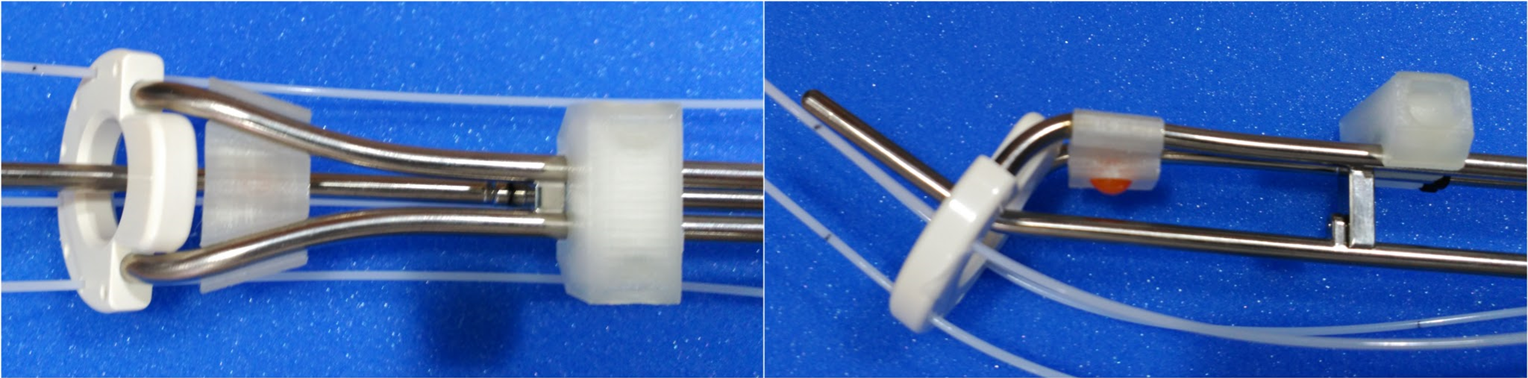
\includegraphics{img/viena1.png}

}

}

\subcaption{\label{fig-viena1}Soportes para las bolas de vitamina A
montados sobre el aplicador}
\end{minipage}%
\newline
\begin{minipage}[t]{\linewidth}

{\centering 

\raisebox{-\height}{

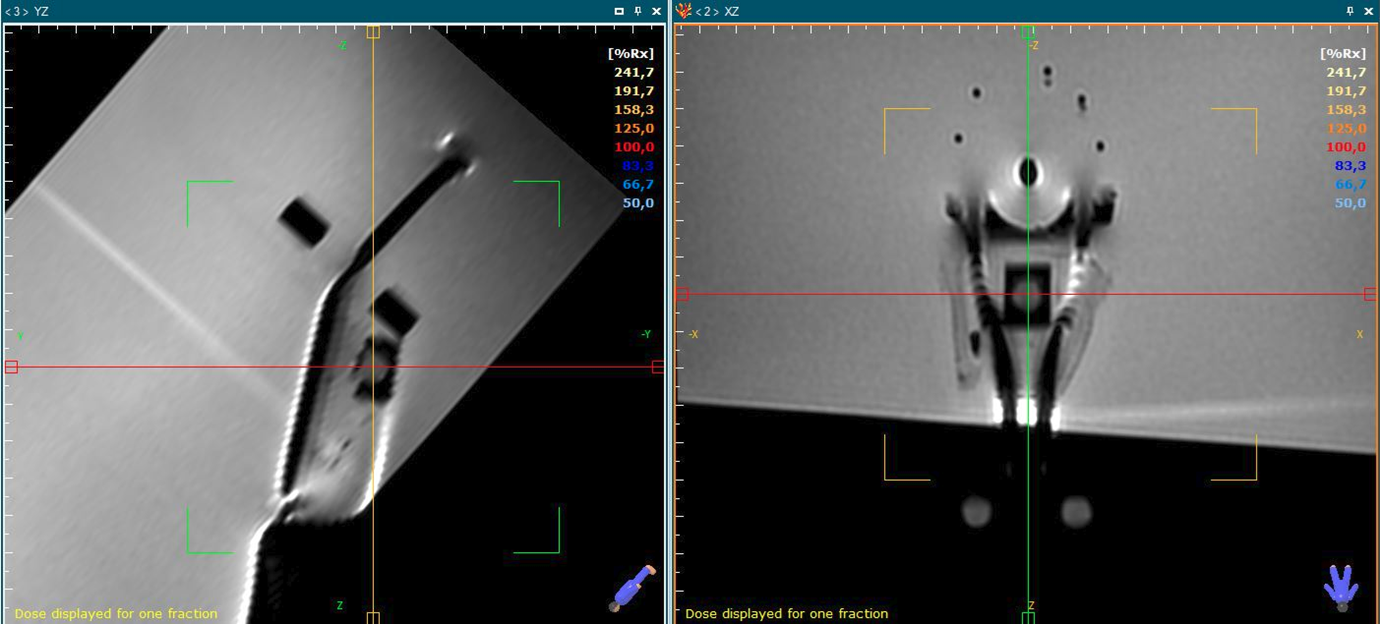
\includegraphics{img/viena2.png}

}

}

\subcaption{\label{fig-viena2}Detalle de las esferas sobre la imagen en
Sagiplan}
\end{minipage}%

\caption{\label{fig-viena}Aplicador Vienna en MRI}

\end{figure}

En 2018 Richart et
al.\textsuperscript{\protect\hyperlink{ref-richart2018}{34}} publicaron
un artículo de revisión en donde se intentó recopilar el estado del arte
de la reconstrucción de aplicadores en BT de cérvix. Entre otras muchas
fueron incluidas las descritas en lo párrafos anteriores de la sección.

En el trabajo de Otal et
al.\textsuperscript{\protect\hyperlink{ref-otal2019_plastic}{126}}, el
aplicador objetivo es el modelo Utrecht de la compañía Elekta
(Estocolmo, Suecia), un aplicador plástico. Utilizando las
\emph{dummies} del artículo de Pérez-Calatayud et
al.\textsuperscript{\protect\hyperlink{ref-perez-calatayud2009}{78}} se
obtienen las trayectorias de las fuentes en los tres canales
intracavitarios. Con esa información y por un método de mínimos
cuadrados se obtiene un modelo geométrico del aplicador adaptado al
implante, con lo que el aplicador podrá ser colocado sobre la MRI como
si fuese un aplicador de una sola pieza.

Se aplicó el método expuesto a 14 pacientes con caracter retrospectivo.
Las distancias entre los puntos en la imagen y los calculados se muestra
en el histograma de la figura~\ref{fig-utrecht1}. En el caso de los
ovoides, las diferencias están por debajo del milímetro, no así en el
caso de la sonda intrauterina, en el que no se aprecian tan buenos
resultados. El peor resultado para la sonda intrauterina es debido a la
menor curvatura de la misma lo que hace que en el ajuste exista una
indeterminación mayor que en el caso de los ovoides los cuales forman un
ángulo que minimiza la incertidumbre en la dirección cráneo-caudal.

\begin{figure}

{\centering 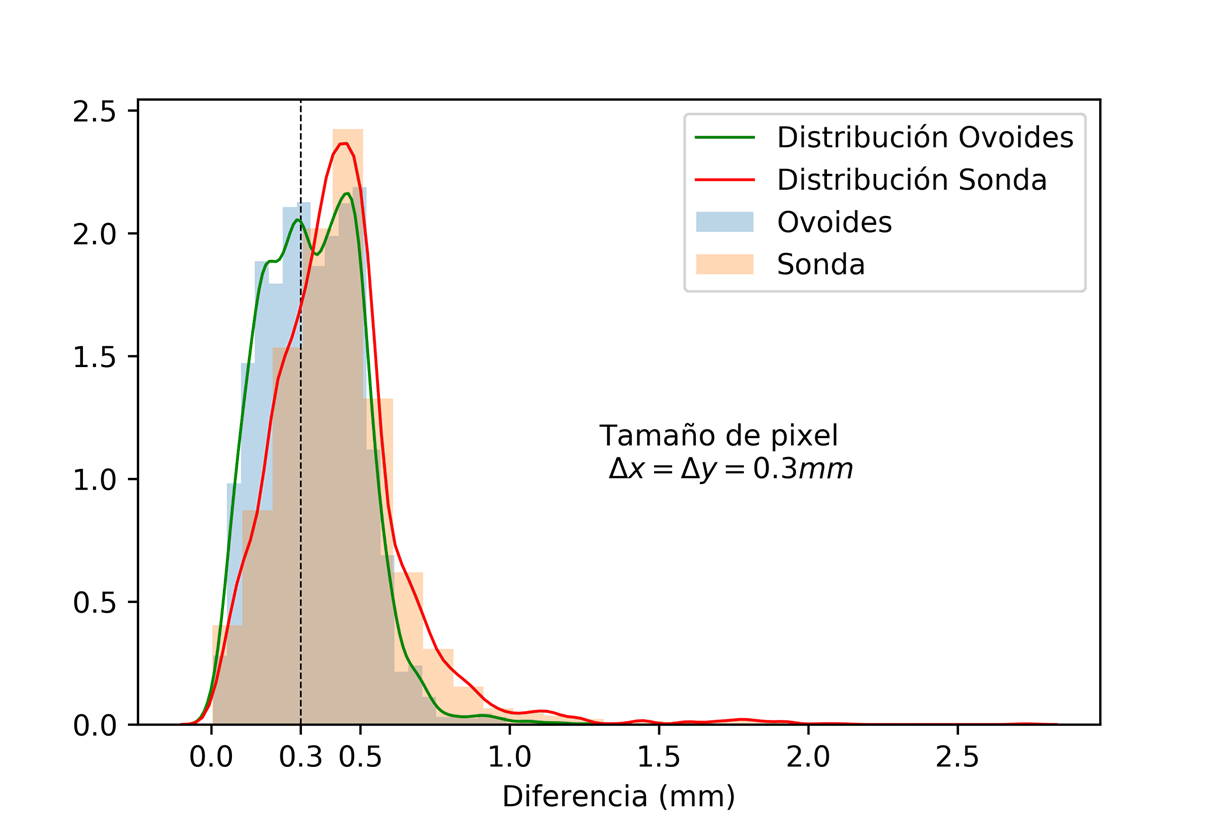
\includegraphics{img/utrecht1.png}

}

\caption{\label{fig-utrecht1}Histograma de distancias entre los canales
en la MRI y las obtenidas mediante la transformación del modelo de la
biblioteca}

\end{figure}

El método descrito en Otal et
al.\textsuperscript{\protect\hyperlink{ref-otal2019_plastic}{126}} es de
uso exclusivo para aplicadores plásticos, ya que las \emph{dummies} del
canal son visibles en la MRI. No así para aplicadores metálicos en donde
una \emph{dummy} de ese tipo no es viable. En el trabajo de Otal et
al.\textsuperscript{\protect\hyperlink{ref-otal2019_metal}{127}}, se
propone un método diferente adaptado a los aplicadores metálicos,
concretamente en el aplicador Fletcher (Mick, Eckert\&Ziegler, Germany).
Dicho método se basa en obtener medidas de distancias en el aplicador ya
implantado y mediante esta parametrización obtener un modelo virtual
para la biblioteca del aplicador completo y tratarlo como si fuese
rígido, al igual que se hizo para el aplicador Utrecht
(figura~\ref{fig-fletcher}).

\begin{figure}

\begin{minipage}[t]{\linewidth}

{\centering 

\raisebox{-\height}{

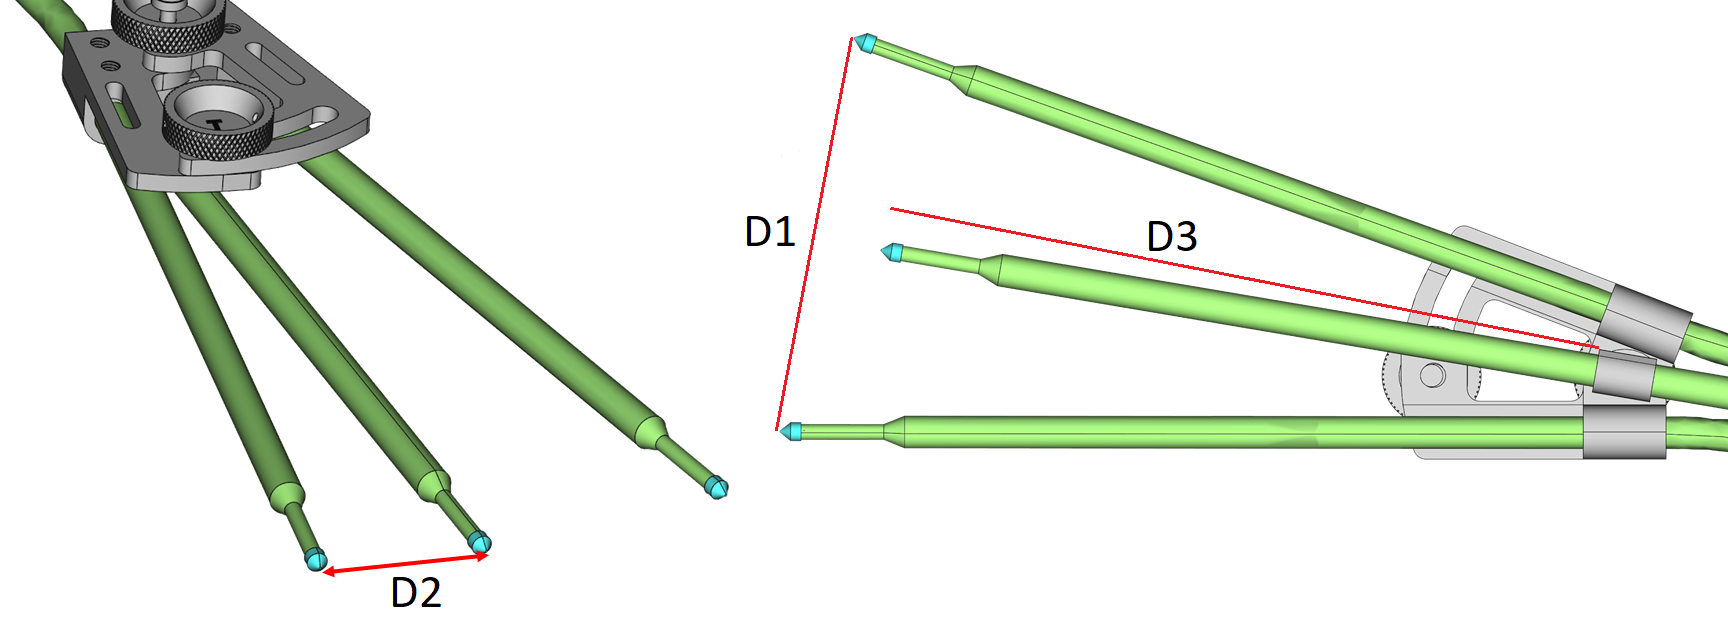
\includegraphics{img/fletcher2.png}

}

}

\subcaption{\label{fig-fletcher1}Detalle de los parámetros de distancia
sobre un modelo de CAD}
\end{minipage}%
\newline
\begin{minipage}[t]{\linewidth}

{\centering 

\raisebox{-\height}{

\includegraphics{img/fletcher1.png}

}

}

\subcaption{\label{fig-fletcher2}Aplicador sobre la imagen desde la
biblioteca de aplicadores de Sagiplan}
\end{minipage}%

\caption{\label{fig-fletcher}Aplicador Fletcher de Mick}

\end{figure}

Posteriormente, en el año 2021 Otal et
al.\textsuperscript{\protect\hyperlink{ref-otal2021}{128}} presentaron
una herramienta para facilitar y ampliar la reconstrucción de apicadores
plásticos sobre MRI, nuevamente sobre el aplicador Utrecht. Dicha
herramienta está desarrollada sobre la plataforma
3DSlicer\textsuperscript{\protect\hyperlink{ref-fedorov2012}{129}} y
además de las soluciones aportadas en Otal et
al.\textsuperscript{\protect\hyperlink{ref-otal2019_plastic}{126}}, ha
sido añadida una herramienta que permite la reconstrucción de la parte
intersticial a partir de la parte intracavitaria. Las ideas principales
para la construcción de la herramienta son las aportadas en el artículo
de Otal et al.\textsuperscript{\protect\hyperlink{ref-otal2017}{80}}

Una vez posicionada la parte intracavitaria se seleccionan en un
desplegable las agujas colocadas en el implante y se introduce el valor
de la profundidad de cada una de ellas, valor registrado por el
responsable del implante (figura~\ref{fig-utrecht2}). El punto de salida
de cada una de las agujas es conocido de la parte intracavitaria, esto
unido a los puntos registrados sobre la imagen de cada una de las agujas
es ajustado a un spline polinómico que tiene la longitud aportada
anteriormente (figura~\ref{fig-utrecht3}).

\begin{figure}

\begin{minipage}[t]{\linewidth}

{\centering 

\raisebox{-\height}{

\includegraphics{img/utrecht2.png}

}

}

\subcaption{\label{fig-utrecht2}Formulario con la información del
implante}
\end{minipage}%
\newline
\begin{minipage}[t]{\linewidth}

{\centering 

\raisebox{-\height}{

\includegraphics{img/utrecht3.png}

}

}

\subcaption{\label{fig-utrecht3}Vista en 3DSlicer del implante completo}
\end{minipage}%

\caption{\label{fig-utrecht}Herramienta en 3DSlicer para la
reconstrucción del aplicador Utrecht}

\end{figure}

La herramienta desarrollada es ajena a la biblioteca de aplicadores de
Oncentra, ya que contiene los modelos tridimensionales del aplicador en
ella y por tanto es posible introducirlo en una versión de Oncentra sin
la licencia de la biblioteca, la cual no viene incluída con el paquete
básico. La salida que aporta son las coordenadas de cada punto de parada
de la fuente para todos los canales del aplicador, tanto los
intracavitarios como los intersticiales. Dichos valores se pueden
introducir en el planificador a mano, lo cual es bastante tedioso y con
peligro de cometer errores de transcripción o diseñar algún
procedimiento de exportación de ficheros que permita al planificador
importarlo de manera automática. El procedimiento completo de
reconstrucción se puede visionar en la plataforma de vídeos
\href{https://youtu.be/kv827vIsAZM}{Youtube}. Además de como herramienta
de reconstrucción, también puede ser utilizada como herramienta de
anotación para que los ficheros resultantes puedan ser útiles como datos
para el entrenamiento de algoritmos de inteligencia artificial que
posibiliten el desarrollo de soluciones de autoreconstrucción.

El desarrollo de todas las innovaciones expuestas previamente unidas a
la inquietud sobre las carencias de los TPSs actuales de un grupo de
profesionales, físicos médicos y oncólogos radioterápicos, con sólida
experiencia en el tratamiento de tumores de cérvix en BT intersticial
con MRI exclusiva, fueron el germen de la publicación Otal et
al.\textsuperscript{\protect\hyperlink{ref-otal2022}{82}}

\bookmarksetup{startatroot}

\hypertarget{conclusiones}{%
\chapter{Conclusiones}\label{conclusiones}}

Si partimos del hecho de que la MRI es la modalidad de imagen óptima
para el tratamiento mediante BT del carcinoma de cérvix avanzado, la
reconstrucción exclusiva sobre MRI de aplicadores ginecológicos es una
alternativa robusta a la basada en registro de imágenes con CT. Es
evidente la reducción de las incertidumbres asociadas a la
reconstrucción exclusiva al eliminar las introducidas por los
procedimientos de registro de CT-MRI. Por otro lado, es innegable que la
peor visibilidad de los aplicadores ginecológicos en MRI, especialmente
de la parte intersticial, hace que la reconstrucción sobre dicha
modalidad de imagen introduzca nuevos retos. Dichos retos pueden ser
superados utilizando técnicas basadas en bibliotecas de aplicadores.

La reconstrucción de aplicadores intra-cavitarios mediante el uso de
bibliotecas de aplicadores se revela como una herramienta versátil que
puede extenderse a aplicadores que, aunque no sean estrictamente
rígidos, pueden configurarse como tales, adaptándose a la disposición
específica de cada implante. De esta manera al obtener un modelo de
aplicador configurado para un implante específico, no es necesario ver
explícitamente sobre la MRI los canales por donde circula la fuente,
siempre que haya otras partes visibles del aplicador sobre la imagen,
aunque estas sean periféricas. Más importante todavía es que un punto
tan crítico como es la \emph{tip-position} de cada canal puede ser
determinado gracias a la configuración conocida del aplicador. En el
concepto de aplicadores que no sean estrictamente rígidos podemos
incluir la parte intersticial aprovechando los puntos comunes de dicha
parte con la compartida con la intra-cavitaria y la medida de la
profundidad de inserción.

Aprovechando las técnicas descritas en el párrafo anterior donde
definimos un modelo de aplicador completo para un implante determinado,
podemos utilizar un modelo de este tipo sobre una imagen pre-implante y
probar dosimetrías previas al implante real. Las bibliotecas de
aplicadores utilizando el concepto anterior permiten la creación de
planes virtuales basados en imágenes previas al procedimiento
intervencionista. Este enfoque permite probar diferentes configuraciones
de la parte intersticial del aplicador buscando la que en opinión del
médico intervencionista sea la que resulte en un mejor compromiso de
cobertura de los volúmenes blanco y de la protección de los OAR. Estos
planes virtuales serían análogos a los utilizados con el mismo fin en
braquiterapia de próstata.

Lo peculiar de la BT de cérvix basada exclusivamente en MRI exige dotar
de nuevas herramientas a los TPS que ayuden a los profesionales a crear
tratamientos cada vez mejores que redunden en la calidad de los
tratamientos. Es de vital importancia que las casas comerciales que
comercializan los TPS tomen en cuenta las sugerencias y las carencias
señaladas por los físicos médicos y los oncólogos radioterápicos que
realizan los implantes de braquiterapia, pudiendo ser las herramientas
\emph{caseras} desarrolladas por la comunidad de usuarios una fuente de
inspiración. Nuevos avances como el seguimiento electromagnético o la
explosión de herramientas basadas en inteligencia artificial cuyos
resultados van desde la generación de CT sintéticos a partir de una MRI
a la segmentación automática de volúmenes (o de aplicadores) pueden
hacer evolucionar los TPS de braquiterapia en general y para el
tratamiento exclusivo con MRI del cáncer de cérvix en particular.

\bookmarksetup{startatroot}

\hypertarget{bibliografuxeda}{%
\chapter*{Bibliografía}\label{bibliografuxeda}}
\addcontentsline{toc}{chapter}{Bibliografía}

\markboth{Bibliografía}{Bibliografía}

\hypertarget{refs}{}
\begin{CSLReferences}{0}{0}
\leavevmode\vadjust pre{\hypertarget{ref-goodwin1968}{}}%
\CSLLeftMargin{1. }%
\CSLRightInline{Goodwin PN. Radium Dosage: The Manchester SystemRadium
Dosage: The Manchester System. Edited byMeredithW. J., D. Sc., F. Inst.
P. Compiled from articles byPatersonRalston,SpiersF. W.,StephensonS.
K,ParkerH. M.,TodM. C., andMeredithW. J.. Cloth, {\$}8.75; 42s. Pp. 170,
with 66 figures. Edinburgh, E. \& S. Livingstone; Baltimore, Md.,
Williams \& Wilkins Co., 2d ed., 1967. \emph{Radiology}.
1968;91(1):175-175.
doi:\href{https://doi.org/10.1148/91.1.175a}{10.1148/91.1.175a}}

\leavevmode\vadjust pre{\hypertarget{ref-adosage1934}{}}%
\CSLLeftMargin{2. }%
\CSLRightInline{A Dosage System for Gamma Ray Therapy. \emph{The British
Journal of Radiology}. 1934;7(82):578-579.
doi:\href{https://doi.org/10.1259/0007-1285-7-82-578}{10.1259/0007-1285-7-82-578}}

\leavevmode\vadjust pre{\hypertarget{ref-parker1938}{}}%
\CSLLeftMargin{3. }%
\CSLRightInline{Parker HM. A Dosage System for Interstitial Radium
Therapy. Part II{\textemdash}Physical Aspects. \emph{The British Journal
of Radiology}. 1938;11(125):313-340.
doi:\href{https://doi.org/10.1259/0007-1285-11-125-313}{10.1259/0007-1285-11-125-313}}

\leavevmode\vadjust pre{\hypertarget{ref-thetrea1949b}{}}%
\CSLLeftMargin{4. }%
\CSLRightInline{The Treatment of Malignant Disease by Radium and X-Rays,
Being a Practice of RadiotherapyThe Treatment of Malignant Disease by
Radium and X-Rays, Being a Practice of Radiotherapy. By PatersonRalston,
M.C., M.D., F.R.C.S.E., D.M.R.E., F.F.R., Christie Hospital and Holt
Radium Institute, Manchester. A volume of 622 pages, with numerous
figures, tables, and charts. Published by Butler and Tanner, Ltd., Frome
and London The Williams \& Wilkins Co., Baltimore, 1948. Price
{\$}11.00. \emph{Radiology}. 1949;52(1):125-125.
doi:\href{https://doi.org/10.1148/52.1.125a}{10.1148/52.1.125a}}

\leavevmode\vadjust pre{\hypertarget{ref-viswanathan2012a}{}}%
\CSLLeftMargin{5. }%
\CSLRightInline{Viswanathan AN, Beriwal S, De Los Santos JF, et~al.
American Brachytherapy Society consensus guidelines for locally advanced
carcinoma of the cervix. Part II: High-dose-rate brachytherapy.
\emph{Brachytherapy}. 2012;11(1):47-52.
doi:\href{https://doi.org/10.1016/j.brachy.2011.07.002}{10.1016/j.brachy.2011.07.002}}

\leavevmode\vadjust pre{\hypertarget{ref-williamson2006}{}}%
\CSLLeftMargin{6. }%
\CSLRightInline{Williamson JF. Brachytherapy technology and physics
practice since 1950: a half-century of progress. \emph{Physics in
Medicine and Biology}. 2006;51(13):R303-R325.
doi:\href{https://doi.org/10.1088/0031-9155/51/13/r18}{10.1088/0031-9155/51/13/r18}}

\leavevmode\vadjust pre{\hypertarget{ref-clinic2012}{}}%
\CSLLeftMargin{7. }%
\CSLRightInline{Comprehensive Brachytherapy - Clinical Use of
Brachytherapy. En: CRC Press; 2012:276-281.
doi:\href{https://doi.org/10.1201/b13075-26}{10.1201/b13075-26}}

\leavevmode\vadjust pre{\hypertarget{ref-jemal2008}{}}%
\CSLLeftMargin{8. }%
\CSLRightInline{Jemal A, Siegel R, Ward E, et~al. Cancer Statistics,
2008. \emph{CA: A Cancer Journal for Clinicians}. 2008;58(2):71-96.
doi:\href{https://doi.org/10.3322/ca.2007.0010}{10.3322/ca.2007.0010}}

\leavevmode\vadjust pre{\hypertarget{ref-singh2023}{}}%
\CSLLeftMargin{9. }%
\CSLRightInline{Singh D, Vignat J, Lorenzoni V, et~al. Global estimates
of incidence and mortality of cervical cancer in 2020: a baseline
analysis of the WHO Global Cervical Cancer Elimination Initiative.
\emph{The Lancet Global Health}. 2023;11(2):e197-e206.
doi:\href{https://doi.org/10.1016/s2214-109x(22)00501-0}{10.1016/s2214-109x(22)00501-0}}

\leavevmode\vadjust pre{\hypertarget{ref-introd2012}{}}%
\CSLLeftMargin{10. }%
\CSLRightInline{- Introduction and Innovations in Brachytherapy. En: CRC
Press; 2012:32-37.
doi:\href{https://doi.org/10.1201/b13075-9}{10.1201/b13075-9}}

\leavevmode\vadjust pre{\hypertarget{ref-aronowitz2015}{}}%
\CSLLeftMargin{11. }%
\CSLRightInline{Aronowitz JN. Afterloading: The Technique That Rescued
Brachytherapy. \emph{International Journal of Radiation
Oncology*Biology*Physics}. 2015;92(3):479-487.
doi:\href{https://doi.org/10.1016/j.ijrobp.2015.02.014}{10.1016/j.ijrobp.2015.02.014}}

\leavevmode\vadjust pre{\hypertarget{ref-tod1938}{}}%
\CSLLeftMargin{12. }%
\CSLRightInline{Tod MC, Meredith WJ. A Dosage System for Use in the
Treatment of Cancer of the Uterine Cervix. \emph{The British Journal of
Radiology}. 1938;11(132):809-824.
doi:\href{https://doi.org/10.1259/0007-1285-11-132-809}{10.1259/0007-1285-11-132-809}}

\leavevmode\vadjust pre{\hypertarget{ref-tod1953}{}}%
\CSLLeftMargin{13. }%
\CSLRightInline{Tod M, Meredith WJ. Treatment of Cancer of the Cervix
Uteri{\textemdash}A Revised {``}Manchester Method{''}. \emph{The British
Journal of Radiology}. 1953;26(305):252-257.
doi:\href{https://doi.org/10.1259/0007-1285-26-305-252}{10.1259/0007-1285-26-305-252}}

\leavevmode\vadjust pre{\hypertarget{ref-yordy2012}{}}%
\CSLLeftMargin{14. }%
\CSLRightInline{Yordy JS, Almond PR, Delclos L. Development of the M. D.
Anderson Cancer Center Gynecologic Applicators for the Treatment of
Cervical Cancer: Historical Analysis. \emph{International Journal of
Radiation Oncology*Biology*Physics}. 2012;82(4):1445-1453.
doi:\href{https://doi.org/10.1016/j.ijrobp.2011.05.029}{10.1016/j.ijrobp.2011.05.029}}

\leavevmode\vadjust pre{\hypertarget{ref-ICRU38}{}}%
\CSLLeftMargin{15. }%
\CSLRightInline{ICRU. \emph{ICRU Report 38: Dose and Volume
Specification for Reporting Intracavitary Therapy in Gynecology}.
International Commission on Radiation Units; Measurements; 1985.}

\leavevmode\vadjust pre{\hypertarget{ref-puxf6tter2001}{}}%
\CSLLeftMargin{16. }%
\CSLRightInline{Pötter R, Van Limbergen E, Gerstner N, Wambersie A.
Survey of the use of the ICRU 38 in recording and reporting cervical
cancer brachytherapy. \emph{Radiotherapy and Oncology}.
2001;58(1):11-18.
doi:\href{https://doi.org/10.1016/s0167-8140(00)00266-8}{10.1016/s0167-8140(00)00266-8}}

\leavevmode\vadjust pre{\hypertarget{ref-miyata2023}{}}%
\CSLLeftMargin{17. }%
\CSLRightInline{Miyata Y, Murakami N, Okuma K, et~al. Technical Note:
High-Dose-Rate Interstitial Brachytherapy for Pelvic Sidewall Recurrence
Using Intraperitoneal Spacers. \emph{Advances in Radiation Oncology}.
2023;8(1):101118.
doi:\href{https://doi.org/10.1016/j.adro.2022.101118}{10.1016/j.adro.2022.101118}}

\leavevmode\vadjust pre{\hypertarget{ref-onal2009a}{}}%
\CSLLeftMargin{18. }%
\CSLRightInline{Onal C, Arslan G, Topkan E, et~al. Comparison of
conventional and CT-based planning for intracavitary brachytherapy for
cervical cancer: target volume coverage and organs at risk doses.
\emph{Journal of Experimental \& Clinical Cancer Research}. 2009;28(1).
doi:\href{https://doi.org/10.1186/1756-9966-28-95}{10.1186/1756-9966-28-95}}

\leavevmode\vadjust pre{\hypertarget{ref-sagae2023}{}}%
\CSLLeftMargin{19. }%
\CSLRightInline{Sagae S, Toita T, Matsuura M, et~al. Improvement in
radiation techniques for locally advanced cervical cancer during the
last two decades. \emph{International Journal of Gynecologic Cancer}.
2023;33(8):1295-1303.
doi:\href{https://doi.org/10.1136/ijgc-2022-004230}{10.1136/ijgc-2022-004230}}

\leavevmode\vadjust pre{\hypertarget{ref-haie-meder2005}{}}%
\CSLLeftMargin{20. }%
\CSLRightInline{Haie-Meder C, Pötter R, Van Limbergen E, et~al.
Recommendations from Gynaecological (GYN) GEC-ESTRO Working Group☆ (I):
concepts and terms in 3D image based 3D treatment planning in cervix
cancer brachytherapy with emphasis on MRI assessment of GTV and CTV.
\emph{Radiotherapy and Oncology}. 2005;74(3):235-245.
doi:\href{https://doi.org/10.1016/j.radonc.2004.12.015}{10.1016/j.radonc.2004.12.015}}

\leavevmode\vadjust pre{\hypertarget{ref-charra-brunaud2012}{}}%
\CSLLeftMargin{21. }%
\CSLRightInline{Charra-Brunaud C, Harter V, Delannes M, et~al. Impact of
3D image-based PDR brachytherapy on outcome of patients treated for
cervix carcinoma in France: Results of the French STIC prospective
study. \emph{Radiotherapy and Oncology}. 2012;103(3):305-313.
doi:\href{https://doi.org/10.1016/j.radonc.2012.04.007}{10.1016/j.radonc.2012.04.007}}

\leavevmode\vadjust pre{\hypertarget{ref-mayadev2017}{}}%
\CSLLeftMargin{22. }%
\CSLRightInline{Mayadev J, Viswanathan A, Liu Y, et~al. American
Brachytherapy Task Group Report: A pooled analysis of clinical outcomes
for high-dose-rate brachytherapy for cervical cancer.
\emph{Brachytherapy}. 2017;16(1):22-43.
doi:\href{https://doi.org/10.1016/j.brachy.2016.03.008}{10.1016/j.brachy.2016.03.008}}

\leavevmode\vadjust pre{\hypertarget{ref-viswanathan2010}{}}%
\CSLLeftMargin{23. }%
\CSLRightInline{Viswanathan AN, Erickson BA. Three-Dimensional Imaging
in Gynecologic Brachytherapy: A Survey of the American Brachytherapy
Society. \emph{International Journal of Radiation
Oncology*Biology*Physics}. 2010;76(1):104-109.
doi:\href{https://doi.org/10.1016/j.ijrobp.2009.01.043}{10.1016/j.ijrobp.2009.01.043}}

\leavevmode\vadjust pre{\hypertarget{ref-dimopoulos2006}{}}%
\CSLLeftMargin{24. }%
\CSLRightInline{Dimopoulos JCA, Kirisits C, Petric P, et~al. The Vienna
applicator for combined intracavitary and interstitial brachytherapy of
cervical cancer: Clinical feasibility and preliminary results.
\emph{International Journal of Radiation Oncology*Biology*Physics}.
2006;66(1):83-90.
doi:\href{https://doi.org/10.1016/j.ijrobp.2006.04.041}{10.1016/j.ijrobp.2006.04.041}}

\leavevmode\vadjust pre{\hypertarget{ref-vandyk2021}{}}%
\CSLLeftMargin{25. }%
\CSLRightInline{Dyk S van, Khaw P, Lin M-Y, Chang D, Bernshaw D.
Ultrasound-guided Brachytherapy for Cervix Cancer. \emph{Clinical
Oncology}. 2021;33(9):e403-e411.
doi:\href{https://doi.org/10.1016/j.clon.2021.02.011}{10.1016/j.clon.2021.02.011}}

\leavevmode\vadjust pre{\hypertarget{ref-van2015}{}}%
\CSLLeftMargin{26. }%
\CSLRightInline{Dyk S van, Schneider M, Kondalsamy-Chennakesavan S,
Bernshaw D, Narayan K. Ultrasound use in gynecologic brachytherapy: Time
to focus the beam. \emph{Brachytherapy}. 2015;14(3):390-400.
doi:\href{https://doi.org/10.1016/j.brachy.2014.12.001}{10.1016/j.brachy.2014.12.001}}

\leavevmode\vadjust pre{\hypertarget{ref-St-Amant2017}{}}%
\CSLLeftMargin{27. }%
\CSLRightInline{St-Amant P, Foster W, Froment MA, Aubin S, Lavallée MC,
Beaulieu L. Use of 3D transabdominal ultrasound imaging for treatment
planning in cervical cancer brachytherapy: Comparison to magnetic
resonance and computed tomography. \emph{Brachytherapy}.
2017;16(4):847-854.
doi:\href{https://doi.org/10.1016/j.brachy.2017.03.006}{10.1016/j.brachy.2017.03.006}}

\leavevmode\vadjust pre{\hypertarget{ref-ora2022}{}}%
\CSLLeftMargin{28. }%
\CSLRightInline{Ora M, Saini V, Markam K, Nazar A, Gambhir S. Relapsed
carcinoma cervix presented with multiple rare visceral metastases: Role
of 18f-fluorodeoxyglucose positron emission tomography/computed
tomography. \emph{Indian Journal of Nuclear Medicine}. 2022;37(4):373.
doi:\href{https://doi.org/10.4103/ijnm.ijnm_58_22}{10.4103/ijnm.ijnm\_58\_22}}

\leavevmode\vadjust pre{\hypertarget{ref-fracasso2022}{}}%
\CSLLeftMargin{29. }%
\CSLRightInline{Fracasso PM, Duska LR, Thaker PH, et~al. An Exploratory
Study of Neoadjuvant Cetuximab Followed by Cetuximab and
Chemoradiotherapy in Women With Newly Diagnosed Locally Advanced
Cervical Cancer. \emph{American Journal of Clinical Oncology}.
2022;45(7):286-293.
doi:\href{https://doi.org/10.1097/coc.0000000000000926}{10.1097/coc.0000000000000926}}

\leavevmode\vadjust pre{\hypertarget{ref-liu2019}{}}%
\CSLLeftMargin{30. }%
\CSLRightInline{Liu Y, Zheng D, Liu J, et~al. Comparing PET/MRI with
PET/CT for Pretreatment Staging of Gastric Cancer.
\emph{Gastroenterology Research and Practice}. 2019;2019:1-11.
doi:\href{https://doi.org/10.1155/2019/9564627}{10.1155/2019/9564627}}

\leavevmode\vadjust pre{\hypertarget{ref-uxf6zsarlak2003}{}}%
\CSLLeftMargin{31. }%
\CSLRightInline{Özsarlak Ö, Tjalma W, Schepens E, et~al. The correlation
of preoperative CT, MR imaging, and clinical staging (FIGO) with
histopathology findings in primary cervical carcinoma. \emph{European
Radiology}. 2003;13(10):2338-2345.
doi:\href{https://doi.org/10.1007/s00330-003-1928-2}{10.1007/s00330-003-1928-2}}

\leavevmode\vadjust pre{\hypertarget{ref-huang2018}{}}%
\CSLLeftMargin{32. }%
\CSLRightInline{Huang X, Wang J, Tang F, Zhong T, Zhang Y. Metal
artifact reduction on cervical CT images by deep residual learning.
\emph{BioMedical Engineering OnLine}. 2018;17(1).
doi:\href{https://doi.org/10.1186/s12938-018-0609-y}{10.1186/s12938-018-0609-y}}

\leavevmode\vadjust pre{\hypertarget{ref-viswanathan2007}{}}%
\CSLLeftMargin{33. }%
\CSLRightInline{Viswanathan AN, Dimopoulos J, Kirisits C, Berger D,
Pötter R. Computed Tomography Versus Magnetic Resonance Imaging-Based
Contouring in Cervical Cancer Brachytherapy: Results of a Prospective
Trial and Preliminary Guidelines for Standardized Contours.
\emph{International Journal of Radiation Oncology*Biology*Physics}.
2007;68(2):491-498.
doi:\href{https://doi.org/10.1016/j.ijrobp.2006.12.021}{10.1016/j.ijrobp.2006.12.021}}

\leavevmode\vadjust pre{\hypertarget{ref-richart2018}{}}%
\CSLLeftMargin{34. }%
\CSLRightInline{Richart J, Carmona-Meseguer V, García-Martínez T, et~al.
Review of strategies for MRI based reconstruction of endocavitary and
interstitial applicators in brachytherapy of cervical cancer.
\emph{Reports of Practical Oncology \& Radiotherapy}.
2018;23(6):547-561.
doi:\href{https://doi.org/10.1016/j.rpor.2018.06.005}{10.1016/j.rpor.2018.06.005}}

\leavevmode\vadjust pre{\hypertarget{ref-dimopoulos2012}{}}%
\CSLLeftMargin{35. }%
\CSLRightInline{Dimopoulos JCA, Petrow P, Tanderup K, et~al.
Recommendations from Gynaecological (GYN) GEC-ESTRO Working Group (IV):
Basic principles and parameters for MR imaging within the frame of image
based adaptive cervix cancer brachytherapy. \emph{Radiotherapy and
Oncology}. 2012;103(1):113-122.
doi:\href{https://doi.org/10.1016/j.radonc.2011.12.024}{10.1016/j.radonc.2011.12.024}}

\leavevmode\vadjust pre{\hypertarget{ref-petric2014}{}}%
\CSLLeftMargin{36. }%
\CSLRightInline{Petric P, Mohammed-Al-Hammadi N. MRI findings at image
guided adaptive cervix cancer brachytherapy: radiation oncologist{'}s
perspective. \emph{Journal of Contemporary Brachytherapy}.
2014;2:215-222.
doi:\href{https://doi.org/10.5114/jcb.2014.43459}{10.5114/jcb.2014.43459}}

\leavevmode\vadjust pre{\hypertarget{ref-kataoka2007}{}}%
\CSLLeftMargin{37. }%
\CSLRightInline{Kataoka M, Kido A, Koyama T, et~al. MRI of the female
pelvis at 3T compared to 1.5T: Evaluation on high-resolution T2-weighted
and HASTE images. \emph{Journal of Magnetic Resonance Imaging}.
2007;25(3):527-534.
doi:\href{https://doi.org/10.1002/jmri.20842}{10.1002/jmri.20842}}

\leavevmode\vadjust pre{\hypertarget{ref-kumar2020}{}}%
\CSLLeftMargin{38. }%
\CSLRightInline{Kumar R, Narayanan GS, Vishwanthan B, Narayanan S,
Mandal S. A prospective comparative dosimetric study between diffusion
weighted MRI (DWI) \& T2-weighted MRI (T2W) for target delineation and
planning in cervical cancer brachytherapy. \emph{Reports of Practical
Oncology \& Radiotherapy}. 2020;25(6):1011-1016.
doi:\href{https://doi.org/10.1016/j.rpor.2020.08.008}{10.1016/j.rpor.2020.08.008}}

\leavevmode\vadjust pre{\hypertarget{ref-speight2019}{}}%
\CSLLeftMargin{39. }%
\CSLRightInline{Speight R. MRI to CT Image Registration. En: Springer
International Publishing; 2019:21-42.
doi:\href{https://doi.org/10.1007/978-3-030-14442-5_2}{10.1007/978-3-030-14442-5\_2}}

\leavevmode\vadjust pre{\hypertarget{ref-tanderup2008}{}}%
\CSLLeftMargin{40. }%
\CSLRightInline{Tanderup K, Hellebust TP, Lang S, et~al. Consequences of
random and systematic reconstruction uncertainties in 3D image based
brachytherapy in cervical cancer. \emph{Radiotherapy and Oncology}.
2008;89(2):156-163.
doi:\href{https://doi.org/10.1016/j.radonc.2008.06.010}{10.1016/j.radonc.2008.06.010}}

\leavevmode\vadjust pre{\hypertarget{ref-schindel2013}{}}%
\CSLLeftMargin{41. }%
\CSLRightInline{Schindel J, Zhang W, Bhatia SK, Sun W, Kim Y. Dosimetric
impacts of applicator displacements and applicator
reconstruction-uncertainties on 3D image-guided brachytherapy for
cervical cancer. \emph{Journal of Contemporary Brachytherapy}.
2013;4:250-257.
doi:\href{https://doi.org/10.5114/jcb.2013.39453}{10.5114/jcb.2013.39453}}

\leavevmode\vadjust pre{\hypertarget{ref-ICRU89}{}}%
\CSLLeftMargin{42. }%
\CSLRightInline{Prescribing, Recording, and Reporting Brachytherapy for
Cancer of the Cervix: \emph{Journal of the ICRU}. 2013;13(1-2):NP.1-NP.
doi:\href{https://doi.org/10.1093/jicru/ndw027}{10.1093/jicru/ndw027}}

\leavevmode\vadjust pre{\hypertarget{ref-oinam2014}{}}%
\CSLLeftMargin{43. }%
\CSLRightInline{Oinam AS, Tomar P, Patel FD, Singh L, Rai B, Bahl A. CT
and MR image fusion of tandem and ring applicator using rigid
registration in intracavitary brachytherapy planning. \emph{Journal of
Applied Clinical Medical Physics}. 2014;15(2):191-204.
doi:\href{https://doi.org/10.1120/jacmp.v15i2.4206}{10.1120/jacmp.v15i2.4206}}

\leavevmode\vadjust pre{\hypertarget{ref-katsura2018}{}}%
\CSLLeftMargin{44. }%
\CSLRightInline{Katsura M, Sato J, Akahane M, Kunimatsu A, Abe O.
Current and Novel Techniques for Metal Artifact Reduction at CT:
Practical Guide for Radiologists. \emph{RadioGraphics}.
2018;38(2):450-461.
doi:\href{https://doi.org/10.1148/rg.2018170102}{10.1148/rg.2018170102}}

\leavevmode\vadjust pre{\hypertarget{ref-shi2022}{}}%
\CSLLeftMargin{45. }%
\CSLRightInline{Shi Z, Wang N, Kong F, Cao H, Cao Q. A semi{-}supervised
learning method of latent features based on convolutional neural
networks for CT metal artifact reduction. \emph{Medical Physics}.
2022;49(6):3845-3859.
doi:\href{https://doi.org/10.1002/mp.15633}{10.1002/mp.15633}}

\leavevmode\vadjust pre{\hypertarget{ref-logsdon1999}{}}%
\CSLLeftMargin{46. }%
\CSLRightInline{Logsdon MD, Eifel PJ. FIGO IIIB squamous cell carcinoma
of the cervix: an analysis of prognostic factors emphasizing the balance
between external beam and intracavitary radiation therapy.
\emph{International Journal of Radiation Oncology*Biology*Physics}.
1999;43(4):763-775.
doi:\href{https://doi.org/10.1016/s0360-3016(98)00482-9}{10.1016/s0360-3016(98)00482-9}}

\leavevmode\vadjust pre{\hypertarget{ref-viswanathan2012}{}}%
\CSLLeftMargin{47. }%
\CSLRightInline{Viswanathan AN, Thomadsen B. American Brachytherapy
Society consensus guidelines for locally advanced carcinoma of the
cervix. Part I: General principles. \emph{Brachytherapy}.
2012;11(1):33-46.
doi:\href{https://doi.org/10.1016/j.brachy.2011.07.003}{10.1016/j.brachy.2011.07.003}}

\leavevmode\vadjust pre{\hypertarget{ref-pelvicr1999}{}}%
\CSLLeftMargin{48. }%
\CSLRightInline{Pelvic radiation with concurrent chemotherapy compared
with pelvic and para-aortic radiation for high-risk cervical cancer.
\emph{Cancer/Radiothérapie}. 1999;3(4):345-347.
doi:\href{https://doi.org/10.1016/s1278-3218(99)80082-1}{10.1016/s1278-3218(99)80082-1}}

\leavevmode\vadjust pre{\hypertarget{ref-concurre1999}{}}%
\CSLLeftMargin{49. }%
\CSLRightInline{Concurrent cisplatin-based radiotherapy and chemotherapy
for locally advanced cervical cancer. \emph{Cancer/Radiothérapie}.
1999;3(4):345-347.
doi:\href{https://doi.org/10.1016/s1278-3218(99)80083-3}{10.1016/s1278-3218(99)80083-3}}

\leavevmode\vadjust pre{\hypertarget{ref-gill2014}{}}%
\CSLLeftMargin{50. }%
\CSLRightInline{Gill BS, Lin JF, Krivak TC, et~al. National Cancer Data
Base Analysis of Radiation Therapy Consolidation Modality for Cervical
Cancer: The Impact of New Technological Advancements.
\emph{International Journal of Radiation Oncology*Biology*Physics}.
2014;90(5):1083-1090.
doi:\href{https://doi.org/10.1016/j.ijrobp.2014.07.017}{10.1016/j.ijrobp.2014.07.017}}

\leavevmode\vadjust pre{\hypertarget{ref-tanderup2014a}{}}%
\CSLLeftMargin{51. }%
\CSLRightInline{Tanderup K, Eifel PJ, Yashar CM, Pötter R, Grigsby PW.
Curative Radiation Therapy for Locally Advanced Cervical Cancer:
Brachytherapy Is NOT Optional. \emph{International Journal of Radiation
Oncology*Biology*Physics}. 2014;88(3):537-539.
doi:\href{https://doi.org/10.1016/j.ijrobp.2013.11.011}{10.1016/j.ijrobp.2013.11.011}}

\leavevmode\vadjust pre{\hypertarget{ref-han2013}{}}%
\CSLLeftMargin{52. }%
\CSLRightInline{Han K, Milosevic M, Fyles A, Pintilie M, Viswanathan AN.
Trends in the Utilization of Brachytherapy in Cervical Cancer in the
United States. \emph{International Journal of Radiation
Oncology*Biology*Physics}. 2013;87(1):111-119.
doi:\href{https://doi.org/10.1016/j.ijrobp.2013.05.033}{10.1016/j.ijrobp.2013.05.033}}

\leavevmode\vadjust pre{\hypertarget{ref-holschneider2019}{}}%
\CSLLeftMargin{53. }%
\CSLRightInline{Holschneider CH, Petereit DG, Chu C, et~al.
Brachytherapy: A critical component of primary radiation therapy for
cervical cancer. \emph{Brachytherapy}. 2019;18(2):123-132.
doi:\href{https://doi.org/10.1016/j.brachy.2018.11.009}{10.1016/j.brachy.2018.11.009}}

\leavevmode\vadjust pre{\hypertarget{ref-nationalcomprehensivecancernetworkCervicalCancerVersion}{}}%
\CSLLeftMargin{54. }%
\CSLRightInline{Network NCC. Cervical {Cancer} ({Version} 1.2022).}

\leavevmode\vadjust pre{\hypertarget{ref-murofushi2020}{}}%
\CSLLeftMargin{55. }%
\CSLRightInline{Murofushi K, Yoshioka Y, Sumi M, Ishikawa H, Oguchi M,
Sakurai H. Outcomes analysis of pre-brachytherapy MRI in patients with
locally advanced cervical cancer. \emph{International Journal of
Gynecologic Cancer}. 2020;30(4):473-479.
doi:\href{https://doi.org/10.1136/ijgc-2019-000925}{10.1136/ijgc-2019-000925}}

\leavevmode\vadjust pre{\hypertarget{ref-aggarwal2018}{}}%
\CSLLeftMargin{56. }%
\CSLRightInline{Aggarwal V, Chuprin A, Aggarwal A, Vingan H, Crandley E.
Bleeding after interstitial brachytherapy for cervical cancer requiring
embolization. \emph{Radiology Case Reports}. 2018;13(6):1141-1145.
doi:\href{https://doi.org/10.1016/j.radcr.2018.07.033}{10.1016/j.radcr.2018.07.033}}

\leavevmode\vadjust pre{\hypertarget{ref-fabian2019}{}}%
\CSLLeftMargin{57. }%
\CSLRightInline{Fabian D, LaRocco A, Olsen M, Quick A. Treatment of
locally advanced cervical cancer in a patient with a bicornuate uterus
with MRI-guided intracavitary/interstitial brachytherapy. \emph{Journal
of Contemporary Brachytherapy}. 2019;11(3):285-291.
doi:\href{https://doi.org/10.5114/jcb.2019.85738}{10.5114/jcb.2019.85738}}

\leavevmode\vadjust pre{\hypertarget{ref-ohkubo2013}{}}%
\CSLLeftMargin{58. }%
\CSLRightInline{Ohkubo Y, Kato S, Kiyohara H, Suzuki Y, Nakano T, Kamada
T. Granulocyte-colony stimulating factor-producing cervical cancers
treated with carbon-ion irradiation. \emph{Journal of Obstetrics and
Gynaecology Research}. 2013;39(5):1111-1115.
doi:\href{https://doi.org/10.1111/jog.12024}{10.1111/jog.12024}}

\leavevmode\vadjust pre{\hypertarget{ref-tan2015}{}}%
\CSLLeftMargin{59. }%
\CSLRightInline{Tan PW, Koh VY, Tang JI. Educational article Outpatient
combined intracavitary and interstitial cervical brachytherapy: barriers
and solutions to implementation of a successful programme {\textendash}
a single institutional experience. \emph{Journal of Contemporary
Brachytherapy}. 2015;3:259-263.
doi:\href{https://doi.org/10.5114/jcb.2015.52625}{10.5114/jcb.2015.52625}}

\leavevmode\vadjust pre{\hypertarget{ref-potter2006}{}}%
\CSLLeftMargin{60. }%
\CSLRightInline{Pötter R, Haie-Meder C, Limbergen EV, et~al.
Recommendations from gynaecological (GYN) GEC ESTRO working group (II):
Concepts and terms in 3D image-based treatment planning in cervix cancer
brachytherapy{\textemdash}3D dose volume parameters and aspects of 3D
image-based anatomy, radiation physics, radiobiology. \emph{Radiotherapy
and Oncology}. 2006;78(1):67-77.
doi:\href{https://doi.org/10.1016/j.radonc.2005.11.014}{10.1016/j.radonc.2005.11.014}}

\leavevmode\vadjust pre{\hypertarget{ref-hellebust2010}{}}%
\CSLLeftMargin{61. }%
\CSLRightInline{Hellebust TP, Kirisits C, Berger D, et~al.
Recommendations from Gynaecological (GYN) GEC-ESTRO Working Group:
Considerations and pitfalls in commissioning and applicator
reconstruction in 3D image-based treatment planning of cervix cancer
brachytherapy. \emph{Radiotherapy and Oncology}. 2010;96(2):153-160.
doi:\href{https://doi.org/10.1016/j.radonc.2010.06.004}{10.1016/j.radonc.2010.06.004}}

\leavevmode\vadjust pre{\hypertarget{ref-lindegaard2008}{}}%
\CSLLeftMargin{62. }%
\CSLRightInline{Lindegaard JC, Tanderup K, Nielsen SK, Haack S, Gelineck
J. MRI-Guided 3D Optimization Significantly Improves DVH Parameters of
Pulsed-Dose-Rate Brachytherapy in Locally Advanced Cervical Cancer.
\emph{International Journal of Radiation Oncology*Biology*Physics}.
2008;71(3):756-764.
doi:\href{https://doi.org/10.1016/j.ijrobp.2007.10.032}{10.1016/j.ijrobp.2007.10.032}}

\leavevmode\vadjust pre{\hypertarget{ref-puxf6tter2008}{}}%
\CSLLeftMargin{63. }%
\CSLRightInline{Pötter R, Kirisits C, Fidarova EF, et~al. Present status
and future of high-precision image guided adaptive brachytherapy for
cervix carcinoma. \emph{Acta Oncologica}. 2008;47(7):1325-1336.
doi:\href{https://doi.org/10.1080/02841860802282794}{10.1080/02841860802282794}}

\leavevmode\vadjust pre{\hypertarget{ref-muxf6ller2020}{}}%
\CSLLeftMargin{64. }%
\CSLRightInline{Möller S, Mordhorst LB, Hermansson R, et~al. Combined
external pelvic chemoradiotherapy and image-guided adaptive
brachytherapy in treatment of advanced cervical carcinoma: experience
from a single institution. \emph{Journal of Contemporary Brachytherapy}.
2020;12(4):356-366.
doi:\href{https://doi.org/10.5114/jcb.2020.98116}{10.5114/jcb.2020.98116}}

\leavevmode\vadjust pre{\hypertarget{ref-puxf6tter2021}{}}%
\CSLLeftMargin{65. }%
\CSLRightInline{Pötter R, Tanderup K, Schmid MP, et~al. MRI-guided
adaptive brachytherapy in locally advanced cervical cancer (EMBRACE-I):
a multicentre prospective cohort study. \emph{The Lancet Oncology}.
2021;22(4):538-547.
doi:\href{https://doi.org/10.1016/s1470-2045(20)30753-1}{10.1016/s1470-2045(20)30753-1}}

\leavevmode\vadjust pre{\hypertarget{ref-tan2018}{}}%
\CSLLeftMargin{66. }%
\CSLRightInline{Tan LT, Tanderup K, Hoskin P, Cooper R, Pötter R.
Image-guided Adaptive Brachytherapy for Cervix Cancer {\textemdash} A
Story of Successful Collaboration within the GEC-ESTRO GYN Network and
the EMBRACE Studies. \emph{Clinical Oncology}. 2018;30(7):397-399.
doi:\href{https://doi.org/10.1016/j.clon.2018.04.005}{10.1016/j.clon.2018.04.005}}

\leavevmode\vadjust pre{\hypertarget{ref-horeweg2019}{}}%
\CSLLeftMargin{67. }%
\CSLRightInline{Horeweg N, Creutzberg CL, Rijkmans EC, et~al. Efficacy
and toxicity of chemoradiation with image-guided adaptive brachytherapy
for locally advanced cervical cancer. \emph{International Journal of
Gynecologic Cancer}. 2019;29(2):257-265.
doi:\href{https://doi.org/10.1136/ijgc-2018-000057}{10.1136/ijgc-2018-000057}}

\leavevmode\vadjust pre{\hypertarget{ref-sturdza2022}{}}%
\CSLLeftMargin{68. }%
\CSLRightInline{Sturdza AE, Knoth J. Image-guided brachytherapy in
cervical cancer including fractionation. \emph{International Journal of
Gynecologic Cancer}. 2022;32(3):273-280.
doi:\href{https://doi.org/10.1136/ijgc-2021-003056}{10.1136/ijgc-2021-003056}}

\leavevmode\vadjust pre{\hypertarget{ref-hellebust2007}{}}%
\CSLLeftMargin{69. }%
\CSLRightInline{Hellebust TP, Tanderup K, Bergstrand ES, Knutsen BH,
Røislien J, Olsen DR. Reconstruction of a ring applicator using CT
imaging: impact of the reconstruction method and applicator orientation.
\emph{Physics in Medicine and Biology}. 2007;52(16):4893-4904.
doi:\href{https://doi.org/10.1088/0031-9155/52/16/012}{10.1088/0031-9155/52/16/012}}

\leavevmode\vadjust pre{\hypertarget{ref-kirisits2006a}{}}%
\CSLLeftMargin{70. }%
\CSLRightInline{Kirisits C, Lang S, Dimopoulos J, Berger D, Georg D,
Pötter R. The Vienna applicator for combined intracavitary and
interstitial brachytherapy of cervical cancer: Design, application,
treatment planning, and dosimetric results. \emph{International Journal
of Radiation Oncology*Biology*Physics}. 2006;65(2):624-630.
doi:\href{https://doi.org/10.1016/j.ijrobp.2006.01.036}{10.1016/j.ijrobp.2006.01.036}}

\leavevmode\vadjust pre{\hypertarget{ref-nomden2012}{}}%
\CSLLeftMargin{71. }%
\CSLRightInline{Nomden CN, Leeuw AAC de, Moerland MA, Roesink JM,
Tersteeg RJHA, Jürgenliemk-Schulz IM. Clinical Use of the Utrecht
Applicator for Combined Intracavitary/Interstitial Brachytherapy
Treatment in Locally Advanced Cervical Cancer. \emph{International
Journal of Radiation Oncology*Biology*Physics}. 2012;82(4):1424-1430.
doi:\href{https://doi.org/10.1016/j.ijrobp.2011.04.044}{10.1016/j.ijrobp.2011.04.044}}

\leavevmode\vadjust pre{\hypertarget{ref-derks2018}{}}%
\CSLLeftMargin{72. }%
\CSLRightInline{Derks K, Steenhuijsen JLG, Berg HA van den, et~al.
Impact of brachytherapy technique (2D versus 3D) on outcome following
radiotherapy of cervical cancer. \emph{Journal of Contemporary
Brachytherapy}. 2018;10(1):17-25.
doi:\href{https://doi.org/10.5114/jcb.2018.73955}{10.5114/jcb.2018.73955}}

\leavevmode\vadjust pre{\hypertarget{ref-mazeron2015}{}}%
\CSLLeftMargin{73. }%
\CSLRightInline{Mazeron R, Champoudry J, Gilmore J, et~al.
Intrafractional organs movement in three-dimensional image-guided
adaptive pulsed-dose-rate cervical cancer brachytherapy: Assessment and
dosimetric impact. \emph{Brachytherapy}. 2015;14(2):260-266.
doi:\href{https://doi.org/10.1016/j.brachy.2014.11.014}{10.1016/j.brachy.2014.11.014}}

\leavevmode\vadjust pre{\hypertarget{ref-srivastava2014}{}}%
\CSLLeftMargin{74. }%
\CSLRightInline{Srivastava A. Brachytherapy in cancer cervix: Time to
move ahead from point A? \emph{World Journal of Clinical Oncology}.
2014;5(4):764.
doi:\href{https://doi.org/10.5306/wjco.v5.i4.764}{10.5306/wjco.v5.i4.764}}

\leavevmode\vadjust pre{\hypertarget{ref-madan2014}{}}%
\CSLLeftMargin{75. }%
\CSLRightInline{Madan R, Pathy S, Subramani V, et~al. Comparative
Evaluation of Two-dimensional Radiography and Three Dimensional Computed
Tomography Based Dose-volume Parameters for High-dose-rate Intracavitary
Brachytherapy of Cervical Cancer: A Prospective Study. \emph{Asian
Pacific Journal of Cancer Prevention}. 2014;15(11):4717-4721.
doi:\href{https://doi.org/10.7314/apjcp.2014.15.11.4717}{10.7314/apjcp.2014.15.11.4717}}

\leavevmode\vadjust pre{\hypertarget{ref-wachter-gerstner2003}{}}%
\CSLLeftMargin{76. }%
\CSLRightInline{Wachter-Gerstner N, Wachter S, Reinstadler E, et~al.
Bladder and rectum dose defined from MRI based treatment planning for
cervix cancer brachytherapy: comparison of dose{\textendash}volume
histograms for organ contours and organ wall, comparison with ICRU
rectum and bladder reference point. \emph{Radiotherapy and Oncology}.
2003;68(3):269-276.
doi:\href{https://doi.org/10.1016/s0167-8140(03)00189-0}{10.1016/s0167-8140(03)00189-0}}

\leavevmode\vadjust pre{\hypertarget{ref-kim2007}{}}%
\CSLLeftMargin{77. }%
\CSLRightInline{Kim RY, Shen S, Duan J. Image-based three-dimensional
treatment planning of intracavitary brachytherapy for cancer of the
cervix: Dose-volume histograms of the bladder, rectum, sigmoid colon,
and small bowel. \emph{Brachytherapy}. 2007;6(3):187-194.
doi:\href{https://doi.org/10.1016/j.brachy.2006.11.005}{10.1016/j.brachy.2006.11.005}}

\leavevmode\vadjust pre{\hypertarget{ref-perez-calatayud2009}{}}%
\CSLLeftMargin{78. }%
\CSLRightInline{Perez-Calatayud J, Kuipers F, Ballester F, et~al.
Exclusive MRI-based tandem and colpostats reconstruction in
gynaecological brachytherapy treatment planning. \emph{Radiotherapy and
Oncology}. 2009;91(2):181-186.
doi:\href{https://doi.org/10.1016/j.radonc.2008.09.004}{10.1016/j.radonc.2008.09.004}}

\leavevmode\vadjust pre{\hypertarget{ref-villalba2015}{}}%
\CSLLeftMargin{79. }%
\CSLRightInline{Villalba SR, Sancho JR, Palacin AO, Calatayud JP, Ortega
MS. A new template for MRI-based intracavitary/interstitial gynecologic
brachytherapy: design and clinical implementation. \emph{Journal of
Contemporary Brachytherapy}. 2015;4:265-272.
doi:\href{https://doi.org/10.5114/jcb.2015.54051}{10.5114/jcb.2015.54051}}

\leavevmode\vadjust pre{\hypertarget{ref-otal2017}{}}%
\CSLLeftMargin{80. }%
\CSLRightInline{Otal A, Richart J, Rodriguez S, Santos M,
Perez-Calatayud J. A method to incorporate interstitial components into
the TPS gynecologic rigid applicator library. \emph{Journal of
Contemporary Brachytherapy}. 2017;1:59-65.
doi:\href{https://doi.org/10.5114/jcb.2017.65290}{10.5114/jcb.2017.65290}}

\leavevmode\vadjust pre{\hypertarget{ref-rodriguez2017}{}}%
\CSLLeftMargin{81. }%
\CSLRightInline{Rodriguez S, Otal A, Richart J, Perez-Calatayud J,
Santos M. Pre-plan technique feasibility in
multi-interstitial/endocavitary perineal gynecological brachytherapy.
\emph{Journal of Contemporary Brachytherapy}. 2017;5:472-476.
doi:\href{https://doi.org/10.5114/jcb.2017.70710}{10.5114/jcb.2017.70710}}

\leavevmode\vadjust pre{\hypertarget{ref-otal2022}{}}%
\CSLLeftMargin{82. }%
\CSLRightInline{Otal A, Celada F, Chimeno J, et~al. Review on Treatment
Planning Systems for Cervix Brachytherapy (Interventional Radiotherapy):
Some Desirable and Convenient Practical Aspects to Be Implemented from
Radiation Oncologist and Medical Physics Perspectives. \emph{Cancers}.
2022;14(14):3467.
doi:\href{https://doi.org/10.3390/cancers14143467}{10.3390/cancers14143467}}

\leavevmode\vadjust pre{\hypertarget{ref-richart2015}{}}%
\CSLLeftMargin{83. }%
\CSLRightInline{Richart J, Otal A, Rodriguez S, et~al. A practical
MRI-based reconstruction method for a new endocavitary and interstitial
gynaecological template. \emph{Journal of Contemporary Brachytherapy}.
2015;5:407-414.
doi:\href{https://doi.org/10.5114/jcb.2015.55340}{10.5114/jcb.2015.55340}}

\leavevmode\vadjust pre{\hypertarget{ref-gynecolo2011}{}}%
\CSLLeftMargin{84. }%
\CSLRightInline{Viswanathan AN, Kirisits C, Erickson BE, Pötter R, eds.
\emph{Gynecologic Radiation Therapy}. Springer Berlin Heidelberg; 2011.
doi:\href{https://doi.org/10.1007/978-3-540-68958-4}{10.1007/978-3-540-68958-4}}

\leavevmode\vadjust pre{\hypertarget{ref-yoshida2010}{}}%
\CSLLeftMargin{85. }%
\CSLRightInline{Yoshida K, Yamazaki H, Takenaka T, et~al. A
Dose{\textendash}Volume Analysis of Magnetic Resonance Imaging-Aided
High-Dose-Rate Image-Based Interstitial Brachytherapy for Uterine
Cervical Cancer. \emph{International Journal of Radiation
Oncology*Biology*Physics}. 2010;77(3):765-772.
doi:\href{https://doi.org/10.1016/j.ijrobp.2009.05.027}{10.1016/j.ijrobp.2009.05.027}}

\leavevmode\vadjust pre{\hypertarget{ref-rivard2004}{}}%
\CSLLeftMargin{86. }%
\CSLRightInline{Rivard MJ, Coursey BM, DeWerd LA, et~al. Update of AAPM
Task Group No. 43 Report: A revised AAPM protocol for brachytherapy dose
calculations. \emph{Medical Physics}. 2004;31(3):633-674.
doi:\href{https://doi.org/10.1118/1.1646040}{10.1118/1.1646040}}

\leavevmode\vadjust pre{\hypertarget{ref-beaulieu2012a}{}}%
\CSLLeftMargin{87. }%
\CSLRightInline{Beaulieu L, Carlsson Tedgren Å, Carrier JF, et~al.
Report of the Task Group 186 on model{-}based dose calculation methods
in brachytherapy beyond the TG{-}43 formalism: Current status and
recommendations for clinical implementation. \emph{Medical Physics}.
2012;39(10):6208-6236.
doi:\href{https://doi.org/10.1118/1.4747264}{10.1118/1.4747264}}

\leavevmode\vadjust pre{\hypertarget{ref-beaulieu2023}{}}%
\CSLLeftMargin{88. }%
\CSLRightInline{Beaulieu L, Ballester F, Granero D, et~al. AAPM~WGDCAB
Report 372:~A joint AAPM, ESTRO, ABG, and ABS report on~commissioning of
model{-}based dose calculation algorithms in brachytherapy.
\emph{Medical Physics}. 2023;50(8).
doi:\href{https://doi.org/10.1002/mp.16571}{10.1002/mp.16571}}

\leavevmode\vadjust pre{\hypertarget{ref-AAPMux2fIROC}{}}%
\CSLLeftMargin{89. }%
\CSLRightInline{IROC Houston Joint AAPM/IROC Houston Registry of
Brachytherapy.}

\leavevmode\vadjust pre{\hypertarget{ref-nath1997}{}}%
\CSLLeftMargin{90. }%
\CSLRightInline{Nath R, Anderson LL, Meli JA, Olch AJ, Stitt JA,
Williamson JF. Code of practice for brachytherapy physics: Report of the
AAPM Radiation Therapy Committee Task Group No. 56. \emph{Medical
Physics}. 1997;24(10):1557-1598.
doi:\href{https://doi.org/10.1118/1.597966}{10.1118/1.597966}}

\leavevmode\vadjust pre{\hypertarget{ref-bidmeadPRACTICALGUIDEQUALITY}{}}%
\CSLLeftMargin{91. }%
\CSLRightInline{Bidmead M, Briot E, Burger J, et~al. A {PRACTICAL GUIDE
TO QUALITY CONTROL OF BRACHYTHERAPY EQUIPMENT}. :270.}

\leavevmode\vadjust pre{\hypertarget{ref-elfrink2002}{}}%
\CSLLeftMargin{92. }%
\CSLRightInline{Elfrink RJM, Kolkman-Deurloo IKK, Kleffens HJ van,
et~al. Quality control of brachytherapy equipment in the Netherlands and
Belgium: current practice and minimum requirements. \emph{Radiotherapy
and Oncology}. 2002;62(1):95-102.
doi:\href{https://doi.org/10.1016/s0167-8140(01)00489-3}{10.1016/s0167-8140(01)00489-3}}

\leavevmode\vadjust pre{\hypertarget{ref-swamidas2020}{}}%
\CSLLeftMargin{93. }%
\CSLRightInline{Swamidas J, Kirisits C, De Brabandere M, Hellebust TP,
Siebert FA, Tanderup K. Image registration, contour propagation and dose
accumulation of external beam and brachytherapy in gynecological
radiotherapy. \emph{Radiotherapy and Oncology}. 2020;143:1-11.
doi:\href{https://doi.org/10.1016/j.radonc.2019.08.023}{10.1016/j.radonc.2019.08.023}}

\leavevmode\vadjust pre{\hypertarget{ref-sabater2014}{}}%
\CSLLeftMargin{94. }%
\CSLRightInline{Sabater S, Andres I, Sevillano M, Berenguer R,
Machin-Hamalainen S, Arenas M. Dose accumulation during vaginal cuff
brachytherapy based on rigid/deformable registration vs. single plan
addition. \emph{Brachytherapy}. 2014;13(4):343-351.
doi:\href{https://doi.org/10.1016/j.brachy.2013.11.006}{10.1016/j.brachy.2013.11.006}}

\leavevmode\vadjust pre{\hypertarget{ref-anderson2013}{}}%
\CSLLeftMargin{95. }%
\CSLRightInline{Anderson C, Lowe G, Wills R, et~al. Critical structure
movement in cervix brachytherapy. \emph{Radiotherapy and Oncology}.
2013;107(1):39-45.
doi:\href{https://doi.org/10.1016/j.radonc.2013.01.006}{10.1016/j.radonc.2013.01.006}}

\leavevmode\vadjust pre{\hypertarget{ref-xu2022}{}}%
\CSLLeftMargin{96. }%
\CSLRightInline{Xu Z, Traughber BJ, Harris E, Podder TK. Effect of
applicator removal from target volume for cervical cancer patients
treated with Venezia high-dose-rate brachytherapy applicator.
\emph{Journal of Contemporary Brachytherapy}. 2022;14(2):176-182.
doi:\href{https://doi.org/10.5114/jcb.2022.114929}{10.5114/jcb.2022.114929}}

\leavevmode\vadjust pre{\hypertarget{ref-prescrib2013}{}}%
\CSLLeftMargin{97. }%
\CSLRightInline{Prescribing, Recording, and Reporting Brachytherapy for
Cancer of the Cervix: \emph{Journal of the ICRU}. 2013;13(1-2):NP.1-NP.
doi:\href{https://doi.org/10.1093/jicru/ndw027}{10.1093/jicru/ndw027}}

\leavevmode\vadjust pre{\hypertarget{ref-potter2018}{}}%
\CSLLeftMargin{98. }%
\CSLRightInline{Pötter R, Tanderup K, Kirisits C, et~al. The EMBRACE II
study: The outcome and prospect of two decades of evolution within the
GEC-ESTRO GYN working group and the EMBRACE studies. \emph{Clinical and
Translational Radiation Oncology}. 2018;9:48-60.
doi:\href{https://doi.org/10.1016/j.ctro.2018.01.001}{10.1016/j.ctro.2018.01.001}}

\leavevmode\vadjust pre{\hypertarget{ref-nkiwane2015}{}}%
\CSLLeftMargin{99. }%
\CSLRightInline{Nkiwane KS, Pötter R, Fokdal LU, et~al. Use of bladder
dose points for assessment of the spatial dose distribution in the
posterior bladder wall in cervical cancer brachytherapy and the impact
of applicator position. \emph{Brachytherapy}. 2015;14(2):252-259.
doi:\href{https://doi.org/10.1016/j.brachy.2014.11.006}{10.1016/j.brachy.2014.11.006}}

\leavevmode\vadjust pre{\hypertarget{ref-beaulieu2012}{}}%
\CSLLeftMargin{100. }%
\CSLRightInline{Beaulieu L, Carlsson Tedgren Å, Carrier JF, et~al.
Report of the Task Group 186 on model{-}based dose calculation methods
in brachytherapy beyond the TG{-}43 formalism: Current status and
recommendations for clinical implementation. \emph{Medical Physics}.
2012;39(10):6208-6236.
doi:\href{https://doi.org/10.1118/1.4747264}{10.1118/1.4747264}}

\leavevmode\vadjust pre{\hypertarget{ref-pantelis2015}{}}%
\CSLLeftMargin{101. }%
\CSLRightInline{Pantelis E, Peppa V, Lahanas V, Pappas E, Papagiannis P.
BrachyGuide: a brachytherapy{-}dedicated DICOM RT viewer and interface
to Monte Carlo simulation software. \emph{Journal of Applied Clinical
Medical Physics}. 2015;16(1):208-218.
doi:\href{https://doi.org/10.1120/jacmp.v16i1.5136}{10.1120/jacmp.v16i1.5136}}

\leavevmode\vadjust pre{\hypertarget{ref-fonseca2014}{}}%
\CSLLeftMargin{102. }%
\CSLRightInline{Fonseca GP, Reniers B, Landry G, et~al. A medical
image-based graphical platform{\textemdash}Features, applications and
relevance for brachytherapy. \emph{Brachytherapy}. 2014;13(6):632-639.
doi:\href{https://doi.org/10.1016/j.brachy.2014.07.004}{10.1016/j.brachy.2014.07.004}}

\leavevmode\vadjust pre{\hypertarget{ref-hrinivich2019}{}}%
\CSLLeftMargin{103. }%
\CSLRightInline{Hrinivich WT, Morcos M, Viswanathan A, Lee J. Automatic
tandem and ring reconstruction using MRI for cervical cancer
brachytherapy. \emph{Medical Physics}. 2019;46(10):4324-4332.
doi:\href{https://doi.org/10.1002/mp.13730}{10.1002/mp.13730}}

\leavevmode\vadjust pre{\hypertarget{ref-shaaer2020}{}}%
\CSLLeftMargin{104. }%
\CSLRightInline{Shaaer A, Paudel M, Smith M, et~al. Evaluation of an
MR-only interstitial gynecologic brachytherapy workflow using MR-line
marker for catheter reconstruction. \emph{Brachytherapy}.
2020;19(5):642-650.
doi:\href{https://doi.org/10.1016/j.brachy.2020.06.007}{10.1016/j.brachy.2020.06.007}}

\leavevmode\vadjust pre{\hypertarget{ref-shaaer2021}{}}%
\CSLLeftMargin{105. }%
\CSLRightInline{Shaaer A, Paudel M, Smith M, Tonolete F, Ravi A.
Deep{-}learning{-}assisted algorithm for catheter reconstruction during
MR{-}only gynecological interstitial brachytherapy. \emph{Journal of
Applied Clinical Medical Physics}. 2021;23(2).
doi:\href{https://doi.org/10.1002/acm2.13494}{10.1002/acm2.13494}}

\leavevmode\vadjust pre{\hypertarget{ref-kessler2006}{}}%
\CSLLeftMargin{106. }%
\CSLRightInline{Kessler ML. Image registration and data fusion in
radiation therapy. \emph{The British Journal of Radiology}.
2006;79(special{\_}issue{\_}1):S99-S108.
doi:\href{https://doi.org/10.1259/bjr/70617164}{10.1259/bjr/70617164}}

\leavevmode\vadjust pre{\hypertarget{ref-kim2021}{}}%
\CSLLeftMargin{107. }%
\CSLRightInline{Kim H, Lee YC, Benedict SH, et~al. Dose Summation
Strategies for External Beam Radiation Therapy and Brachytherapy in
Gynecologic Malignancy: A Review from the NRG Oncology and NCTN Medical
Physics Subcommittees. \emph{International Journal of Radiation
Oncology*Biology*Physics}. 2021;111(4):999-1010.
doi:\href{https://doi.org/10.1016/j.ijrobp.2021.06.019}{10.1016/j.ijrobp.2021.06.019}}

\leavevmode\vadjust pre{\hypertarget{ref-mikell2012}{}}%
\CSLLeftMargin{108. }%
\CSLRightInline{Mikell JK, Klopp AH, Gonzalez GMN, et~al. Impact of
Heterogeneity-Based Dose Calculation Using a Deterministic Grid-Based
Boltzmann Equation Solver for Intracavitary Brachytherapy.
\emph{International Journal of Radiation Oncology*Biology*Physics}.
2012;83(3):e417-e422.
doi:\href{https://doi.org/10.1016/j.ijrobp.2011.12.074}{10.1016/j.ijrobp.2011.12.074}}

\leavevmode\vadjust pre{\hypertarget{ref-hyer2012}{}}%
\CSLLeftMargin{109. }%
\CSLRightInline{Hyer DE, Sheybani A, Jacobson GM, Kim Y. The dosimetric
impact of heterogeneity corrections in high-dose-rate 192Ir
brachytherapy for cervical cancer: Investigation of both conventional
Point-A and volume-optimized plans. \emph{Brachytherapy}.
2012;11(6):515-520.
doi:\href{https://doi.org/10.1016/j.brachy.2012.01.011}{10.1016/j.brachy.2012.01.011}}

\leavevmode\vadjust pre{\hypertarget{ref-sinnatamby2016}{}}%
\CSLLeftMargin{110. }%
\CSLRightInline{Sinnatamby M, Nagarajan V, Reddy KS, Karunanidhi G,
Singhavajala V. Comparison of image-based three-dimensional treatment
planning using Acuros{\textsuperscript{TM}} BV and AAPM TG-43 algorithm
for intracavitary brachytherapy of carcinoma cervix. \emph{Journal of
Radiotherapy in Practice}. 2016;15(3):254-262.
doi:\href{https://doi.org/10.1017/s1460396916000248}{10.1017/s1460396916000248}}

\leavevmode\vadjust pre{\hypertarget{ref-hofbauer2016}{}}%
\CSLLeftMargin{111. }%
\CSLRightInline{Hofbauer J, Kirisits C, Resch A, et~al. Impact of
heterogeneity-corrected dose calculation using a grid-based Boltzmann
solver on breast and cervix cancer brachytherapy. \emph{Journal of
Contemporary Brachytherapy}. 2016;2:143-149.
doi:\href{https://doi.org/10.5114/jcb.2016.59352}{10.5114/jcb.2016.59352}}

\leavevmode\vadjust pre{\hypertarget{ref-abe2018}{}}%
\CSLLeftMargin{112. }%
\CSLRightInline{Abe K, Kadoya N, Sato S, et~al. Impact of a commercially
available model-based dose calculation algorithm on treatment planning
of high-dose-rate brachytherapy in patients with cervical cancer.
\emph{Journal of Radiation Research}. 2018;59(2):198-206.
doi:\href{https://doi.org/10.1093/jrr/rrx081}{10.1093/jrr/rrx081}}

\leavevmode\vadjust pre{\hypertarget{ref-puxe9rez-calatayud2011}{}}%
\CSLLeftMargin{113. }%
\CSLRightInline{Pérez-Calatayud J, Carmona V, Lliso F, Claumarchirant
MDCP, Camacho C, Ballester F. 666 poster UTRECHT APPLICATOR
RECONSTRUCTION IN MRI-BASED CERVIX GYNAECOLOGICAL BRACHYTHERAPY.
\emph{Radiotherapy and Oncology}. 2011;99:S268.
doi:\href{https://doi.org/10.1016/s0167-8140(11)70788-5}{10.1016/s0167-8140(11)70788-5}}

\leavevmode\vadjust pre{\hypertarget{ref-perez-calatayud2011}{}}%
\CSLLeftMargin{114. }%
\CSLRightInline{Perez-Calatayud J, Meseguer VC, Lliso-Valverde F, et~al.
SU-E-T-586: Utrecht Applicator Reconstruction in MRI-Based Cervix
Gynaecological Brachytherapy. \emph{Medical Physics}.
2011;38(6Part19):3624-3624.
doi:\href{https://doi.org/10.1118/1.3612548}{10.1118/1.3612548}}

\leavevmode\vadjust pre{\hypertarget{ref-gecestrohandbook2002}{}}%
\CSLLeftMargin{115. }%
\CSLRightInline{Gerbaulet A. \emph{The Gec Estro Handbook of
Brachytherapy}. {ESTRO}; 2010.}

\leavevmode\vadjust pre{\hypertarget{ref-viswanathan2006}{}}%
\CSLLeftMargin{116. }%
\CSLRightInline{Viswanathan AN, Cormack R, Holloway CL, et~al. Magnetic
resonance{\textendash}guided interstitial therapy for vaginal recurrence
of endometrial cancer. \emph{International Journal of Radiation
Oncology*Biology*Physics}. 2006;66(1):91-99.
doi:\href{https://doi.org/10.1016/j.ijrobp.2006.04.037}{10.1016/j.ijrobp.2006.04.037}}

\leavevmode\vadjust pre{\hypertarget{ref-fokdal2013}{}}%
\CSLLeftMargin{117. }%
\CSLRightInline{Fokdal L, Tanderup K, Hokland SB, et~al. Clinical
feasibility of combined intracavitary/interstitial brachytherapy in
locally advanced cervical cancer employing MRI with a tandem/ring
applicator in situ and virtual preplanning of the interstitial
component. \emph{Radiotherapy and Oncology}. 2013;107(1):63-68.
doi:\href{https://doi.org/10.1016/j.radonc.2013.01.010}{10.1016/j.radonc.2013.01.010}}

\leavevmode\vadjust pre{\hypertarget{ref-petric2014c}{}}%
\CSLLeftMargin{118. }%
\CSLRightInline{Petric P, Hudej R, Hanuna O, et~al. MRI-assisted cervix
cancer brachytherapy pre-planning, based on application in paracervical
anaesthesia: final report. \emph{Radiology and Oncology}.
2014;48(3):293-300.
doi:\href{https://doi.org/10.2478/raon-2014-0009}{10.2478/raon-2014-0009}}

\leavevmode\vadjust pre{\hypertarget{ref-ma2021}{}}%
\CSLLeftMargin{119. }%
\CSLRightInline{Ma CY, Zhou JY, Xu XT, et~al. Deep learning{-}based
auto{-}segmentation of clinical target volumes for radiotherapy
treatment of cervical cancer. \emph{Journal of Applied Clinical Medical
Physics}. 2021;23(2).
doi:\href{https://doi.org/10.1002/acm2.13470}{10.1002/acm2.13470}}

\leavevmode\vadjust pre{\hypertarget{ref-shi2021}{}}%
\CSLLeftMargin{120. }%
\CSLRightInline{Shi J, Ding X, Liu X, Li Y, Liang W, Wu J. Automatic
clinical target volume delineation for cervical cancer in CT images
using deep learning. \emph{Medical Physics}. 2021;48(7):3968-3981.
doi:\href{https://doi.org/10.1002/mp.14898}{10.1002/mp.14898}}

\leavevmode\vadjust pre{\hypertarget{ref-wang2020}{}}%
\CSLLeftMargin{121. }%
\CSLRightInline{Wang Z, Chang Y, Peng Z, et~al. Evaluation of deep
learning{-}based auto{-}segmentation algorithms for delineating clinical
target volume and organs at risk involving data for 125 cervical cancer
patients. \emph{Journal of Applied Clinical Medical Physics}.
2020;21(12):272-279.
doi:\href{https://doi.org/10.1002/acm2.13097}{10.1002/acm2.13097}}

\leavevmode\vadjust pre{\hypertarget{ref-boulanger2021}{}}%
\CSLLeftMargin{122. }%
\CSLRightInline{Boulanger M, Nunes JC, Chourak H, et~al. Deep learning
methods to generate synthetic CT from MRI in radiotherapy: A literature
review. \emph{Physica Medica}. 2021;89:265-281.
doi:\href{https://doi.org/10.1016/j.ejmp.2021.07.027}{10.1016/j.ejmp.2021.07.027}}

\leavevmode\vadjust pre{\hypertarget{ref-beld2018}{}}%
\CSLLeftMargin{123. }%
\CSLRightInline{Beld E, Moerland MA, Zijlstra F, Viergever MA, Lagendijk
JJW, Seevinck PR. MR-based source localization for MR-guided HDR
brachytherapy. \emph{Physics in Medicine \& Biology}. 2018;63(8):085002.
doi:\href{https://doi.org/10.1088/1361-6560/aab50b}{10.1088/1361-6560/aab50b}}

\leavevmode\vadjust pre{\hypertarget{ref-bert2016}{}}%
\CSLLeftMargin{124. }%
\CSLRightInline{Bert C, Kellermeier M, Tanderup K. Electromagnetic
tracking for treatment verification in interstitial brachytherapy.
\emph{Journal of Contemporary Brachytherapy}. 2016;5:448-453.
doi:\href{https://doi.org/10.5114/jcb.2016.63356}{10.5114/jcb.2016.63356}}

\leavevmode\vadjust pre{\hypertarget{ref-vanheerden2021}{}}%
\CSLLeftMargin{125. }%
\CSLRightInline{Heerden L van, Schiphof-Godart J, Christianen M, et~al.
Accuracy of dwell position detection with a combined electromagnetic
tracking brachytherapy system for treatment verification in pelvic
brachytherapy. \emph{Radiotherapy and Oncology}. 2021;154:249-254.
doi:\href{https://doi.org/10.1016/j.radonc.2020.09.061}{10.1016/j.radonc.2020.09.061}}

\leavevmode\vadjust pre{\hypertarget{ref-otal2019_plastic}{}}%
\CSLLeftMargin{126. }%
\CSLRightInline{Otal A, Vijande J, Ballester F, et~al. Novel
Semi-Automatic Reconstruction Method for Plastic Gynaecological
Applicators. \emph{Medical Physics}. 2019;46(6):e231-e232.
doi:\href{https://doi.org/10.1002/mp.13589}{10.1002/mp.13589}}

\leavevmode\vadjust pre{\hypertarget{ref-otal2019_metal}{}}%
\CSLLeftMargin{127. }%
\CSLRightInline{Otal A, Vijande J, Ballester F, et~al. Characterization
of a Gynaecological Titanium Applicator for Direct Reconstruction On
MRI. \emph{Medical Physics}. 2019;46(6):e162-e163.
doi:\href{https://doi.org/10.1002/mp.13589}{10.1002/mp.13589}}

\leavevmode\vadjust pre{\hypertarget{ref-otal2021}{}}%
\CSLLeftMargin{128. }%
\CSLRightInline{Otal A. PHSOR02{\hspace{1em}}Presentation Time: 10:05
AM. \emph{Brachytherapy}. 2021;20(3):S2.
doi:\href{https://doi.org/10.1016/j.brachy.2021.05.043}{10.1016/j.brachy.2021.05.043}}

\leavevmode\vadjust pre{\hypertarget{ref-fedorov2012}{}}%
\CSLLeftMargin{129. }%
\CSLRightInline{Fedorov A, Beichel R, Kalpathy-Cramer J, et~al. 3D
Slicer as an image computing platform for the Quantitative Imaging
Network. \emph{Magnetic Resonance Imaging}. 2012;30(9):1323-1341.
doi:\href{https://doi.org/10.1016/j.mri.2012.05.001}{10.1016/j.mri.2012.05.001}}

\end{CSLReferences}



\end{document}
